\documentclass[doublespace]{styles/rackham-thesis}

\usepackage[linktocpage=true]{hyperref}
\usepackage[utf8]{inputenc}
\usepackage{amsmath, amssymb, amsthm, xfrac}
\usepackage{booktabs}
\usepackage{lipsum}
\usepackage{flafter}

\usepackage[margin=1in]{geometry}
\usepackage{mathptmx}\renewcommand{\ttdefault}{cmtt}
\usepackage{graphicx}

%\usepackage{microtype}
\usepackage{xspace}
\usepackage[compact]{titlesec}
\usepackage{color}
\definecolor{azure}{rgb}{0.16, 0.32, 0.75}
%\usepackage[%
%    breaklinks=true,colorlinks=true,urlcolor=azure,
%    citecolor=black,pdftex]{hyperref}
%\thispagestyle{empty}\pagestyle{plain}
\usepackage{url}\urlstyle{rm}

\usepackage{amsmath,amssymb,amsbsy}

\usepackage[margin=0pt]{caption}
\usepackage{algorithm, algorithmic}
\usepackage{graphicx}
\usepackage{tikz}
\usepackage{pifont}% http://ctan.org/pkg/pifont
\usepackage{color}
\usepackage{verbatim}
%\usepackage[margin=1in]{geometry}
%\usepackage{watermark}
\usepackage{booktabs}
\usepackage{listings}
\usepackage{cite}
\usepackage{wasysym}
\usepackage{paralist}
\usepackage{balance}
\usepackage{tabularx}
\usepackage[protrusion=true,expansion=true,kerning]{microtype}
\usepackage{multirow}
\usepackage{placeins}
\usepackage{pgfplots}
\usepackage{wrapfig}
\usepackage{colortbl}
\usepackage{adjustbox}
\usepackage{bigstrut}
%\usepackage{subcaption}
\newcommand{\specialcell}[2][c]{%
  \begin{tabular}[#1]{@{}c@{}}#2\end{tabular}}

\newcommand{\twolinecell}[2][r]{%
  \begin{tabular}[#1]{@{}c@{}}#2\end{tabular}}

\newcommand{\twollinecell}[2][r]{%
  \begin{tabular}[#1]{@{}l@{}}#2\end{tabular}}


\usepackage{float}

\newcommand{\ind}{\hspace*{1em}}
\newif\ifex\extrue % for extended version
\newif\ifredact\redactfalse
\newcommand{\re}[1]{{#1}}
\newcommand{\subpar}[1]{\medskip\noindent\textsl{#1}\enspace}
\newcommand{\update}[1]{{\color{black}#1}\xspace}
\newcommand{\mycaption}[2]{\caption{\textbf{#1.} #2}}
\newcommand{\hostfont}[1]{\texttt{#1}}
\newcommand{\starttls}{STARTTLS\@\xspace}
\newcommand{\cmark}{\ding{51}}
\newcommand{\xmark}{\color{red}{\ding{53}}}

\usepackage{compactbib}
\renewcommand{\bibliorefname}[1]{
	\begin{center}
	\vspace*{1in}
{\large\center\textbf{BIBLIOGRAPHY}}
\vspace{25pt}
	\end{center}
}
%\usepackage[compress]{cite}

\renewcommand{\paragraph}[1]{\medskip\noindent\textbf{#1}\,\,\,}

\newcommand{\todo}[1]{{\color{red}{\textbf{\em [TODO: #1]}}}\xspace}
\newcommand{\TODO}[1]{\todo{#1}}
\newcommand{\TK}{{\color{red}{\textbf{TK}\xspace}}}
\newcommand{\tk}{\TK}

% Column Types
\newcolumntype{R}{>{\raggedleft\arraybackslash}X}

% Math Helpers
\newcommand{\bbZ}{\mathbb{Z}}

\newtheorem{theorem}{Theorem}
\newcommand{\FF}{\ensuremath{\mathbb{F}}}
\newcommand{\QQ}{\ensuremath{\mathbb{Q}}}

\newcommand{\eg}{e.g.\@\xspace}
\newcommand{\ie}{i.e.\@\xspace}

% Logjam Helpers

\def\AData{\texttt{Data}\xspace}
\def\dhe{\textsf{\small DHE}\xspace}
\def\rsa{\textsf{\small RSA}\xspace}
\def\ecdhe{\textsf{\small ECDHE}\xspace}
\def\dheexp{\textsf{\small DHE\_EXPORT}\xspace}
\def\rsaexp{\textsf{\small RSA\_EXPORT}\xspace}

% DROWN Helpers

\newcommand{\PKCS}{PKCS\#1 v1.5\xspace}
\newcommand{\PKCSconform}{\PKCS\ conformant\xspace}
\newcommand{\sslconform}{SSLv2 conformant\xspace}
\newcommand{\tlsconform}{TLS conformant\xspace}
\newcommand{\Enc}{\mathsf{Enc}}
\newcommand{\Dec}{\mathsf{Dec}}
\newcommand{\OBleichenbacher}{\mathcal{O}_\textsf{BB}}
\newcommand{\Oracle}{\mathcal{O}}
\newcommand{\pms}{premaster secret\xspace}
\newcommand{\ssltwo}{SSLv2\xspace}
\newcommand{\sslthree}{SSLv3\xspace}
\newcommand{\hashcomputation}{hash computation\xspace} % todo rename???


\begin{document}

\title{Using Large-Scale Empirical Methods to Understand Fragile Cryptographic Ecosystems}
\author{David Adrian}
\degree{Doctor of Philosophy}
\department{Computer Science and Engineering}
\committee{
  Professor J.~Alex Halderman, Chair\\
  Research Professor Peter Honeyman\\
  Associate Professor Chris Peikert\\
  Assistant Professor Florian Schaub\\
}

\maketitle

% !TEX root = proposal.tex

\dedication{
To my grandfather, Richard Pollowy, who asked me to work hard and be
successful.
}

\acknowledgements{

I am eternally grateful to my parents, Andrew and Margaret Adrian, for their
unwavering support and the privilege to be in a position where hard work can
lead to success. I'd like to thank my advisor, Professor J.~Alex Halderman.
I've learned tremendous amount over the last five years, and I will never
forget my time as your student. I'd also like to thank Peter Honeyman and the
rest of my commitee---Chris Peikert and Florian Schaub---for pushing me
towards the door.

I am especially thankful to Zakir Durumeric for all the time we spent
working on projects together, and to Pat Pannuto---had we not lived together,
there's a good chance I would have left the program. I am similarly grateful
to Bradford Campbell, Noah Klugman, and Kyle Lady for keeping me sane. I
appreciate the support and advice I received from Professors Prabal Dutta,
and Brian Noble, as well as the comradery and late nights with my various
labmates: Matt Bernhard, Branden Ghena, Will Huang, James Kasten, Deepak
Kumar, Allison McDonald, Deepika Natarajan, Drew Springall, Ben VanderSloot,
and Eric Wustrow. I credit Professor Robert Dick, and his students David Bild
and Yue Liu, for opening up the world of research to me in undergrad. I am
thankful to many others from along the way: Charlotte Campbell, Elson Liu,
Lane Powell, and Ethan Stark; Adrienne Porter Felt, Emily Stark, and Ryan
Sleevi; Adam Goodman, Jon Oberheide, and Dug Song; Bennett Black and Veronica
Long; and Dave Corcoran, Chris Dzombak, Brian Kelly, Andrew Sardone, and
everyone at Censys.

The work in this dissertation was supported in part by the National Science
Foundation and the Alfred P. Sloan Foundation, with additional support from
the Mozilla Foundation, Supermicro, Google, Cisco, and the Morris Wellman
Professorship.

Go Blue!

}


\tableofcontents
\listoffigures
\listoftables
\listofappendices

% !TEX root = proposal.tex
\abstract{
Cryptography is a key component of the security of the Internet.
Unfortunately, the process of using cryptography to secure the Internet is
fraught with failure. Cryptography is often fragile, as a single mistake can
have devastating consequences on security, and this fragility is further
complicated by the diverse and distributed nature of the Internet. This
dissertation shows how to use empirical methods in the form of Internet-wide
scanning to study how cryptography is deployed on the Internet, and shows
this methodology can discover vulnerabilities and gain insights into fragile
cryptographic ecosystems that are not possible without an empirical approach.
I introduce improvements to ZMap, the fast Internet-wide scanner, that allow
it to fully utilize a 10\,GigE connection, and then use Internet-wide
scanning to measure cryptography on the Internet.

First, I study how Diffie-Hellman is deployed, and show that implementations
are fragile and not resiliant to small subgroup attacks. Next, I measure the
prevalence of ``export-grade'' cryptography. Although regulations limiting
the strength of cryptography that could be exported from the United States
were lifted in 1999, Internet-wide scanning shows that support for various
forms of export cryptography remains widespread. I show how purposefully
weakening TLS to comply with these export regulations led to the FREAK,
Logjam, and DROWN vulnerabilities, each of which exploits obsolete
export-grade cryptography to attack modern clients. I conclude by discussing
how empirical cryptography improved protocol design, and I present further
opportunities for empirical research in cryptography.

\paragraph{Thesis Statement.} Large-scale empirical methods allow us to
observe fragility in how cryptography is being used on the Internet, identify
new vulnerabilities, and better secure the Internet in the future.
}


\chapter{Introduction}
% !TEX root = ../proposal.tex

Cryptography is mathematical science. Cryptography research is often formal,
and concerned with proving the correctness of primitives and
protocols, given some set of assumptions. Cryptography is one of the only
components of security that can be provably secure. As such, cryptography is
often considered to be one of the strongest components of security.

Yet historically, cryptography has been one of the most \textit{fragile}
aspects of security. This fragility is often not because the underlying math
was incorrect, or because the fundamental cryptographic primitives were
insecure, but because a single mistake in the implementation, configuration,
or protocol can have catastrophic effects on security. Security is lost in
translation between the cryptographers and protocol designers, and between
protocol designers and implementers. The process of going from paper to
program, or from proof-of-concept to production, introduces mistakes and
misunderstandings and reveals incorrect assumptions. This leads to
cryptographic failures and insecurity.

%To address this, the cryptographic research community is beginning to
%introduce and study new concepts such as misuse-resistant cryptography, and
%simplified cryptographic APIs. Unfortunately, the state of the art in
%cryptography engineering remains considerably behind the state of art in
%research.

Cryptography is a key component in the security of the Internet.
Unfortunately, the fragile nature of cryptography can be compounded by the
large-scale, distributed, and diverse nature of the Internet. Any protocol
can have many implementations, each of which may implement different subsets
of the protocol, or support different configurations. Many protocols are
designed for ``cryptographic agility'', and so identical implementations may
support different sets of underlying algorithms. Devices that support modern
cryptography may also support decades-old broken cryptography. This leads to
an Internet of fragile cryptographic ecosystems, consisting of diverse sets
of clients and servers \todo{define this more}.

%To better use cryptography to secure the Internet, we must first
%understand how cryptography is being used on the Internet. Examining CVE databases
%and trawling through cryptographic code provides one lens into real-world
%deployments of cryptography, but does not necessarily reflect the state of
%the Internet.

To better use cryptography to secure the Internet, we need to understand what
types of cryptography are being used, and where mistakes are being made. We
must understand which cryptographic ecosystems are fragile, and which are
resiliant. Large-scale empirical methods allow us to observe fragility in
how cryptography is being used on the Internet, identify new vulnerabilites,
and better secure the Internet in the future.

In this dissertation, I show how empirical measurements collected using
Internet-wide scanning provides insight into how cryptography is used to
secure the Internet. First, I show contributions made to the field of
Internet measurement field itself via improved Internet-wide scanning.
Second, I measure the Internet's resiliancy to small subgroup attacks in
finite-field Diffie-Hellman. Third, I use empirical methods to show how
1990s-era export-grade encryption harmed the security of the Internet for two
decades.

\section{Techniques for Measuring Internet Cryptography}

Internet-wide scanning is a fundmental technique used for empirical study of
cryptography. Large-scale, horizontal port scanners such as
ZMap~\cite{zmap-2013} drastically reduce the barrier to entry to leveraging
network scan data at Internet scale, however port scanning alone is not a
complete solution. Using Internet-wide scanning to measure cryptography is a
three step process:
\begin{enumerate}
  \item \textbf{Identify Hosts.}
    There are $\sim$4B possible IPv4 addresses, however only a subset are
    listening on any given L4 port. A single scan by ZMap or another
    large-scale, asynchronous L3/L4 scanner identifies which hosts have an
    input port open. For example, only $\sim$50M hosts respond on TCP port 443
    (HTTPS).
  \item \textbf{Measure Hosts.}
    ZMap provides no application-layer information about a host. Furthermore,
    hosts that respond on a standard port for some application-layer protocol
    might not actually be configured to speak that protocol. For example,
    only $\sim$38M of the $\sim$50M hosts with TCP port 443 open are TLS
    servers. To collect cryptographic data, an application-layer scanner such
    as ZGrab~\cite{zgrab-github} must connect to all hosts found by ZMap and
    attempt a protocol handshake that records the cryptographic state used
    for the connection.
  \item \textbf{Answer Questions.}
    As is the case in any empirical science, the measurement data is analyzed
    to answer questions such as ``What percentage of TLS servers support
    512-bit Diffie-Hellman?''. Tools such as Censys~\cite{censys} allow
    researchers to ask questions about Internet-wide scan data much faster
    and easier than by trawling through results from individual scans, each
    of which can generate terabytes of data.
\end{enumerate}

With current technology, Internet-wide scanning is useful for creating an
aggregate understanding of the Internet over time. However, it is not yet
able to provide a global understanding of \textit{individual} hosts and
networks. I first discuss contributions to Internet-wide scanning that
provide a foundation to build a more accurate and complete picture of the
Internet in \S\ref{chapter:zippier}. I show improvements to the ZMap scanner
which enable it to operate at a full 10Gbps line
rate~\cite{zippier-zmap-2014}. While ZMap enabled the use of Internet-wide
scanning accessible as a measurement method, this work moves towards enabling
hourly or real-time measurement of the cryptographic behavior of all
Internet-connected systems.

When originally introduced, ZMap was capable of saturating a 1Gbps uplink from
a single host, enabling an Internet-wide TCP SYN scan of IPv4 to be performed
in forty-five minutes. However, when used with a 10Gbps network interface, ZMap
reached barely above the 1Gbps mark. The required thread synchronization during
address generation restricted the performance benefit of threading, and limited
the ability to leverage multi-core systems. Furthermore, the copy from user
space to kernel memory when sending a packet limited total throughput. Scanning
a 10Gbps requires sending nearly 15 million packets per second continuously,
which allows for only 200 cycles per packet on a 3 GHz system.

I introduced performance improvements to address both of these constraints, and
enable ZMap to fully utilize a 10Gbps network link, bringing the total time for
a TCP SYN scan of IPv4 to under five minutes from a single host. While
Internet-measurement is often used to provide coarse-grain understanding of the
shape of the Internet as a whole, improvements in measurement-collection begin
to move the field towards being able to continuously understand the behavior of
individual hosts, but at global scale.

\section{Measuring Diffie-Hellman}

There is a knowledge gap between implementers and researchers. Cryptographers
can be aware of attacks for decades, but this doesn't necessarily translate
into concrete steps that implementers can take to avoid vulnerability. A
specific example of this is prime-field based Diffie-Hellman key exchange, in
which implementation and hosts often use groups which unnecessarily open up
the likelihood of small-subgroup confinement and key recovery
attacks~\cite{subgroup-2017}. I used empirical techniques to provide insight
into the Diffie-Hellman group selection at Internet-scale, showing that while
a common recommendation is that $p$ should be a ``safe'' prime such that $p =
2q+1$ for some prime $q$, many implementations instead use non-safe ``DSA''
parameters with potentially unsafe subgroups of order $q$. Several standards,
including NIST~SP~800-56A~\cite{sp800} and RFC~5114~\cite{rfc5114}, advocate
the use of these parameters for Diffie-Hellman key exchange, and while it is
possible to use such parameters securely, additional validation checks are
necessary to prevent small-subgroup attacks.

We measured the prevalence of these parameter choices in the wild for HTTPS,
POP3S, SMTP with STARTTLS, SSH, IKEv1, and IKEv2, finding millions of hosts
using DSA and other non-``safe'' primes for Diffie-Hellman key exchange, many
of them in combination with potentially vulnerable behaviors. Beyond simply
using DSA primes, small subgroup attacks require a number of complex, special
conditions to go wrong in order to be feasible, described in
\S\ref{chapter:subgroup}. While seems unlikely that any implementation would
satisfy enough of these requirements to be vulnerable to an attack, it also
seemed unlikely that implementations would use non-safe primes for key
exchange in the first place. Empirical methods did not reveal an
Internet-wide vulnerability, but rather an Internet-wide case of accidental
complexity and fragility. Given the amount of complexity exposed by the
underlying cryptographic APIs for Diffie-Hellman, it is remarkable that any
implementation was safe. Understanding the root causes of this complexity and
confusion, and understanding how it manifests on the Internet, enables better
protocol design in the future.

\section{Measuring Export Cryptography}

%Discrete-log and factoring based attacks are generally considered out of reach
%of attackers.  However, informing such attacks with measurement data allows for
%cost-effective attacks that leverage a single, expensive pre-computation to
%cheaply attack TLS connections. Furthermore, when combined with broad support
%for cryptography that was assumed to be “dead”, these attacks become even
%cheaper.

%\paragraph{Export Cryptography}

The Department of State regulated cryptography in the United States during
the 1990s. Cryptography was covered by the Internation Traffic in Arms
Regulations (ITAR), which broadly limited the ability for US persons to
``export'' cryptography. Beginning in 1995, these regulations were challenged
in court by Daniel J. Bernstein, who was attempting to publish the
``Snuffle'' cryptosystem. The regulations were moved in 1996 from ITAR to the
Export Administration Regulations (EAR), under the control of the Department
of Commerce~\cite{djb-case-status}. Under EAR, ``exported'' cryptography was
limited to 40-bits of security for symmetric ciphers, and 512-bits for
security for public-key cryptography. Authentication strength (\eg MAC
length), was not regulated~\cite{ear-2001-cat-5}. Despite these limitations,
there were major advances in secure channel protocol development during this time.
\ssltwo was designed and deprecated~\cite{sslv2} in 1995. SSLv3 was created and
standardized~\cite{rfc6101} by 1998, and subsequently renamed to TLS and
moved into the purview of the IETF in 1999~\cite{rfc2246}. All three of these
protocol versions contained compliance mechanisms for the export regulations,
where the protocol was capable of negotiating the use of short
``export-grade'' parameters instead of ``modern'' cryptography.

Following further litigation in \textit{Bernstein vs United States}, the key
length limitations from the export regulations were removed in 1999, and
future versions of TLS deprecated the process for using ``export-grade''
cryptography.

\subsection{Attacks on RSA}

\todo{freak}

\todo{freak measurements}

\subsection{Attacks on Diffie-Hellman}

Diffie-Hellman key exchange is one of the most common public-key
cryptographic methods in use in the Internet. In finite field Diffie-Hellman,
Alice and Bob agree on a large prime $p$ and an integer $g$ modulo $p$. Alice
chooses a secret integer $x_a$ and transmits a public value $g^{x_a} \bmod
p$; Bob chooses a secret integer $x_b$ and transmits his public value
$g^{x_b} \bmod p$. Both Alice and Bob can reconstruct a shared secret $g^{x_a
x_b} \bmod p$, but the best known way for a passive eavesdropper to
reconstruct this secret is to compute the discrete log of either Alice or
Bob's public value. Specifically, given $g$, $p$, and $g^x \bmod p$, an
attacker must calculate $x$.

We uncovered several weaknesses in how finite-field Diffie-Hellman key
exchange was deployed, which drastically affected the cost of decrypting
large amounts of TLS traffic. The algorithmic complexity of calculating
discrete log is exponential, but the bulk of this computation is dependent
solely on $p$, not the individual secrets $a$ and $b$ chosen by each party.
If many hosts use the same groups, then the precomputation cost may be
amortized across all the connections across these hosts, rather than
requiring core-centuries per observed key exchange. This raise an obvious
empirical question: do many hosts share the same set of Diffie-Hellman
parameters, and what is the strength of the parameters?

The TLS protocol contains ``export-grade'' Diffie-Hellman ciphers which use
short 512-bit groups. We show that there is a protocol vulnerability in TLS,
named Logjam, which allows an attacker who can calculate 512-bit discrete logs
to downgrade connections to export-grade Diffie-Hellman ciphers, and decrypt
them. If a TLS session were to use 512-bit Diffie-Hellman, it may first appear
that individual connections could be broken in 60,000 core-hours, or 120 hours
in parallel on commodity hardware. While this is certainly insecure, at first
glance it would appear these connections have a small amount forward secrecy,
by virtue of using ephemeral Diffie-Hellman key, e.g. each connection would
require another 120 hours to be decrypted. This slow process would prohibit
active attacks and limit the risk to passive decryption after the fact. This
again falls prey to precomputation: if many hosts were to support the same weak
parameters, then the computation could be amortized, and individual connections
could be broken in real-time, enabling active attacks. In fact, shared sets of
parameters is what enables the downgrade. In this case, empirical measurement
showed that 80\% of vulnerable hosts used the same set of parameters, moving
this attack from the theoretical to the practical. While recently there has
been a trend towards elliptic curve cryptography, prime-field based
Diffie-Hellman remained common in TLS until 2016, when both Firefox and Chrome
removed it from their default cipher suites as a result of our work.

\subsection{Cross-Protocol Attacks}

Reusing TLS keys across multiple protocols, such as HTTPS, SMTP, and IMAP,
leads to an increased attack surface. Empirical methods allow us to understand
the attack surface increase from key reuse. Furthermore, specific
vulnerabilities in the TLS protocol and older implementations can be utilized
in a cross-protocol context to attack users of a web service without explicitly
compromising the private key. This is best shown by the DROWN vulnerability, in
which the mere existence of an \ssltwo host that shared a key with a TLS host
enabled decryption of otherwise secure TLS connections using modern
cryptography.

The DROWN attack further exploited export-grade cryptography with an additional
novel insight: Bleichenbacher oracles need not be present in the target
protocol under attack, so long as the key is shared between the two protocols.
Specifically, DROWN shows how to use protocol vulnerabilities in \ssltwo to
attack TLS 1.2. The \ssltwo protocol includes support export symmetric ciphers
which are seeded via only five bytes of key material encrypted using RSA \PKCS.
The \ssltwo protocol also requires the server to send data to the client that is
derived from the shared secret, without first verifying that the client has
possession of the secret. When combined with the malleability of RSA,
culminates in a Bleichenbacher oracle that can be used to attack TLS 1.2

Beyond DROWN, the TLS protocol has a fundamentally cross-protocol attack
surface. X.509 certificates are not bound to any particular protocol or port.
Furthermore, even if distinct services, such as mail and web servers, use
different keys, so long as they share any name on the certificate, the
transport-layer security of all connections to that name are limited to the
security of the weakest TLS implementation or configuration. Even traditionally
web-based padding oracle attacks, such as POODLE, or the AES-NI padding-oracle
in OpenSSL, non-web servers can be exploited by active attackers targeting web
users. The attacker can rewrite the TCP connection to an alternative port, and
fill-in any pre-handshake protocol dialogue (e.g. by sending an EHLO or
STARTTLS command in SMTP). Ignoring vulnerabilities in TLS itself, an unpatched
piece of software with a known RCE using the same key as a well-configured and
up to date web server places web clients, should the key be stolen via
traditional software exploitation. We can place an upper bound on the increased
attack surface, by measuring key and name reuse across TLS in different
application-layer protocols on different ports.

\subsection{Weaknesses from Export Cryptography}

As shown by Freak, Logjam, and DROWN, the security of TLS and export
cryptography are fundamentally linked. Export cryptography is a unique
constraint with a fundamentally dangerous goal: weaken cryptography, without
weakening cryptography. Internet measurement techniques show us that the export
regulations weakened protocol design to the point where the regulations are
directly harmful to the security of the Internet today. These empirical
techniques show that these attacks are not theoretical, leveraging protocols
that have long-since disappeared, but instead are a dark side of backwards
compatibility, harming real users today. Although the regulations went out of
effect by 1999, the cryptography remains. At their respective times of
disclosure, 36.7\% of IPv4 HTTPS hosts were vulnerable to FREAK, 4.9\% were
vulnerable to Logjam, and 26\% were vulnerable to DROWN. All forms of export
cryptography have been broken: export RSA key exchange was broken by FREAK,
export Diffie-Hellman key exchange was broken by Logjam, and export symmetric
ciphers were broken by DROWN. In all cases, empirical research enabled the full
understanding of the effects and impacts of these issues.

% CONCLUSION THOUGHTS
% 
% ENGINERING?
% 
% Applying empirical measurement techniques accurately requires careful
% application of the scientific method and experiment design. However, the field
% of Internet-measurement has strong engineering underpinnings which are often
% overlooked. ZMap now provides efficient transport-layer scanning, but
% application-layer scanning has not yet reached the same efficiency as ZMap.
% Tooling such as ZGrab helps fill in some of these gaps, but is not yet
% transformative. Similarly, simply studying HTTPS at scale creates unique
% engineering constraints, such as how to batch parse and validate X.509
% certificates.



\chapter{Improving Measurement}
\label{chapter:zippier}
% !TEX root = ../../../proposal.tex

\newcommand*{\ZippyPaper}{papers/zippy/paper}
\newcommand*{\ZippyFigures}{papers/zippy/figures}
%% !TEX root = ../../../proposal.tex

\documentclass[letterpaper,twocolumn,10pt]{article}
\usepackage{usenix,epsfig,footnote,url}\urlstyle{rm}
\usepackage[T1]{fontenc}
\usepackage[%
    breaklinks=true,colorlinks=true,linkcolor=black,%
     citecolor=black,urlcolor=black,bookmarks=true,bookmarksopen=false,%
    pdfauthor={David Adrian, Zakir Durumeric, Gulshan Singh, and J. Alex Halderman},
    pdftitle={Zippier ZMap: Internet-Wide Scanning at 10 Gbps}
    ,pdftex]{hyperref}
\usepackage{amsmath, amssymb, amsfonts, amsthm}
\usepackage{mathptmx}\renewcommand{\ttdefault}{cmtt}
\usepackage[margin=0pt,font=small]{caption}
\usepackage{graphicx}
\usepackage{booktabs}
\usepackage{balance}
\usepackage{cite}
\usepackage[protrusion=true,expansion=true,kerning]{microtype}
\SetExtraKerning % Add space around emdashes
   { encoding = *,
        font = * }
   { \textemdash  = {120,120} }

% Fix ugly USENIX subsection headings (AH 3/08)
\makeatletter
\renewcommand{\section}{\@startsection {section}{1}{\z@}%
                                   {-3.5ex plus-1ex minus -.2ex}%
                                   {2.3ex plus.2ex}%
                                   {\normalfont\large\bfseries}}
\renewcommand{\subsection}{\@startsection{subsection}{2}{\z@}%
                                     {-2.5ex plus-.7ex minus -.2ex}%
                                     {1.5ex plus .2ex}%
                                     {\normalfont\fontsize{11}{12.5}\bfseries}}
\makeatother

% Paragraph and subpar
\renewcommand{\paragraph}[1]{\medskip\noindent\textbf{#1}\quad}
\newcommand{\subpar}[1]{\medskip\noindent\textsl{#1}\enspace}

% Stop URLs from hyphenating after  "http:" (AH 12/08)
\def\UrlBreaks{\do-\do\.\do\@\do\\\do\!\do\_\do\|\do\;\do\>\do\]%
 \do\)\do\,\do\?\do\'\do+\do\=\do\#}
\def\UrlBigBreaks{\do\:\do\/}%

% TODO, TK, etc. (AH 4/12)
\usepackage{xspace}
\newcommand{\todo}[1]{{\color{red}{\textbf{\em [TODO: #1]}}}\xspace}
\newcommand{\TODO}[1]{\todo{#1}}
\newcommand{\tk}{{\color{red}{\bf TK}}\xspace}
\newcommand{\TK}{\tk}
\newcommand{\comment}[1]{\relax} % comment out text
\newcommand{\xcite}[1]{\relax} % comment out citation

\newif\ifweb\webtrue
\ifweb
    \usepackage{watermark}
    \thiswatermark{\parbox{\textwidth}{\vskip30pt\centering
    \vspace*{-20pt}%
     This paper appeared in \emph{Proceedings of the 8th {USENIX} Workshop on Offensive Technologies} (WOOT '14), August~2014.\\
    \vskip6pt
    \rule[\baselineskip]{\textwidth}{0.5pt}
    }}
\fi

\begin{document}
\pagenumbering{arabic}
\thispagestyle{empty}

% Some math stuff
\newcommand{\bbZ}{\mathbb{Z}}

%don't want date printed
\date{}

\title{\Large\bf Zippier ZMap: Internet-Wide Scanning at 10\,Gbps}

\author{
{\rm David Adrian, Zakir Durumeric, Gulshan Singh, and J.\,Alex Halderman}\smallskip\\
University of Michigan\\
\small\rm\{davadria,\,zakir,\,gulshan,\,jhalderm\}@umich.edu
}
 

\maketitle


\begin{abstract}
We introduce optimizations to the ZMap network scanner that achieve a 10-fold
increase in maximum scan rate. By parallelizing address generation,
introducing an improved blacklisting algorithm, and using zero-copy NIC
access, we drive ZMap to nearly the maximum throughput of
10~gigabit~Ethernet, almost 15 million probes per second. With these changes,
ZMap can comprehensively scan for a single TCP port across the entire public
IPv4 address space in 4.5~minutes given adequate upstream bandwidth. We
consider the implications of such rapid scanning for both defenders and
attackers, and we briefly discuss a range of potential
applications.\looseness=1
\end{abstract}

\section{Introduction}
\label{sec:introduction}

In August 2013, we released ZMap, an open-source network scanner designed to
quickly perform Internet-wide network surveys~\cite{zmap}. From a single
machine, ZMap is capable of scanning at 1.44~million packets per second
(Mpps), the theoretical limit of gigabit Ethernet. At this speed, ZMap can
complete a scan targeting one TCP port across the entire public IPv4 address
space in under 45~minutes---a dramatic improvement compared to
weeks~\cite{zmap} or months~\cite{sslobservatory} required using Nmap. Yet
even at gigabit linespeed, ZMap does not utilize the full bandwidth of the
fastest readily available connections: 10\,GigE uplinks are now offered by
Amazon~EC2~\cite{amazon-10g} and at a growing number of research
institutions. \looseness=-1

In this paper, we scale ZMap to 10\,GigE speeds by introducing a series of
performance enhancements. These optimizations allow scanning speeds that
provide higher temporal resolution when conducting Internet-wide surveys and
make it possible to quickly complete complex multipacket studies.

Scanning at 10\,GigE linespeed necessitates sending nearly 15~Mpps
continuously. For single-packet probes such as SYN scans, this allows only
200 cycles per probe on a 3\,GHz core. An L2 cache miss might incur a cost of
almost 100 cycles, so it essential to make efficient use of both CPU and
memory. In order to generate and transmit packets at this rate, we introduce
modifications that target the three most expensive per-probe operations in
ZMap:
\begin{enumerate}
  \item \emph{Parallelized address generation.}\quad
    ZMap uses a multiplicative cyclic group to iterate over a random permutation
    of the address space, but this becomes a bottleneck at multigigabit speeds.
    We implement a mutex-free sharding mechanism that spreads address generation
    across multiple threads and cores.
  \item \emph{Optimized address constraints.}\quad
    Responsible scanning requires honoring requests from networks that opt out,
    but over time this can result in large and complex blacklists. We develop an
    optimized address constraint data structure that allows ZMap to efficiently
    cycle through allowed targets.
  \item \emph{Zero-copy packet transmission.}\quad
    ZMap sends Ethernet frames using a raw socket, which avoids the kernel's
    TCP/IP stack but still incurs a per-packet context switch. We switch to using
    the PF\_RING Zero Copy (ZC) interface, which bypasses the kernel and reduces
    memory bandwidth.
\end{enumerate}

These enhancements enable ZMap to scan at 14.23~Mpps, 96\% of the theoretical
limit of 10\,GigE\@. In order to confirm these performance gains, we
completed a full scan of the IPv4 address space in 4m29s---to our knowledge,
the fastest Internet-wide scan yet reported.

The ability to scan at 10\,GigE speeds creates new opportunities for security
researchers. It allows for truer snapshots of the state of the Internet by
reducing error due to hosts that move or change during the scan. Likewise, it
enables more accurate measurement of time-critical phenomena, such as
vulnerability patching in the minutes and hours after public disclosure. On
the other hand, it raises the possibility that attackers could use 10\,GigE
to exploit vulnerabilities with alarming speed.

\section{Related Work}
\label{sec:relatedwork}

Many network scanning tools have been
introduced~\cite{scanrand,unicornscan,masscan-10g,nmap,zmap}, although until
recently most were designed for scanning small networks. One of the most
popular is Nmap~\cite{nmap}, a highly capable network exploration tool. Nmap
is well suited for vertical scans of small networks or individual hosts, but
the original ZMap implementation outperformed it on horizontal Internet-wide
scans by a factor of 1300~\cite{zmap}. Our enhancements to ZMap improve its
performance by another factor of ten.

ZMap is not the first Internet-wide scanner to use PF\_RING to send at speeds
greater than 1~Gbps. Masscan, released in September 2013, also utilizes
PF\_RING and claims the ability to scan at 25~Mpps using dual 10\,GigE
ports---84\% of the theoretical limit of dual 10\,GigE~\cite{masscan-10g}. We
present a more detailed comparison to Masscan in
Section~\ref{sec:masscan-comparison}. While the Masscan team did not have the
facilities to perform live network tests at rates higher than
100,000~pps~\cite{masscan-10g}, we report what we believe is the first
Internet-wide scan conducted at 10\,GigE speeds.

\section{Performance Optimizations}
\label{sec:optimizations}

ZMap achieves this performance based on a series of architectural choices
that are geared towards very large, high-speed scans~\cite{zmap}. It avoids
per-connection state by embedding tracking information in packet fields that
will be echoed by the remote host, using an approach similar to
SYN~cookies~\cite{bernstein1996syn}. It eschews timeouts and simplifies flow
control by scanning according to a random permutation of the address space.
Finally, it avoids the OS's TCP/IP stack and writes raw Ethernet frames.

This architecture allows ZMap to exceed gigabit Ethernet linespeed on
commodity hardware, but there are several bottlenecks that prevent it from
fully reaching 10\,GigE speeds. ZMap's address generation is CPU intensive
and requires a global lock, adding significant overhead. Blacklisting ranges
of addresses is expensive and scales poorly. Sending each packet requires a
context switch and unnecessary copies as packets are passed from userspace to
the kernel and then to the NIC~\cite{multi-core-network}. We implement
optimizations that reduce each of these bottlenecks.

\subsection{Address Generation Sharding}

Address generation in ZMap is designed to achieve two goals. First, it avoids
flooding destination networks by ordering targets according to a pseudorandom
permutation of the address space. Second, it enables statistically valid
sampling of the address space.
% by ensuring that prefixes of the permutation have good statistical
% randomness. However, on a per-probe basis, address generation is one of the
% most costly operations.

ZMap iterates over a multiplicative group of integers modulo $p$ that
represent 32-bit IPv4 addresses. By choosing $p$ to be $2^{32} + 15$, the
smallest prime larger than $2^{32}$, we guarantee that the group
$(\bbZ/p\bbZ)^{\times}$ is cyclic and that it covers the full IPv4 address
space. ZMap derives a new random primitive root $g$ for each scan in order to
generate new permutation of the address space. The scanner starts at a random
initial address $a_{0}$ and calculates $a_{i+1} = g \cdot a_{i} \bmod p$ to
iterate through the permutation. The iteration is complete when $a_{i+1}$
equals $a_{0}$.

The most expensive part of this scheme is the modulo operation, which must be
performed at every step of the iteration. Unfortunately, the modulo operation
cannot currently be performed by multiple threads at once, because each
address in the permutation is dependent on the previous---calculating the
next address requires acquiring a lock over the entire iterator state.

To remove this bottleneck and efficiently distribute address generation over
multiple cores, we extend ZMap to support sharding. In the context of ZMap, a
shard is a partition of the IPv4 address space that can be iterated over
independently from other shards; assigning one shard to each thread allows
for independent, mutex-free execution. Each shard contains a disjoint subset
of the group, with the union of all the shards covering the entire group.

To define $n$ shards, we choose an initial random address $a_0$ and assign
each sequential address $a_j$ in the permutation to shard $j \bmod n$. To
implement this, we initialize shards $1 \dots n$ with starting addresses
$a_0,\dots,a_{n-1}$, which can be efficiently calculated as $a_0 \cdot
g^{0,\dots,n-1}$. To iterate, we replace $g$ with $g^n$, which ``skips
forward'' in the permutation by $n$ elements at each step. Each shard
computes $a_{i+1} = a_i \cdot g^n \bmod p$ until reaching its shard specific
ending address $a_{e_j}$. For example, if there were three shards, the first
would scan
$\{ {a_0,\; a_3=g^3 \cdot a_0,\; a_6 = g^3 \cdot a_3,\dots,\; a_{e_1}} \}$,
second
$\{ {a_1,\; a_4=g^3 \cdot a_4,\; a_7 = g^3 \cdot a_4,\dots,\; a_{e_2}} \}$, 
and third 
$\{ {a_2,\; a_5=g^3 \cdot a_0,\; a_8 = g^3 \cdot a_5,\dots,\; a_{e_3}} \}$. 
We illustrate the process in Figure~\ref{fig:sharding}.

After pre-calculating the shard parameters, we only need to store three
integers per shard: the starting address $a_0$, the ending address $a_e$, and
the current address $a_i$. The iteration factor $g^n$ and modulus $p$ are the
same for all shards. Each thread can then iterate over a single shard
independently of the other threads, and no global lock is needed to determine
the next address to scan. Multiple shards can operate within the same ZMap
process as threads (the configuration we evaluate in this paper), or they can
be split across multiple machines in a distributed scanning mode.

\begin{figure}\centering
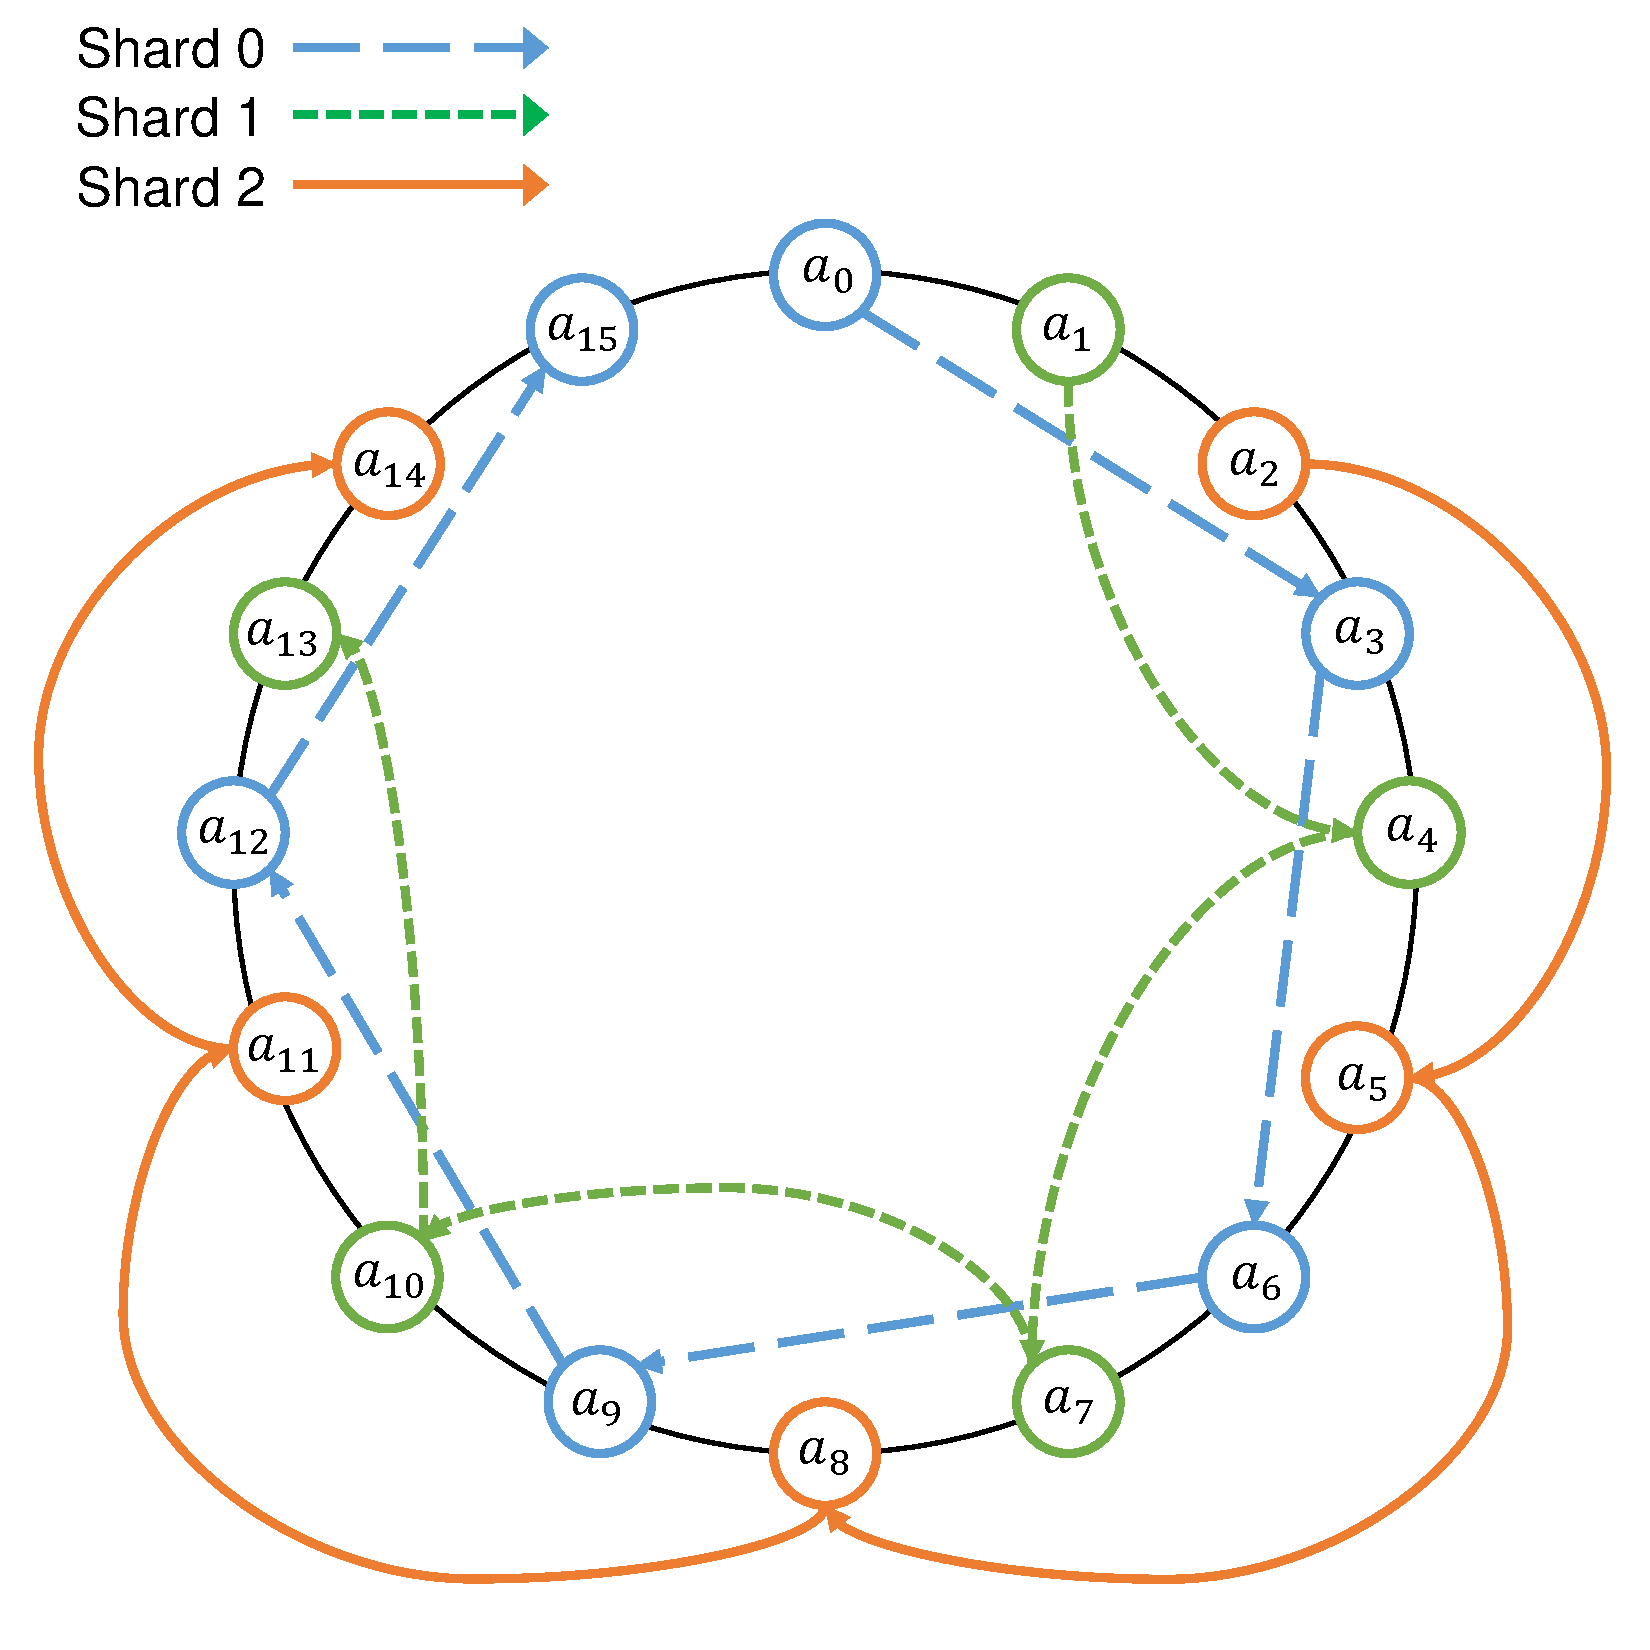
\includegraphics[width=\linewidth]{\ZippyFigures/shard_diagram.pdf}
\caption{\textbf{Sharding Visualization}\,---\,%
This is a configuration with three shards ($n = 3$). Shards $0,1,2$ are
initialized with starting addresses $a_0,a_1,a_2$. Each arrow represents
performing $a_i \cdot g^3$, a step forward by three elements in the
permutation.
}
\label{fig:sharding}
\end{figure}

\paragraph{Benchmarks}
To measure the impact of sharding in isolation from our other enhancements,
we conducted a series of scans, each covering a 1\% sample of the IP address
space, using our local blacklist file and a 10\,GigE uplink. Without
sharding, the average bandwidth utilization over 10~scans was 1.07 Gbps; with
sharding, the average increased to 1.80 Gbps, an improvement of 68\%.

\subsection{Blacklisting and Whitelisting}
 
ZMap address constraints are used to limit scans to specific areas of the
network (whitelisting) or to exclude particular address ranges
(blacklisting), such as IANA reserved allocations~\cite{iana}. Blacklisting
can also be used to comply with requests from network operators who want to
be excluded from receiving probe traffic. Good Internet citizenship demands
that ZMap users honor such requests, but after many scans over a prolonged
time period, a user's blacklist might contain hundreds of excluded prefixes.
 
Even with complicated address constraints, ZMap must be able to efficiently
determine whether any given IP address should be part of the scan. To support
10\,GigE linespeed, we implemented a combination tree- and array-based data
structure that can efficiently manipulate and query allowed addresses.

The IPv4 address space is modeled as a binary tree, where each node
corresponds to a network prefix. For example, the root represents 0.0.0.0/0,
and its children, if present, represent 0.0.0.0/1 and 128.0.0.0/1. Each
\emph{leaf} is colored either white or black, depending on whether or not the
corresponding prefix is allowed to be scanned. ZMap constructs the tree by
sequentially processing whitelist and blacklist entries that specify CIDR
prefixes. For each prefix, ZMap sets the color of the corresponding leaf,
adding new nodes or pruning the tree as necessary.

Querying whether an address may be scanned involves walking the tree,
beginning with the most significant bit of the address, until arriving at a
leaf and returning the color. However, a slightly different operation is used
during scanning. To make efficient use of the pseudorandom permutation
described above, we determine the number of allowed addresses $n$ (which may
be much smaller than the address space if a small whitelist is specified) and
select a permutation of approximately the same size. We then map from this
permutation of $1,\ldots,n$ to allowed addresses $a_1,\ldots,a_n$. Each node
in the tree maintains the total number of allowed addresses covered by its
descendants, allowing us to efficiently find the $i$th allowed address using
a simple recursive procedure.
%The ability to find specific addresses allows ZMap to utilize smaller cyclic
%groups to iterate over a small number of disjoint regions of address instead
%of iterating over the entire address space.\looseness=-1
 
As a further optimization, after the tree is constructed, we assemble a list
of /20 prefixes that are entirely allowed and reassign the address indices so
that these prefixes are ordered before any other allowed addresses. We then
use an array of these prefixes to optimize address lookups. If there are $m$
/20 prefixes that are allowed, then the first $m\cdot2^{12}$ allowed
addresses can be returned using only an array lookup, without needing to
consult the tree. The /20 size was determined empirically as a trade off
between lookup speed and memory usage.
 
\subsection{Zero-Copy NIC Access}
\label{sec:zc}
 
Despite ZMap's use of raw Ethernet sockets, sending each probe packet is an
expensive operation, as it involves a context switch for the \texttt{sendto}
system call and requires the scan packet to be transferred through kernel
space to the NIC~\cite{pfring-original, ten-gig-commodity}. Even with our
other enhancements, the high cost of these in-kernel operations prevented
ZMap from reaching above 2\,Gbps. To reduce these costs, we reimplemented
ZMap's network functionality using the PF\_RING ZC
interface~\cite{pfring-zc}. PF\_RING ZC allows userspace code to bypass the
kernel and have direct ``zero-copy'' access to the NIC\@, making it possible
to send packets without any context switches or wasted memory bandwidth.
 
To boost ZMap to 10\,GigE speeds, we implemented a new probe transmission
architecture on top of PF\_RING\@. This new architecture uses multiple
\emph{packet creation} threads that feed into a single \emph{send} thread. We
found that using more than one send thread for PF\_RING decreased the
performance of ZMap, but that a single packet creation thread was not fast
enough to reach line speed. By decoupling packet creation from sending, we
are able to combine the parallelization benefits of sharding with the speed
of PF\_RING\@.

In the original version of ZMap, multiple send threads each generated and
sent packets via a thread-specific raw Ethernet socket. We modify thread
responsibilities such that each packet creation thread iterates over one
address generation shard and generates and queues the packets. In a tight
loop, each packet generation loop calculates the next index in the shard,
finds the corresponding allowed IP address using the address constraint tree,
and creates an addressed packet in the PF\_RING ZC driver's memory. The
packet is added to a per-thread single-producer, single-consumer packet
queue. The send thread reads from each packet queue as packets come
available, and sends them over the wire using PF\_RING\@.

To determine the optimal number of packet creation threads, we performed a
series of tests, scanning for 50 seconds using 1--6 packet creation threads,
and measured the send rate. We find the optimal number of threads corresponds
with assigning one per physical core.
% Our results are show in Figure~\ref{fig:threads}.

\if0
\begin{figure}\centering
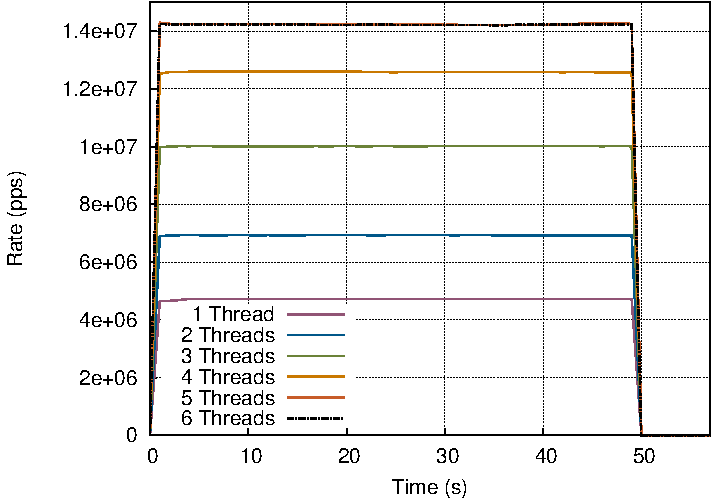
\includegraphics[width=\linewidth]{threads_vs_send.pdf}
\caption{\textbf{Threads vs.\ Scan Rate}\,---\,%
The send rate scales with the number of threads until reaching five threads,
at which point one thread is assigned per physical CPU. As threads begin to
share the same CPU, the send rate peaks. Using six threads results in an
identical send rate to five threads.
}
\label{fig:threads}
\end{figure}
\fi

\if0
\paragraph{Benchmarks}
We compared zero-copy NIC access to ZMap's traditional packet sending
architecture. In each case we also enabled the enhancements discussed in
Section~\ref{sec:TK} and Section~\ref{sec:TK} and conducted repeated scans of
covering 2\% samples of the public IPv4 address space. The average
transmission rate improved from 2.6~Mpps to 14.23~Mpps, a 447\% improvement.
This is 96\% of the theoretical limit of 10\,GigE,
14.88~Mpps~\cite{ten-gig-commodity}.
\fi

\begin{table}\centering
    \begin{tabular}{lrr}
    \toprule
    \textbf{Scan Rate} & \textbf{Hit Rate} & \textbf{Duration} \\ \midrule
    1.44 Mpps ($\approx$1\,GigE)                 & 1.00  & 42:08               \\ 
    3.00 Mpps                  & 0.99  & 20:47              \\ 
    4.00 Mpps                  & 0.97  & 15:38              \\
    14.23 Mpps ($\approx$10\,GigE)                 &  0.63 &  4:29               \\ % raw is 0.675
    \bottomrule
    \end{tabular}
    % 0.675
\caption{\textbf{Performance of Internet-wide Scans}\,---\,%
We show the scan rate, the normalized hit rate, and the scan duration (m:s)
for complete Internet-wide scans performed with optimized ZMap.}
\label{tbl:fullhitrate}
\end{table}

\section{Evaluation}
\label{sec:evaluation}

We performed a series of experiments to characterize the behavior of scanning
at speeds greater than 1~Gbps. In our test setup, we completed a full scan of
the public IPv4 address space in 4m29s on a server with a 10\,GigE uplink.
However, at full speed the number of scan results (the hit rate) decreased by
37\% compared to a scan at 1~Gbps, due to random packet drop. We find that we
can scan at speeds of up to 2.7~Gbps before seeing a substantial drop in hit
rate.

We performed the following measurements on a Dell PowerEdge R720 with two
Intel Xeon E5-2690 2.9~GHz processors (8 physical cores each plus
hyper-threading) and 128~GB of memory running Ubuntu 12.04.4~LTS and the
3.2.0-59-generic Linux kernel. We use a single port on a Intel X540-AT2
(rev~01) 10\,GigE controller as our scan interface, using the PF\_RING-aware
\texttt{ixgbe} driver bundled with PF\_RING 6.0.1. We configured ZMap to use
one send thread, one receive thread, one monitor thread, and five packet
creation threads.

We used a 10\,GigE network connection at the University of Michigan Computer
Science and Engineering division connected directly to the building uplink,
an aggregated $2\times 10$\,GigE channel. Beyond the 10\,GigE connection, the
only special network configuration arranged was static IP addresses. We note
that ZMap's performance may be different on other networks depending on local
congestion and upstream network conditions.\looseness=1

We performed all of our experiments using our local blacklist file. Our
blacklist, which eliminates non-routable address space and networks that have
requested exclusion from scanning~\cite{state-of-scanning}, consists of over
1,000 entries of various-sized network blocks. It results in 3.7~billion
allowed addresses---with almost all the excluded space consisting of IANA
reserved allocations.

\subsection{Hit-rate vs.\ Scan-rate}

In our original ZMap study, we experimented with various scanning speeds up
to gigabit Ethernet line speed (1.44~Mpps) and found no significant effect on
the number of results ZMap found~\cite{zmap}. In other words, from our
network, ZMap did not appear to miss any results when it ran faster up to
gigabit speed.

In order to determine whether hit-rate decreases with speeds higher than
1~Gigabit, we performed 50~second scans at speeds ranging from 0.1--14~Mpps.
We performed 3~trials at each scan rate. As can be seen in
Figure~\ref{fig:hitrate}, hit-rate begins to drop linearly after 4~Mpps. At
14~Mpps (close to 10\,GigE linespeed), the hit rate is 68\% of the hit rate
for a 1\,GigE scan. However, it is not immediately clear why this packet drop
is occurring at these higher speeds---are probe packets dropped by the
network, responses dropped by the network, or packets dropped on the scan
host due to ZMap?

\begin{figure}[t]\centering
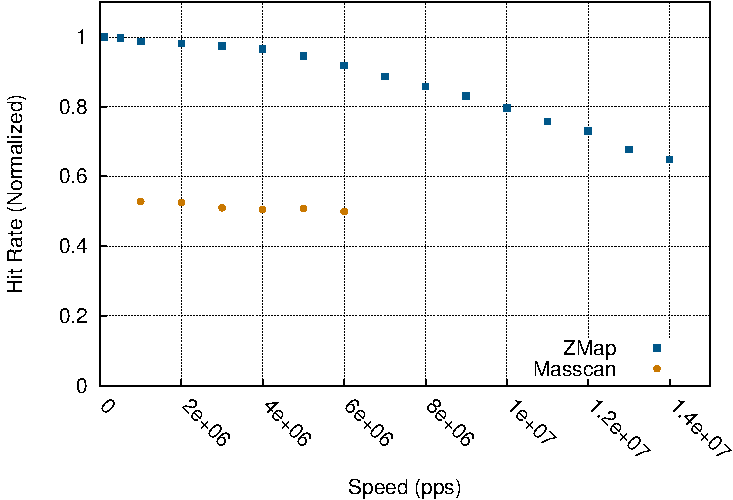
\includegraphics[height=2.1in]{\ZippyFigures/norm_avg_hitrate.pdf}
\caption{\textbf{Hit-rate vs.\ Scan-rate}\,---\,%
ZMap's hit rate is roughly stable up to a scan rate of 4~Mpps, then declines
linearly. This drop off may be due to upstreudegrm network congestion. Even using
PF\_RING, Masscan is unable to achieve scan rates above 6.4~Mpps on the same
hardware and has a much lower hit rate.}
\label{fig:hitrate}
\end{figure}

\begin{figure}[t]\centering
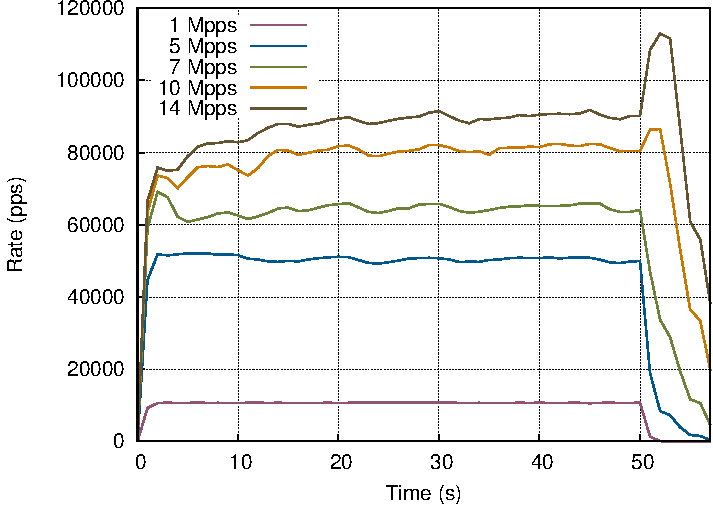
\includegraphics[height=2.1in]{\ZippyFigures/avg_count_recv_succs.pdf}
\caption{\textbf{Response Rate During Scans}\,---\,%
This graph shows the rate of incoming SYN-ACKs during 50-second scans. The
peaks at the end (after sending finishes) at rates above 7~Mpps indicate that
many responses are being dropped and retransmitted before being recorded by
ZMap.}
\label{fig:recvrate}
\end{figure}

We first investigate whether response packets are being dropped by ZMap or
the network. In the original ZMap work, we found that 99\% of hosts respond
within 1~second~\cite{zmap}. As such, we would expect that after 1~second,
there would be negligible responses. However, as can be seen in
Figure~\ref{fig:recvrate}, there is an unexpected spike in response packets
after sending completes at 50~seconds for scans at 10 and 14~Mpps. This spike
likely indicates that response packets are being dropped by our network, NIC,
or ZMap, as destination hosts will resend SYN-ACK packets for more than one
minute if an ACK or RST packet is not received.

In order to determine whether the drop of response packets is due to ZMap
inefficiencies or upstream network congestion, we performed a secondary scan
in which we split the probe generation and address processing onto separate
machines. The send machine remained the same. The receive machine was an HP
ProLiant DL120 G7, with an Intel Xeon E3-1230 processor (4 cores with
hyperthreading) and 16~GB of memory, running Ubuntu 12.04.4~LTS and the
3.5.0-52-generic Linux kernel.

As we show in Figure~\ref{fig:twomachines}, this spike does not occur when
processing response packets on a secondary server---instead it closely
follows the pattern of the slower scans. This indicates that ZMap is locally
dropping response packets. However, the split setup received only 4.3\% more
packets than the single machine---not enough to account for the 31.7\%
difference between a 14~Mpps and a 1~Mpps scan. If a large number of response
packets were dropped due to network congestion, we would not have observed an
immediate drop in responses---likely indicating that the root cause of the
decreased hit-rate is dropped probe packets.

It is not immediately clear where probe packets are dropped---it is possible
that packets are dropped locally by PF\_RING, are dropped by local routers
due to congestion, or that we are overwhelming destination networks. PF\_RING
records locally dropped packets, which remained zero throughout our scans,
which indicates that packets are not being dropped locally. In order to
locate where packet drop is occurring on our network, we calculated the drop
rate per AS and found little AS-level correlation for packets dropped by the
10\,GigE scans, which suggests that random packet drop is occurring close to
our network rather than at particular distant destination networks.

\begin{figure}\centering
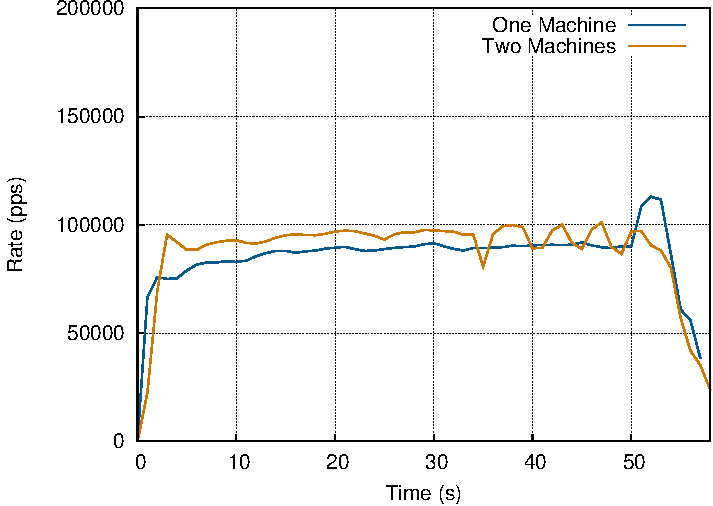
\includegraphics[width=\linewidth]{\ZippyFigures/split_avg_count_recv_succs.pdf}
\caption{\textbf{Comparing One and Two Machines}\,---\,%
If we scan at 14~Mpps and use separate machines for the sending and receiving
tasks, the spike in the SYN-ACK rate at 50~s disappears, indicating that
fewer packets are dropped with the workload spread over two machines.
However, overall the two machine configuration received only 4.3\% more
responses than with one machine, which suggests that network packet loss
accounts for the majority of the drop off at higher scan rates.}
\label{fig:twomachines}
\end{figure}

\subsection{Complete Scans}

We completed a full Internet-wide scan, allowing ZMap to operate at its full
scan rate. This scan achieved an average 14.23~Mpps---96\% of the theoretical
limit of 10\,GigE, completing in 4~minutes, 29~seconds and achieving a hit
rate that is 62.5\% of that from a 1\,GigE scan. We show a comparison to
lower speed scans in Table~\ref{tbl:fullhitrate}. As we discussed in the
previous section, this decrease is likely due to local network congestion,
which results in dropped probe packets. However, more investigation is
deserved in order to understand the full dynamics of high-speed scans.

\subsection{Comparison to Masscan}
\label{sec:masscan-comparison}

\begin{figure*}\centering
\hfill
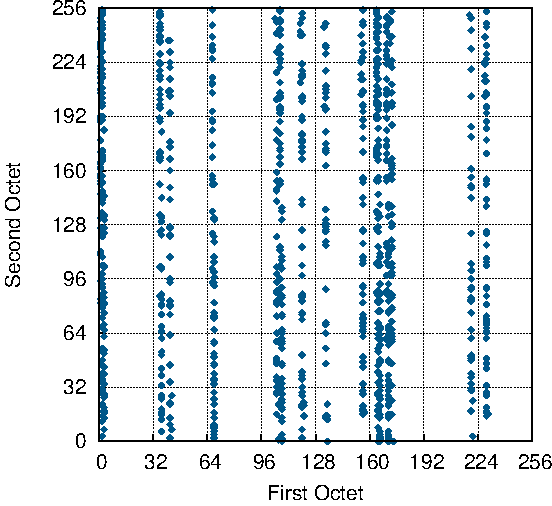
\includegraphics[height=2.5in]{\ZippyFigures/masscan_randomness.pdf}
\hfill\hfill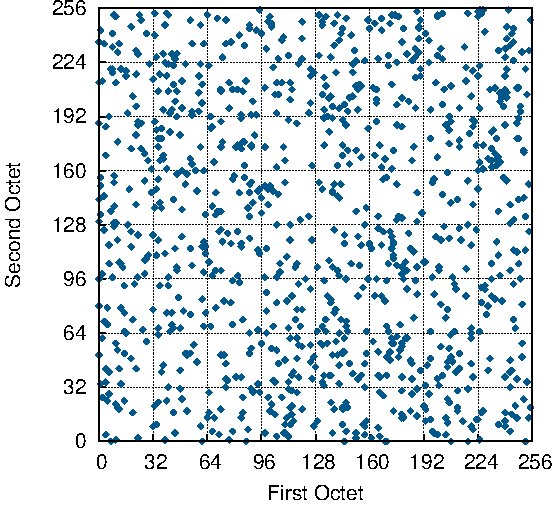
\includegraphics[height=2.5in]{\ZippyFigures/zmap_randomness.pdf}
\hfill\strut
\caption{\textbf{Address Randomization Comparison}\,---\,%
These plots depict the first 1000 addresses of an Internet-wide scan selected
by Masscan (\emph{left}) and ZMap (\emph{right}), with the first and second
octets mapped to the $x$ and~$y$ coordinates. ZMap's address randomization is
CPU intensive but achieves better statistical properties than the cheaper
approach used by Masscan, enabling valid sampling. We enhanced ZMap to
distribute address generation across multiple cores.}
\label{fig:randomy}
\end{figure*}

Masscan advertises the ability to emit probes at 25~Mpps using PF\_RING and
two 10\,GigE adapters, each configured with two RSS queues---84\% of
linespeed for dual 10\,GigE and 166\% of linespeed for a single 10\,GigE
adapter~\cite{masscan-10g}. We benchmarked ZMap and Masscan using the
Xeon~E3-1230 machine described above. In our experiments, we found that
Masscan was able to send at a peak 7.4~Mpps using a single-adapter
configuration with two RSS queues, 50\% of 10\,GigE linespeed. On the same
hardware, ZMap is capable of reaching a peak 14.1~Mpps. While Masscan may be
able to achieve a higher maximum speed using multiple adapters, ZMap is able
to fully saturate a 10\,GigE uplink with a single adapter.

Masscan uses a custom Feistel network to ``encrypt'' a monotonically
increasing index to generate a random permutation of the IPv4 address
space~\cite{masscan-rng}. While this is computation cheaper than using a
cyclic group, this technique results in poor statistical properties, which we
show in Figure~\ref{fig:randomy}. This has two consequences: first, it is not
suitable for sampling portions of the address space, and second, there is
greater potential for overloading destination networks. This could explain
the discrepency in Figure~\ref{fig:hitrate} if Masscan targeted a less
populated subnet.

Masscan and ZMap use a similar sharding approach to parallelize address
generation and distribute scans. Both programs ``count off'' addresses into
shards by staggering the offsets of the starting position of each shard
within the permutation and iterating a fixed number of steps through each of
their permutations. In ZMap, this is implemented by replacing the iteration
factor $g$ with $g^n$. In Masscan, this is simply a matter of incrementing
the monotonically increasing index by more than one.


\section{Applications}
\label{sec:discussion}

In this section, we consider applications that could benefit from 10\,GigE
scanning and remark on the implications of high-speed scanning for defenders
and attackers.

Scanning at faster rates reduces the blur introduced from hosts changing IP
addresses by decreasing the number of hosts that may be doubly counted during
longer scans. This also increases the ability to discover hosts that are only
online briefly. Thus, the ability to complete scans in minutes allows
researchers to more accurately create a snapshot of the Internet at a given
moment.

Similarly, the increased scan rate enables researchers to complete
high-resolution scans when measuring temporal effects. For example, while
researchers were able to complete comprehensive scans for the recent
Heartbleed Vulnerability every few hours~\cite{zmap-heartbleed}, many sites
were patched within the first minutes after disclosure. The ability to scan
more rapidly could help shed light on patching behavior within this critical
initial period.

\begin{figure*}
\centering
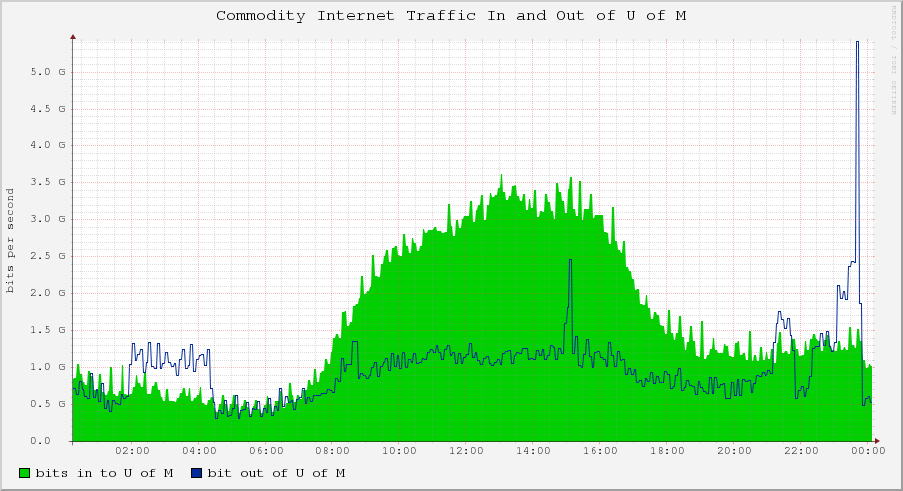
\includegraphics[width=0.75\linewidth]{\ZippyFigures/graph_image.png}
\caption{\textbf{10\,GigE   Scan Traffic}\,---\,%
An Internet-wide scan at full 10\,GigE speed dwarfed all other traffic at the
university during this 24~hour period. At 14.23~Mpps, a single machine
running ZMap generated 4.6~Gbps in outgoing IP traffic and scanned the entire
public IPv4 address space in 4m29s. The massive increase in outbound traffic
appears to have caused elevated packet drop. Notable smaller spikes are due
to earlier experiments.}
\label{fig:traffic}
\end{figure*}

Faster scan rates also allow for a variety of new scanning-related
applications that require multiple packets, including quickly completing
global trace routes or performing operating system fingerprinting.
Furthermore, the advancement of single-port scanning can be utilized to
quickly perform scans of a large number of ports, allowing scanning all
privileged ports on a /16 in under 5~seconds and \emph{all} ports in
5~minutes, assuming the attacker has sufficient bandwidth to the target.

The most alarming malicious potential for 10\,GigE scanning lies in its
ability to find and exploit vulnerabilities \emph{en masse} in a very short
time. Durumeric et~al.\ found that attackers began scanning for the
Heartbleed vulnerability within 22~hours of its
disclosure~\cite{zmap-heartbleed}. While attackers have utilized botnets and
worms in order to complete distributed scans for vulnerabilities, recent
work~\cite{state-of-scanning} has shown that attackers are now also using
ZMap, Masscan, and other scanning technology from bullet-proof hosting
providers in order to find vulnerable hosts. The increase in scan rates could
allow attackers to complete Internet-wide vulnerability scans in minutes as
10\,GigE becomes widely available.\looseness=-1

\section{Future Work}

We demonstrated that it is possible to perform Internet-wide scans at
10\,GigE linespeed, but, at least from our institutional network, we are
unable to sustain the expected hit rate as scanning approaches this packet
rate. Further investigation is needed to understand this effect and profile
ZMap's performance on other networks. One important question is whether the
drop off is caused by nearby network bottlenecks (which might be reduced with
upgraded network hardware) or whether it arises because such rapid scanning
induces congestion on many distant networks---which would represent an
inherent limit on scan speed. It is also possible that there are a small
number of remote bottlenecks that cause the observed drop in hit rate at high
speeds. In that case, identifying, profiling, and removing these bottlenecks
could improve performance.

40\,GigE hardware currently exists, and 100\,GigE is under
development~\cite{hundred-gig}. As these networks become more widely
available, it may be desirable to optimize and scale Internet-wide scanning
to even higher speeds.

\section{Conclusion}

In this work, we introduced enhancements to the ZMap Internet scanner that
enable it to scan at up to 14.2~Mpps. The three modifications we
present---sharding, optimized address constraints, and integration with
PF\_RING ZC---enable scanning at close to 10\,GigE linespeed. These
modifications are available now on experimental ZMap branches and will be
merged into mainline ZMap.

With these enhancements, we are able to complete a scan of the public IPv4
address space in 4m29s. However, despite having a well provisioned upstream
network, coverage in our experiments drops precipitously when scanning faster
than 4~Mpps. While further research is needed to better characterize and
reduce the causes of this drop off, it may be related to specific conditions
on our network.

As faster network infrastructure becomes more widely available, 10\,GigE
scanning will enable powerful new applications for both researchers and
attackers.

\section*{Acknowledgments}

The authors thank the exceptional sysadmins at the University of Michigan for
their help and support throughout this project. This research would not have
been possible without Kevin Cheek, Chris Brenner, Laura Fink, Paul Howell,
Don Winsor, and others from ITS, CAEN, and DCO\@. We are grateful to Michael
Bailey for numerous productive discussions, to Luca Deri and ntop for
providing a PF\_RING license, and to the many contributors to the ZMap open
source project. We also thank Denis Bueno, Jakub Czyz, Henry Fanson, Pat
Pannuto, and Eric Wustrow.

This material is based upon work supported by the National Science Foundation
under Grant No.~CNS-1255153 and No.~CNS-0964545. Any opinions, findings, and
conclusions or recommendations expressed in this material are those of the
authors and do not necessarily reflect the views of the National Science
Foundation.

%% !TEX root = ../../../proposal.tex

{\footnotesize\bibliographystyle{abbrv}
\balance
\bibliography{woot}}
\end{document}



\chapter{Measuring Diffie-Hellman}
\label{chapter:subgroup}
% !TEX root = ../../../proposal.tex

\newcommand{\SubgroupPaper}{papers/subgroup/paper}
\newcommand{\SubgroupFigures}{papers/subgroup/figures}

%\begin{abstract}
%Several recent standards, including NIST~SP~800-56A and RFC~5114, advocate the
%use of ``DSA'' parameters for Diffie-Hellman key exchange.  While it is
%possible to use such parameters securely, additional validation checks are
%necessary to prevent well-known and potentially devastating attacks.  In this
%paper, we observe that many Diffie-Hellman implementations do not properly
%validate key exchange inputs. Combined with other protocol properties and
%implementation choices, this can radically decrease security.
%We measure the prevalence of these parameter choices in the wild
%for HTTPS, POP3S, SMTP with STARTTLS, SSH, IKEv1, and IKEv2, finding millions
%of hosts using DSA and other non-``safe'' primes for Diffie-Hellman key
%exchange, many of them in combination with potentially vulnerable behaviors.
%We examine over 20 open-source cryptographic libraries and applications and
%observe that until January 2016, not a single one validated subgroup orders by
%default.  We found feasible full or partial key recovery vulnerabilities in
%OpenSSL, the Exim mail server, the Unbound DNS client, and Amazon's load
%balancer, as well as susceptibility to weaker attacks in many other applications.
%\end{abstract}

\newcommand{\ScanTable}{
\begin{table*}[]
    \centering\small
    \begin{tabularx}{\textwidth}{Xrrrrrr}
          \toprule
          \hfill & \hfill & \hfill & \multicolumn{4}{c}{{\bfseries\itshape Number of hosts that use\dots}} \\
          \cmidrule{4-7}
          \textbf{Protocol} & \textbf{Scan Date} & \textbf{Total Hosts} & \textbf{Diffie-Hellman} & \twolinecell{\textbf{Non-Safe}\\ \textbf{Primes}} & \twolinecell{\textbf{Static}\\ \textbf{Exponents}} & \twolinecell{\textbf{Static Exponents and}\\\textbf{Non-Safe Primes}} \\
          \midrule
          HTTPS         & 2/2016  & 40,578,754 & 10,827,565 & 1,661,856   & 964,356 & 309,891 \\
          POP3S         & 10/2015  & 4,368,656  & 3,371,616  & 26,285      & 32,215  & 25      \\
          STARTTLS	& 10/2015  & 3,426,360  & 3,036,408  & 1,186,322   & 30,017  & 932     \\
          SSH           & 10/2015  & 15,226,362 & 10,730,527 & 281         & 1,147   & 0       \\
          IKEv1         & 2/2016  & 2,571,900  & 2,571,900  & 340,300     & 109     & 0       \\
          IKEv2         & 2/2016  & 1,265,800  & 1,265,800  & 177,000     & 52      & 0       \\
          \bottomrule
    \end{tabularx}
    \caption{\textbf{IPv4 non-safe prime and static exponent usage}\,---\,%
    Although non-safe primes see widespread use across most protocols, only a
    small number of hosts reuse exponents and use non-safe primes; these hosts
    are prime candidates for a small subgroup key recovery attack.
    }
    \label{tab:scandata}
\end{table*}
}

\newcommand{\HTTPSPrimeTable}{
\begin{table}[]
    \centering\small
    \begin{tabularx}{l|l}
          \toprule
          Prime & Host Count \\
          \midrule
          RFC 5114 Group 22& 1,938,215 \\
          Amazon Load Balancer & 344,148 \\
          Java 768/160 group &  168,949 \\
          Java 1024/160 group & 59,952 \\
          RFC 5114 Group 24 & 3,684 \\
          Java 2048/224 group & 1,142\\
          Epson Devices & 639 \\
          RFC 5114 Group 23 & 437 \\
          \midrule
          Total Using Non-safe Primes & 2,523,493\\
          \bottomrule
    \end{tabularx}
    \caption{\textbf{Top HTTPS non-safe primes}}
    \label{tab:scandata1}
\end{table}
}

\newcommand{\SMTPPrimeTable}{
\begin{table}[]
    \centering\small
    \begin{tabular}{l|l}
          \toprule
          Prime & Host Count \\
          \midrule
          RFC5114 2048/224 group & 1,140,363\\
          Java 1024/160 group & 2,445\\
          Mistyped OpenSSL 512 group & 717 \\
          Java 768/160 group & 671 \\
          \midrule
          Total Using Non-safe Primes & 1,186,322\\
          \bottomrule
    \end{tabular}
    \caption{\textbf{Top SMTP non-safe primes}}
    \label{tab:scandata2}
\end{table}
}

\newcommand{\POPPrimeTable}{
\begin{table}[t]
    \centering\small
    \begin{tabular}{l|l}
          \toprule
          Prime & Host Count \\
          \midrule
          Java 768/160 group & 16,515 \\
          Java 1024/160 group & 9,510 \\
          RFC5114 1024/160 group  & 86 \\
          Java 2048/224 group & 20\\
          \midrule
          Total Using Non-safe Primes & 26,285\\
          \bottomrule
    \end{tabular}
    \caption{\textbf{Top POP3S Non-safe primes}}
    \label{tab:scandata3}
\end{table}
}

\newcommand{\IKEGroupSupportTable}{
\begin{table}[t]
    \centering\small
    \begin{tabularx}{\columnwidth}{Xrr}
          \toprule
          \textbf{Group} & \textbf{IKEv1} & \textbf{IKEv2} \\
          \midrule
          Group 22 & 320.7\,K    & 170.1\,K   \\
          Group 23 & 323.5\,K    & 169.7\,K   \\
          Group 24 & 340.3\,K    & 177\,K   \\
          \midrule
          Baseline & 1907.1\,K  & 1265.8\,K \\
          \bottomrule
    \end{tabularx}
    \caption{\textbf{IKE support for RFC5114 groups}\,---\,%
    We measured support for RFC5114 DSA groups in IKEv1 and IKEv2 by performing
    100\% IPv4 scans and counting how many hosts reply with a valid key exchange
    message for the selected group.}
    \label{tab:ikegroupsupport}
\end{table}
}

\newcommand{\IKEHostValidationTable}{
\begin{table}[t]
    \centering\small
    \begin{tabularx}{\columnwidth}{Xrr}
          \toprule
          \textbf{KE Value}      & \textbf{IKEv1} & \textbf{IKEv2} \\
          \midrule
          $1 \bmod p$   & 89.1\,K  & 1        \\
          $-1 \bmod p$  & 88.7\,K  & 0        \\
          $g_3 \bmod p$ & 318.8\,K & 164.9\,K   \\
          \midrule
          Group 23 Support         & 323.5\,K & 169.7\,K   \\
          \bottomrule
    \end{tabularx}
    \caption{\textbf{IKE validation}\,---,%
    In a 100\% IPv4 scan in February 2016, we measured the number of IKE hosts that accepted various key exchange
    values from Group 23. $g_3$ is a generator of a subgroup with order 3.}
    \label{tab:ikevalidation}
\end{table}
}

\newcommand{\IKEGroupSupportAndValidationTable}{
  \begin{table*}[]
    \centering\small
    \begin{tabularx}{\textwidth}{rXrrrr}
      \toprule

      \hfill & \hfill & \hfill & \multicolumn{3}{c}{{\bfseries\itshape Client key exchange public values offered\dots}} \\
      \cmidrule{4-6}
      \textbf{Protocol} & \textbf{Groups Offered} & \textbf{Support} & \boldmath{$1 \bmod p$} & \boldmath{$-1 \bmod p$} & \boldmath{$g_s \bmod p$} \\
      \midrule
      % Note: Changing the numbers in the support column to be max{support, 1, -1, g_s}
      \textbf{IKEv1} & Group 22 & 332.4\,K & 82.6\,K & 78.5\,K & 332.4\,K \\
      & Group 23 & 333.4\,K & 82.5\,K & 82.5\,K & 333.4\,K \\
      & Group 24 & 379.8\,K & 93.9\,K & 95.2\,K & 379.8\,K \\
      & Baseline (Groups 2, 14, 22, 23, 24) & 1139.3\,K & -- & -- & -- \\
      \midrule
      \textbf{IKEv2} & Group 22 & 182.1\,K & 553 & 553 & 181.9\,K \\
      & Group 23 & 181.9\,K & 542 & 550 & 180.1\,K \\
      & Group 24 & 213.0\,K & 2245 & 2173 & 200.0\,K \\
      & Baseline (Groups 2, 14, 19, 20, 22, 23, 24) & 1203.7\,K & -- & -- & -- \\
      \bottomrule
    \end{tabularx}
    \caption{\textbf{IKE group support and validation}\,---\,%
    We measured support for RFC5114 DSA groups in IKEv1 and IKEv2 and test for key exchange validation by performing a series of 100\% IPv4 scans in October 2016. For Group 23, $g_s$ is a generator of a subgroup with order 3, and for Groups 22 and 24, $g_s$ is a generator of a subgroup of order 7. }
    \label{tab:ikegroupsupportandvalidation}
  \end{table*}
}

\newcommand{\TLSHostValidationTable}{
\begin{table}[b]
    \centering\small
    \begin{tabularx}{\columnwidth}{Xrr}
          \toprule
          \textbf{Key Exchange Value} & \textbf{Support DHE} & \textbf{Accepted} \\
          \midrule
          %$ \texttt{baseline} \bmod p$ & 142.2\,K & 139.2\,K \\
          $0 \bmod p$       & 143.5\,K & 87 \\
          $1 \bmod p$       & 142.2\,K & 4.9\,K \\
          $-1 \bmod p$      & 143.5\,K & 7.6\,K \\
          $g_7 \bmod p$     & 10.7\,K  & 1.5\,K \\
          \bottomrule
    \end{tabularx}
    \caption{\textbf{TLS key exchange validation}\,---\,%
    We performed a 1\% HTTPS scan in August 2016 to check if servers validated received client key exchange values, offering generators of subgroups of order $1$, $2$ and $7$.  Our baseline DHE support number counts hosts willing to
    negotiate a DHE key exchange, and in the case of $g_7$, if $p-1$ is
    divisible by $7$. We count hosts as ``Accepted'' if they reply to the
    \texttt{ClientKeyExchange} message with a \texttt{Finished} message.  For $g_7$, we expect this to happen with probability $1/7$, suggesting that nearly all of the hosts in our scan did not validate subgroup order.}
    \label{tab:tlsvalidation}
\end{table}
}

\newcommand{\SSHHostValidationTable}{
\begin{table}[b]
    \centering\small
    \begin{tabularx}{\columnwidth}{Xrr}
          \toprule
          \textbf{Key Exchange Value} & \textbf{Handshake Initiated} & \textbf{Accepted} \\
          \midrule
          $0 \bmod p$       & 175.6\,K & 5.7\,K \\
          $1 \bmod p$       & 175.0\,K & 43.9\,K \\
          $-1 \bmod p$      & 176.0\,K & 59.0\,K \\
          \bottomrule
    \end{tabularx}
    \caption{\textbf{SSH validation}\,---\,%
    In a 1\% SSH scan performed in February 2016, we sent the key exchange
    values $y_c = 0, 1$ and $p-1$. We count hosts as having initiated a handshake if they send a
    \texttt{SSH\_MSG\_KEX\_DH\_GEX\_GROUP}, and we count hosts as ``Accepted'' if
    they reply to the client key exchange message with a \texttt{SSH\_MSG\_KEX\_DH\_GEX\_REPLY}.}
    \label{tab:sshvalidation}
\end{table}
}

\newcommand{\TLSGroupSupport}{
\begin{table}[b]
    \centering\small
    \begin{tabularx}{\columnwidth}{Xlr}
          \toprule
          \textbf{Company} & \textbf{Product(s)} & \textbf{Count} \\
          \midrule
          Ubiquiti Networks         & airOS/EdgeOS      & 272,690 \\
          Cisco                     & DPC3848VM Gateway & 65,026  \\
          WatchGuard                & Fireware XTM      & 62,682  \\
          Supermicro                & IPMI              & 42,973  \\
          ASUS                      & AiCloud           & 39,749  \\
          Electric Sheep Fencing    & pfSense           & 14,218  \\
          Bouygues Telecom          & Bbox              & 13,387  \\
          Other                     & ---               & 135,432 \\
          \bottomrule
    \end{tabularx}
    \caption{\textbf{HTTPS support for RFC5114 Group 22}\,---\,%
    In a 100\% HTTPS scan performed in October 2016, we found that of the
    12,835,911 hosts that accepted Diffie-Hellman key exchange, 901,656
    used Group~22. We were able to download default web pages for 646,157 of these hosts, which we examined to
    identify companies and products.}
    \label{tab:tls-group22-support}
\end{table}
}



\newcommand{\ECMDistributionTable}{
\begin{table*}[t]
  \centering\small
    \begin{tabularx}{\textwidth}{Xrrrrrrrrr}
    \toprule
      \textbf{Prime} & \multicolumn{7}{c}{\textbf{Exact Order Known}} & \multicolumn{2}{c}{\textbf{Exact Order Unknown}}\\
      \cmidrule(lr){1-1} \cmidrule(lr){2-8} \cmidrule(lr){9-10}
      $\lg(p)$ & 160 bits   & 224 bits  & 256 bits  & 300 bits   & $\lg(p) - 8$   & $\lg(p) - 32$  & $\lg(p) - 64$  & Unlikely DSA & Likely DSA \\
      \midrule
      512   & 3  & 0 & 0 & 0 & 5     & 0   & 0   & 760   & 43     \\
      768   & 4  & 0 & 0 & 4 & 2,685 & 0   & 0   & 220   & 1,402  \\
      1024  & 29 & 0 & 0 & 0 & 323   & 944 & 176 & 1,559 & 26,881 \\
      2048  & 0  & 1 & 1 & 0 & 0     & 0   & 0   & 1,128 & 4,890   \\
      3072  & 0  & 0 & 0 & 0 & 0     & 5   & 0   & 9     & 152    \\
      4096  & 4  & 0 & 0 & 0 & 0     & 0   & 0   & 20    & 183    \\
      8192  & 0  & 0 & 0 & 0 & 0     & 0   & 0   & 0     & 1      \\
      Other & 0  & 0 & 0 & 0 & 0     & 0   & 0   & 400   & 15     \\

      \bottomrule
    \end{tabularx}
    \caption{\textbf{Distribution of orders for groups with non-safe primes}\,---\,%
    For groups for which we were able to determine the subgroup order exactly,
    160-bits subgroup orders are common. We classify other groups to
    be likely DSA groups if we know that the subgroup order is at least 8 bits
    smaller than the prime.
    }
  \label{tab:ecm-distribution}
\end{table*}
}

\newcommand{\ECMBreakableGroups}{
\begin{table*}[t]
    \centering\small
    \begin{tabularx}{\textwidth}{lrrRRRRRR}
      \toprule
      & \multicolumn{2}{c}{{\bfseries\itshape Work (bits)}} & \multicolumn{2}{c}{{\bfseries\itshape HTTPS}} & \multicolumn{2}{c}{{\bfseries\itshape MAIL}} & \multicolumn{2}{c}{{\bfseries\itshape SSH}} \\
       \cmidrule(lr){2-3} \cmidrule(lr){4-5} \cmidrule(lr){6-7} \cmidrule(lr){8-9}
      \textbf{Exponent} & \textbf{Online}    & \textbf{Offline}   & \textbf{Groups}    & \textbf{Hosts} & \textbf{Groups}    & \textbf{Hosts}     & \textbf{Groups}    & \textbf{Hosts}  \\
      \midrule
      160       & 20        & 30        & 3         & 2     & 3         & 7         & 0         & 0      \\
      160       & 30        & 45        & 517       & 1,996 & 1963      & 1,143,524 & 11        & 10     \\
      160       & 40        & 60        & 3,701     & 8,495 & 13,547    & 1,159,853 & 109       & 68     \\
      224       & 20        & 30        & 0         & 0     & 0         & 0         & 0         & 0      \\
      224       & 30        & 45        & 2         & 2     & 14        & 16        & 0         & 0      \\
      224       & 40        & 60        & 307       & 691   & 1039      & 1,141,840 & 3         & 1      \\
      256       & 20        & 30        & 0         & 0     & 0         & 0         & 0         & 0      \\
      256       & 30        & 45        & 0         & 0     & 1         & 1         & 0         & 0      \\
      256       & 40        & 60        & 42        & 478   & 180       & 1,140,668 & 0         & 0      \\
      \bottomrule
    \end{tabularx}
    \caption{\textbf{Full key recovery attack complexity}\,---\,%
    We estimate the amount of work required to carry out a small subgroup key
    recovery attack, and show the prevalence of those groups in the wild. Hosts
    are vulnerable if they reuse exponents and fail to check subgroup order.
    }
  \label{tab:ecm-breakable}
\end{table*}
}

\newcommand{\ECMRFCFiveFiveOneFourGroups}{
\begin{table}[b]
    \centering\small
    \begin{tabularx}{\columnwidth}{Xrrr}
          \toprule
          \textbf{Group} & \textbf{Exponent Size} & \textbf{Online Work} & \textbf{Offline Work} \\
          \midrule
          Group 22 & 160 & 8  & 72 \\
          Group 23 & 224 & 33 & 47 \\
          Group 24 & 256 & 32 & 94 \\
          \bottomrule
    \end{tabularx}
    \caption{\textbf{Attacking RFC 5114 groups}\,---\,%
    We show the log of the amount of work in bits required to perform a small
    subgroup key recovery attack against a server that both uses a static
    Diffie-Hellman exponent of the same size as the subgroup order and fails to
    check group order.
    }
    \label{tab:ecm-rfc5114}
\end{table}
}

\newcommand{\PrimesAllTLS}{
\begin{table*}[t]
    \centering\small
    \begin{tabularx}{\textwidth}{Xrrrrrr}
        \toprule
        \multicolumn{3}{c}{{\bfseries\itshape Group}} & \multicolumn{4}{c}{{\bfseries\itshape Host Counts}} \\
        \cmidrule(lr){1-3} \cmidrule(lr){4-7}
        \textbf{Source} & \textbf{Prime Size} & \textbf{Subgroup Size} & \textbf{HTTPS} & \textbf{SMTP} & \textbf{POP3S} & \textbf{SSH} \\
        \midrule
        RFC 5114 Group 22            & 1024 & 160    & 1,173,147 & 145       & 86     & 0   \\
        Amazon Load Balancer       & 1024 & 160    & 277,858   & 0         & 1      & 0   \\
        JDK                        & 768  & 160    & 146,491   & 671       & 16,515 & 0   \\
        JDK                        & 1024 & 160    & 52,726    & 2,445     & 9,510  & 0   \\
        RFC 5114 Group 24            & 2048 & 256    & 3,543     & 5         & 0      & 6   \\
        JDK                        & 2048 & 224    & 982       & 12        & 20     & 0   \\
        Epson Device               & 1024 & $<948$ & 372       & 0         & 0      & 0   \\
        RFC 5114 Group 23            & 2048 & 224    & 371       & 1,140,363 & 2      & 0   \\
        Mistyped OpenSSL 512       & 512  & 497    & 0         & 717       & 0      & 0   \\
        \midrule
        Other Non-Safe Primes      & ---  & ---    & 6,366     & 41,964    & 151    & 275 \\
        Safe Primes & --- & --- & 9,165,709 & 1,850,086 & 3,345,331 & 10,730,246 \\
        \midrule
        Total & \hfill & \hfill & 10,827,565 & 3,036,408 & 3,371,616 & 10,730,527 \\
        \bottomrule
    \end{tabularx}
    \caption{\textbf{IPv4 top non-safe primes}\,---\,%
    Nine non-safe primes account for the majority of hosts using non-safe
    primes.
    }
    \label{tab:primes}
\end{table*}
}

\newcommand{\TLSLibraryTable}{
  \begin{table*}[t]
    \centering\small
    \begin{tabularx}{\textwidth}{Xlllll}
        \toprule
        \textbf{Implementation} & \textbf{RFC 5114 Support} & \textbf{Allows Short Exponents} &
        \textbf{Reuses Exponents} & \textbf{Validates Subgroup} &  \\
        \midrule
        Mozilla NSS   & No & Yes, hardcoded
                      & No                         & $g \leq 2$         &  \\
        OpenJDK       & No & Yes, uses max of p\_size / 2 and 384
                      & No                         & $g \leq 2$         &  \\
        OpenSSL~1.0.2 & Yes & Yes, if $q$ set or if user sets a shorter length
                      & Default until Jan '16      & Yes, as of Jan '16 &  \\
        BouncyCastle  & Yes & No
                      & Application dependent      & $g \leq 2$         &  \\
        Cryptlib      & No & Yes, uses quadratic curve calculation
                      & Application dependent      & $g \leq 2$         &  \\
        libTomCrypt   & No & Yes, hardcoded
                      & Application dependent      & No                 &  \\
        CryptoPP      & No & Yes, uses work factor calculation
                      & Application dependent      & No                 &  \\
        Botan         & Yes & Yes, uses work factor calculation
                      & No                         & No                 &  \\
        GnuTLS        & Application dependent & Yes, restricts to q\_size (max 256)
                      & Application dependent      & $g \leq 2$         &  \\
        \bottomrule
    \end{tabularx}
    \caption{\textbf{TLS Library Behavior}\,---\,%
    We examined popular TLS libraries to determine which weaknesses from
    Section~\ref{subsec:small-subgroup-attack} were present. Reuse of exponents
    often depends on the use of the library; the burden is on the application
    developer to appropriately regenerate exponents. Botan and libTomCrypt both
    hardcode their own custom groups, while GnuTLS allows users to specify
    their own parameters.
    }
    \label{tab:tls-implementations}
\end{table*}
}

\newcommand{\GroupOrderFactorization}{
\begin{table*}[ht]
    \centering\footnotesize
    \begin{tabularx}{\textwidth}{lcl}
        \toprule
                            & \textbf{Factored}     &  \\
         \textbf{Source}    & \textbf{Completely?}  & \textbf{Order Factorization} \\
        \midrule
        RFC 5114 Group 22     & Yes & \tt 2\^{}3 * 7 * df * 183a872bdc5f7a7e88170937189 * 228c5a311384c02e1f287c6b7b2d * 5a85 \\
                              &   & \tt 7d66c65a60728c353e32ece8be1 * f518aa8781a8df278aba4e7d64b7cb9d49462353 * 1a3adf8 \\
                              &   & \tt d6a69682661ca6e590b447e66ebd1bbdeab5e6f3744f06f46cf2a8300622ed50011479f18143d471 \\
                              &   & \tt a53d30113995663a447dcb8e81bc24d988edc41f21 \\
        RFC 5114 Group 23     & No & \tt 3\^{}2 * 5 * 2b * 49 * 9d * 5e9a5 * 93ee1 * 2c3f0539 * 136c58359 * 1a30b7358d * 335 \\
                              &   & \tt a378eb0d * 801c0d34c58d93fe997177101f80535a4738cebcbf389a99b36371eb * 22bbe4b573 \\
                              &   & \tt f6fc6dc24fef3f56e1c216523b3210d27b6c078b32b842aa48d35f230324e48f6dc2a10dd23d28d3 \\
                              &   & \tt 82843a78f264495542be4a95cb05e41f80b013f8b0e3ea26b84cd497b43cc932638530a068ecc44a \\
                              &   & \tt f8ea3cc84139f0667100d426b60b9ab82b8de865b0cbd633f41366622011006632e0832e827febb7 \\
                              &   & \tt 066efe4ab4f1b2e99d96adfaf1721447b167cb49c372efcb82923b3731433cecb7ec3ebbc8d67ef4 \\
                              &   & \tt 41b5d11fb3328851084f74de823b5402f6b038172348a147b1ceac47722e31a72fe68b44ef4b \\
        RFC 5114 Group 24     & Yes & \tt 7 * d * 9f5 * 22acf * bd9f34b1 * 8cf83642a709a097b447997640129da299b1a47d1eb3750 \\
                              &   & \tt ba308b0fe64f5fbd3 * 15adfe949ebb242e5cd0978fac1b43fdbd2e5b0c5f48924fbbd370195c0e \\
                              &   & \tt b20596d98ad0a9e3fd98876413d926f41a8b918d2ec4b018a30efe5e336bf3c7ce60d515cf46af5f \\
                              &   & \tt acf3bb389f68ad0c4ed2f0b1dbb970293741eb6509c64e731802259a639a7f57d4a9c0d9445241f5 \\
                              &   & \tt bcdbdc50555b76d9c335c1fa4e11a8351f1bf4730dd67ffed877cc13e8ea40c7d51441c1f4e59155 \\
                              &   & \tt ef1159eca75a2359f5e0284cd7f3b982c32e5c51dbf51b45f4603ef46bae528739315ca679703c1f \\
                              &   & \tt fcf3b44fe3da5999daadf5606eb828fc57e46561be8c6a866361 \\
        Amazon Load           & No & \tt 2 * 3 * 5 * edb * 181ac5dbfe5ce13b * 18aa349859e9e9de09b7d65 * 9414a18a7b575e8f4 \\
        Balancer              &   & \tt 2f6cb2dbc22eb1fc21d4929 * 2de9f1171a2493d46a31d508b63532cdf86d21db6f50f717736fc4 \\
                              &   & \tt b0b722856a504ed4916e0484fe4ba5f5f4a9fff28a1233b728b3d043aec37c4f138ffd58fe7a8c3c \\
                              &   & \tt 1e93cb52be527395e45db487b61daadded9c8ec35 \\
        Mistyped OpenSSL      & Yes & \tt 5 * b * a9b461e1636f4b51ef * 1851583cf5f9f731364e4aa6cdc2cac4f01* 3f0b39cacfc086 \\
        512 ``Prime'' Factors &   & \tt df4baf46c7fa7d1f4dfe184f9d22848325a91c519f79023a4526d8369e86b \\
        Mistyped OpenSSL      & Yes & \tt 2\^{}13 * 3\^{}3 * 5\^{}2 * 11\^{}2 * 269 * 295 * 4d5 * 97c3 * 9acfe7 * 8cdd0e128f * 385 \\
        512 Order Factors     &   & \tt b564eecd613536818f949 * 146d410923e999f8c291048dc6feffcebf8b9e99eec9a4d585f87422 \\
                              &   & \tt e49b393256c23c9 \\
        \bottomrule
    \end{tabularx}
    \caption{\textbf{Group order factorization for common non-safe primes}\,---\,%
    We used the elliptic curve method to factor $(p-1)/2$ for each of the
    non-safe primes we found while scanning, as well as the mistyped OpenSSL
    ``prime''.
    }
    \label{tab:group-order-factorization}
\end{table*}
}

\newcommand{\ApplicationsTable}{
  \begin{table}[t]
    \centering\small
    \begin{tabularx}{\linewidth}{Xlll}
        \toprule
        \textbf{Application} & \textbf{Crypto}  & \textbf{Short}    & \textbf{Exponent} \\
                             & \textbf{Library} & \textbf{Exponent} & \textbf{Reuse} \\
        \midrule
        OpenSSH     & OpenSSL     & No          & No    \\
        Cerberus    & OpenSSL     & No          & Yes   \\
        GNU lsh     & GnuTLS      & No          & No    \\
        Dropbear    & LibTomCrypt & No          & No    \\
        Lighttpd    & OpenSSL     & Yes         & No    \\
        Unbound     & OpenSSL     & Yes         & Yes   \\
        Exim        & OpenSSL     & Library     & Yes   \\
                    &             & dependent   &       \\
        Postfix     & OpenSSL     & No          & No    \\
        \bottomrule
    \end{tabularx}
    \caption{\textbf{Common application behavior}\,---\,%
    Applications make a diverse set of decisions on how to handle
    Diffie-Hellman exponents, likely due to the plethora of conflicting,
    confusing, and incorrect recommendations available.
    }
    \label{tab:common-applications}
\end{table}
}




% !TEX root = ../proposal.tex

Cryptography is mathematical science. Cryptography research is often formal,
and concerned with proving the correctness of primitives and
protocols, given some set of assumptions. Cryptography is one of the only
components of security that can be provably secure. As such, cryptography is
often considered to be one of the strongest components of security.

Yet historically, cryptography has been one of the most \textit{fragile}
aspects of security. This fragility is often not because the underlying math
was incorrect, or because the fundamental cryptographic primitives were
insecure, but because a single mistake in the implementation, configuration,
or protocol can have catastrophic effects on security. Security is lost in
translation between the cryptographers and protocol designers, and between
protocol designers and implementers. The process of going from paper to
program, or from proof-of-concept to production, introduces mistakes and
misunderstandings and reveals incorrect assumptions. This leads to
cryptographic failures and insecurity.

%To address this, the cryptographic research community is beginning to
%introduce and study new concepts such as misuse-resistant cryptography, and
%simplified cryptographic APIs. Unfortunately, the state of the art in
%cryptography engineering remains considerably behind the state of art in
%research.

Cryptography is a key component in the security of the Internet.
Unfortunately, the fragile nature of cryptography can be compounded by the
large-scale, distributed, and diverse nature of the Internet. Any protocol
can have many implementations, each of which may implement different subsets
of the protocol, or support different configurations. Many protocols are
designed for ``cryptographic agility'', and so identical implementations may
support different sets of underlying algorithms. Devices that support modern
cryptography may also support decades-old broken cryptography. This leads to
an Internet of fragile cryptographic ecosystems, consisting of diverse sets
of clients and servers \todo{define this more}.

%To better use cryptography to secure the Internet, we must first
%understand how cryptography is being used on the Internet. Examining CVE databases
%and trawling through cryptographic code provides one lens into real-world
%deployments of cryptography, but does not necessarily reflect the state of
%the Internet.

To better use cryptography to secure the Internet, we need to understand what
types of cryptography are being used, and where mistakes are being made. We
must understand which cryptographic ecosystems are fragile, and which are
resiliant. Large-scale empirical methods allow us to observe fragility in
how cryptography is being used on the Internet, identify new vulnerabilites,
and better secure the Internet in the future.

In this dissertation, I show how empirical measurements collected using
Internet-wide scanning provides insight into how cryptography is used to
secure the Internet. First, I show contributions made to the field of
Internet measurement field itself via improved Internet-wide scanning.
Second, I measure the Internet's resiliancy to small subgroup attacks in
finite-field Diffie-Hellman. Third, I use empirical methods to show how
1990s-era export-grade encryption harmed the security of the Internet for two
decades.

\section{Techniques for Measuring Internet Cryptography}

Internet-wide scanning is a fundmental technique used for empirical study of
cryptography. Large-scale, horizontal port scanners such as
ZMap~\cite{zmap-2013} drastically reduce the barrier to entry to leveraging
network scan data at Internet scale, however port scanning alone is not a
complete solution. Using Internet-wide scanning to measure cryptography is a
three step process:
\begin{enumerate}
  \item \textbf{Identify Hosts.}
    There are $\sim$4B possible IPv4 addresses, however only a subset are
    listening on any given L4 port. A single scan by ZMap or another
    large-scale, asynchronous L3/L4 scanner identifies which hosts have an
    input port open. For example, only $\sim$50M hosts respond on TCP port 443
    (HTTPS).
  \item \textbf{Measure Hosts.}
    ZMap provides no application-layer information about a host. Furthermore,
    hosts that respond on a standard port for some application-layer protocol
    might not actually be configured to speak that protocol. For example,
    only $\sim$38M of the $\sim$50M hosts with TCP port 443 open are TLS
    servers. To collect cryptographic data, an application-layer scanner such
    as ZGrab~\cite{zgrab-github} must connect to all hosts found by ZMap and
    attempt a protocol handshake that records the cryptographic state used
    for the connection.
  \item \textbf{Answer Questions.}
    As is the case in any empirical science, the measurement data is analyzed
    to answer questions such as ``What percentage of TLS servers support
    512-bit Diffie-Hellman?''. Tools such as Censys~\cite{censys} allow
    researchers to ask questions about Internet-wide scan data much faster
    and easier than by trawling through results from individual scans, each
    of which can generate terabytes of data.
\end{enumerate}

With current technology, Internet-wide scanning is useful for creating an
aggregate understanding of the Internet over time. However, it is not yet
able to provide a global understanding of \textit{individual} hosts and
networks. I first discuss contributions to Internet-wide scanning that
provide a foundation to build a more accurate and complete picture of the
Internet in \S\ref{chapter:zippier}. I show improvements to the ZMap scanner
which enable it to operate at a full 10Gbps line
rate~\cite{zippier-zmap-2014}. While ZMap enabled the use of Internet-wide
scanning accessible as a measurement method, this work moves towards enabling
hourly or real-time measurement of the cryptographic behavior of all
Internet-connected systems.

When originally introduced, ZMap was capable of saturating a 1Gbps uplink from
a single host, enabling an Internet-wide TCP SYN scan of IPv4 to be performed
in forty-five minutes. However, when used with a 10Gbps network interface, ZMap
reached barely above the 1Gbps mark. The required thread synchronization during
address generation restricted the performance benefit of threading, and limited
the ability to leverage multi-core systems. Furthermore, the copy from user
space to kernel memory when sending a packet limited total throughput. Scanning
a 10Gbps requires sending nearly 15 million packets per second continuously,
which allows for only 200 cycles per packet on a 3 GHz system.

I introduced performance improvements to address both of these constraints, and
enable ZMap to fully utilize a 10Gbps network link, bringing the total time for
a TCP SYN scan of IPv4 to under five minutes from a single host. While
Internet-measurement is often used to provide coarse-grain understanding of the
shape of the Internet as a whole, improvements in measurement-collection begin
to move the field towards being able to continuously understand the behavior of
individual hosts, but at global scale.

\section{Measuring Diffie-Hellman}

There is a knowledge gap between implementers and researchers. Cryptographers
can be aware of attacks for decades, but this doesn't necessarily translate
into concrete steps that implementers can take to avoid vulnerability. A
specific example of this is prime-field based Diffie-Hellman key exchange, in
which implementation and hosts often use groups which unnecessarily open up
the likelihood of small-subgroup confinement and key recovery
attacks~\cite{subgroup-2017}. I used empirical techniques to provide insight
into the Diffie-Hellman group selection at Internet-scale, showing that while
a common recommendation is that $p$ should be a ``safe'' prime such that $p =
2q+1$ for some prime $q$, many implementations instead use non-safe ``DSA''
parameters with potentially unsafe subgroups of order $q$. Several standards,
including NIST~SP~800-56A~\cite{sp800} and RFC~5114~\cite{rfc5114}, advocate
the use of these parameters for Diffie-Hellman key exchange, and while it is
possible to use such parameters securely, additional validation checks are
necessary to prevent small-subgroup attacks.

We measured the prevalence of these parameter choices in the wild for HTTPS,
POP3S, SMTP with STARTTLS, SSH, IKEv1, and IKEv2, finding millions of hosts
using DSA and other non-``safe'' primes for Diffie-Hellman key exchange, many
of them in combination with potentially vulnerable behaviors. Beyond simply
using DSA primes, small subgroup attacks require a number of complex, special
conditions to go wrong in order to be feasible, described in
\S\ref{chapter:subgroup}. While seems unlikely that any implementation would
satisfy enough of these requirements to be vulnerable to an attack, it also
seemed unlikely that implementations would use non-safe primes for key
exchange in the first place. Empirical methods did not reveal an
Internet-wide vulnerability, but rather an Internet-wide case of accidental
complexity and fragility. Given the amount of complexity exposed by the
underlying cryptographic APIs for Diffie-Hellman, it is remarkable that any
implementation was safe. Understanding the root causes of this complexity and
confusion, and understanding how it manifests on the Internet, enables better
protocol design in the future.

\section{Measuring Export Cryptography}

%Discrete-log and factoring based attacks are generally considered out of reach
%of attackers.  However, informing such attacks with measurement data allows for
%cost-effective attacks that leverage a single, expensive pre-computation to
%cheaply attack TLS connections. Furthermore, when combined with broad support
%for cryptography that was assumed to be “dead”, these attacks become even
%cheaper.

%\paragraph{Export Cryptography}

The Department of State regulated cryptography in the United States during
the 1990s. Cryptography was covered by the Internation Traffic in Arms
Regulations (ITAR), which broadly limited the ability for US persons to
``export'' cryptography. Beginning in 1995, these regulations were challenged
in court by Daniel J. Bernstein, who was attempting to publish the
``Snuffle'' cryptosystem. The regulations were moved in 1996 from ITAR to the
Export Administration Regulations (EAR), under the control of the Department
of Commerce~\cite{djb-case-status}. Under EAR, ``exported'' cryptography was
limited to 40-bits of security for symmetric ciphers, and 512-bits for
security for public-key cryptography. Authentication strength (\eg MAC
length), was not regulated~\cite{ear-2001-cat-5}. Despite these limitations,
there were major advances in secure channel protocol development during this time.
\ssltwo was designed and deprecated~\cite{sslv2} in 1995. SSLv3 was created and
standardized~\cite{rfc6101} by 1998, and subsequently renamed to TLS and
moved into the purview of the IETF in 1999~\cite{rfc2246}. All three of these
protocol versions contained compliance mechanisms for the export regulations,
where the protocol was capable of negotiating the use of short
``export-grade'' parameters instead of ``modern'' cryptography.

Following further litigation in \textit{Bernstein vs United States}, the key
length limitations from the export regulations were removed in 1999, and
future versions of TLS deprecated the process for using ``export-grade''
cryptography.

\subsection{Attacks on RSA}

\todo{freak}

\todo{freak measurements}

\subsection{Attacks on Diffie-Hellman}

Diffie-Hellman key exchange is one of the most common public-key
cryptographic methods in use in the Internet. In finite field Diffie-Hellman,
Alice and Bob agree on a large prime $p$ and an integer $g$ modulo $p$. Alice
chooses a secret integer $x_a$ and transmits a public value $g^{x_a} \bmod
p$; Bob chooses a secret integer $x_b$ and transmits his public value
$g^{x_b} \bmod p$. Both Alice and Bob can reconstruct a shared secret $g^{x_a
x_b} \bmod p$, but the best known way for a passive eavesdropper to
reconstruct this secret is to compute the discrete log of either Alice or
Bob's public value. Specifically, given $g$, $p$, and $g^x \bmod p$, an
attacker must calculate $x$.

We uncovered several weaknesses in how finite-field Diffie-Hellman key
exchange was deployed, which drastically affected the cost of decrypting
large amounts of TLS traffic. The algorithmic complexity of calculating
discrete log is exponential, but the bulk of this computation is dependent
solely on $p$, not the individual secrets $a$ and $b$ chosen by each party.
If many hosts use the same groups, then the precomputation cost may be
amortized across all the connections across these hosts, rather than
requiring core-centuries per observed key exchange. This raise an obvious
empirical question: do many hosts share the same set of Diffie-Hellman
parameters, and what is the strength of the parameters?

The TLS protocol contains ``export-grade'' Diffie-Hellman ciphers which use
short 512-bit groups. We show that there is a protocol vulnerability in TLS,
named Logjam, which allows an attacker who can calculate 512-bit discrete logs
to downgrade connections to export-grade Diffie-Hellman ciphers, and decrypt
them. If a TLS session were to use 512-bit Diffie-Hellman, it may first appear
that individual connections could be broken in 60,000 core-hours, or 120 hours
in parallel on commodity hardware. While this is certainly insecure, at first
glance it would appear these connections have a small amount forward secrecy,
by virtue of using ephemeral Diffie-Hellman key, e.g. each connection would
require another 120 hours to be decrypted. This slow process would prohibit
active attacks and limit the risk to passive decryption after the fact. This
again falls prey to precomputation: if many hosts were to support the same weak
parameters, then the computation could be amortized, and individual connections
could be broken in real-time, enabling active attacks. In fact, shared sets of
parameters is what enables the downgrade. In this case, empirical measurement
showed that 80\% of vulnerable hosts used the same set of parameters, moving
this attack from the theoretical to the practical. While recently there has
been a trend towards elliptic curve cryptography, prime-field based
Diffie-Hellman remained common in TLS until 2016, when both Firefox and Chrome
removed it from their default cipher suites as a result of our work.

\subsection{Cross-Protocol Attacks}

Reusing TLS keys across multiple protocols, such as HTTPS, SMTP, and IMAP,
leads to an increased attack surface. Empirical methods allow us to understand
the attack surface increase from key reuse. Furthermore, specific
vulnerabilities in the TLS protocol and older implementations can be utilized
in a cross-protocol context to attack users of a web service without explicitly
compromising the private key. This is best shown by the DROWN vulnerability, in
which the mere existence of an \ssltwo host that shared a key with a TLS host
enabled decryption of otherwise secure TLS connections using modern
cryptography.

The DROWN attack further exploited export-grade cryptography with an additional
novel insight: Bleichenbacher oracles need not be present in the target
protocol under attack, so long as the key is shared between the two protocols.
Specifically, DROWN shows how to use protocol vulnerabilities in \ssltwo to
attack TLS 1.2. The \ssltwo protocol includes support export symmetric ciphers
which are seeded via only five bytes of key material encrypted using RSA \PKCS.
The \ssltwo protocol also requires the server to send data to the client that is
derived from the shared secret, without first verifying that the client has
possession of the secret. When combined with the malleability of RSA,
culminates in a Bleichenbacher oracle that can be used to attack TLS 1.2

Beyond DROWN, the TLS protocol has a fundamentally cross-protocol attack
surface. X.509 certificates are not bound to any particular protocol or port.
Furthermore, even if distinct services, such as mail and web servers, use
different keys, so long as they share any name on the certificate, the
transport-layer security of all connections to that name are limited to the
security of the weakest TLS implementation or configuration. Even traditionally
web-based padding oracle attacks, such as POODLE, or the AES-NI padding-oracle
in OpenSSL, non-web servers can be exploited by active attackers targeting web
users. The attacker can rewrite the TCP connection to an alternative port, and
fill-in any pre-handshake protocol dialogue (e.g. by sending an EHLO or
STARTTLS command in SMTP). Ignoring vulnerabilities in TLS itself, an unpatched
piece of software with a known RCE using the same key as a well-configured and
up to date web server places web clients, should the key be stolen via
traditional software exploitation. We can place an upper bound on the increased
attack surface, by measuring key and name reuse across TLS in different
application-layer protocols on different ports.

\subsection{Weaknesses from Export Cryptography}

As shown by Freak, Logjam, and DROWN, the security of TLS and export
cryptography are fundamentally linked. Export cryptography is a unique
constraint with a fundamentally dangerous goal: weaken cryptography, without
weakening cryptography. Internet measurement techniques show us that the export
regulations weakened protocol design to the point where the regulations are
directly harmful to the security of the Internet today. These empirical
techniques show that these attacks are not theoretical, leveraging protocols
that have long-since disappeared, but instead are a dark side of backwards
compatibility, harming real users today. Although the regulations went out of
effect by 1999, the cryptography remains. At their respective times of
disclosure, 36.7\% of IPv4 HTTPS hosts were vulnerable to FREAK, 4.9\% were
vulnerable to Logjam, and 26\% were vulnerable to DROWN. All forms of export
cryptography have been broken: export RSA key exchange was broken by FREAK,
export Diffie-Hellman key exchange was broken by Logjam, and export symmetric
ciphers were broken by DROWN. In all cases, empirical research enabled the full
understanding of the effects and impacts of these issues.

% CONCLUSION THOUGHTS
% 
% ENGINERING?
% 
% Applying empirical measurement techniques accurately requires careful
% application of the scientific method and experiment design. However, the field
% of Internet-measurement has strong engineering underpinnings which are often
% overlooked. ZMap now provides efficient transport-layer scanning, but
% application-layer scanning has not yet reached the same efficiency as ZMap.
% Tooling such as ZGrab helps fill in some of these gaps, but is not yet
% transformative. Similarly, simply studying HTTPS at scale creates unique
% engineering constraints, such as how to batch parse and validate X.509
% certificates.



%\subsection{Bleichenbacher's Attack.}
%One of the most important attacks in the TLS history is the million's message attack, published by Daniel Bleichenbacher at Crypto 1998~\cite{Bleichenbacher}. The attack targets the RSA \PKCS encryption scheme, which is used in the TLS protocol to encrypt a so called \pms. The \pms a 48 byte value sent by the client to the server, encrypted using server's public key. Based on the \pms, both peers can derive \textit{all} keys needed for secure communication.
%
%Essentially, Bleichenbacher's attack is an adaptive chosen-ciphertext attack or, more commonly known, a padding oracle attack. The attack assumes existence of an oracle that responds with "valid" or "invalid" according to the \PKCS validity of the decrypted message. The attacker exploits such an oracle as follows. It starts the attack with an RSA ciphertext (containing an encrypted \pms), which he obtained for example by observing the traffic between the client and the server. The attacker then modifies this ciphertext, sends it to the server, and observes the ciphertext validity. With each valid ciphertext, the attacker learns several plaintext bits. At the end, by sending several thousands of messages the attacker can decrypt the whole \pms, and thereby decrypt a TLS session.

In the following, $a||b$ denotes concatenation of strings $a$ and
$b$. $a{[i]}$ references the $i$-th byte in $a$.
$(N,e)$ denotes an RSA public key, where $N$ has byte-length
$\ell_m$ ($|N|=\ell_m$) and $e$ is the public exponent. The corresponding
secret exponent is $d = 1/e \bmod \phi(N)$.

\subsection{\PKCS encryption padding}
\label{sec:PKCSdescr}

Our attacks rely on the structure of RSA \PKCS padding.  Although RSA PKCS\#1 v2.0
implements OAEP, SSL/TLS still uses \PKCS.
The \PKCS encryption padding scheme~\cite{rfc2313}
randomizes encryptions by prepending a random padding string $PS$
to a message $k$ (here, a symmetric session key) before
RSA encryption:

\begin{enumerate} 
	\item The plaintext message is $k$, $\ell_k = |k|$. The encrypter generates a random byte
	string $PS$, where $|PS| \geq 8$, $|PS|=\ell_m-3-\ell_k$, and $\hex{00} \not \in \{PS{[1]}, \ldots,PS{[|PS|]}\}$. 
	\item The encryption block is $m = 00||02||PS||00||k$. 
	\item The ciphertext is computed as $c = m^e \bmod N$. 
\end{enumerate} 

To decrypt such a ciphertext, the decrypter first computes $m = c^d
\bmod N$.  Then it checks whether the decrypted message $m$ is
correctly formatted as a \PKCS-encoded message. We say that the
ciphertext $c$ and the decrypted message bytes $m{[1]} || m{[2]} || ... ||
m{[\ell_m]}$ are \PKCSconform if:
\begin{equation*} 
	\begin{split} 
		m{[1]}||m{[2]} \text{ } = &\text{ } \hex{00} || \hex{02}\\
		\hex{00} \text{ } \not \in &\text{ } \{m{[3]}, \ldots,m{[10]}\}\\ 
	\end{split}
\end{equation*} 
If this condition holds, the decrypter searches for the first value
$i>10$ such that $m{[i]}=0x00$. Then, it extracts $k =
m{[i+1]}||\ldots||m{[\ell_m]}$. Otherwise, the ciphertext is rejected.

In SSLv3 and TLS, RSA \PKCS is used to encapsulate the
\pms exchanged during the
handshake~\cite{rfc5246}. Thus, $k$ is interpreted as the
\pms.  In SSLv2, RSA \PKCS is used for
encapsulation of an equivalent key denoted the \texttt{master\_key}.


\subsection{SSL and TLS}
The first incarnation of the TLS protocol was the SSL (Secure Socket
Layer) protocol, which was designed by Netscape in the 90s. The first two
versions of SSL were immediately found to be vulnerable to trivial
attacks~\cite{ProhibitingSSLv2,WagnerSchneier:SSLAnalysis:96} which 
were fixed in SSLv3~\cite{SSLv3}.  Later versions of
the standard were renamed TLS, and share a similar structure to SSLv3.
The current version of the protocol is TLS 1.2; TLS 1.3 is currently
under development.

An SSL/TLS protocol flow consists of two phases: handshake and
application data exchange. In the first phase, the communicating
parties agree on cryptographic algorithms and establish shared
keys. In the second phase, these keys are used to protect the
confidentiality and authenticity of the transmitted application data.

The handshake protocol was fundamentally redesigned in the \sslthree
version. This new handshake protocol was then used in later TLS
versions up to TLS 1.2. In the following, we describe the RSA-based
handshake protocols used in TLS and \ssltwo, and highlight their
differences.

%\paragraph{Cipher Suites.}
%The SSL/TLS protocol flow uses different cryptographic algorithms for data encryption, signature computation, or HMAC generation. A set of cryptographic algorithms used during a protocol flow is summarized in a cipher suite. For example, a \texttt{TLS\_RSA\_WITH\_AES\_128\_CBC\_SHA} cipher suite denotes that the established connection uses RSA \PKCS encryption scheme to exchange keys, AES-128 in CBC mode for data encryption, and SHA-1 for HMAC computation. 

%The TLS protocol supports further cipher suites with Diffie-Hellman key exchange algorithms or pre-hared keys. However, in the following we will concentrate on the description of TLS-RSA handshakes since these are relevant to our attacks. %We also omit description of client authentication.


%This subsection briefly surveys the general workings of SSLv2 - interested readers are encouraged to read the full protocol description \cite{SSLv2}. We note that the description was apparently written during the early stages of the standardization efforts of the Internet suite of protocols, and accordingly, is much less rigorous and formally defined than more modern RFCs. For lack of a better term, we shall henceforth refer to this document as the SSLv2 standard, or simply as the standard, although the term could reasonably be considered inadequate due to the lack of rigorousity.

\paragraph{The \ssltwo handshake protocol.}
\label{sec:ssl2}
The \ssltwo protocol description~\cite{SSLv2}  is less formally specified than modern RFCs. Figure~\ref{fig:ssl-handshake} depicts an \ssltwo handshake.
%
%\ifext
% Juraj: we can rather remove the TLS protocol figure...everybody knows TLS or can easily find a nice protocol description
\begin{figure}
	%\centering 
	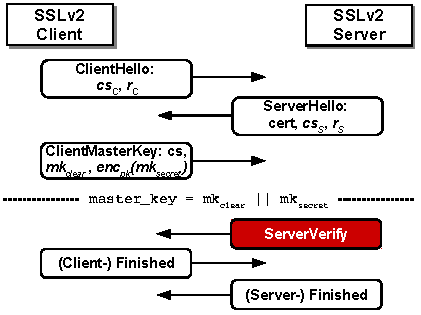
\includegraphics[width=\linewidth]{\DrownFigures/ssl-handshake} 
	\caption{\textbf{\ssltwo handshake.} The server responds with a \texttt{ServerVerify} message directly after receiving an RSA-\PKCS ciphertext contained in \texttt{ClientMasterKey}. This protocol feature enables our attack.\looseness=-1}
	\label{fig:ssl-handshake}
\end{figure}
%\fi
%
A client initiates an \ssltwo handshake by sending a
\texttt{ClientHello} message, which includes a list of cipher
suites $cs_c$ supported by the client and a client nonce $r_c$,
termed \texttt{challenge}.
The server responds with a \texttt{ServerHello} message, which
contains a list of cipher suites $cs_s$ supported by the server,
the server certificate, and a server nonce $r_s$, termed
$\texttt{connection\_ID}$.

The client responds with a \texttt{ClientMasterKey} message, which
specifies a cipher suite supported by both peers and key data
used for constructing a \texttt{master\_key}. In order to support
\textit{export} cipher suites with 40-bit security (e.g.,
\texttt{SSL\_RC2\_128\_CBC\_EXPORT40\_WITH\_MD5}), the key data is
divided into two parts:
\begin{itemize}
	\item $mk_{clear}$: A portion of the \texttt{master\_key} sent in the \texttt{ClientMasterKey} message as plaintext (termed \texttt{clear\_key\_data} in the \ssltwo standard).
	\item $mk_{secret}$: A secret portion of the
          \texttt{master\_key}, encrypted with RSA \PKCS (termed \texttt{secret\_key\_data}). 
\end{itemize}
The resulting \texttt{master\_key} $mk$ is constructed by
concatenating these two keys: $mk = mk_{clear} || mk_{secret}$. For
40-bit export cipher suites, $mk_{secret}$ is five bytes in length.
For non-export cipher suites, the whole \texttt{master\_key} is
encrypted, and the length of $mk_{clear}$ is zero.

The client and server can then compute session keys from the reconstructed \texttt{master\_key} $mk$:

\vspace{-6pt}
\begin{center}
\begin{math}
	\texttt{server\_write\_key} = MD5(mk || ``0" || r_c || r_s) \linebreak	
	\texttt{client\_write\_key} = MD5(mk || ``1" || r_c || r_s)
\end{math}
\end{center}
\vspace{-6pt}

The server responds with a \texttt{ServerVerify} message
consisting of the \texttt{challenge} $r_c$ encrypted with the
\texttt{server\_write\_key}.  Both peers then exchange
\texttt{Finished} messages in order to authenticate to each other.

Our attack exploits the fact that the server always decrypts an RSA-\PKCS
ciphertext, computes the \texttt{server\_write\_key}, and \textit{immediately}
responds with a \texttt{ServerVerify} message.  The \ssltwo standard
implies this message ordering, but does not make it explicit.
However, we observed this behavior in every implementation we
examined.  Our attack also takes advantage of the fact that the
encrypted $mk_{secret}$ portion of the \texttt{master\_key} can vary
in length, and is only five bytes for export ciphers.

% I Merged SSLv2 description and key derivation, ther were some redundancies ...

%\subsubsection{The SSLv2 key derivation mechanism}
%
%Recall that the RSA decryption code on the server decrypts the received RSA ciphertext, and checks the validity of the resulting plaintext as per the PKCS \#1 format. If the plaintext is valid, the server extracts from it the unpadded data, and uses that data, along with other information exchanged thus far during the protocol run, as the key for the chosen symmetric cipher. More formally:
%
%\begin{itemize}
%	\item Let the data from the decrypted RSA plaintext, after padding is removed, be termed \texttt{secret\_key\_data}.
%	\item Recall that the client and server have already exchanged a client nonce, termed \texttt{challenge} in the protocol standard, and a server nonce, termed $\texttt{connection\_ID}$.
%	\item Assume, as is the case throughout this work, that the chosen symmetric cipher is either export RC4 with a 128-bit key, of which 40 bits are secret, or export RC2 with the same key sizes\footnote{details vary slightly, but are very similar for other ciphers}. Then the client should send, along with the RSA ciphertext, a portion of the symmetric key in cleartext, termed \texttt{clear\_key\_data}, where \texttt{clear\_key\_data} is 11 bytes long. The sent \texttt{secret\_key\_data} should be exactly 5 bytes long. Let $\texttt{master\_key} = \texttt{clear\_key\_data} | \texttt{secret\_key\_data}$, where in this context $|$ refers to the concatenation operator.
%	\item Now let
%
%$\texttt{server\_write\_key} = MD5(\texttt{master\_key} | "0" | \texttt{challenge} | \texttt{connection\_ID})$
%
%$\texttt{client\_write\_key} = MD5(\texttt{master\_key} | "1" | \texttt{challenge} | \texttt{connection\_ID})$
%
%where the $|$ operator again means concatenation, and "0" and "1" refer to the corresponding ascii characters.
%
%	\item The respective keys are then used by each party both as keys for the chosen symmetric cipher, and as MAC keys.
%\end{itemize}

%As was hinted in the previous subsection, once an RSA key exchange with PKCS \#1 is implemented, the question immediately arises of how to act given an invalid RSA plaintext - recall that any observable difference in the treatment of invalid messages exposes a Bleichenbacher oracle to the attacker.
%Most implementations, including openssl, employ a counter-mechanism that has become somewhat standard: If the RSA plaintext is invalid or is of a wrong length, generate a random sequence of bytes of the expected length, and treat that sequence of bytes as if that was the plaintext after padding removal.
%
%As an aside, we note this counter-mechanism entails the risk of a timing attack: If the random byte sequence generation takes a measurable amount of time, an attacker may be able to observe the difference in processing times, and deduce the validity of the plaintext. Therefore, this counter-mechanism should be carefully implemented so as to require constant processing time. This is usually done by generating the random byte sequence before the RSA decryption, and choosing between the random sequence and the RSA plaintext according to the validity of the PKCS \#1 formatting. In fact, openssl's implementation of this mechanism was originally not constant-time for SSLv2, but the implementation was appropriately changed after we drew the maintainers' attention to this problem.



\ifsubmit\relax\else
\begin{figure}
	%\centering 
	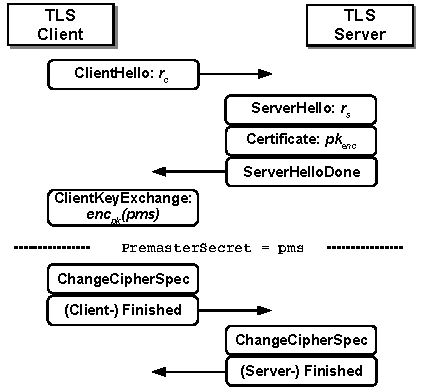
\includegraphics[width=\linewidth]{\DrownFigures/tls-handshake} 
	\caption{\textbf{TLS-RSA handshake.} After receiving an encrypted \pms, the server waits for an authenticated \texttt{ClientFinished} message.}
	\label{fig:tls-handshake}
\end{figure}
\fi

\paragraph{The TLS handshake protocol.}
In TLS~\cite{rfc5246} or \sslthree, the client initiates the handshake with a \texttt{ClientHello}, which contains a client random $r_c$ and a list of supported cipher suites. The server chooses one of the cipher suites and responds with three messages, \texttt{ServerHello}, \texttt{Certificate}, and \texttt{ServerHelloDone}. These messages include the server's choice of cipher suite, server nonce $r_s$, and a server certificate with an RSA public key. The client then uses the public key to encrypt a newly generated 48-byte \pms $pms$ and sends it to the server in a \texttt{ClientKeyExchange} message. The client and server then derive encryption and MAC keys from the \pms and the client and server random nonces. The details of this derivation are not important to our attack.  The client then sends \texttt{ChangeCipherSpec} and \texttt{Finished} messages. The \texttt{Finished} message authenticates all previous handshake messages using the derived keys. The server responds with its own \texttt{ChangeCipherSpec} and \texttt{Finished} messages.

The two main details relevant to our attacks are:
\begin{itemize}
	\item The \pms is always 48 bytes long, independent of the chosen cipher suite.  This is also true for export cipher suites.
	\item After receiving the \texttt{ClientKeyExchange} message, the server waits for the \texttt{ClientFinished} message, in order to authenticate the client.
\end{itemize}


\ifsubmit\relax\else
\subsubsection{Real-world protocol support}
TLSv1.0 is the most commonly supported protocol version, according to several surveys.  The SSL Labs SSL Pulse survey~\cite{ssllabs} reports that 98.6\% of about 140,000 popular TLS/SSL-enabled web sites supported TLSv1.0 in January 2016.  72.0\% supported TLSv1.2.  Support for \ssltwo was at 9.3\%, and \sslthree was at 29\%. Mayer et al.~\cite{DBLP:journals/corr/MayerZSH15} performed Internet-wide surveys of SMTP, IMAP, and POP3 between April and August 2015, and found that support for \ssltwo support was as high as 41.7\% of servers for SMTP on port 25 and as low as 3.7\% of IMAP servers on port 143.  Support for TLSv1.0 was nearly universal on these ports, varying from 91.6\% on port 25 to 98.9\% on port 143.

Bowen~\cite{bowencab} collected 213 million SSL/TLS client hellos and user agent strings from connections to popular sites, of which 183,000 (0.09\%) client hellos supported \ssltwo.  All of these client hellos also supported at least TLSv1.0.

Holz et al.~\cite{2016holz_analysis_tls-based_protocols_electronic_communication} performed passive monitoring to collect information about 16 million SSL/TLS connections during one week in July-August 2015.  They did not report any numbers for \ssltwo, and stated in personal communication that they did not observe any \ssltwo connections in their dataset.
\fi

%In response to our disclosure, OpenSSL has disabled \ssltwo by default in the 1.0.1r and 1.0.2f releases~\cite{opensslchangelog}.  

%This bug was also fixed in the aforementioned openssl releases.

\subsection{Bleichenbacher's attack}
\label{sec:bleichenbacher}
Bleichenbacher's attack is a padding oracle attack---it exploits the
fact that RSA ciphertexts should decrypt to \PKCS-compliant plaintexts.
If an implementation receives an RSA
ciphertext that decrypts to an invalid \PKCS plaintext, it might
naturally leak this information via an error message, by closing the
connection, or by taking longer to process the error condition.  This
behavior can leak information about the plaintext that can be modeled
as a cryptographic \textit{oracle} for the decryption
process. Bleichenbacher~\cite{Bleichenbacher} demonstrated how such an
oracle could be exploited to decrypt RSA ciphertexts.

%For example, the decrypting code may require different processing times for valid vs.\ invalid plaintexts - this is termed a "timing side-channel vulnerability". As another example, the decrypting code may send messages derived in some way from the plaintexts - this is termed a "direct message side channel vulnerability".
%The seminal work in this area \cite{Bleichenbacher} identified the general potential for such vulnerabilities, specifically using a direct message side channel vulnerability present in TLS implementations at the time, and demonstrated how such information could be gradually combined to eventually decrypt the RSA ciphertext in full.

\paragraph{Algorithm.}
In the simplest attack scenario, the attacker has a valid \PKCS
ciphertext $c_{0}$ that they wish to decrypt to discover the message
$m_{0}$.  They have no access to the private RSA key, but instead have
access to an oracle $\Oracle$ that will decrypt a ciphertext $c$ and
inform the attacker whether the most significant two bytes match
the required value for a correct \PKCS padding:
\begin{equation*} 
\Oracle(c) =  
\begin{cases} 
1 & \text{ if } m=c^d \bmod N \text{ starts with \hexb{00}{02}} \\ 
0 & \text{ otherwise.} 
\end{cases} 
\end{equation*} 

If the oracle answers with \texttt{1}, the attacker knows that $2B
\leq m \leq 3B-1$, where $B = 2^{8(\ell_m-2)}$.  The attacker can
take advantage of RSA malleability to generate new candidate ciphertexts
for any $s$:
\[
c = (c_{0} \cdot s^e) \bmod N = (m_{0} \cdot s)^e \bmod N 
\]
The attacker queries the oracle with $c$. If the oracle responds with
$0$, the attacker increments $s$ and repeats the previous
step. Otherwise, the attacker learns that for some~$r$, $2B \leq m_{0}s - rN  < 3B$. This allows the attacker to reduce the range of possible solutions to:  
\[ 
\frac{2B+rN}{s} \leq m_{0} < \frac{3B+rN}{s}  
\] 
The attacker proceeds by refining guesses for $s$ and $r$ values and
successively decreasing the size of the interval containing $m_{0}$.  At
some point the interval will contain a single valid value, $m_{0}$.
Bleichenbacher's original paper describes this process in further
detail~\cite{Bleichenbacher}.

\paragraph{Countermeasures.}
In order to protect against this attack, the decrypter must not leak
information about the \PKCS validity of the ciphertext.  The
ciphertext does not decrypt to a valid message, so the
decrypter generates a fake plaintext and continues the
protocol with this decoy.  The attacker should not be able to
distinguish the resulting computation from a correctly decrypted
ciphertext.

In the case of SSL/TLS, the server generates a random \pms to continue
the handshake if the decrypted ciphertext is
invalid.  The client will not possess the session key to send a valid
\texttt{ClientFinished} message and the connection will terminate.



%\input{libraries}

% !TEX root = subgroup.tex
\ApplicationsTable

\section{TLS}\label{sec:tls}

TLS (Transport Layer Security) is a transport layer protocol designed to provide confidentiality,
integrity and (most commonly) one-side authentication for application sessions. 
It is widely used to protect HTTP and mail protocols. 

A TLS client initiates a TLS handshake with the \texttt{Client\-Hello} message.
This message includes a list of supported cipher suites, and a client random
nonce $r_c$. The server responds with a \texttt{Server\-Hello} message containing
the chosen cipher suite and server random nonce $r_s$, and a
\texttt{Certificate} message that includes the server's X.509 certificate. If
the server selects a cipher suite using ephemeral Diffie-Hellman key exchange,
the server additionally sends a \texttt{Server\-Key\-Exchange} message containing
the server's choice of Diffie-Hellman parameters $p$ and $g$, the server's
Diffie-Hellman public value $y_s = g^{x_s} \bmod p$, a signature by the
server's private key over both the client and server nonces ($r_c$ and $r_s$),
and the server's Diffie-Hellman parameters ($p$, $g$, and $y_s$). The client
then verifies the signature using the public key from the server's certificate,
and responds with a \texttt{Client\-Key\-Exchange} message containing the client's
Diffie-Hellman public value $y_c = g^{x_c} \bmod p$. The Diffie-Hellman shared
secret $Y = g^{x_s x_c} \bmod p$ is used to derive encryption and MAC keys. The
client then sends \texttt{Change\-Cipher\-Spec} and \texttt{Finished} messages. The
\texttt{Finished} message contains a hash of the handshake transcript, and is
encrypted and authenticated using the derived encryption and MAC keys. Upon
decrypting and authenticating this message, the server verifies that the hash
of the transcript matches the expected hash.  Provided the hash matches, the
server then sends its own \texttt{Change\-Cipher\-Spec} and \texttt{Finished}
messages, which the client then verifies. If either side fails to decrypt or
authenticate the \texttt{Finished} messages, or if the transcript hashes do not
match, the connection fails immediately~\cite{rfc5246}.

TLS also specifies a mode of using Diffie-Hellman with fixed parameters from
the server's certificate~\cite{rfc3279}. This mode is not forward secret, was
never widely adopted, and has been removed from all modern browsers due to
dangerous protocol flaws~\cite{kci-tls-2015}. The only widely used form of
Diffie-Hellman in TLS today is ephemeral Diffie-Hellman, described above.

\subsection{Small Subgroup Attacks in TLS}
\label{sec:tls-subgroup-attack}

\paragraph{Small subgroup confinement attacks}
A malicious TLS server can perform a variant of the small subgroup attack
against a client by selecting group parameters $g$ and $p$ such that $g$
generates an insecure group order. TLS versions prior to 1.3 give the server
complete liberty to choose the group, and they do not include any method for
the server to specify the desired group order $q$ to the client.  This means a
client has no feasible way to validate that the group sent by the server has the
desired level of security or that a server's key exchange value is in
the correct group for a non-safe prime.
\looseness=-1

Similarly, a man in the middle with knowledge of the server's long-term private
signing key can use a small subgroup confinement attack to more easily
compromise perfect forward secrecy, without having to rewrite an entire
connection. The attack is similar to the those described by Bhargavan and
Delignat-Lavaud~\cite{bhargavan-channel-bindings-2015}. The attacker modifies the
server key exchange message, leaving the prime unchanged, but substituting a
generator $g_i$ of a subgroup of small order $q_i$ for the group generator and 
$g_i$ for the server's key exchange value $y_s$. The attacker then forges a correct signature for the modified server key exchange message and passes it to the client.  The client then
responds with a client key exchange message $y_c = g_i^{x_c} \bmod p$, which
the man-in-the-middle leaves unchanged. The server's view of the shared secret
is then $g_i^{x_c x_s} \bmod p$, and the client's view of the shared secret is
$g_i^{x_c} \bmod p$. These views are identical when ${x_s} \equiv 1 \bmod q_i$,
so this connection will succeed with probability $1/q_i$. For small enough
$q_i$, this enables a man in the middle to use a compromised server signing key to
decrypt traffic from forward-secret ciphersuites with a reasonable probability
of success, while only requiring tampering with a single handshake message,
rather than having to actively rewrite the entire connection for the duration of the session.

Furthermore, if the server uses a static Diffie-Hellman key exchange value,
then the attacker can perform a small subgroup key-recovery attack as the
client in order to learn the server's static exponent $x_s \bmod q_i$ for the
small subgroup. This enables the attacker to calculate a custom generator such
that the client and server views of the shared secret are always identical,
raising the above attack to a 100\% probability of success.

\TLSLibraryTable

\paragraph{Small subgroup key recovery attacks} In TLS, the client must
authenticate the handshake before the server, by providing a valid
\texttt{Finished} message. This forces a small subgroup key recovery attack
against TLS to be primarily online. To perform a Lim-Lee small subgroup key
recovery attack against a server static exponent, a malicious client initiates
a TLS handshake and sends a generator $g_i$ of a small subgroup of order $q_i$
as its client key exchange message $y_c$.  The server will calculate $Y_s =
g_i^{x_s} \bmod p$ as the shared secret. The server's view of the shared secret
is confined to the subgroup of order $q_i$.  However, since $g_i$ and $g$
generate separate subgroups, the server's public value $y_s = g^x_s$ gives the
attacker no information about the value of the shared secret $Y_s$. Instead,
the attacker must guess a value for $x_s \bmod q_i$, and send the corresponding
client \texttt{Finished} message. If the server continues the handshake, the
attacker learns that the guess is correct.  Therefore, assuming the server is
reusing a static value for $x_s$, the attacker needs to perform at most $q_i$
queries to learn the  server's secret $x_s \bmod q_i$~\cite{lim-1997}. This
attack is feasible if $q_i$ is small enough and the server reuses
Diffie-Hellman exponents for sufficiently many requests.

The attacker repeats this process for many different primes $q_i$, and uses the
Chinese remainder theorem to combine them modulo the product of the primes
$q_i$.  The attacker can also use the Pollard lambda algorithm to reconstruct
any remaining bits of the exponent~\cite{lim-1997}.



We note that the TLS False Start extension allows the
server to send application data before receiving the client's authentication~\cite{rfc7918}.
The specification only allows this behavior for abbreviated handshakes, which
do not include a full key exchange.  If a full key exchange were allowed, the
fact that the server authenticates first would allow a malicious client to
mount a mostly offline key recovery attack.
%\todo{Add discussion of the old unused TLS extension that makes this offline. \ref{rfc7918}}



\subsection{OpenSSL}

Prior to early 2015, OpenSSL defaulted to using static-ephemeral Diffie-Hellman
values. Server applications generate a fresh Diffie-Hellman secret exponent on
startup, and reuse this exponent until they are restarted.  A server would be
vulnerable to small subgroup attacks if it chose a DSA prime, explicitly
configured the \texttt{dh->length} parameter to generate a short exponent, and
failed to set \texttt{SSL\_OP\_SINGLE\_DH\_USE} to prevent repeated exponents.
OpenSSL provides some test code for key generation which configures DSA group
parameters, sets an exponent length to the group order, and correctly sets the
\texttt{SSL\_OP\_SINGLE\_DH\_USE} to generate new exponents on every
connection.  We found this test code widely used across many applications.  We
discovered that Unbound, a DNS resolver, used the same parameters as the tests,
but without setting \texttt{SSL\_OP\_SINGLE\_DH\_USE}, rendering them
vulnerable to a key recovery attack.  A number of other applications including
Lighttpd used the same or similar code with non-safe primes, but correctly set
\texttt{SSL\_OP\_SINGLE\_DH\_USE}.

In spring 2015, OpenSSL added explicit support for RFC~5114
groups~\cite{openssl-changelog-102}, including the ability for servers to
specify a subgroup order in a set of Diffie-Hellman group parameters. When the
subgroup order is specified, the exponent length is automatically adjusted to
match the subgroup size.  However, the update did not contain code to validate
subgroup order for key exchange values, leaving OpenSSL users vulnerable to
precisely the key recovery attack outlined in
Section~\ref{sec:tls-subgroup-attack}.

We disclosed this vulnerability to OpenSSL in January 2016. The vulnerability
was patched by including code to validate subgroup order when a subgroup was
specified in a set of Diffie-Hellman parameters and setting
\texttt{SSL\_OP\_SINGLE\_DH\_USE} by default~\cite{openssl-secadv-subgroup}.
Prior to this patch, any code using OpenSSL for DSA-style Diffie-Hellman
parameters was vulnerable to small subgroup attacks by default.

Exim~\cite{exim}, a popular mail server that uses OpenSSL, provides a clear
example of the fragile situation created by this update. By default, Exim uses
the RFC~5114 Group 23 parameters with OpenSSL, does not set an exponent length,
and does not set \texttt{SSL\_OP\_SINGLE\-\_DH\_USE}. In a blog post, an Exim
developer explains that because of ``numerous issues with automatic generation
of DH parameters'', they added support for fixed groups specified in RFCs and picked
Group~23 as the default~\cite{exim-blog}.  Exim narrowly avoided being fully
vulnerable to a key recovery attack by not including the size of the subgroup
generated by $q$ in the Diffie-Hellman parameters that it passes to OpenSSL.
Had this been included, OpenSSL would have automatically shortened the exponent
length, leaving the server fully vulnerable to a key recovery attack.  For this
group, an attacker can recover 130 bits of information about the secret
exponent using $2^{33}$ online queries, but this does not allow the attacker to
recover the server's 2048-bit exponent modulo the correct 224-bit group order
$q$ as the small subgroup orders $q_i$ are all relatively prime to $q$.

We looked at several other applications as well, but did not find them to be
vulnerable to key recovery attacks (Table~\ref{tab:common-applications}).



% comprising 53.62\% of all such servers~\cite{esoft2016}.

% Exim can be compiled either with GNU TLS or with OpenSSL. When compiled with OpenSSL,
% it supports single use DH keys with an option that is off by default
% (as of version 4.87, the latest at time of writing). In OpenSSL mode, it
% includes checks for unsafe primes and incorrect generators, however it
% ignores the generator check when the generator is not 2 or 5, due to a known
% bug in OpenSSL. More significantly, it utilizes the DSA primes with small
% subgroups. Their code comments note ``These have been thoroughly reviewed as
% meeting certain eligibility criteria, which is more than can be said for primes
% generated quickly''. However, they fail to note the difference in criteria for
% the DSA primes as opposed to the others, resulting in the selection of vulnerable
% groups. The subgroup size $q$ was not included in the Exim's default DSA parameter, saving 
% a default Exim installation from being vulnerable to the attack described 
% in Section~\ref{sec:tls-subgroup-attack} due the fact that OpenSSL did not have the possibility 
% to match the exponent length to subgroup size. Said that, if the DSA parameter would have been generated using the 
% OpenSSL's genpkey utility~\cite{genpkey} all the conditions to perform the Small subgroup key recovery attack
% as per Section ~\ref{sec:tls-subgroup-attack} would have been met.
% In comparison Postfix an MX  utilized for 32.80\% of mail servers~\cite{esoft2016}
% suggests generating a group at install time but neglects to set the single use OpenSSL option
% and includes two hardcoded groups by default.



\ScanTable

\subsection{Other Implementations} \label{subsec:nss}

We examined the source code of multiple TLS implementations
(Table~\ref{tab:tls-implementations}). Prior to January 2016, no TLS
implementations that we examined validated group order, even for the well-known
DSA primes from RFC~5114, leaving them vulnerable to small subgroup confinement attacks.

Most of the implementations we examined attempt to match exponent length to the
perceived strength of the prime. For example, Mozilla Network Security Services
(NSS), the TLS library used in the Firefox browser and some versions of
Chrome~\cite{nss-overview,chrome-to-openssl}, uses NIST's ``comparable key strength'' recommendations
on key management~\cite{sp800} to determine secret exponent lengths from the length of the prime.~\cite{nss-line-of-code}  Thus NSS uses 160-bit exponents with a 1024-bit prime, and 224-bit exponents with a 2048-bit prime.
 In fall 2015, NSS added an additional check to ensure that the
shared secret $g^{x_ax_b} \not \equiv 1 \bmod p$~\cite{nss-code-secret-not-one}.

Several implementations go to elaborate lengths to match exponent length to
perceived prime strength.  The Cryptlib library fits a quadratic curve to the
small exponent attack cost table in the original van~Oorschot
paper~\cite{van1996diffie} and uses the fitted curve to determine safe key
lengths~\cite{cryptlib-fitted-curve}. The Crypto++ library uses an explicit
``work factor'' calculation, evaluating the function $2.4 n^{1/3} (\log
n)^{2/3}$~\cite{cryptoplusplus-work-factor}. Subgroup order and exponent
lengths are set to twice the calculated work factor. The work factor
calculation is taken from a 1995 paper by Odlyzko on integer
factorization~\cite{odlyzko-1995}. Botan, a C++ cryptography and TLS library,
uses a similar work factor calculation, derived from RFC~3766~\cite{rfc3766},
which describes best practices as of 2004 for selecting public key strengths
when exchanging symmetric keys. RFC~3766 uses a similar work factor algorithm
to Odlyzko, intended to model the running time of the number-field
sieve. Botan then doubles the length of the work factor to obtain subgroup and
exponent lengths~\cite{botan-double}.

% Apple Safari on OS X and iOS performed no validation of
% Diffie-Hellman prime lengths until July 2015, and supported connections where
% the server offered a trivially-broken group using a 16-bit prime~\cite{weakdh-ccs15}.

\subsection{Measurements}
\label{sec:tls-measurements}

We used ZMap~\cite{zmap-2013} to probe the public IPv4 address space for hosts
serving three TLS-based protocols: HTTPS, SMTP+STARTTLS, and POP3S\@.  To
determine which primes servers were using, we sent a \texttt{ClientHello}
message containing only ephemeral Diffie-Hellman cipher suites.  We combined
this data with scans from Censys~\cite{censys} to determine the overall
population.  The results are summarized in Table~\ref{tab:scandata}. 

\TLSHostValidationTable

\PrimesAllTLS

In August 2016, we conducted additional scans of a random 1\% sample
of HTTPS hosts on the Internet.  First, we checked for nontrivial
small subgroup attack vulnerability. For servers that sent us a prime
$p$ such that $p-1$ was divisible by 7, we attempted a handshake using
a client key exchange value of $g_7\bmod p$, where $g_7$ is a
generator of a subgroup of order $7$.  (7 is the smallest prime factor
of $p-1$ for Group 22.) When we send $g_7$, we expect to correctly
guess the \texttt{PreMasterSecret} and complete the handshake with one
seventh of hosts that do not validate subgroup order. In our scan, we
were able to successfully complete a handshake with $1477$ of $10714$
hosts that offered a prime such that $p-1$ was divisible by $7$,
implying that approximately 96\% of these hosts fail to validate
subgroup order six months after OpenSSL pushed a patch adding group
order validation for correctly configured groups.

Second, we measured how many hosts performed even the most basic
validation of key exchange values. We attempted to connect to HTTPS hosts with
the client key exchange values of $y_c = 0 \bmod p, 1 \bmod p, -1 \bmod p$. As
Table~\ref{tab:tlsvalidation} shows, we found that over 5\% of hosts that
accepted DHE ciphersuites accepted the key exchange value of $-1 \bmod p$ and
derived the \texttt{PreMasterSecret} from it. These implementations are
vulnerable to a trivial version of the small subgroup confinement attacks
described in Section~\ref{sec:tls-subgroup-attack}, for \emph{any} prime
modulus $p$. By examining the default web pages of many of these hosts,
we identified products from several notable companies including Microsoft,
Cisco, and VMWare. When we disclosed these findings, VMWare notified us that
they had already applied the fix in the latest version of their products;
Microsoft acknowledged the missing checks but chose not to include them since
they only use safe primes, and adding the checks may break functionality
for some clients that were sending unusual key exchange values; and Cisco
informed us that they would investigate the issue.

Of 40.6\,M total HTTPS hosts found in our scans, 10.8\,M~(27\%) supported
ephemeral Diffie-Hellman, of which 1.6\,M~(4\%) used a non-safe prime, and
309\,K~(0.8\%) used a non-safe prime and reused exponents across multiple
connections, making them likely candidates for a small subgroup key recovery
attack.  We note that the numbers for hosts reusing exponents are an
underestimate, since we only mark hosts as such if we found them using the same
public Diffie-Hellman value across multiple connections, and some load
balancers that cycle among multiple values might have evaded detection.

While 77\%~of POP3S hosts and 39\%~of SMTP servers used a non-safe prime, a
much smaller number used a non-safe prime and reused exponents (<0.01\% in both
protocols), suggesting that the popular implementations (Postfix and
Dovecot~\cite{mail-2015}) that use these primes follow recommendations to use
ephemeral Diffie-Hellman values with DSA primes.

Table~\ref{tab:primes} shows nine groups that accounted for the majority of
non-safe primes used by hosts in the wild. Over 1.17\,M hosts across all of our
HTTPS scans negotiated Group~22 in a key exchange. To get a better picture of
which implementations provide support for this group, we examined the default
web pages of these hosts to identify companies and products, which we show in
Table~\ref{tab:tls-group22-support}.

\TLSGroupSupport


Of the the 307\,K HTTPS hosts that both use non-safe primes and reuse
exponents, 277\,K~(90\%) belong to hosts behind Amazon's Elastic Load
Balancer~\cite{amazon-elb}. These hosts use a 1024-bit prime with a 160-bit
subgroup. We set up our own load balancer instance and found that the
implementation failed to validate subgroup order. We were able to use a
small-subgroup key recovery attack to compute 17 bits of our load balancer's
private Diffie-Hellman exponent $x_s$ in only 3813 queries.  We responsibly
disclosed this vulnerability to Amazon. Amazon informed us that they have
removed Diffie-Hellman from their recommended ELB security policy, and are
encouraging customers to use the latest policy.  In May 2016, we performed
additional scans and found that 88\% of hosts using this prime no longer
repeated exponents.   We give a partial factorization for $p-1$ in
Table~\ref{tab:group-order-factorization}; the next largest subgroups have 61
and 89 bits and an offline attack against the remaining bits of a 160-bit
exponent would take $2^{71}$ time.  For more details on the computation, see
Section~\ref{sec:ecm}.

SSLeay~\cite{ssleay}, a predecessor for OpenSSL, includes several default
Diffie-Hellman primes, including a 512-bit prime. We found that 717 SMTP
servers used a version of the OpenSSL 512-bit prime with a single character
difference in the hexadecimal representation.  The resulting modulus that these
servers use for their Diffie-Hellman key exchange is no longer prime. We
include the factorization of this modulus along with the factors of the
resulting group order in Table~\ref{tab:group-order-factorization}. The use of
a composite modulus further decreases the work required to perform a small
subgroup attack.

Although TLS also includes static Diffie-Hellman cipher suites that require a
DSS certificate, we did not include them in our study; no browser supports
static Diffie-Hellman~\cite{kci-tls-2015}, and Censys shows no hosts with DSS
certificates, with only 652 total hosts with non-RSA or ECDSA certificates.

%In February 2016, we conducted an additional scan of a random 1\% sample of the
%Internet to check how many hosts performed even the most basic validation of
%key exchange values. We attempted to connect to HTTPS hosts with a client
%key exchange message of $y_c = 1$. We found that 322 of 589,241 hosts accepted
%this key exchange value and derived the \texttt{PreMasterSecret} from it. 248
%of these hosts were Cisco devices, another 28 were VMware Horizon View servers,
%and the remaining 46 devices did not fit into any clear category. These
%implementations are vulnerable to a trivial version of the small subgroup
%confinement attacks described in Section~\ref{sec:tls-subgroup-attack}.\todo{did we disclose this? we need to. also what about validation of values other than 0?}


%\TODO{classify implementations again and disclose to Cisco, etc}








% !TEX root = ../../../proposal.tex

\section{IPsec}

%Description of IKEv1 and IKEv2.

IPsec is a set of Layer-3 protocols which add confidentiality, data protection,
sender authentication, and access control to IP traffic. IPsec is commonly used
to implement VPNs.
%IPsec provides two types of security service: Authentication Header (AH),
%which provides sender authentication, and Encapsulating Security Payload
%(ESP), which provides both sender authentication and payload encryption.  Each
%of these services requires the communicating parties to establish shared
%state, which includes the cryptographic algorithms used to provide the service
%and the keys used as input for the cryptographic algorithms.
IPsec uses the Internet Key Exchange (IKE) protocol to determine the keys used
to secure a session. IPsec may use IKEv1~\cite{rfc2409} or
IKEv2~\cite{rfc7296}. While IKEv2 is not backwards-compatible with IKEv1, the
two protocols are similar in message structure and purpose. Both versions use
Diffie-Hellman to negotiate shared secrets. The groups used are limited to a
fixed set of pre-determined choices, which include the DSA groups from
RFC~5114, each assigned a number by IANA~\cite{rfc3526,rfc5114,rfc7296}.

% IKE versions
\paragraph{IKEv1}
%IKEv1 is a hybrid protocol built upon three other protocols:
%ISAKMP~\cite{rfc2408}, which establishes a framework for authentication and
%key exchange; Oakley~\cite{rfc2412}, which defines a series of key exchanges
%and services based on the Diffie-Hellman key exchange; and
%SKEME~\cite{krawczyk1996skeme}, a key exchange protocol that provides
%anonymity, repudiability, and quick key refreshement.  IKEv1 is formally
%defined in RFCs 2407~\cite{rfc2407}, 2408~\cite{rfc2408}, and
%2409~\cite{rfc2409}. 
IKEv1~\cite{rfc2407,rfc2408,rfc2409} has two basic methods for authenticated
key exchange: Main Mode and Aggressive Mode. Main Mode requires six messages to
establish the requisite state. The initiator sends a Security Association
(\texttt{SA}) payload, containing a selection of cipher suites and
Diffie-Hellman groups they are willing to negotiate. The responder selects a
cipher and responds with its own \texttt{SA} payload. After the cipher suite is
selected, the initiator and responder both transmit Key Exchange (\texttt{KE})
payloads containing public Diffie-Hellman values for the chosen group. At this
point, both parties compute shared key materials, denoted \texttt{SKEYID}. When
using signatures for authentication, \texttt{SKEYID} is computed
$\texttt{SKEYID} = \operatorname{prf}(N_i | N_r, g^{x_ix_r})$.  For the other
two authentication modes, pre-shared key and public-key encryption,
\texttt{SKEYID} is derived from the pre-shared key and session cookies,
respectively, and does not depend on the negotiated Diffie-Hellman shared
secret.

Each party then in turn sends an authentication message (\texttt{AUTH}) derived
from a hash over \texttt{SKEYID} and the handshake. The authentication messages
are encrypted and authenticated using keys derived from the Diffie-Hellman
secret $g^{x_i x_r}$.  The responder only sends her \texttt{AUTH} message after
receiving and validating the initiator's \texttt{AUTH} message.

Aggressive Mode operates identically to Main Mode, but in order to reduce
latency, the initiator sends \texttt{SA} and \texttt{KE} messages together, and
the responder replies with its \texttt{SA}, \texttt{KE}, and \texttt{AUTH}
messages together. In aggressive mode, the responder sends an authentication
message first, and the authentication messages are not encrypted.


\paragraph{IKEv2}
%IKE Version 2 (IKEv2) was released in RFC 4306~\cite{rfc4306} to replace IKEv1
%and the plethora of RFCs that define it. RFC 7296~\cite{rfc7296} gives the
%current version of the IKEv2 specification.
IKEv2~\cite{rfc4306,rfc7296} combines the \texttt{SA} and \texttt{KE} messages
into a single message. The initiator provides a best guess ciphersuite for the
\texttt{KE} message. If the responder accepts that proposal and chooses not to
renegotiate, the responder replies with a single message containing both
\texttt{SA} and \texttt{KE} payloads. Both parties then send and verify
\texttt{AUTH} messages, starting with the initiator.  The authentication
messages are encrypted using session keys derived from the \texttt{SKEYSEED}
value which is derived from the negotiated Diffie-Hellman shared secret. The
standard authentication modes use public-key signatures over the handshake
values.

%IKE Group~23, the 2048-bit MODP group with a 224-bit subgroup, is particularly
%vulnerable as shown in Section~\ref{sec:ecm}.

\subsection{Small Subgroup Attacks in IPsec} There are several variants of
small subgroup attacks against IKEv1 and IKEv2.  We describe the attacks
against these protocols together in this section.

\paragraph{Small subgroup confinement attacks} First, consider attacks that can
be carried out by an attacking initiator or responder. In IKEv1 Main Mode and
in IKEv2, either peer can carry out a small subgroup confinement attack against
the other by sending a generator of a small subgroup as its key exchange value.
The attacking peer must then guess the other peer's view of the Diffie-Hellman
shared secret to compute the session keys to encrypt its authentication
message, leading to a mostly online attack. However, in IKEv1 Aggressive Mode,
the responder sends its \texttt{AUTH} message before the initiator, and this
value is not encrypted with a session key. If signature authentication is being
used, the \texttt{SKEYID} and resulting hashes are derived from the
Diffie-Hellman shared secret, so the initiator can perform an offline
brute-force attack against the responder's authentication message to learn
their exponent in the small subgroup.

Now, consider a man-in-the-middle attacker. Bhargavan, Delignat-Lavaud, and
Pironti~\cite{bhargavan-channel-bindings-2015} describe a transcript synchronization
attack against IKEv2 that relies on a small subgroup confinement attack.  A
man-in-the-middle attacker initiates simultaneous connections with an initiator
and a responder using identical nonces, and sends a generator $g_i$ for a
subgroup of small order $q_i$ to each as its \texttt{KE} message.  The two
sides have a $1/q_i$ chance of negotiating an identical shared secret, so an
authentication method depending only on nonces and shared secrets could be
forwarded, and the session keys would be identical.

If the attacker also has knowledge of the secrets used for authentication, more
attacks are possible.  Similar to the attack described for TLS, such an
attacker can use a small subgroup confinement attack to force a connection to
use weak encryption. The attacker only needs to rewrite a small number of
handshake messages; any further encrypted communications can then be decrypted
at leisure without requiring the man-in-the-middle attacker to continuously
rewrite the connection. We consider a man-in-the-middle attacker who modifies
the key exchange message from both the initiator and the responder to
substitute a generator $g_i$ of a subgroup of small order $q_i$.  The attacker
must then replace the handshake authentication messages, which would require
knowledge of the long-term authentication secret.  We describe this attack for
each of pre-shared key, signatures, and public-key authentication. 

For pre-shared key authentication in IKEv1 Main Mode, IKEv1 Aggressive Mode,
and IKEv2, the man-in-the-middle attacker must only know the pre-shared key to
construct the authentication hash; the authentication message does not depend
on the negotiated Diffie-Hellman shared secret. With probability $1/q_i$, the
two parties will agree on the Diffie-Hellman shared secret. The attacker can
then brute force this value after viewing messages encrypted with keys derived
from it.

For signature authentication in IKEv1 Main Mode and in IKEv2, the signed hash
transmitted from each side is derived from the nonces and the negotiated shared
secret, which is confined to one of $q_i$ possible values.  The attacker must
know the private signing keys for both initiator and responder and brute force
\texttt{SKEYID} from the received signature in order to forge the modified
authentication signatures on each side. The communicating parties will have a
$q_i$ chance of agreeing on the same value for the shared secret to allow the
attack to succeed. For IKEv1 Aggressive Mode, the attack can be made to succeed
every time. The responder's key exchange message is sent together with their
signature which depends on the negotiated shared secret, so the
man-in-the-middle attacker can brute force the $q_i$ possible values of the
responders private key $x_r$ and replace the responder's key exchange message
with $q_i^{x_r}$, forging an appropriate signature with their knowledge of the
signing key.

For public key authentication in IKEv1 Main Mode, IKEv1 Aggressive Mode, and
IKEv2, the attacker must know the private keys corresponding to the public keys
used to encrypt the ID and nonce values on both sides in order to forge a valid
authentication hash.  Since the authentication does not depend on the shared
Diffie-Hellman negotiated value, a man-in-the-middle attacker must then brute
force the negotiated shared key once they receives a message encrypted with the
derived key.  The two parties will agree on their view of the shared key with
probability $1/q_i$, allowing the attack to succeed.

\paragraph{Small subgroup key recovery attacks} Similar to TLS, an IKE
responder that reuses private exponents and does not verify that the initiator
key exchange values are in the correct subgroup is vulnerable to a small
subgroup key recovery attack. The most recent version of the IKEv2
specification has a section discussing reuse of Diffie-Hellman exponents,
and states that ``because computing Diffie-Hellman exponentials is
computationally expensive, an endpoint may find it advantageous to reuse those
exponentials for multiple connection setups''~\cite{rfc7296}. Following this
recommendation could leave a host open to a key recovery attack, depending on
how exponent reuse is implemented. A small subgroup key recovery attack on IKE
would be primarily offline for IKEv1 with signature authentication and for
IKEv2 against the initiator.

For each subgroup of order $q_i$, the attacker's goal is to obtain a responder
\texttt{AUTH} message, which depends on the secret chosen by the responder. If
an \texttt{AUTH} message can be obtained, the attacker can brute-force the
responder's secret within the subgroup offline. This is possible if the server
supports IKEv1 Aggressive Mode, since the server authenticates before the
client, and signature authentication produces a value dependent on the
negotiated secret.  In all other IKE modes, the client authenticates first,
leading to an online attack. The flow of the attack is identical to TLS; for
more details see Section~\ref{sec:tls}.

Ferguson and Schneier~\cite{ferguson2000cryptographic} describe a hypothetical
small-subgroup attack against the initiator where a man-in-the-middle attacker
abuses undefined behavior with respect to UDP packet retransmissions. A
malicious party could ``retransmit'' many key exchange messages to an initiator
and potentially receive a different authentication message in response to each,
allowing a mostly offline key recovery attack.

%The attacker must choose their key exchange value to be a generator of the
%selected subgroup, which we call $g_i$.  When the responder computes the
%shared secret, $g_i^a$, it will lie within the chosen subgroup.  The attacker
%must guess $g_i^a \bmod q_i$, and construct their \texttt{AUTH} message
%accordingly.  The responder will reply with an \texttt{AUTH} message in the
%event of a correct guess, and an error message otherwise.  With repeated
%guessing, the attacker can learn the value of $g_i^a$ for each subgroup, and
%take advantage of the Pollard labmda algorithm to solve for the rest of the
%secret offline within the reduced search space.

\subsection{Implementations}

We examined several open-source IKE implementations to understand server
behavior.  In particular, we looked for implementations that generate small
Diffie-Hellman exponents, repeat exponents across multiple connections, or do
not correctly validate subgroup order. Despite the suggestion in IKEv2 RFC 7296
to reuse exponents~\cite{rfc7296}, none of the implementations that we examined
reused secret exponents. 

% This is already included in the intro
%RFC 6989~\cite{rfc6989} (``Additional Diffie-Hellman Tests for IKEv2'')
%specifies additional checks that IKE implementations supporting MODP groups
%with small subgroups should perform. The RFC requries IKE implementations to
%choose between either checking that the peer's public value is in the correct
%subgroup, or it must never reuse Diffie-Hellman private values. 

All implementations we reviewed are based on FreeS/WAN~\cite{freeswan}, a
reference implementation of IPSec. The final release of FreeS/Wan, version
2.06, was released in 2004. Version 2.04 was forked into
Openswan~\cite{openswan} and strongSwan\cite{strongswan}, with a further fork
of Openswan into Libreswan~\cite{libreswan} in 2012.  The final release of
FreeS/WAN used constant length 256-bit exponents but did not support RFC~5114
DSA groups, offering only the Oakley 1024-bit and 1536-bit groups that use safe
primes.

\IKEGroupSupportAndValidationTable

Openswan does not generate keys with short exponents. By default, RFC~5114
groups are not supported, although there is a compile-time option that can be
explicitly set to enable support for DSA groups.  strongSwan both supports
RFC~5114 groups and has explicit hard-coded exponent sizes for each group. The
exponent size for each of the RFC~5114 DSA groups matches the subgroup size.
However, these exponent sizes are only used if the
\texttt{dh\_exponent\_ansi\_x9\_42} configuration option is set. It also
includes a routine inside an \texttt{\#ifdef} that validates subgroup order by
checking that $g^q \equiv 1 \bmod p$, but validation is not enabled by default.
Libreswan uses Mozilla Network Security Services (NSS)~\cite{nss-overview} to
generate Diffie-Hellman keys. As discussed in Section~\ref{subsec:nss}, NSS
generates short exponents for Diffie-Hellman groups. Libreswan was forked from
Openswan after support for RFC~5114 was added, and retains support for those
groups if it is configured to use them. 

Although none of the implementations we examined were configured to reuse
Diffie-Hellman exponents across connections, the failure to validate subgroup
orders even for the pre-specified groups renders these implementations fragile
to future changes and vulnerable to subgroup confinement attacks.

Several closed source implementations also provide support for RFC~5114
Group~24. These include Cisco's IOS~\cite{ciscogroup24}, Juniper's
Junos~\cite{junosgroup24}, and Windows Server 2012 R2~\cite{windowsgroup24}. We
were unable to examine the source code for these implementations to determine
whether or not they validate subgroup order.

%\IKEGroupSupportAndValidationTable

\subsection{Measurements}

We performed a series of Internet scans using ZMap to identify IKE responders.
In our analysis, we only consider hosts that respond to our ZMap scan probes.
Many IKE hosts that filter their connections based on IP are excluded from our
results.  We further note that, depending on VPN server configurations, some
responders may continue with a negotiation that uses weak parameters until they
are able to identify a configuration for the connecting initiator. At that
point, they might reject the connection. As an unauthenticated initiator, we
have no way of distinguishing this behavior from the behaviour of a VPN server
that legitimately accepts weak parameters. For a more detailed explanation of
possible IKE responder behaviors in response to scanning probes, see
Wouters~\cite{paul-wouters}.

In October 2016, we performed a series of scans offering the most common cipher
suites and group parameters we found in implementations to establish a baseline
population for IKEv1 and IKEv2 responses. For IKEv1, the baseline scan offered
Oakley groups 2 and 14 and RFC~5114 groups 22, 23, and 24 for the group
parameters; SHA1 or SHA256 for the hash function; pre-shared key or RSA
signatures for the authentication method; and AES-CBC, 3DES, and DES for the
encryption algorithm.  Our IKEv2 baseline scan was similar, but also offered
the 256-bit and 384-bit ECP groups and AES-GCM for authenticated encryption.

On top of the baseline scans, we performed additional scans to measure support
for the non-safe RFC~5114 groups and for key exchange parameter validation.
Table~\ref{tab:ikegroupsupportandvalidation} shows the results of the October
IKE scans.  For each RFC~5114 DSA group, we performed four handshakes with each
host; the first tested for support by sending a valid client key exchange
value, and the three others tested values that should be rejected by a
properly-validating host. We did not scan using the key exchange value $0$
because of a vulnerability present in unpatched Libreswan and Openswan
implementations that causes the IKE daemon to restart when it receives such a
value~\cite{cve-2015-3240}.

We considered a host to accept our key exchange value if after receiving the
value, it continued the handshake without any indication of an error. We found
that 33.2\% of IKEv1 hosts and 17.7\% of IKEv2 hosts that responded to our
baseline scans supported using one of the RFC 5114 groups, and that a
surprising number of hosts failed to validate key exchange values.  24.8\% of
IKEv1 hosts that accepted Group 23 with a valid key exchange value also
accepted $1 \bmod p$ or $-1 \bmod p$ as a key exchange value, even though this
is explicitly warned against in the RFC~\cite{rfc2412}.  This behavior leaves
these hosts open to a small subgroup confinement attack even for safe primes,
as described in Section~\ref{subsec:small-subgroup-attack}.

For safe groups, a check that the key exchange value is strictly between $1$
and $p-1$ is sufficient validation. However, when using non-safe DSA primes, it
is also necessary to verify that the key exchange value lies within the correct
subgroup (\ie, $y^q \equiv 1 \bmod p$). To test this case, we constructed a
generator of a subgroup that was not the intended DSA subgroup, and offered
that as our key exchange value. We did not find any IKEv1 hosts that rejected
this key exchange value after previously accepting a valid key exchange value
for the given group. For IKEv2, the results were similar with the exception of
Group 24, where still over 93\% of hosts accepted this key exchange value. This
suggests that almost no hosts supporting DSA groups are correctly validating
subgroup order. 

We observed that across all of the IKE scans, 109 IKEv1 hosts and 52 IKEv2
hosts repeated a key exchange value. This may be due to entropy issues in key
generation rather than static Diffie-Hellman exponents; we also found 15,891
repeated key exchange values across different IP addresses. We found no hosts
that used both repeated key exchange values and non-safe groups. We summarize
these results in Table~\ref{tab:scandata}. 

%The results of these scans are presented in Table~\ref{tab:scandata}.  To get
%a an estimate of the number of hosts that support each IKE version, we
%conducted scans of 1\% of the IPv4 address space using Zmap. If the host
%responded with a valid message for the IKE version we were scanning for, we
%considered it to support that version. The numbers present for IKE support in
%Table~\ref{tab:scandata} are extrapolated from these 1\% scans.

%To measure support for each of the RFC 5114 DSA groups, we conducted
%additional 1\% scans for IKEv1 Main Mode and IKEv2. We advertised a variety of
%common ciphersuite parameters, but only a single Diffie-Hellman group for each
%of these scans.  We considered a host willing to negotiate that group if they
%responded with a valid key exchange payload.  Table~\ref{tab:scandata} shows
%the number of hosts that were willing to negotiate any of the RFC 5114 DSA
%groups for IKEv1 Main Mode and IKEv2.  These hosts fit at least one of the
%four conditions for the small subgroup attack by using a prime $p$ where $p-1$
%has small factors.

%We performed additional scans to measure if any hosts repeated Diffie-Hellman
%key exchange values. First, we performed two simultaneous IKEv1 Main Mode
%scans proposing Group 23 only. In this scan, we did not observe any repeated
%key exchange values. However, across all the IKE scans that we performed, we
%observed that 109 hosts for IKEv1 and 52 hosts for IKEv2 repeated key exchange
%values at least once with Group 2 (a 1024-bit MODP group).


% !TEX root = ../../../proposal.tex

\section{SSH}

SSH contains three key agreement methods that make use of Diffie-Hellman. The
``Group 1'' and ``Group 14'' methods denote Oakley Group 2 and Oakley Group
14, respectively~\cite{rfc4253}. Both of these groups use safe primes. The
third method, ``Group Exchange'', allows server to select a custom
group~\cite{rfc4419}. The group exchange RFC specifies that all custom groups
should use safe primes. Despite this, RFC~5114 notes that group exchange method
allows for its DSA groups in SSH, and advocates for their immediate
inclusion~\cite{rfc5114}.

\SSHHostValidationTable

In all Diffie-Hellman key agreement methods, after negotiating cipher selection and group parameters, 
the SSH client generates a public
key exchange value $y_c = g^{x_c} \bmod p$ and sends it to the server. The
server computes its own Diffie-Hellman public value $y_s = g^{x_s} \bmod p$ and
sends it to the client, along with a signature from its host key over the
resulting shared secret $Y = g^{x_s x_c} \bmod p$ and the hash of the handshake
so far.  The client verifies the signature before continuing.

\subsection{Small Subgroup Attacks in SSH}

\paragraph{Small subgroup confinement attacks}
An SSH client could execute a small subgroup confinement attack against an SSH
server by sending a generator $g_i$ for a subgroup of small order $q_i$ as its
client key exchange, and immediately receive the server's key exchange $g^{x_s}
\bmod p$ together with a signature that depends on the server's view of the
shared secret $Y_s = g_i^{x_s} \bmod p$. For small $q_i$, this allows the
client to brute force the value of $x_s \bmod q_i$ offline and compare to the
server's signed handshake to learn the correct value of $x_s \bmod q_i$. To
avoid this, the SSH RFC specifically recommends using safe primes, and to use
exponents at least twice the length of key material derived from the shared
secret~\cite{rfc4419}. 

% LUKEV: Avoid describing the mitm attack in all it's detail again.
If client and server support Diffie-Hellman group exchange and the server uses
a non-safe prime, a man in the middle with knowledge of the server's long-term
private signing key can use a small subgroup confinement attack to
man-in-the-middle the connection without having to rewrite every message.  The
attack is similar to the case of TLS: the man in the middle modifies the server
group and key exchange messages, leaving the prime unchanged, but substituting
a generator $g_i$ of a subgroup of small order $q_i$ for the group generator
and $g_i$ for the server's key exchange value $y_s$.  The client then responds
with a client key exchange message $y_c = g_i^{x_c} \bmod p$, which the man in
the middle leaves unchanged.  The attacker then forges a correct signature for
the modified server group and key exchange messages and passes it to the
client.  The server's view of the shared secret is $g_i^{x_c x_s} \bmod p$, and
the client's view of the shared secret is $g_i^{x_c} \bmod p$.  As in the
attack described for TLS, these views are identical when $x_s \equiv 1 \bmod
q_i$, so this connection will succeed with probability $1/q_i$.  For a small
enough $q_i$, this enables a man in the middle to use a compromised server
signing key to decrypt traffic with a reasonable probability of success, while
only requiring tampering with the initial handshake messages, rather than
having to actively rewrite the entire connection for the duration of the
session.

\paragraph{Small subgroup key recovery attacks}
Since the server immediately sends a signature over the public values and the
Diffie-Hellman shared secret, an implementation using static exponents and non-safe primes that is
vulnerable to a small subgroup confinement attack would also be vulnerable to a
mostly offline key recovery attack, as a malicious client would only need to
send a single key exchange message per subgroup.

\subsection{Implementations}

Censys~\cite{censys} SSH banner scans show that the two most common SSH server implementations
are Dropbear and OpenSSH. Dropbear group exchange uses hard-coded safe prime parameters from the Oakley groups and validates that client key exchange values are greater than 1 and less than $p - 1$. While OpenSSH
only includes safe primes by default, it does provide the ability to add additional primes and
does not provide the ability to specify subgroup orders. Both OpenSSH and Dropbear generate fresh
exponents per connection.

We find one SSH implementation, Cerberus SFTP server (FTP over SSH), repeating server exponents across connections. 
Cerberus uses OpenSSL, but fails to set \texttt{SSL\_OP\_SINGLE\-\_DH\_USE}, which was required
to avoid exponent reuse prior to OpenSSL 1.0.2f.

\subsection{Measurements}

Of the 15.2\,M SSH servers on Censys, of which 10.7\,M support Diffie-Hellman
group exchange, we found that 281 used a non-safe prime, and that
1.1\,K reused Diffie-Hellman exponents. All but 26 of the hosts that reused exponents had banners identifying the Cerberus SFTP server. We
encountered no servers that both reused exponents and used non-safe primes.

We performed a scan of 1\% of SSH hosts in February 2016 offering the key
exchange values of $y_c = 0 \bmod p, 1 \bmod p$ and $p-1 \bmod p$. As
Table~\ref{tab:sshvalidation} shows, 33\% of SSH hosts failed to validate group
order when we sent the key exchange value $p-1 \bmod p$. Even when safe groups
are used, this behaviour allows an attacker to learn a single bit of the
private exponent, violating the decisional Diffie-Hellman assumption and
leaving the implementation open to a small subgroup confinement attack
(Section~\ref{sec:tls-subgroup-attack}).



% !TEX root = ../../../proposal.tex

\section{Factoring Group Orders of Non-Safe Primes}
\label{sec:ecm}

Across all scans, we collected 41,847 unique groups with non-safe primes.
To measure the extent to which each group would facilitate a small subgroup
attack in a vulnerable implementation, we attempted to factor $(p-1)/2$. We
used the GMP-ECM~\cite{gmp-ecm-zimmerman-2012} implementation of the elliptic curve method for
integer factorization on a local cluster with 288 cores over a several-week
period to opportunistically find small factors of the group order for each of
the primes.

\ECMBreakableGroups

\ECMRFCFiveFiveOneFourGroups

Given a group with prime $p$ and a generator $g$, we can check whether the
generator generates the entire group or generates a subgroup by testing whether
$g^{q_i} \equiv 1 \bmod p$ for each factor $q_i$ of $(p-1)/2$.  When $g^{q_i}
\equiv 1 \bmod p$, then if $q_i$ is prime, we know that $q_i$ is the exact
order of the subgroup generated by $g$; otherwise $q_i$ is a multiple of the
order of the subgroup. We show the distribution of group order for groups using
non-safe primes in Table~\ref{tab:ecm-distribution}.  We were able to
completely factor $p-1$ for 4,701 primes.  For the remaining primes, we
did not obtain enough factors of $(p-1)/2$ to determine the group order. 

%We show the number of groups for which the difference in size of $\lg(p)$ and
%$\lg(q_i)$ is at least 8 bits, since these subgroups are more likely to have
%been intentionally generated \todo{come up with better reason for why this is
%interesting}. 

Of the groups where we were able to deduce the exact subgroup orders, several
thousand had a generator for a subgroup that was either 8, 32, or 64 bits
shorter than the prime itself.  Most of these were generated by the Xlight FTP
server, a closed-source implementation supporting SFTP.  It is not clear
whether this behavior is intentional or a bug in an implementation intending to
generate safe primes.  Primes of this form would lead to a more limited
subgroup confinement or key recovery attack.

Given the factorization of $(p-1)/2$, and a limit for the amount of online and
offline work an attacker is willing to invest, we can estimate the
vulnerability of a given group to a hypothetical small subgroup key recovery
attack. For each subgroup of order $q_i$, where $q_i$ is less than the online
work limit, we can learn $q_i$ bits of the secret key via an online brute-force
attack over all elements of the subgroup. To recover the remaining bits of the
secret key, an attacker could use the Pollard lambda algorithm, which runs in
time proportional to the square root of the remaining search space. If this
runtime is less than the offline work limit, we can recover the entire secret
key. We give work estimates for the primes we were able to factor and the
number of hosts that would be affected by such a hypothetical attack in
Table~\ref{tab:ecm-breakable}.

The DSA groups introduced in RFC 5114~\cite{rfc5114} are of particular
interest. We were able to completely factor $(p-1)/2$ for both Group 22 and
Group 24, and found several factors for Group 23. We give these factorizations
in Table~\ref{tab:group-order-factorization}.
In Table~\ref{tab:ecm-rfc5114}, we show the amount of online and offline work
required to recover a secret exponent for each of the RFC 5114 groups. In
particular, an exponent of the recommended size used with Group 23 is fully
recoverable via a small subgroup attack with 33 bits of online work and 47 bits
of offline work.

\ECMDistributionTable

\GroupOrderFactorization


% !TEX root = ../../../proposal.tex
\ifext
\subsection{Lessons for protocol design}
A natural question is to ask whether SSLv3 or later versions of TLS could also be vulnerable.
Our attack exploits two properties of the \ssltwo protocol:

\paragraph{Server authenticates first.} 
First, the fact that in \ssltwo the server responds to the \texttt{ClientMasterKey} message before the client proves it has knowledge of the RSA plaintext, provides a direct message side channel. In SSLv3 and later, the client must demonstrate knowledge of the RSA plaintext first via a valid \texttt{ClientFinished} message before the server sends a message derived from the RSA plaintext.  In order to perform a similar attack in this case, the client would need to perform an online brute-force attack\ifext, significantly increasing the workload\fi.

We characterize this behavior of \ssltwo as a protocol vulnerability and not an implementation vulnerability, although this behavior is not rigorously determined by the standard itself.  The standard's presentation of message ordering is contradictory: the prose states that the \texttt{ServerVerify} message is sent immediately after the server receives the \texttt{ClientMasterKey} message, while the diagrams in Section 5.2, "Typical Protocol Message Flow", depict the server waiting for \texttt{ClientFinished} message before sending its own \texttt{ServerVerify}.  The three widely-used implementations of the protocol that we examined, OpenSSL, Microsoft IIS, and NSS, all took the former interpretation, and responded immediately with a \texttt{ServerVerify} message after the \texttt{ClientMasterKey}, rendering them vulnerable in this respect.

\paragraph{Short secrets.} Second, \ssltwo allows RSA plaintexts that are short enough to be vulnerable to a feasible-time brute force search.  For export ciphers, the unpadded RSA plaintext is five bytes long.  In SSLv3 and later versions of TLS, the RSA plaintexts and \pms length is 48 bytes, even for export ciphers with 40-bit strength.  For later protocol versions, an attacker can perform a brute-force search over the derived 40-bit key if a client negotiates an export cipher suite, but the 48-byte \pms length appears to prevent an attacker from escalating the weakness of the export cipher strength into a similar protocol vulnerability.
\fi

\subsection{Implications for modern protocols}
Although the protocol flaws in SSLv2 enabling DROWN are not present in recent TLS versions, many modern protocols meet a subset of the requirements to be vulnerable to a DROWN-style attack. For example:
\begin{enumerate}
	\item RSA key exchange. TLS 1.2~\cite{rfc5246} allows this.
	\item Reuse of server-side nonce by the client. QUIC~\cite{quic-langley-2014} allows this.
	\item Server sends a message encrypted with the derived key before the client. QUIC, TLS 1.3~\cite{rfc8446}, and TLS False Start~\cite{rfc7918} do this.
	\item Deterministic cipher parameters are generated from the \pms and nonces. This is the case for all TLS stream ciphers and TLS 1.0 block ciphers.
\end{enumerate}

\if0
When all three properties are combined, a natural adaptation of our attack presents itself.
The attacker obtains a Bleichenbacher oracle by connecting to the server twice with the same RSA ciphertext and the same server-side nonce, and comparing the messages sent by the server.
If the RSA ciphertext is PKCS conformant, the two messages will be identical.
Otherwise, they will differ.
Note that we also assumed that all symmetric cipher parameters, including IVs for block ciphers, are deterministically generated from the \pms and nonces; this is the case for TLS 1.0.
If that is not the case, the attacker can choose a stream cipher.
\fi

DROWN has a natural adaptation when all three properties are present. The attacker exposes a Bleichenbacher oracle by connecting to the server twice with the identical RSA ciphertexts and server-side nonces. If the RSA ciphertext is PKCS conformant, the server will respond with identical messages across both connections; otherwise they will differ.

\looseness=-1

\ifext
% NA: I'm pretty sure the following argument is wrong, after discussing this with Juraj.
% Basically, even if the attacker correctly guesses the encryption and MAC keys,
% he needs to also guess the *contents* of the ClientFinished message.
% The length of this content is independent of the chosen MAC and cipher, and is usually unfeasibly long to guess.
%
% Even if the third property above does not hold, an attacker may reduce the session strength to the weakest symmetric cipher plus the weakest MAC supported by the server.
% The attacker proceeds as follows:
% \begin{itemize}
%	\item Choose arbitrary server and client nonces, $r_s$ and $r_c$\ifext, which will be used throughout the attack\fi.
	%\item Connect to the server with $c$ as the RSA ciphertext, $r_s$ and $r_c$ as the nonces, and choose the symmetric cipher and MAC with the smallest key size out of those supported. Denote these key sizes $L_1$ and $L_2$ respectively.
%	\item Generate random symmetric encryption and MAC keys of these sizes, denoted by $k_1$ and $k_2$ respectively, and hope they are identical to the correct keys computed by the server.  The probability that both $k_1$ and $k_2$ are identical to the correct keys is $2^{-(L_1 + L_2)}$.
%	\item Send a \texttt{Finished} message encrypted and MACed using $k_1$ and $k_2$.
%	If the RSA ciphertext was valid, the same keys $k_1$ and $k_2$ will produce two identical \texttt{ServerFinished} messages in two TLS handshakes. Otherwise, the two \texttt{ServerFinished} message will be invalid.
%\end{itemize}
\fi

\if0
% Really not sure what this has to do with anything...
An attacker can use False Start to cause a victim client to perform TLS handshakes using RSA for key exchange\ifext, and send secret application layer data after these handshakes\fi, even if the server supports other key exchange methods which provide Perfect Forward Secrecy. The attacker masquerades as the server and indicates support for RSA key exchange only. The client will then handshake using RSA, and send application layer data, before the server authenticates by sending the \texttt{Finished} message. The False Start standard indeed discourages the use of RSA for key exchange, but does not explicitly forbid it, leaving the security of the protocol dependent on correct choices in the client configuration. Our attacks show that relying on such assumptions is extremely brittle protocol design.
% nothing in DROWN is a client flaw...
\fi

\subsection{Lessons for key reuse}

DROWN illustrates the cryptographic principle that keys should be single use.
Often, this principle is primarily applied to keys that are used to both sign
and decrypt, but DROWN illustrates that using keys \emph{for different protocol
versions} can also be a serious security risk.
Unfortunately, there is no widely supported way to pin X.509 certificates to specific
protocols. While using per-protocol certificates may help defend against
passive attacks, an active attacker could still leverage any certificate with a
matching name.

\subsection{Harms from obsolete cryptography}

Recent years have seen a significant number of serious attacks exploiting
outdated and obsolete cryptography. Many protocols and cryptographic primitives
that were demonstrated to be weak decades ago are surprisingly common in
real-world systems.

% BEAST Lucky13 TLS truncation

DROWN exploits a modification of an 18-year-old attack against a combination of protocols and ciphers that have long been superseded by better options: the \ssltwo protocol, export cipher suites, and PKCS \#1 v1.5 RSA padding. In fact, support for RSA as a key exchange method, including the use of PKCS \#1 v1.5, is mandatory even for TLS 1.2. The attack is made more severe by implementation flaws in rarely used code.

Our work serves as yet another reminder of the importance of removing
deprecated technologies before they become exploitable vulnerabilities. In
response to many of the vulnerabilities listed above, browser vendors have
been aggressively warning end users when TLS connections are negotiated with
unsafe cryptographic parameters, including SHA-1 certificates, small RSA and
Diffie-Hellman parameters, and SSLv3 connections. This process is currently
happening in a piecemeal fashion, primitive by primitive. Vendors and
developers rightly prioritize usability and backward compatibility in
standards, and are willing to sacrifice these only for practical attacks.
This approach works less well for cryptographic vulnerabilities, where the
first sign of a weakness, while far from being practically exploitable, can
signal trouble in the future. Communication issues between academic
researchers and vendors and developers have been voiced by many in the
community, including Green~\cite{green-2015} and Jager
et~al.\@~\cite{jager-2013}.

The long-term solution is to proactively remove these obsolete technologies.
There is movement towards this already: TLS 1.3 has entirely removed RSA key
exchange and has restricted Diffie-Hellman key exchange to a few groups large
enough to withstand cryptanalytic attacks long in the future. The CA/Browser
forum will remove support for SHA-1 certificates this year. Resources such as
the SSL Labs SSL Reports have gathered information about best practices and
vulnerabilities in one place, in order to encourage administrators to make
the best choices.

\subsection{Harms from weakening cryptography}

Export-grade cipher suites for TLS deliberately weakened three primitives to
the point that they are now broken even to enthusiastic amateurs: 512-bit RSA
key exchange, 512-bit Diffie-Hellman key exchange, and 40-bit symmetric
encryption. All three deliberately weakened primitives have been cornerstones
of high-profile attacks: FREAK exploits export RSA, Logjam exploits export
Diffie-Hellman, and now DROWN exploits export symmetric encryption.

Like FREAK and Logjam, our results illustrate the continued harm that a
legacy of deliberately weakened export-grade cryptography inflicts on the
security of modern systems, even decades after the regulations influencing
the original design were lifted. The attacks described in this paper are
fully feasible against export cipher suites today. The technical debt induced
by cryptographic ``front doors'' has left implementations vulnerable for
decades. With the slow rate at which obsolete protocols and primitives fade
away, we can expect some fraction of hosts to remain vulnerable for years to
come.



\chapter{Measuring Export-Grade Key Exchange}
\label{chapter:logjam}
% !TEX root = ../../../proposal.tex

\newcommand{\LogjamPaper}{papers/logjam/paper}
\newcommand{\LogjamFigures}{papers/logjam/figures}
% !TEX root = ../../../proposal.tex

This chapter is adapted from a joint publication that originally appeared in
the proceedings of the 22nd ACM Conference on Computer and Communications
Security (CCS~'15)~\cite{logjam-2015}. After the discovery of the FREAK
attack by Beurdouche et al.~\cite{freak-attack-2015}, there were many
questions raised about the security of other export cryptography in TLS, and
if other types of weakened cryptography were similarly opening up modern
clients to vulnerability. In addition to ``export-grade'' RSA, the TLS
protocol contained export Diffie-Hellman (\dheexp{}) ciphers through version
1.0~\cite{rfc2246}. In this chapter, we investigate the security of
export-grade Diffie-Hellman in TLS, and measure its prevalence on the
Internet, in order to determine if decades-old weakened cryptography remains
relevant to the security of the Internet today.

First, we present Logjam, a novel flaw in TLS that lets a man-in-the-middle
downgrade connections to export-grade Diffie-Hellman. To carry out this
attack, we implement the number field sieve discrete log algorithm. After a
week-long precomputation\footnote{\small Except where otherwise noted, the
experimental data and network measurements for this chapter were obtained in
early 2015.} for a specified 512-bit group, we can compute arbitrary discrete
logs in that group in about a minute. We find that 82\% of vulnerable servers
use a single 512-bit group, allowing us to compromise connections to 7\% of
Alexa Top Million HTTPS sites. In response, major browsers have changed to
reject short groups.
%\looseness=-1

We further investigate the security of Diffie-Hellman key exchange as used in
popular Internet protocols and find it to be less secure than widely
believed. We go on to consider Diffie-Hellman with 768- and 1024-bit groups.
We estimate that even in the 1024-bit case, the computations are plausible
given nation-state resources. A small number of fixed or standardized groups
are used by millions of servers; performing precomputation for a single
1024-bit group would allow passive eavesdropping on 18\% of popular HTTPS
sites, and a second group would allow decryption of traffic to 66\% of IPsec
VPNs and 26\% of SSH servers. A close reading of published NSA leaks shows
that the agency's attacks on VPNs are consistent with having achieved such a
break. We conclude that moving to stronger key exchange methods should be a
priority for the Internet community.
%\looseness=-1
%\end{abstract}

\section{Introduction}

Diffie-Hellman key exchange is a popular cryptographic algorithm that allows
Internet protocols to agree on a shared key and negotiate a secure
connection. It is fundamental to protocols such as HTTPS, SSH, IPsec, SMTPS,
and other protocols that rely on TLS\@. Many protocols use Diffie-Hellman to
achieve \emph{perfect forward secrecy}, the property that a compromise of the
long-term keys used for authentication does not compromise sessions keys for
past connections. We examine how Diffie-Hellman is commonly implemented and
deployed with common protocols and find that, in practice, it frequently
offers less security than widely believed.

There are two reasons for this. First, a surprising number of servers use
weak Diffie-Hellman parameters or maintain support for obsolete 1990s-era
``export-grade'' crypto. More critically, the common practice of using
standardized, hard-coded, or widely shared Diffie-Hellman parameters has the
effect of dramatically reducing the cost of large-scale attacks, bringing
some within range of feasibility today.

The current best technique for attacking Diffie-Hellman relies on
compromising one of the private exponents ($a$, $b$) by computing the
discrete logarithm of the corresponding public value ($g^a \bmod p$, $g^b
\bmod p$). With state-of-the-art number field sieve algorithms, computing a
single discrete log is more difficult than factoring an RSA modulus of the
same size. However, an adversary who performs a large precomputation for a
prime $p$ can then quickly calculate arbitrary discrete logs in that group,
amortizing the cost over all targets that share this parameter. Although this
fact is well known among mathematical cryptographers, it seems to have been
lost among practitioners deploying cryptosystems. We exploit it to
obtain the following results:

\paragraph{Active attacks on export ciphers in TLS}
We introduce Logjam, a new attack on TLS by which a man-in-the-middle
attacker can downgrade a connection to export-grade cryptography. This attack
is reminiscent of the FREAK attack~\cite{freak-attack-2015} but applies to
the ephemeral Diffie-Hellman ciphersuites and is a TLS protocol flaw rather
than an implementation vulnerability. We present measurements that show that
this attack applies to 8.4\% of Alexa Top Million HTTPS sites and 3.4\% of
all HTTPS servers that have browser-trusted certificates.

To exploit this attack, we implemented the number field sieve discrete log
algorithm and carried out precomputation for two 512-bit Diffie-Hellman
groups used by more than 92\% of the vulnerable servers. This allows us to
compute individual discrete logs in about a minute. Using our discrete log
oracle, we can compromise connections to over 7\% of Top Million HTTPS sites.
Discrete logs over larger groups have been computed before~\cite{dlp180},
but, as far as we are aware, this is the first time they have been exploited
to expose concrete vulnerabilities in real-world systems.
%\looseness=-1


\begin{figure*}[ht]
\centering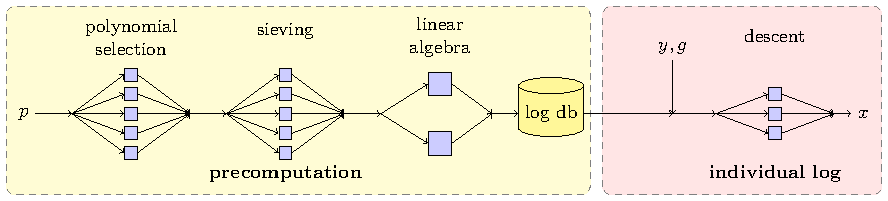
\includegraphics[width=\linewidth]{\LogjamFigures/nfs}

\caption{\textbf{Number field sieve for discrete log}\,---\,%
This algorithm consists of a precomputation stage that depends only on the
prime $p$ and a descent stage that computes individual logarithms. With
sufficient precomputation, an attacker can quickly break any Diffie-Hellman
instances that use a particular $p$.
}
\label{fig:nfs}
\end{figure*}

\paragraph{Risks from common 1024-bit groups}
We explore the implications of precomputation attacks for 768- and 1024-bit
groups, which are widely used in practice and still considered secure. We
estimate the computational resources necessary to compute discrete logs in
groups of these sizes, concluding that 768-bit groups are within range of
academic teams, and 1024-bit groups may plausibly be within range of
nation-state adversaries. In both cases, individual logarithms can be quickly
computed after the initial precomputation.

We then examine evidence from published Snowden documents that suggests NSA
may already be exploiting 1024-bit Diffie-Hellman to decrypt VPN traffic. We
perform measurements to understand the implications of such an attack for
popular protocols, finding that an attacker who could perform precomputations
for ten 1024-bit groups could passively decrypt traffic to about 66\% of IKE
VPNs, 26\% of SSH servers, and 24\% of popular HTTPS sites.

\paragraph{Mitigations and lessons}
In response to the Logjam attack, mainstream browsers have implemented a more
restrictive policy on the size of Diffie-Hellman groups they accept, and
Chrome has discontinued support for finite field key exchanges. We further
recommend that TLS servers disable export-grade cryptography and carefully
vet the Diffie-Hellman groups they use. In the longer term, we advocate that
protocols migrate to elliptic curve Diffie-Hellman.

\section{Diffie-Hellman Cryptanalysis}
\label{sec:dl}

Diffie-Hellman key exchange was the first published public-key
algorithm~\cite{new-directions-in-crypto-1976}. In the simple case of prime
groups, Alice and Bob agree on a prime $p$ and a generator $g$ of a
multiplicative subgroup modulo $p$. Then each generates a random private
exponent, $a$ and $b$. Alice sends $g^a \bmod p$, Bob sends $g^b \bmod p$,
and each computes a shared secret $g^{ab} \bmod p$. While there is also a
Diffie-Hellman exchange over elliptic curve groups, we address only the ``mod
$p$'' case.

The security of Diffie-Hellman is not known to be equivalent to the discrete
logarithm problem, but computing discrete logs remains the best known
cryptanalytic attack. An attacker who can find the discrete log $x$ from $y =
g^x \bmod p$ can easily find the shared secret.

Textbook descriptions of discrete log can be misleading about the
computational tradeoffs, for example by optimizing for computing a
\emph{single} discrete log. In fact, as illustrated in Figure~\ref{fig:nfs},
a single large precomputation on $p$ can be used to efficiently break
\emph{all} Diffie-Hellman exchanges made with that prime.

Diffie-Hellman is typically implemented with prime fields and large group
orders. In this case, the most efficient discrete log algorithm is the number
field sieve
(NFS)~\cite{discrete-log-nfs-1993,virtual-logarithms-2005,nfs-prime-field-2003}.
The algorithm has four stages with different computational properties. The
first three steps are only dependent on the prime $p$ and comprise most of
the computation.

First is \emph{polynomial selection}, in which one finds a polynomial $f(z)$
defining a number field $\QQ[z]/f(z)$ for the computation. This parallelizes
well and is only a small portion of the runtime.

In the second stage, \emph{sieving}, one factors ranges of integers and
number field elements in batches to find many relations of elements, all of
whose prime factors are less than some bound $B$ (called $B$-smooth). Sieving
parallelizes well, but is computationally expensive, because we must search
through and attempt to factor many elements.

In the third stage, \emph{linear algebra}, we construct a large, sparse
matrix consisting of the coefficient vectors of prime factorizations we have
found. This stage can be parallelized in a limited fashion, and produces a
database of logarithms which are used as input to the final stage.

The final stage, \emph{descent}, actually deduces the discrete log of the
target $y$. We re-sieve until we find a set of relations that allow us to
write the logarithm of $y$ in terms of the logarithms in the precomputed
database. Crucially, descent is the only NFS stage that involves $y$ (or
$g$), so polynomial selection, sieving, and linear algebra can be done once
for a prime $p$ and reused to compute the discrete logs of many targets.

The numerous parameters of the algorithm allow some flexibility to reduce
time on some computational steps at the expense of others. For example,
sieving more will result in a smaller matrix, making linear algebra cheaper,
and doing more work in the precomputation makes the final descent step
easier.

\paragraph{Standard primes}
Generating safe primes\footnote{\small An odd prime $p$ is safe when
$(p-1)/2$ is prime.} can be computationally burdensome, so many
implementations use standardized Diffie-Hellman parameters. A prominent
example is the Oakley groups~\cite{rfc2412}, which give ``safe'' primes of
length 768 (Oakley Group 1), 1024 (Oakley Group 2), and 1536 (Oakley Group
5). These groups were published in 1998 and have been used for many
applications since, including IKE, SSH, Tor, and OTR\@.

When primes are of sufficient strength, there seems to be no
disadvantage to reusing them.  However, widespread reuse of
Diffie-Hellman groups can convert attacks that are at the limits of an
adversary's capabilities into devastating breaks, since it allows the
attacker to amortize the cost of discrete log precomputation among
vast numbers of potential targets.

\section{Attacking TLS}
\label{sec:attacking-tls}

TLS supports Diffie-Hellman as one of several possible key exchange
methods, and prior to public disclosure of the attack, about two-thirds of popular HTTPS sites supported it, most
commonly using 1024-bit primes.  However, a smaller number of servers
also support legacy ``export-grade'' Diffie-Hellman using 512-bit
primes that are well within reach of NFS-based
cryptanalysis. Furthermore, for both normal and export-grade
Diffie-Hellman, the vast majority of servers use a handful of common
groups.

In this section, we exploit these facts to construct a novel attack against
TLS\@, which we call the Logjam attack. First, we perform NFS precomputations
for the two most popular 512-bit primes on the web, so that we can quickly
compute the discrete log for any key exchange message that uses one of them.
Next, we show how a man-in-the-middle, so armed, can attack connections
between popular browsers and any server that allows export-grade
Diffie-Hellman, by using a TLS protocol flaw to downgrade the connection to
export-strength and then recovering the session key. We find that this attack
with our precomputations can compromise connections to about 7.8\% of HTTPS
servers among Alexa Top Million domains.

\begin{table}[t]
	\centering\small
	\begin{tabular}{lll}
          \toprule
          Source  & Popularity & Prime \\
          \midrule
          Apache   & 82\% & \tt 9fdb8b8a004544f0045f1737d0ba2e0b\\
                   &      & \tt 274cdf1a9f588218fb435316a16e3741\\
                   &      & \tt 71fd19d8d8f37c39bf863fd60e3e3006\\
                   &      & \tt 80a3030c6e4c3757d08f70e6aa871033\smallskip\\
          mod\_ssl & 10\% & \tt d4bcd52406f69b35994b88de5db89682\\
                   &      & \tt c8157f62d8f33633ee5772f11f05ab22\\
                   &      & \tt d6b5145b9f241e5acc31ff090a4bc711\\
                   &      & \tt 48976f76795094e71e7903529f5a824b\smallskip\\
          (\emph{others\/}) & \ 8\% & (463~distinct primes) \\
          \bottomrule
	\end{tabular}
    \caption{\textbf{Top 512-bit DH primes for TLS}\,---\,%
        8.4\% of Alexa Top~1M HTTPS domains allow \dheexp{}, of which 92.3\% use
        one of the two most popular primes, shown here.
    }
    \label{tab:export-primes}
\end{table}

\subsection{TLS and Diffie-Hellman}

The TLS handshake begins with a negotiation to determine the crypto
algorithms used for the session. The client sends a list of supported
ciphersuites (and a random nonce $cr$) within the \textsf{ClientHello}
message, where each ciphersuite specifies a key exchange algorithm and other
primitives. The server selects a ciphersuite from the client's list and
signals its selection in a \textsf{ServerHello} message (containing a random
nonce $sr$).

TLS specifies ciphersuites supporting multiple varieties of Diffie-Hellman.
Textbook Diffie-Hellman with unrestricted strength is called ``ephemeral''
Diffie-Hellman, or \dhe{}, and is identified by ciphersuites that begin with
\texttt{TLS\_DHE\_*}.\footnote{\small New ciphersuites that use elliptic
curve Diffie-Hellman (\ecdhe{}) are gaining in popularity, but we focus
exclusively on the traditional prime field variety.} In \dhe{}, the server is
responsible for selecting the Diffie-Hellman parameters. It chooses a group
$(p,g)$, computes $g^b$, and sends a \textsf{ServerKeyExchange} message
containing a signature over the tuple $(cr, sr, p, g, g^b)$ using the
long-term signing key from its certificate. The client verifies the signature
and responds with a \textsf{ClientKeyExchange} message containing $g^a$.

To ensure agreement on the negotiation messages, and to prevent downgrade
attacks, each party computes the TLS master secret from $g^{ab}$ and
calculates a MAC of its view of the handshake transcript. These MACs are
exchanged in a pair of \textsf{Finished} messages and verified by the
recipients.

\paragraph{Export-grade Diffie-Hellman}
To comply with 1990s-era U.S. export restrictions on cryptography, SSL 3.0
and TLS 1.0 supported reduced-strength \dheexp{} ciphersuites that were
restricted to primes no longer than 512 bits. In all other respects,
\dheexp{} protocol messages are identical to \dhe{}. The relevant export
restrictions are no longer in effect, but many servers maintain support for
backwards compatibility.

To understand how HTTPS servers in the wild use Diffie-Hellman, we modified
the ZMap~\cite{zmap-2013} toolchain to offer \dhe{} and \dheexp{}
ciphersuites and scanned TCP/443 on both the full public IPv4 address space
and the Alexa Top~1M domains. The scans took place in March 2015. Of 539,000
HTTPS sites among Top~1M domains, we found that 68.3\% supported \dhe{} and
8.4\% supported \dheexp{}. Of 14.3~million IPv4 HTTPS servers with
browser-trusted certificates, 23.9\% supported \dhe{} and 4.9\% \dheexp{}.

\iffalse
\begin{table}[t]
	\centering\small
	\begin{tabular}{rllrl}
    \toprule
	Fraction & Source & Year & Bits & Prime \\
    \midrule
0.8255 & Apache 2.2 & 2005 & 512 & \texttt{9fdb8b8a}$\ldots$\texttt{aa871033} \\
0.0997 & mod\_ssl & 1999 & 512 & \texttt{d4bcd524}$\ldots$\texttt{9f5a824b}\\
0.0414 & IKE & 2000 & 2048 & \texttt{fff}$\ldots$\texttt{c90fdaa2}$\ldots$\texttt{fff} \\
0.0069 & JDK & 2003 & 512 & \texttt{fca682ce}$\ldots$\texttt{37592e17} \\
0.0012 & (unknown)& --- & 512 & \texttt{acc8149e}$\ldots$\texttt{67ec1505} \\
\midrule
0.0253 & \multicolumn{4}{c}{\emph{other primes}} \\
    \bottomrule
	\end{tabular}
    \label{tab:export-primes}
\end{table}
\fi

While the TLS protocol allows servers to generate their own Diffie-Hellman
parameters, just two 512-bit primes account for 92.3\% of Alexa Top~1M
domains that support \dheexp{} (Table~\ref{tab:export-primes}), and 92.5\% of
all servers with browser-trusted certificates that support \dheexp{}. The
most popular 512-bit prime was hard-coded into many versions of Apache; the
second most popular is the \texttt{mod\_ssl} default for \dheexp{}.

\subsection{Active Downgrade to Export-Grade DHE}
\label{sec:dhead}

\begin{figure}[t]
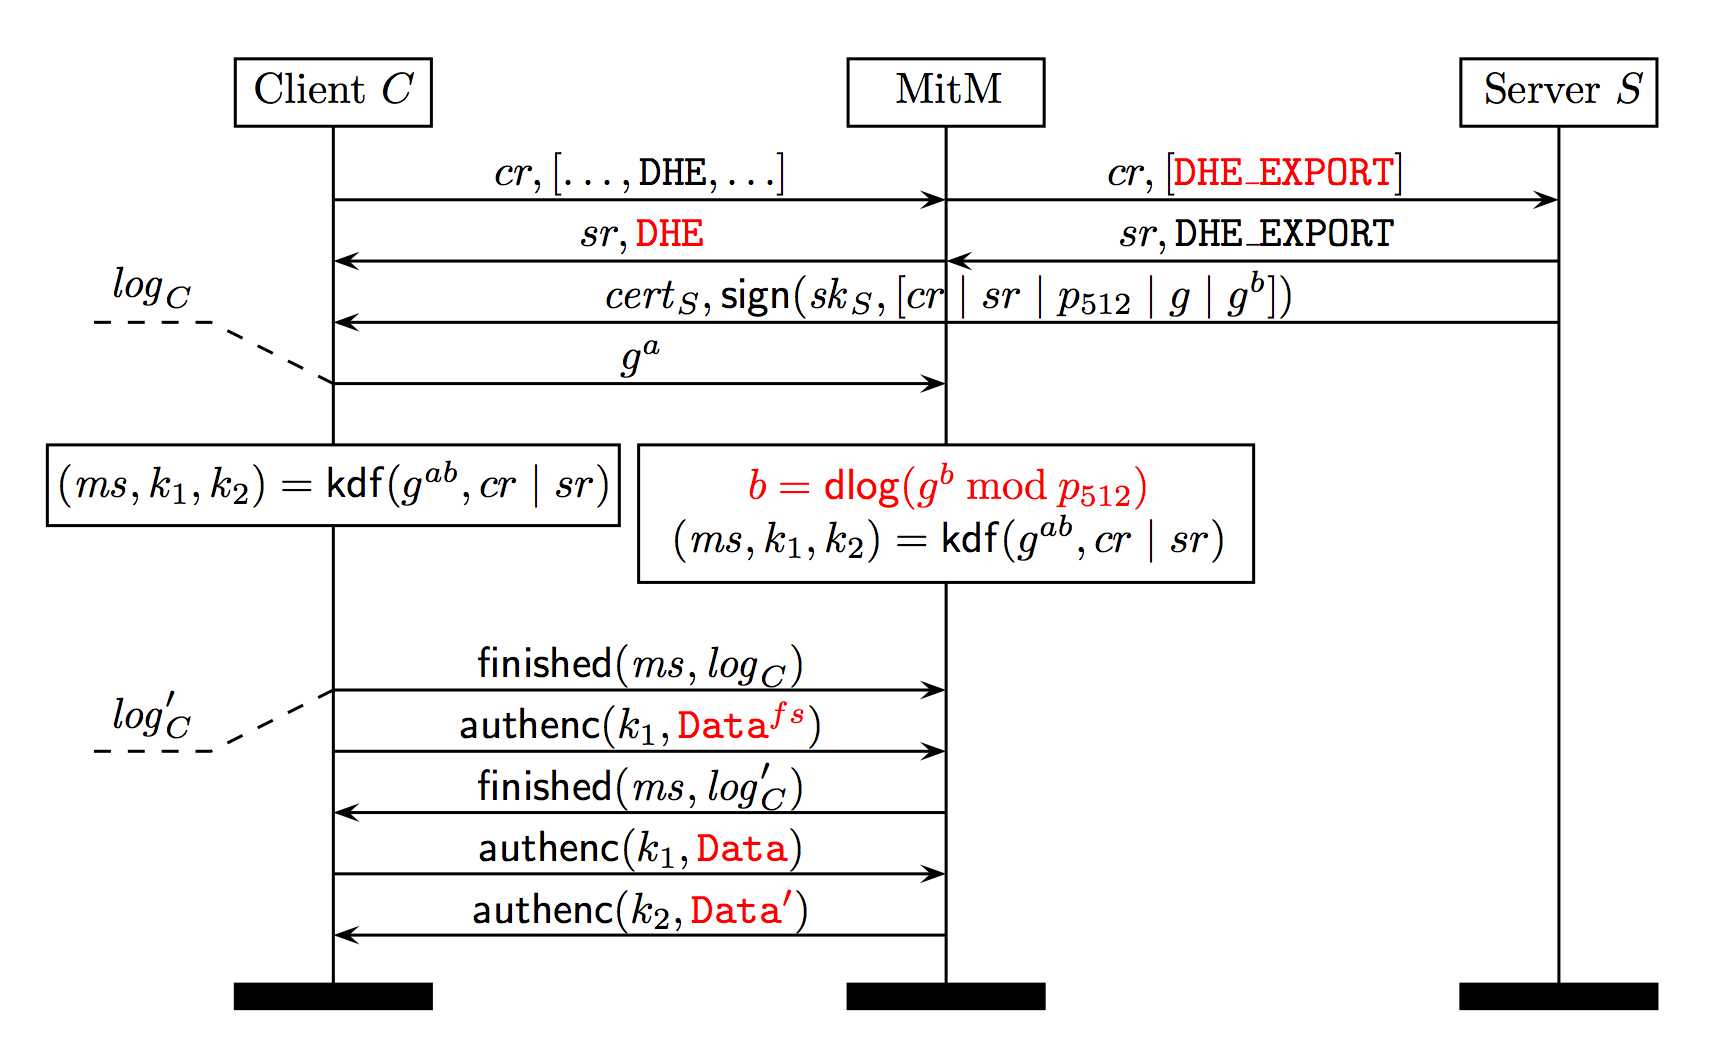
\includegraphics[width=\linewidth]{\LogjamFigures/mitm-dhe-export}
    \caption{\textbf{The Logjam attack}\,---\,%
    A man-in-the-middle can force TLS clients to use export-strength DH with
    any server that allows \dheexp{}. Then, by finding the 512-bit discrete
    log, the attacker can learn the session key and arbitrarily read or
    modify the contents. $\AData^{fs}$ refers to False Start application data
    that some TLS clients send before receiving the server's
    \textsf{Finished} message.}
    \label{fig:mitm-export}
\end{figure}

Given the widespread use of these primes, an attacker with the ability to
compute discrete logs in 512-bit groups could efficiently break \dheexp{}
handshakes for about 8\% of Alexa Top~1M HTTPS sites, but modern browsers
never negotiate export-grade ciphersuites. To circumvent this, we show how an
attacker can downgrade a regular \dhe{} connection to use a \dheexp{} group,
and thereby break both the confidentiality and integrity of application data.

The attack, which we call Logjam, is depicted in Figure~\ref{fig:mitm-export}
and relies on a flaw in the way TLS composes \dhe{} and \dheexp{}. When a
server selects \dheexp{} for a handshake, it proceeds by issuing a signed
\textsf{ServerKeyExchange} message containing a 512-bit $p_{512}$, but the
structure of this message is identical to the message sent during standard
\dhe{} ciphersuites. Critically, the signed portion of the server's message
fails to include any indication of the specific ciphersuite that the server
has chosen. Provided that a client offers \dhe{}, an active attacker can
rewrite the client's \textsf{ClientHello} to offer a corresponding \dheexp{}
ciphersuite accepted by the server and remove other ciphersuites that could
be chosen instead. The attacker rewrites the \textsf{ServerHello} response to
replace the chosen \dheexp{} ciphersuite with a matching non-export
ciphersuite and forwards the \textsf{ServerKeyExchange} message to the client
as is. The client will interpret the export-grade tuple $(p_{512}, g, g^b)$
as valid \dhe{} parameters chosen by the server and proceed with the
handshake. The client and server have different handshake transcripts at this
stage, but an attacker who can compute $b$ in close to real time can then
derive the master secret and connection keys to complete the handshake with
the client.

There are two remaining challenges in implementing this active downgrade
attack. The first is to compute individual discrete logs in close to real
time, and the second is to delay handshake completion until the discrete log
computation has had time to finish.

\subsection{512-bit Discrete Log Computations}
\label{subsec:512bit-dl-computation}

We modified CADO-NFS~\cite{cado-nfs-2.3} to implement the number field sieve
discrete log algorithm and applied it to the top two \dheexp{} primes shown
in Table~\ref{tab:export-primes}. Precomputation took 7~days for each prime,
after which computing individual logarithms requires a median of 70~seconds.

\paragraph{Precomputation}
As illustrated in Figure~\ref{fig:nfs}, the precomputation phase includes the
polynomial selection, sieving, and linear algebra steps. For this
precomputation, we deliberately sieved more than strictly necessary. This
enabled two optimizations: first, with more relations obtained from sieving,
we eventually obtain a larger database of known logarithms, which makes the
descent faster. Second, more sieving relations also yield a smaller linear
algebra step, which is desirable because sieving is much easier to
parallelize than linear algebra.
%\looseness=-1

For the polynomial selection and sieving steps, we used idle time on
2000--3000 CPU cores in parallel. Polynomial selection ran for about 3~hours
(7,600 core-hours). Sieving ran for 15~hours (21,400 core-hours). This
sufficed to collect 40\,M relations of which 28\,M were unique, involving
15\,M primes of at most 27~bits.

From this data set, we obtained a square matrix with 2.2\,M rows and columns,
with 113 nonzero coefficients per row on average. We solved the corresponding
linear system on a 36-node cluster using the block Wiedemann
algorithm~\cite{coppersmith-block-wiedemann-1994,thome-block-wiedemann-2002}.
Using unoptimized code, the computation finished in 120 hours (60,000
core-hours).

The experiment above was done with CADO-NFS in early 2015. As of 2017,
release 2.3 of CADO-NFS~\cite{cado-nfs-2.3} performs 20\% faster for sieving,
and drastically faster for linear algebra, since 9,000 core-hours suffice to
solve the same linear system on the same hardware. In total, the wall-clock
time for each precomputation was slightly over one week in 2015, and is
reduced to about two days with current hardware and more recent software.

\paragraph{Descent}
Once this precomputation was finished, we were able to run the final descent
step to compute individual discrete logs in about a minute. We implemented
the descent calculation in a mix of Python and C\@. On average, computing
individual logarithms took about 70~seconds, but the time varied from 34 to
206 seconds on a server with two 18-core Intel Xeon E5-2699 CPUs. For
purposes of comparison, a single 512-bit RSA factorization using the CADO-NFS
implementation takes about 4 days of wall-clock time on the computer used for
the descent\cite{cado-nfs-2.3}.

% reference: revision 580f1f1 of CADO-NFS with tasks.sieve.qmin=15470309
% on a catrel node:
% Total cpu/elapsed time for entire factorization: 1.06608e+07/351570
% 351570/3600/24 = 4.07

\subsection{Active Attack Implementation}
The main challenge in performing this attack is to compute the shared secret
$g^{ab}$ before the handshake completes in order to forge a \textsf{Finished}
message from the server. With our descent implementation, the computation
takes an average of 70 seconds, but there are several ways an attacker can
work around this delay:

\paragraph{Non-browser clients}
Different TLS clients impose different time limits, after which they kill the
connection. Command-line clients such as \texttt{curl} and \texttt{git} have
long or no timeouts, and we can hijack their connections without difficulty.

\paragraph{TLS warning alerts}
Web browsers tend to have shorter timeouts, but we can keep their connections
alive by sending TLS warning alerts, which are ignored by the browser but
reset the handshake timer. For example, this allows us to keep Firefox TLS
connections alive indefinitely.

\paragraph{Ephemeral key caching}
Many TLS servers do not use a fresh value $b$ for each connection, but
instead compute $g^b$ once and reuse it for multiple negotiations. For
example, F5 BIG-IP load balancers will reuse $g^b$ by default. Microsoft
Schannel caches $g^b$ for two hours---this setting is hard-coded. For these
servers, an attacker can compute the discrete log of $g^b$ from one
connection and use it to attack later handshakes.

\paragraph{TLS False Start}
Even when clients enforce shorter timeouts and servers do not reuse values
for $b$, the attacker can still break the confidentiality of user requests
that use TLS False Start. Recent versions of Chrome, Internet Explorer, and
Firefox implement False Start, but their policies on when to enable it vary.
Firefox 35, Chrome 41, and Internet Explorer (Windows 10) send False Start
data with \dhe{}\@. In these cases, a man-in-the-middle can record the
handshake and decrypt the False Start payload at leisure.

\section{Nation-State Threats to DH}
\label{sec:nationstate}

The previous sections demonstrate the existence of practical attacks against
Diffie-Hellman key exchange as currently used by TLS\@. However, these
attacks rely on the ability to downgrade connections to export-grade crypto.
In this section we address the following question: how secure is
Diffie-Hellman in broader practice, as used in other protocols that do not
suffer from downgrade, and when applied with stronger groups?

\begin{table*}
\centering\small
\begin{tabular}{rrrrrrl@{}}
\toprule
  & \multicolumn{2}{c}{Sieving} & \multicolumn{2}{c}{Linear Algebra} & \multicolumn{1}{c}{Descent} \\
 \cmidrule(r){2-3} \cmidrule(r){4-5} \cmidrule(){6-6}
 & $\log_2B$ & core-years  & rows & core-years  & core-time   \\
\midrule
% timings below from CADO-NFS revision 580f1f1 on a catrel node
% with tasks.sieve.qmin=15470309
% Info:Lattice Sieving: Total CPU time: 9.53745e+06s -> 0.30 cpu year
% Info:Filtering - Merging: Merged matrix has 4146413 rows and total weight 704890615 (170.0 entries per row on average)
% Info:Linear Algebra: Krylov: WCT time 21706.76
% Info:Linear Algebra: Lingen CPU time 4834.58, WCT time 218.43
% Info:Linear Algebra: Mksol: WCT time 11599.56
% Linear Algebra: total WCT = 33524.75
% thus cpu <= 32*WCT <= 1.072792e6 (32 threads) <= 0.03 cpu year
\multicolumn{1}{r}{RSA-512} &
29 & 0.3 &  4.2M & 0.03 &  
& \scriptsize\quad Timings with default CADO-NFS parameters.\\
\multicolumn{1}{r}{DH-512} &
27& 2.5 &  2.2M & 1.1 &  10\,mins
& \scriptsize\quad For the computations in this paper; may be suboptimal.\\
\cmidrule{1-7}
\multicolumn{1}{r}{RSA-768} & 
37& 800 & 250M & 100 &
& \scriptsize\quad Est.\ based on~\cite{rsa768} with less sieving.  \\
%\multicolumn{1}{r}{DH-768} &
%  35 & 8,000 & 150M & 28,500 & 2\,days
%& \scriptsize\quad Est.\ based on~\cite{rsa768,dlp180} and our own experiments. \\
\multicolumn{1}{r}{DH-768} &
36 & 4,000 & 24M & 920 & 43\,hours
    & \scriptsize\quad Data from~\cite[Table 1]{Kleinjung2017}.\\
\cmidrule{1-7}
\multicolumn{1}{r}{RSA-1024} &
42& $\approx$1,000,000  & $\approx$8.7B & $\approx$120,000 & 
& \scriptsize\quad Crude estimate based on complexity formula. \\
%\multicolumn{1}{r}{DH-1024} &
%   40 & 10,000,000 & 5.2B & 35,000,000 & 30\,days
%& \scriptsize\quad Est.\ based on complexity formula and our experiments. \\
\multicolumn{1}{r}{DH-1024} &
   40 & $\approx$5,000,000 & $\approx$0.8B & $\approx$1,100,000 & 30\,days
& \scriptsize\quad Crude estimate based on formula and our experiments. \\
\bottomrule
\end{tabular}

\caption{\textbf{Estimating costs for factoring and discrete log}.
For sieving, we give one important parameter, which is the number of bits of the
smoothness bound
{\tt B}.
For linear algebra, all costs for DH are for
safe primes; for DSA primes with $q$ of 160 bits, this should be
divided by 6.4 for 1024 bits, 4.8 for 768 bits, and 3.2 for 512 bits.}

\label{tab:costs}
\end{table*}



To answer this question we must first examine how the number field sieve for
discrete log scales to 768- and 1024-bit groups. As we argue below, 768-bit
groups in relatively widespread use are now within reach for academic
computational resources. Additionally, performing precomputations for a small
number of 1024-bit groups is plausibly within the resources of nation-state
adversaries. The precomputation would likely require special-purpose
hardware, but would not require any major algorithmic improvements. In light
of these results, we examine several standard Internet security
protocols---IKE, SSH, and TLS---to determine their vulnerability. Although
the cost of the precomputation for a 1024-bit group is several times higher
than for an RSA key of equal size, a one-time investment could be used to
attack millions of hosts, due to widespread reuse of the most common
Diffie-Hellman parameters. Finally, we apply this new understanding to a set
of recently published documents to evaluate the hypothesis that the National
Security Agency has {\em already} implemented such a capability.

\subsection{Scaling NFS to 768- and 1024-bit DH}

Estimating the cost for discrete log cryptanalysis at larger key sizes is far
from straightforward due to the complexity of parameter tuning. We attempt
estimates up to 1024-bit discrete log based on the existing literature and
our own experiments but further work is needed for greater confidence. We
summarize all the costs, measured or estimated, in Table~\ref{tab:costs}.

\paragraph{DH-768: Completed in 2016}
At the time of disclosure, the latest discrete log record was a 596-bit
computation. Based on that work, and on prior experience with the 768-bit
factorization record in 2009~\cite{factor-rsa-768}, we made the conservative
prediction that it was possible, as explained in~\S\ref{sec:dl}, to put more
computational effort into sieving for the discrete log case than for
factoring, so that the linear algebra step would run on a slightly smaller
matrix. This led to a runtime estimate of around 35,000 core-years, most of
which was spent on linear algebra.

This estimate turned out be overly conservative, for several reasons. First,
there have been significant improvements in our software implementation
(see~\S\ref{subsec:512bit-dl-computation}). In addition, our estimate did not
use the Joux-Lercier alternative polynomial selection
method~\cite[\S2.1]{nfs-prime-field-2003}, which is specific to discrete
logs. For 768-bit discrete logs, this polynomial selection method leads to a
significantly smaller computational cost.

In 2016, Kleinjung et al.\ completed a 768-bit discrete log
computation~\cite{compute-dlog-768}. While this is a massive computation on
the academic scale, a computation of this size has likely been within reach
of nation-states for more than a decade. This data is mentioned in
Table~\ref{tab:costs}.

\paragraph{DH-1024: Plausible with nation-state resources}
Experimentally extrapolating sieving parameters to the 1024-bit case is
difficult due to the tradeoffs between the steps of the algorithm and their
relative parallelism. The prior work proposing parameters for factoring a
1024-bit RSA key is thin and we resort to extrapolating from asymptotic
complexity. For the number field sieve, the complexity is
$\exp\big((k+o(1))(\log N)^{1/3}(\log\log N)^{2/3}\big),$ where $N$ is the
integer to factor or the prime modulus for discrete log and $k$ is an
algorithm-specific constant. This formula is inherently imprecise, since the
$o(1)$ in the exponent can hide polynomial factors. This complexity formula,
with $k=1.923$, describes the overall time for both discrete log and
factorization, which are both dominated by sieving and linear algebra in the
precomputation. Evaluating the formula for 768- and 1024-bit $N$ gives us
estimated multiplicative factors by which time and space will increase from
the 768- to the 1024-bit case.

For 1024-bit precomputation, the total time complexity can be expected to
increase by a factor of 1220 using the complexity formula, while space
complexity increases by its square root, approximately 35. These ratios are
relevant for both factorization and discrete log since they have the same
asymptotic behavior. For DH-1024, we get a total cost estimate for the
precomputation of about 6M core-years.

The time complexity for each individual log after the precomputation should
be multiplied by $L_{2^{1024}}(1.206)/L_{2^{768}}(1.206)\approx86$, where
$k=1.206$ follows from~\cite{hidden-snfs-1024-2017}. This last number does
not correspond to what we observed in practice and we attribute that to the
fact that the descent step has been far less studied.

In practice, it is not uncommon for estimates based merely on the complexity
formula to be off by a factor of 10. Estimates of Table~\ref{tab:costs} must
therefore be considered with due caution.

For 1024-bit descent, we experimented with our early-abort implementation to
inform our estimates for descent initialization, which should dominate the
individual discrete log computation. For a random target in Oakley Group~2,
initialization took 22 core-days, and yielded a few primes of at most 130
bits to be descended further. In twice this time, we reached primes of about
110 bits. At this point, we were certain to have bootstrapped the descent and
could continue down to the smoothness bound in a few more core-days if proper
sieving software were available. Thus we estimate that a 1024-bit descent
would take about 30~core-days, once again easily parallelizable.

\paragraph{Costs in hardware}
Although several millions of core-years is a massive computational effort, it
is not necessarily out of reach for a nation-state. At this scale,
significant cost savings could be realized by developing application-specific
hardware given that sieving is a natural target for hardware implementation.
To our knowledge, the best prior description of an ASIC implementation of
1024-bit sieving is the 2007 work of Geiselmann and
Steinwandt~\cite{hardware-scaling-nfs-2007}. Updating their estimates for
modern techniques and adjusting parameters for discrete log allows us to
extrapolate the financial and time costs.

We increase their chip count by a factor of ten to sieve more and save on
linear algebra as above giving an estimate of 3M chips to complete sieving in
one year. Shrinking the dies from the 130~nm technology node used in the
paper to a more modern size reduces costs as transistors are cheaper at newer
technologies. With standard transistor costs and utilization, it would cost
about \$2 per chip to manufacture after fixed design and tape-out costs of
roughly \$2M~\cite{jefferies-report-2012}. This suggests that an \$8M
investment would buy enough ASICs to complete the DH-1024 sieving
precomputation in one year. Since a step of descent uses sieving, the same
hardware could likely be reused to speed calculations of individual
logarithms.

Estimating the financial cost for the linear algebra is more difficult since
there has been little work on designing chips that are suitable for the
larger fields involved in discrete log. To derive a rough estimate, we can
begin with general purpose hardware and the core-year estimate from
Table~\ref{tab:costs}. Using the 300,000 CPU core Titan supercomputer it
would take 4~years to complete the 1024-bit linear algebra stage
(notwithstanding the fact that estimates from Table~\ref{tab:costs} are known
to be extremely coarse, and could be optimistic by a factor of maybe 10).
Titan was constructed in 2012 for \$94M, suggesting a cost of \$0.5B in
supercomputers to finish this step in a year. In the context of
factorization, moving linear algebra from general purpose CPUs to ASICs has
been estimated to reduce costs by a factor of
80~\cite{improving-linear-algebra-nfs-2005}. If we optimistically assume that
a similar reduction can be achieved for discrete log, the hardware cost to
perform the linear algebra for DH-1024 in one year is plausibly on the order
of tens of millions of dollars.

To put this dollar figure in context, the FY\,2012 budget for the U.S.
Consolidated Cryptologic Program (which includes the NSA) was \$10.5
billion\footnote{\small The National Science Foundation's budget was \$7
billion.}~\cite{black-budget-leak-2013}. The 2013 budget request, which
prioritized investment in ``groundbreaking cryptanalytic capabilities to
defeat adversarial cryptography and exploit internet traffic'' included
notable \$100M+ increases in two programs under Cryptanalysis \& Exploitation
Services: ``Cryptanalytic IT Systems'' (to \$247M), and the cryptically named
``PEO Program C'' (to \$360M)~\cite{black-budget-leak-2013}.

\subsection{Is NSA Breaking 1024-bit DH?}

Our calculations suggest that it is plausibly within NSA's resources to have
performed number field sieve precomputations for a small number of 1024-bit
Diffie-Hellman groups. This would allow them to break any key exchanges made
with those groups in close to real time. If true, this would answer one of
the major cryptographic questions raised by the Edward Snowden leaks: How is
NSA defeating the encryption for widely used VPN protocols?

Virtual private networks (VPNs) are widely used for tunneling business or
personal traffic across potentially hostile networks. We focus on the
Internet Protocol Security (IPsec) VPN protocol using the Internet Key
Exchange (IKE) protocol for key establishment and parameter negotiation and
the Encapsulating Security Payload (ESP) protocol for protecting packet
contents.

\paragraph{IKE}
There are two versions, IKEv1 and IKEv2, which differ in message structure
but are conceptually similar. For the sake of brevity, we will use IKEv1
terminology~\cite{rfc7296}.

\newcommand{\skeyid}{\textsf{\small SKEYID}}
\newcommand{\keymat}{\textsf{\small KEYMAT}}
\newcommand{\psk}{\textsf{\small PSK}}

Each IKE session begins with a Phase~1 handshake in which the client and
server select a Diffie-Hellman group from a small set of standardized
parameters and perform a key exchange to establish a shared secret. The
shared secret is combined with other cleartext values transmitted by each
side, such as nonces and cookies, to derive a value called \skeyid\@. When
authenticated with a pre-shared key (PSK) in IKEv1, the PSK value is
incorporated into the derivation of \skeyid.

The resulting \skeyid\ is used to encrypt and authenticate a Phase~2
handshake. Phase~2 establishes the parameters and key material, \keymat, for
protecting the subsequently tunneled traffic. Ultimately, \keymat{} is
derived from \skeyid, additional nonces, and the result of an optional
Phase~2 Diffie-Hellman exchange.

\paragraph{NSA's VPN exploitation process}
Documents published by Der Spiegel describe NSA's ability to decrypt VPN
traffic using passive eavesdropping and without message injection or
man-in-the-middle attacks on IPsec or IKE\@. Figure~\ref{fig:scarynsafigure}
illustrates the flow of information required to decrypt the tunneled traffic.

\begin{figure}
    \noindent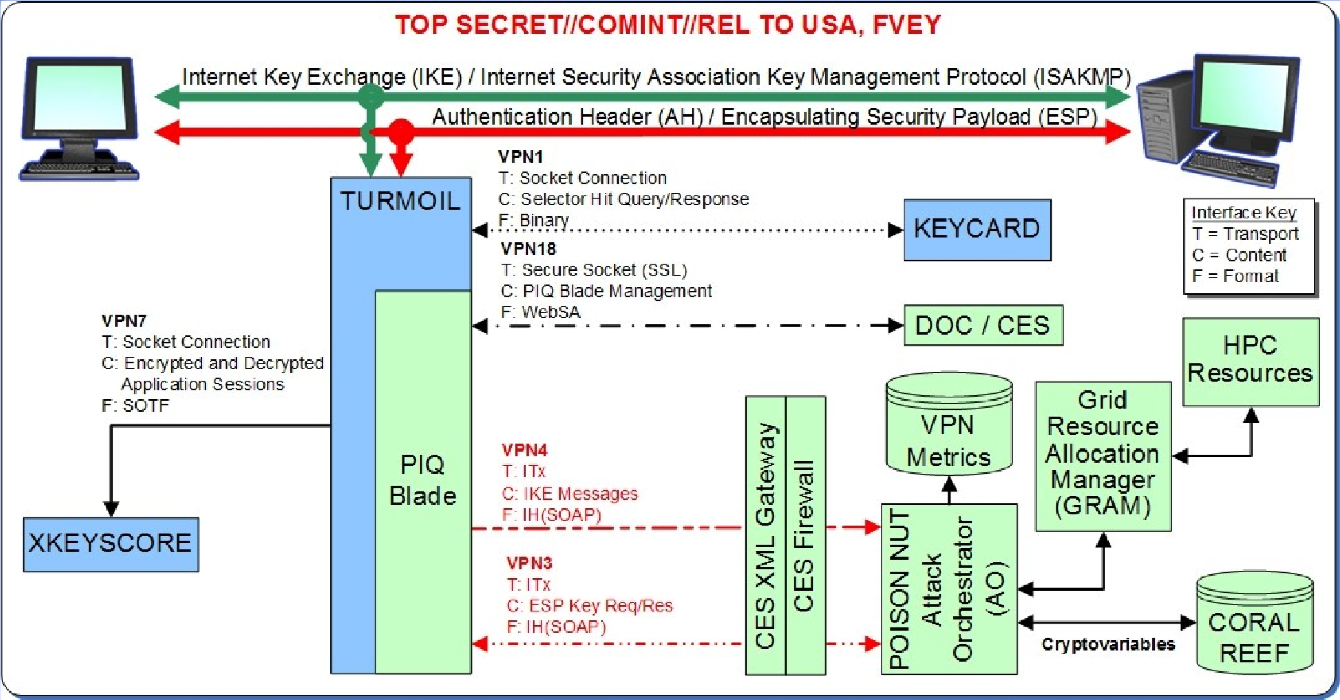
\includegraphics[width=\linewidth]{\LogjamFigures/NSA_combined.png}
    \caption{\textbf{NSA's VPN decryption infrastructure}\,---\,%
    This classified illustration published by Der
    Spiegel~\cite{media-35526} shows captured IKE handshake messages
    being passed to a high-performance computing system, which returns the
    symmetric keys for ESP session traffic. The details of this attack are
    consistent with an efficient break for 1024-bit Diffie-Hellman.}
    \label{fig:scarynsafigure}
\end{figure}

\begin{table*}[t]
\small
\centering
\begin{tabular}{lrrrr}
\toprule
              & \multicolumn{4}{c}{\emph{Vulnerable servers, if the attacker can precompute for \ldots}} \\
\cmidrule{2-5}
%\multicolumn{1}{r}{\emph{If the attacker can precompute \ldots.}}
              & all 512-bit groups & all 768-bit groups & one 1024-bit group & ten 1024-bit groups\\  
\midrule
HTTPS Top~1M w/ active downgrade\qquad\strut & 45,100 (8.4\%) & 45,100 (8.4\%) & 205,000 (37.1\%) & 309,000 (56.1\%) \\
HTTPS Top~1M & 118 (0.0\%) & 407 (0.1\%) & 98,500 (17.9\%) & 132,000 (24.0\%) \\
HTTPS Trusted w/ active downgrade & 489,000 (3.4\%) & 556,000 (3.9\%) & 1,840,000 (12.8\%) & 3,410,000 (23.8\%) \\ 
HTTPS Trusted &  1,000 (0.0\%) & 46,700 (0.3\%) & 939,000 (6.56\%) & 1,430,000 (10.0\%)\medskip\\
IKEv1 IPv4  & -- & 64,700 (2.6\%) & 1,690,000 (66.1\%)& 1,690,000 (66.1\%) \\
IKEv2 IPv4  & -- & 66,000 (5.8\%) & 726,000 (63.9\%) & 726,000 (63.9\%)\medskip \\
SSH   IPv4  & -- & -- & 3,600,000 (25.7\%) & 3,600,000 (25.7\%) \\
\bottomrule

\end{tabular}
\caption{\textbf{Estimated impact of Diffie-Hellman attacks in early 2015.}
We used Internet-wide scanning to estimate the number of real-world servers for which 
typical connections could be compromised by attackers with various levels of computational
resources. For HTTPS, we provide figures with and without downgrade attacks on the chosen ciphersuite. All others are passive attacks.
}
\end{table*}


When the IKE/ESP messages of a VPN of interest are collected, the IKE
messages and a small amount of ESP traffic are sent to the Cryptanalysis and
Exploitation Services (CES)~\cite{media-35526,media-35529,media-35515}.
Within the CES enclave, a specialized ``attack orchestrator'' attempts to
recover the ESP decryption key with assistance from high-performance
computing resources as well as a database of known PSKs
(``CORALREEF'')~\cite{media-35529,media-35526,media-35515}. If the recovery
was successful, the decryption key is returned from CES and used to decrypt
the buffered ESP traffic such that the encapsulated content can be
processed~\cite{media-35529,media-35522}.

\paragraph{Evidence for a discrete log attack}
The ability to decrypt VPN traffic does not necessarily indicate a defeat of
Diffie-Hellman. There are, however, several features of the described
exploitation process that support this hypothesis.

The IKE protocol has been extensively
analyzed~\cite{ike-security-2002,ike-nrl-1999} and is not believed to be
exploitable in standard configurations under passive eavesdropping attacks.
Absent a vulnerability in the key derivation function or transport
encryption, the attacker must recover the decryption keys. This requires the
attacker to calculate \skeyid{} generated from the Phase~1 Diffie-Hellman
shared secret after passively observing an IKE handshake.

While IKE is designed to support a range of Diffie-Hellman groups, our
Internet-wide scans (\S\ref{sec:1024effects}) show that the vast majority of
IKE endpoints select one particular 1024-bit DH group even when offered
stronger groups. Conducting an expensive, but feasible, precomputation for
this single 1024-bit group (Oakley Group 2) would allow the efficient
recovery of a large number of Diffie-Hellman shared secrets used to derive
\skeyid{} and the subsequent \keymat.

Given an efficient oracle for solving the discrete logarithm problem, attacks
on IKE are possible provided that the attacker can obtain the following:
$(1)$ a complete two-sided IKE transcript, and $(2)$ any PSK used for
deriving {\skeyid} in IKEv1. The available documents describe both of these
as explicit prerequisites for the VPN exploitation process outlined above and
provide the reader with internal resources available to meet these
prerequisites~\cite{media-35515}.

Of course, this explanation is not dispositive and the possibility remains
that NSA could defeat VPN encryption using alternative means. A published NSA
document refers to the use of a router ``implant'' to allow decryption of
IPsec traffic indicating that the use of targeted malware is possible. This
implant ``allows passive exploitation with just ESP''~\cite{media-35515}
without the prerequisite of collecting the IKE handshake messages. This
indicates that it is an alternative mechanism to the attack described above.

The most compelling argument for a pure cryptographic attack is the
generality of the NSA's VPN exploitation process. This process appears to be
applicable across a broad swath of VPNs without regard to endpoint's identity
or the ability to compromise individual endpoints.


\subsection{Effects of a 1024-bit Break}
\label{sec:1024effects}

In this section, we use Internet-wide scanning to assess the impact of a
hypothetical DH-1024 break on IKE, SSH, and HTTPS\@. Our measurements,
performed in early 2015, indicate that these protocols would be subject to
widespread compromise by a nation-state attacker who had the resources to
invest in precomputation for a small number of 1024-bit groups.

\paragraph{IKE}
We measured how IPsec VPNs use Diffie-Hellman in practice by scanning a 1\%
random sample of the public IPv4 address space for IKEv1 and IKEv2 (the
protocols used to initiate an IPsec VPN connection) in May~2015. We used the
ZMap UDP probe module to measure support for Oakley Groups~1 and~2 (two
popular 768- and 1024-bit, built-in groups) and which group servers prefer.
Of the 80K hosts that responded with a valid IKE packet, 44.2\% were willing
to negotiate a connection using one of the two groups. We found that 31.8\%
of IKEv1 and 19.7\% of IKEv2 servers support Oakley Group~1 (768-bit) while
86.1\% and 91.0\% respectively supported Oakley Group~2 (1024-bit). In our
sample of IKEv1 servers, 2.6\% of profiled servers preferred the 768-bit
Oakley Group~1 and 66.1\% preferred the 1024-bit Oakley Group~2. For IKEv2,
5.8\% of profiled servers chose Oakley Group~1, and 63.9\% chose Oakley
Group~2.

\paragraph{SSH}
All SSH handshakes complete either a finite field or elliptic curve
Diffie-Hellman exchange. The protocol explicitly defines support for Oakley
Group~2 (1024-bit) and Oakley Group~14 (2048-bit) but also allows a
server-defined group to be negotiated. We scanned 1\% random samples of the
public IPv4 address space in April 2015. We find that 98.9\% of SSH servers
support the 1024-bit Oakley Group~2, 77.6\% support the 2048-bit Oakley
Group~14, and 68.7\% support a server-defined group\@.

During the SSH handshake, the server selects the client's highest priority
mutually supported key exchange algorithm. To estimate what servers will
prefer in practice, we performed a scan in which we mimicked the algorithms
offered by OpenSSH 6.6.1p1, the latest version of OpenSSH\@. In this scan,
21.8\% of servers preferred the 1024-bit Oakley Group~2, and 37.4\% preferred
a server-defined group. 10\% of the server-defined groups were 1024-bit, but,
of those, nearly all provided Oakley Group~2 rather than a custom group.

Combining these equivalent choices, we find that a nation-state adversary who
performed NFS precomputations for the 1024-bit Oakley Group~2 could passively
eavesdrop on connections to 3.6M (25.7\%) publicly accessible SSH servers.

\paragraph{HTTPS}
\dhe is commonly deployed on web servers. 68.3\% of Alexa Top~1M sites
support \dhe, as do 23.9\% of sites with browser-trusted certificates. Of the
Top~1M sites that support \dhe, 84\% use a 1024-bit or smaller group, with
94\% of these using one of five groups.

Despite widespread support for \dhe, a passive eavesdropper can only decrypt
connections that organically agree to use Diffie-Hellman. We estimate the
number of sites for which this will occur by offering the same sets of
ciphersuites as Chrome, Firefox, and Safari. Approximately 24.0\% of browser
connections with HTTPS-enabled Top~1M sites (and 10\% with browser-trusted
sites) will negotiate \dhe with one of the ten most popular 1024-bit primes;
17.9\% of connections with Top~1M sites could be passively eavesdropped given
the precomputation for a single 1024-bit prime.


\section{Recommendations}
\label{sec:lessons}

In this section, we present concrete recommendations to recover the expected
security of Diffie-Hellman.

\paragraph{Transition to elliptic curves.}
Transitioning to elliptic curve Diffie-Hellman (ECDH) key exchange avoids all
known feasible cryptanalytic attacks. Current elliptic curve discrete log
algorithms do not gain as much of an advantage from precomputation. In
addition, ECDH keys are shorter and computations are faster. We recommend
transitioning to elliptic curves; this is the most effective solution to the
vulnerabilities in this paper. We note that in August 2015, the NSA announced
that it was planning to transition away from elliptic curve cryptography for
its Suite B cryptographic algorithms and would replace them with algorithms
resistant to quantum computers~\cite{nsa-suiteb}. However, since no fully
vetted and standardized quantum-resistant algorithms exist currently,
elliptic curves remain the most secure choice for public key operations.

\paragraph{Increase minimum key strengths.}
To protect against the Logjam attack, server operators should disable \dheexp
and configure \dhe ciphersuites to use primes of 2048 bits or larger.
Browsers and clients should raise the minimum accepted size for
Diffie-Hellman groups to at least 1024 bits in order to avoid downgrade
attacks.

\paragraph{Don't deliberately weaken crypto.}
The Logjam attack illustrates the fragility of cryptographic ``front doors''.
Although the key sizes originally used in \dheexp were intended to be
tractable only to NSA, two decades of algorithmic and computational
improvements have significantly lowered the bar to attacks on such key sizes.
Despite the eventual relaxation of crypto export restrictions and subsequent
attempts to remove support for \dheexp{}, the technical debt induced by the
additional complexity has left implementations vulnerable for decades. Like
FREAK~\cite{freak-attack-2015}, our attacks warn of the long-term
debilitating effects of deliberately weakening cryptography.


\section{Conclusion}
\label{sec:conclusion}

We find that Diffie-Hellman key exchange, as used in practice, is often less
secure than widely believed. The problems stem from the fact that the number
field sieve for discrete log allows an attacker to perform a single
precomputation that depends only on the group, after which computing
individual logarithms in that group has a far lower cost. Although this is
well known to cryptographers, it apparently has not been widely understood by
system builders. Likewise, many cryptographers did not appreciate that a
large fraction of Internet communication depends on a few small, widely
shared groups.
%\looseness=-1

A key lesson is that cryptographers and creators of practical systems need to
work together more effectively. System builders should take responsibility
for being aware of applicable cryptanalytic attacks. Cryptographers should
involve themselves in how crypto is actually being applied, such as through
engagement with standards efforts and software review. Bridging the perilous
gap that separates these communities will be essential for keeping future
systems secure.

%\section*{Acknowledgments}
%
%The authors thank Michael Bailey, Daniel Bernstein, Ron Dreslinski,
%Tanja Lange, Adam Langley, Kenny Paterson, Andrei Popov, Ivan Ristic,
%Edward Snowden, Brian Smith, Martin Thomson, and Eric Rescorla.  This
%work was supported by the U.S. National Science Foundation, the Office
%of Naval Research, the European Research Council, and the French
%National Research Agency, with additional support from the Mozilla
%Foundation, Supermicro, Google, Cisco, the Morris Wellman
%Professorship, and the Alfred P. Sloan Foundation.  Some experiments
%used the Grid'5000 testbed, supported by INRIA, CNRS, RENATER, and
%others.


\chapter{Measuring Export-Grade Symmetric Cryptography}
\label{chapter:drown}
% Macros to fixup import locations
\newcommand{\DrownPaper}{papers/drown/paper}
\newcommand{\DrownFigures}{papers/drown/figures}

% include command definitions
% !TEX root = ../../../proposal.tex
% General definitions and terms
% \newcommand{\PKCS}{PKCS\#1 v1.5\xspace}
% \newcommand{\PKCSconform}{\PKCS\ conformant\xspace}
% \newcommand{\sslconform}{SSLv2 conformant\xspace}
% \newcommand{\tlsconform}{TLS conformant\xspace}
% \newcommand{\Enc}{\mathsf{Enc}}
% \newcommand{\Dec}{\mathsf{Dec}}
% \newcommand{\OBleichenbacher}{\mathcal{O}_\textsf{BB}}
% \newcommand{\Oracle}{\mathcal{O}}
% \newcommand{\pms}{premaster secret\xspace}
% \newcommand{\ssltwo}{SSLv2\xspace}
% \newcommand{\sslthree}{SSLv3\xspace}
% \newcommand{\hashcomputation}{hash computation\xspace} % todo rename???

% hex helpers
\newcommand{\hexspace}{\hspace{0.06cm}}
\newcommand{\hexhelp}[2]{#1\hexspace#2}
\newcommand{\hexhelpb}[4]{\hexhelp{#1}{#2}\hexspace\hexhelp{#3}{#4}}
\newcommand{\hex}[1]{{\tt 0x#1}}
\newcommand{\hexb}[2]{{\tt 0x\hexhelp{#1}{#2}}}
\newcommand{\hexc}[3]{{\tt 0x\hexhelp{#1}{#2}\hexspace#3}}
\newcommand{\hexd}[4]{{\tt 0x\hexhelp{#1}{#2}\hexspace\hexhelp{#3}{#4}}}
\newcommand{\hexh}[8]{{\tt 0x\hexhelpb{#1}{#2}{#3}{#4}\hexspace \hexhelpb{#5}{#6}{#7}{#8}}}

% feel free to rename oracles 
\newcommand{\OracleSSL}{\mathcal{O}_\textsf{SSLv2}}
\newcommand{\OracleSSLexp}{\mathcal{O}_\textsf{SSLv2-export}}
\newcommand{\OracleSSLclear}{\mathcal{O}_\textsf{SSLv2-extra-clear}}
\newcommand{\OracleSSLleaky}{\mathcal{O}_\textsf{SSLv2-export-leaky}}

\newcommand{\tOracleSSLexp}{SSLv2 export oracle\xspace}
\newcommand{\tOracleSSLclear}{Extra Clear oracle\xspace}
\newcommand{\tOracleSSLleaky}{Leaky Export oracle\xspace}

\newcommand{\pos}[1]{{[#1]}}


% Keep extra detail for the extended version
\newif\ifext\extfalse
\newif\ifdraft\draftfalse
\newif\ifblind\blindtrue
\newif\ifsubmit\submitfalse

\draftfalse
\blindfalse
%\exttrue

% \ns (``number space''): Insert space equivalent to a number, to avoid needing leading zeros to align numbers in tables; first argument specifies a multiplier (AH 4/2016)
%     Example: 100%\\ \ns 50% \\ \ns[2] 1%
\newlength{\nswidth}\newcommand{\ns}[1][1]{\settowidth{\nswidth}{0}\hspace{#1\nswidth}}

\newcommand{\tabDrownAll}{
  \begin{table*}[t]
  \centering\small
  \begin{tabularx}{\textwidth}{Xrrrrrrr} 
  \toprule
  & & \multicolumn{3}{c}{\it Any certificate} & \multicolumn{3}{c}{\it Trusted certificates} \\
  \cmidrule(lr){3-5} \cmidrule(lr){6-8}
  \textbf{Protocol} & \textbf{Port} & \textbf{SSL/TLS}  & \twolinecell{\bf \ssltwo \\\bf support}        & \twolinecell{\bf Vulnerable\\\bf key} & \textbf{SSL/TLS} & \twolinecell{\bf \ssltwo\\\bf support} &  \twolinecell{\bf Vulnerable \\\bf key} \\
  \midrule
  SMTP     & 25  & 3,357\,K &   936\,K (28\%)  & 1,666\,K (50\%)  &  1,083\,K  &   190\,K (18\%) & 686\,K (63\%)   \\
  POP3     & 110 & 4,193\,K &   404\,K (10\%)  & 1,764\,K (42\%)  &  1,787\,K  &   230\,K (13\%) & 1,031\,K (58\%) \\
  IMAP     & 143 & 4,202\,K &   473\,K (11\%)  & 1,759\,K (42\%)  &  1,781\,K  &   223\,K (13\%) & 1,022\,K (57\%) \\
  HTTPS    & 443 & 34,727\,K& 5,975\,K (17\%)  & 11,444\,K (33\%) &  17,490\,K & 1,749\,K (10\%) & 3,931\,K (22\%) \\
  SMTPS    & 465 & 3,596\,K &   291\,K \ns (8\%)   & 1,439\,K (40\%)  &  1,641\,K  &     40\,K \ns (2\%) & 949\,K (58\%)   \\
  SMTP     & 587 & 3,507\,K &   423\,K (12\%)  & 1,464\,K (42\%)  &  1,657\,K  &    133\,K \ns (8\%) & 986\,K (59\%)   \\
  IMAPS    & 993 & 4,315\,K &   853\,K (20\%)  & 1,835\,K (43\%)  &  1,909\,K  &   260\,K (14\%) & 1,119\,K (59\%) \\
  POP3S    & 995 & 4,322\,K &   884\,K (20\%)  & 1,919\,K (44\%)  &  1,974\,K  &   304\,K (15\%) & 1,191\,K (60\%) \\
  \midrule
  (Alexa~Top~1M) & 443 & 611\,K   & 82\,K (13\%)     & 152\,K (25\%)  & 456\,K     & 38\,K \ns (8\%)     & 109\,K (24\%)   \\
%% \ifext
%% \else
%%   \midrule
%%   \bf Special DROWN:\smallskip\\
%%   HTTPS & 443 & 34,727\,K  & 4,029\,K (12\%) & 9,089\,K (26\%) & 17,490\,K & 2,523\,K (14\%) & 3,793\,K (22\%) \\
%%     (Alexa~1M) & 443 & 611\,K & 22\,K (4\%)  & 52\,K (9\%)     & 456\,K & 33\,K (7\%)     & 85\,K (19\%)    \\
%% \fi
  \bottomrule
   \end{tabularx}
   \caption{\textbf{Hosts vulnerable to general DROWN\@.} We performed Internet-wide scans to measure the number of hosts supporting \ssltwo on several different protocols.  A host is vulnerable to DROWN if its public key is exposed anywhere via \ssltwo.  Overall vulnerability to DROWN is much larger than support for \ssltwo due to widespread reuse of keys.}
   \label{table:general}
  \end{table*}
}

\newcommand{\tabSpecialAll}{
\begin{table*}[t]
  \centering\small
  \begin{tabularx}{\textwidth}{Xrrrrrrr}
    \toprule
    & & \multicolumn{3}{c}{\it Any certificate} & \multicolumn{3}{c}{\it Trusted certificates} \\
    \cmidrule(lr){3-5} \cmidrule(lr){6-8}
    \textbf{Protocol} & \textbf{Port} & \multicolumn{1}{c}{\bf SSL/TLS} & \twolinecell{\bf Special DROWN\\\bf oracles} & \twolinecell{\bf Vulnerable\\\bf key} & \multicolumn{1}{c}{\bf SSL/TLS} & \twolinecell{\bf Vulnerable\\\bf key} & \twolinecell{\bf Vulnerable\\\bf name} \\
    \midrule
    SMTP  & 25  & 3,357\,K   & 855\,K (25\%)   & 896\,K (27\%)   & 1,083\,K  & 305\,K (28\%)   & 398\,K (37\%)   \\
    POP3  & 110 & 4,193\,K   & 397\,K \ns (9\%)    & 946\,K (23\%)   & 1,787\,K  & 485\,K (27\%)   & 674\,K (38\%)   \\
    IMAP  & 143 & 4,202\,K   & 457\,K (11\%)   & 969\,K (23\%)   & 1,781\,K  & 498\,K (30\%)   & 690\,K (39\%)   \\
    HTTPS & 443 & 34,727\,K  & 4,029\,K (12\%) & 9,089\,K (26\%) & 17,490\,K & 2,523\,K (14\%) & 3,793\,K (22\%) \\
    SMTPS & 465 & 3,596\,K   & 334\,K \ns (9\%)    & 765\,K (21\%)   & 1,641\,K  & 430\,K (26\%)   & 630\,K (38\%)   \\
    SMTP  & 587 & 3,507\,K   & 345\,K (10\%)   & 792\,K (23\%)   & 1,657\,K  & 482\,K (29\%)   & 667\,K (40\%)   \\
    IMAPS & 993 & 4,315\,K   & 892\,K (21\%)   & 1,073\,K (25\%) & 1,909\,K  & 602\,K (32\%)   & 792\,K (42\%)   \\
    POP3S & 995 & 4,322\,K   & 897\,K (21\%)   & 1,108\,K (26\%) & 1,974\,K  & 641\,K (32\%)   & 835\,K (42\%)   \\
    \midrule
    (Alexa~Top~1M) & 443 & 611\,K & 22\,K \ns (4\%)  & 52\,K \ns (9\%)     & 456\,K    & 33\,K \ns (7\%)     & 85\,K (19\%)    \\
    \bottomrule
  \end{tabularx}
   \caption{\textbf{Hosts vulnerable to special DROWN.} A server is vulnerable to special DROWN if its key is exposed by a host with the CVE-2016-0703 bug. Since the attack is fast enough to enable man-in-the-middle attacks, a server is also vulnerable (to impersonation) if any name in its certificate is found in any trusted certificate with an exposed key.}
   \label{table:special}
\end{table*}
}



\section*{Abstract}
% !TEX root = proposal.tex
\abstract{
Cryptography is a key component of the security of the Internet.
Unfortunately, the process of using cryptography to secure the Internet is
fraught with failure. Cryptography is often fragile, as a single mistake can
have devastating consequences on security, and this fragility is further
complicated by the diverse and distributed nature of the Internet. This
dissertation shows how to use empirical methods in the form of Internet-wide
scanning to study how cryptography is deployed on the Internet, and shows
this methodology can discover vulnerabilities and gain insights into fragile
cryptographic ecosystems that are not possible without an empirical approach.
I introduce improvements to ZMap, the fast Internet-wide scanner, that allow
it to fully utilize a 10\,GigE connection, and then use Internet-wide
scanning to measure cryptography on the Internet.

First, I study how Diffie-Hellman is deployed, and show that implementations
are fragile and not resiliant to small subgroup attacks. Next, I measure the
prevalence of ``export-grade'' cryptography. Although regulations limiting
the strength of cryptography that could be exported from the United States
were lifted in 1999, Internet-wide scanning shows that support for various
forms of export cryptography remains widespread. I show how purposefully
weakening TLS to comply with these export regulations led to the FREAK,
Logjam, and DROWN vulnerabilities, each of which exploits obsolete
export-grade cryptography to attack modern clients. I conclude by discussing
how empirical cryptography improved protocol design, and I present further
opportunities for empirical research in cryptography.

\paragraph{Thesis Statement.} Large-scale empirical methods allow us to
observe fragility in how cryptography is being used on the Internet, identify
new vulnerabilities, and better secure the Internet in the future.
}


\section{Introduction}
% !TEX root = ../proposal.tex

Cryptography is mathematical science. Cryptography research is often formal,
and concerned with proving the correctness of primitives and
protocols, given some set of assumptions. Cryptography is one of the only
components of security that can be provably secure. As such, cryptography is
often considered to be one of the strongest components of security.

Yet historically, cryptography has been one of the most \textit{fragile}
aspects of security. This fragility is often not because the underlying math
was incorrect, or because the fundamental cryptographic primitives were
insecure, but because a single mistake in the implementation, configuration,
or protocol can have catastrophic effects on security. Security is lost in
translation between the cryptographers and protocol designers, and between
protocol designers and implementers. The process of going from paper to
program, or from proof-of-concept to production, introduces mistakes and
misunderstandings and reveals incorrect assumptions. This leads to
cryptographic failures and insecurity.

%To address this, the cryptographic research community is beginning to
%introduce and study new concepts such as misuse-resistant cryptography, and
%simplified cryptographic APIs. Unfortunately, the state of the art in
%cryptography engineering remains considerably behind the state of art in
%research.

Cryptography is a key component in the security of the Internet.
Unfortunately, the fragile nature of cryptography can be compounded by the
large-scale, distributed, and diverse nature of the Internet. Any protocol
can have many implementations, each of which may implement different subsets
of the protocol, or support different configurations. Many protocols are
designed for ``cryptographic agility'', and so identical implementations may
support different sets of underlying algorithms. Devices that support modern
cryptography may also support decades-old broken cryptography. This leads to
an Internet of fragile cryptographic ecosystems, consisting of diverse sets
of clients and servers \todo{define this more}.

%To better use cryptography to secure the Internet, we must first
%understand how cryptography is being used on the Internet. Examining CVE databases
%and trawling through cryptographic code provides one lens into real-world
%deployments of cryptography, but does not necessarily reflect the state of
%the Internet.

To better use cryptography to secure the Internet, we need to understand what
types of cryptography are being used, and where mistakes are being made. We
must understand which cryptographic ecosystems are fragile, and which are
resiliant. Large-scale empirical methods allow us to observe fragility in
how cryptography is being used on the Internet, identify new vulnerabilites,
and better secure the Internet in the future.

In this dissertation, I show how empirical measurements collected using
Internet-wide scanning provides insight into how cryptography is used to
secure the Internet. First, I show contributions made to the field of
Internet measurement field itself via improved Internet-wide scanning.
Second, I measure the Internet's resiliancy to small subgroup attacks in
finite-field Diffie-Hellman. Third, I use empirical methods to show how
1990s-era export-grade encryption harmed the security of the Internet for two
decades.

\section{Techniques for Measuring Internet Cryptography}

Internet-wide scanning is a fundmental technique used for empirical study of
cryptography. Large-scale, horizontal port scanners such as
ZMap~\cite{zmap-2013} drastically reduce the barrier to entry to leveraging
network scan data at Internet scale, however port scanning alone is not a
complete solution. Using Internet-wide scanning to measure cryptography is a
three step process:
\begin{enumerate}
  \item \textbf{Identify Hosts.}
    There are $\sim$4B possible IPv4 addresses, however only a subset are
    listening on any given L4 port. A single scan by ZMap or another
    large-scale, asynchronous L3/L4 scanner identifies which hosts have an
    input port open. For example, only $\sim$50M hosts respond on TCP port 443
    (HTTPS).
  \item \textbf{Measure Hosts.}
    ZMap provides no application-layer information about a host. Furthermore,
    hosts that respond on a standard port for some application-layer protocol
    might not actually be configured to speak that protocol. For example,
    only $\sim$38M of the $\sim$50M hosts with TCP port 443 open are TLS
    servers. To collect cryptographic data, an application-layer scanner such
    as ZGrab~\cite{zgrab-github} must connect to all hosts found by ZMap and
    attempt a protocol handshake that records the cryptographic state used
    for the connection.
  \item \textbf{Answer Questions.}
    As is the case in any empirical science, the measurement data is analyzed
    to answer questions such as ``What percentage of TLS servers support
    512-bit Diffie-Hellman?''. Tools such as Censys~\cite{censys} allow
    researchers to ask questions about Internet-wide scan data much faster
    and easier than by trawling through results from individual scans, each
    of which can generate terabytes of data.
\end{enumerate}

With current technology, Internet-wide scanning is useful for creating an
aggregate understanding of the Internet over time. However, it is not yet
able to provide a global understanding of \textit{individual} hosts and
networks. I first discuss contributions to Internet-wide scanning that
provide a foundation to build a more accurate and complete picture of the
Internet in \S\ref{chapter:zippier}. I show improvements to the ZMap scanner
which enable it to operate at a full 10Gbps line
rate~\cite{zippier-zmap-2014}. While ZMap enabled the use of Internet-wide
scanning accessible as a measurement method, this work moves towards enabling
hourly or real-time measurement of the cryptographic behavior of all
Internet-connected systems.

When originally introduced, ZMap was capable of saturating a 1Gbps uplink from
a single host, enabling an Internet-wide TCP SYN scan of IPv4 to be performed
in forty-five minutes. However, when used with a 10Gbps network interface, ZMap
reached barely above the 1Gbps mark. The required thread synchronization during
address generation restricted the performance benefit of threading, and limited
the ability to leverage multi-core systems. Furthermore, the copy from user
space to kernel memory when sending a packet limited total throughput. Scanning
a 10Gbps requires sending nearly 15 million packets per second continuously,
which allows for only 200 cycles per packet on a 3 GHz system.

I introduced performance improvements to address both of these constraints, and
enable ZMap to fully utilize a 10Gbps network link, bringing the total time for
a TCP SYN scan of IPv4 to under five minutes from a single host. While
Internet-measurement is often used to provide coarse-grain understanding of the
shape of the Internet as a whole, improvements in measurement-collection begin
to move the field towards being able to continuously understand the behavior of
individual hosts, but at global scale.

\section{Measuring Diffie-Hellman}

There is a knowledge gap between implementers and researchers. Cryptographers
can be aware of attacks for decades, but this doesn't necessarily translate
into concrete steps that implementers can take to avoid vulnerability. A
specific example of this is prime-field based Diffie-Hellman key exchange, in
which implementation and hosts often use groups which unnecessarily open up
the likelihood of small-subgroup confinement and key recovery
attacks~\cite{subgroup-2017}. I used empirical techniques to provide insight
into the Diffie-Hellman group selection at Internet-scale, showing that while
a common recommendation is that $p$ should be a ``safe'' prime such that $p =
2q+1$ for some prime $q$, many implementations instead use non-safe ``DSA''
parameters with potentially unsafe subgroups of order $q$. Several standards,
including NIST~SP~800-56A~\cite{sp800} and RFC~5114~\cite{rfc5114}, advocate
the use of these parameters for Diffie-Hellman key exchange, and while it is
possible to use such parameters securely, additional validation checks are
necessary to prevent small-subgroup attacks.

We measured the prevalence of these parameter choices in the wild for HTTPS,
POP3S, SMTP with STARTTLS, SSH, IKEv1, and IKEv2, finding millions of hosts
using DSA and other non-``safe'' primes for Diffie-Hellman key exchange, many
of them in combination with potentially vulnerable behaviors. Beyond simply
using DSA primes, small subgroup attacks require a number of complex, special
conditions to go wrong in order to be feasible, described in
\S\ref{chapter:subgroup}. While seems unlikely that any implementation would
satisfy enough of these requirements to be vulnerable to an attack, it also
seemed unlikely that implementations would use non-safe primes for key
exchange in the first place. Empirical methods did not reveal an
Internet-wide vulnerability, but rather an Internet-wide case of accidental
complexity and fragility. Given the amount of complexity exposed by the
underlying cryptographic APIs for Diffie-Hellman, it is remarkable that any
implementation was safe. Understanding the root causes of this complexity and
confusion, and understanding how it manifests on the Internet, enables better
protocol design in the future.

\section{Measuring Export Cryptography}

%Discrete-log and factoring based attacks are generally considered out of reach
%of attackers.  However, informing such attacks with measurement data allows for
%cost-effective attacks that leverage a single, expensive pre-computation to
%cheaply attack TLS connections. Furthermore, when combined with broad support
%for cryptography that was assumed to be “dead”, these attacks become even
%cheaper.

%\paragraph{Export Cryptography}

The Department of State regulated cryptography in the United States during
the 1990s. Cryptography was covered by the Internation Traffic in Arms
Regulations (ITAR), which broadly limited the ability for US persons to
``export'' cryptography. Beginning in 1995, these regulations were challenged
in court by Daniel J. Bernstein, who was attempting to publish the
``Snuffle'' cryptosystem. The regulations were moved in 1996 from ITAR to the
Export Administration Regulations (EAR), under the control of the Department
of Commerce~\cite{djb-case-status}. Under EAR, ``exported'' cryptography was
limited to 40-bits of security for symmetric ciphers, and 512-bits for
security for public-key cryptography. Authentication strength (\eg MAC
length), was not regulated~\cite{ear-2001-cat-5}. Despite these limitations,
there were major advances in secure channel protocol development during this time.
\ssltwo was designed and deprecated~\cite{sslv2} in 1995. SSLv3 was created and
standardized~\cite{rfc6101} by 1998, and subsequently renamed to TLS and
moved into the purview of the IETF in 1999~\cite{rfc2246}. All three of these
protocol versions contained compliance mechanisms for the export regulations,
where the protocol was capable of negotiating the use of short
``export-grade'' parameters instead of ``modern'' cryptography.

Following further litigation in \textit{Bernstein vs United States}, the key
length limitations from the export regulations were removed in 1999, and
future versions of TLS deprecated the process for using ``export-grade''
cryptography.

\subsection{Attacks on RSA}

\todo{freak}

\todo{freak measurements}

\subsection{Attacks on Diffie-Hellman}

Diffie-Hellman key exchange is one of the most common public-key
cryptographic methods in use in the Internet. In finite field Diffie-Hellman,
Alice and Bob agree on a large prime $p$ and an integer $g$ modulo $p$. Alice
chooses a secret integer $x_a$ and transmits a public value $g^{x_a} \bmod
p$; Bob chooses a secret integer $x_b$ and transmits his public value
$g^{x_b} \bmod p$. Both Alice and Bob can reconstruct a shared secret $g^{x_a
x_b} \bmod p$, but the best known way for a passive eavesdropper to
reconstruct this secret is to compute the discrete log of either Alice or
Bob's public value. Specifically, given $g$, $p$, and $g^x \bmod p$, an
attacker must calculate $x$.

We uncovered several weaknesses in how finite-field Diffie-Hellman key
exchange was deployed, which drastically affected the cost of decrypting
large amounts of TLS traffic. The algorithmic complexity of calculating
discrete log is exponential, but the bulk of this computation is dependent
solely on $p$, not the individual secrets $a$ and $b$ chosen by each party.
If many hosts use the same groups, then the precomputation cost may be
amortized across all the connections across these hosts, rather than
requiring core-centuries per observed key exchange. This raise an obvious
empirical question: do many hosts share the same set of Diffie-Hellman
parameters, and what is the strength of the parameters?

The TLS protocol contains ``export-grade'' Diffie-Hellman ciphers which use
short 512-bit groups. We show that there is a protocol vulnerability in TLS,
named Logjam, which allows an attacker who can calculate 512-bit discrete logs
to downgrade connections to export-grade Diffie-Hellman ciphers, and decrypt
them. If a TLS session were to use 512-bit Diffie-Hellman, it may first appear
that individual connections could be broken in 60,000 core-hours, or 120 hours
in parallel on commodity hardware. While this is certainly insecure, at first
glance it would appear these connections have a small amount forward secrecy,
by virtue of using ephemeral Diffie-Hellman key, e.g. each connection would
require another 120 hours to be decrypted. This slow process would prohibit
active attacks and limit the risk to passive decryption after the fact. This
again falls prey to precomputation: if many hosts were to support the same weak
parameters, then the computation could be amortized, and individual connections
could be broken in real-time, enabling active attacks. In fact, shared sets of
parameters is what enables the downgrade. In this case, empirical measurement
showed that 80\% of vulnerable hosts used the same set of parameters, moving
this attack from the theoretical to the practical. While recently there has
been a trend towards elliptic curve cryptography, prime-field based
Diffie-Hellman remained common in TLS until 2016, when both Firefox and Chrome
removed it from their default cipher suites as a result of our work.

\subsection{Cross-Protocol Attacks}

Reusing TLS keys across multiple protocols, such as HTTPS, SMTP, and IMAP,
leads to an increased attack surface. Empirical methods allow us to understand
the attack surface increase from key reuse. Furthermore, specific
vulnerabilities in the TLS protocol and older implementations can be utilized
in a cross-protocol context to attack users of a web service without explicitly
compromising the private key. This is best shown by the DROWN vulnerability, in
which the mere existence of an \ssltwo host that shared a key with a TLS host
enabled decryption of otherwise secure TLS connections using modern
cryptography.

The DROWN attack further exploited export-grade cryptography with an additional
novel insight: Bleichenbacher oracles need not be present in the target
protocol under attack, so long as the key is shared between the two protocols.
Specifically, DROWN shows how to use protocol vulnerabilities in \ssltwo to
attack TLS 1.2. The \ssltwo protocol includes support export symmetric ciphers
which are seeded via only five bytes of key material encrypted using RSA \PKCS.
The \ssltwo protocol also requires the server to send data to the client that is
derived from the shared secret, without first verifying that the client has
possession of the secret. When combined with the malleability of RSA,
culminates in a Bleichenbacher oracle that can be used to attack TLS 1.2

Beyond DROWN, the TLS protocol has a fundamentally cross-protocol attack
surface. X.509 certificates are not bound to any particular protocol or port.
Furthermore, even if distinct services, such as mail and web servers, use
different keys, so long as they share any name on the certificate, the
transport-layer security of all connections to that name are limited to the
security of the weakest TLS implementation or configuration. Even traditionally
web-based padding oracle attacks, such as POODLE, or the AES-NI padding-oracle
in OpenSSL, non-web servers can be exploited by active attackers targeting web
users. The attacker can rewrite the TCP connection to an alternative port, and
fill-in any pre-handshake protocol dialogue (e.g. by sending an EHLO or
STARTTLS command in SMTP). Ignoring vulnerabilities in TLS itself, an unpatched
piece of software with a known RCE using the same key as a well-configured and
up to date web server places web clients, should the key be stolen via
traditional software exploitation. We can place an upper bound on the increased
attack surface, by measuring key and name reuse across TLS in different
application-layer protocols on different ports.

\subsection{Weaknesses from Export Cryptography}

As shown by Freak, Logjam, and DROWN, the security of TLS and export
cryptography are fundamentally linked. Export cryptography is a unique
constraint with a fundamentally dangerous goal: weaken cryptography, without
weakening cryptography. Internet measurement techniques show us that the export
regulations weakened protocol design to the point where the regulations are
directly harmful to the security of the Internet today. These empirical
techniques show that these attacks are not theoretical, leveraging protocols
that have long-since disappeared, but instead are a dark side of backwards
compatibility, harming real users today. Although the regulations went out of
effect by 1999, the cryptography remains. At their respective times of
disclosure, 36.7\% of IPv4 HTTPS hosts were vulnerable to FREAK, 4.9\% were
vulnerable to Logjam, and 26\% were vulnerable to DROWN. All forms of export
cryptography have been broken: export RSA key exchange was broken by FREAK,
export Diffie-Hellman key exchange was broken by Logjam, and export symmetric
ciphers were broken by DROWN. In all cases, empirical research enabled the full
understanding of the effects and impacts of these issues.

% CONCLUSION THOUGHTS
% 
% ENGINERING?
% 
% Applying empirical measurement techniques accurately requires careful
% application of the scientific method and experiment design. However, the field
% of Internet-measurement has strong engineering underpinnings which are often
% overlooked. ZMap now provides efficient transport-layer scanning, but
% application-layer scanning has not yet reached the same efficiency as ZMap.
% Tooling such as ZGrab helps fill in some of these gaps, but is not yet
% transformative. Similarly, simply studying HTTPS at scale creates unique
% engineering constraints, such as how to batch parse and validate X.509
% certificates.



\section{Background}
%\subsection{Bleichenbacher's Attack.}
%One of the most important attacks in the TLS history is the million's message attack, published by Daniel Bleichenbacher at Crypto 1998~\cite{Bleichenbacher}. The attack targets the RSA \PKCS encryption scheme, which is used in the TLS protocol to encrypt a so called \pms. The \pms a 48 byte value sent by the client to the server, encrypted using server's public key. Based on the \pms, both peers can derive \textit{all} keys needed for secure communication.
%
%Essentially, Bleichenbacher's attack is an adaptive chosen-ciphertext attack or, more commonly known, a padding oracle attack. The attack assumes existence of an oracle that responds with "valid" or "invalid" according to the \PKCS validity of the decrypted message. The attacker exploits such an oracle as follows. It starts the attack with an RSA ciphertext (containing an encrypted \pms), which he obtained for example by observing the traffic between the client and the server. The attacker then modifies this ciphertext, sends it to the server, and observes the ciphertext validity. With each valid ciphertext, the attacker learns several plaintext bits. At the end, by sending several thousands of messages the attacker can decrypt the whole \pms, and thereby decrypt a TLS session.

In the following, $a||b$ denotes concatenation of strings $a$ and
$b$. $a{[i]}$ references the $i$-th byte in $a$.
$(N,e)$ denotes an RSA public key, where $N$ has byte-length
$\ell_m$ ($|N|=\ell_m$) and $e$ is the public exponent. The corresponding
secret exponent is $d = 1/e \bmod \phi(N)$.

\subsection{\PKCS encryption padding}
\label{sec:PKCSdescr}

Our attacks rely on the structure of RSA \PKCS padding.  Although RSA PKCS\#1 v2.0
implements OAEP, SSL/TLS still uses \PKCS.
The \PKCS encryption padding scheme~\cite{rfc2313}
randomizes encryptions by prepending a random padding string $PS$
to a message $k$ (here, a symmetric session key) before
RSA encryption:

\begin{enumerate} 
	\item The plaintext message is $k$, $\ell_k = |k|$. The encrypter generates a random byte
	string $PS$, where $|PS| \geq 8$, $|PS|=\ell_m-3-\ell_k$, and $\hex{00} \not \in \{PS{[1]}, \ldots,PS{[|PS|]}\}$. 
	\item The encryption block is $m = 00||02||PS||00||k$. 
	\item The ciphertext is computed as $c = m^e \bmod N$. 
\end{enumerate} 

To decrypt such a ciphertext, the decrypter first computes $m = c^d
\bmod N$.  Then it checks whether the decrypted message $m$ is
correctly formatted as a \PKCS-encoded message. We say that the
ciphertext $c$ and the decrypted message bytes $m{[1]} || m{[2]} || ... ||
m{[\ell_m]}$ are \PKCSconform if:
\begin{equation*} 
	\begin{split} 
		m{[1]}||m{[2]} \text{ } = &\text{ } \hex{00} || \hex{02}\\
		\hex{00} \text{ } \not \in &\text{ } \{m{[3]}, \ldots,m{[10]}\}\\ 
	\end{split}
\end{equation*} 
If this condition holds, the decrypter searches for the first value
$i>10$ such that $m{[i]}=0x00$. Then, it extracts $k =
m{[i+1]}||\ldots||m{[\ell_m]}$. Otherwise, the ciphertext is rejected.

In SSLv3 and TLS, RSA \PKCS is used to encapsulate the
\pms exchanged during the
handshake~\cite{rfc5246}. Thus, $k$ is interpreted as the
\pms.  In SSLv2, RSA \PKCS is used for
encapsulation of an equivalent key denoted the \texttt{master\_key}.


\subsection{SSL and TLS}
The first incarnation of the TLS protocol was the SSL (Secure Socket
Layer) protocol, which was designed by Netscape in the 90s. The first two
versions of SSL were immediately found to be vulnerable to trivial
attacks~\cite{ProhibitingSSLv2,WagnerSchneier:SSLAnalysis:96} which 
were fixed in SSLv3~\cite{SSLv3}.  Later versions of
the standard were renamed TLS, and share a similar structure to SSLv3.
The current version of the protocol is TLS 1.2; TLS 1.3 is currently
under development.

An SSL/TLS protocol flow consists of two phases: handshake and
application data exchange. In the first phase, the communicating
parties agree on cryptographic algorithms and establish shared
keys. In the second phase, these keys are used to protect the
confidentiality and authenticity of the transmitted application data.

The handshake protocol was fundamentally redesigned in the \sslthree
version. This new handshake protocol was then used in later TLS
versions up to TLS 1.2. In the following, we describe the RSA-based
handshake protocols used in TLS and \ssltwo, and highlight their
differences.

%\paragraph{Cipher Suites.}
%The SSL/TLS protocol flow uses different cryptographic algorithms for data encryption, signature computation, or HMAC generation. A set of cryptographic algorithms used during a protocol flow is summarized in a cipher suite. For example, a \texttt{TLS\_RSA\_WITH\_AES\_128\_CBC\_SHA} cipher suite denotes that the established connection uses RSA \PKCS encryption scheme to exchange keys, AES-128 in CBC mode for data encryption, and SHA-1 for HMAC computation. 

%The TLS protocol supports further cipher suites with Diffie-Hellman key exchange algorithms or pre-hared keys. However, in the following we will concentrate on the description of TLS-RSA handshakes since these are relevant to our attacks. %We also omit description of client authentication.


%This subsection briefly surveys the general workings of SSLv2 - interested readers are encouraged to read the full protocol description \cite{SSLv2}. We note that the description was apparently written during the early stages of the standardization efforts of the Internet suite of protocols, and accordingly, is much less rigorous and formally defined than more modern RFCs. For lack of a better term, we shall henceforth refer to this document as the SSLv2 standard, or simply as the standard, although the term could reasonably be considered inadequate due to the lack of rigorousity.

\paragraph{The \ssltwo handshake protocol.}
\label{sec:ssl2}
The \ssltwo protocol description~\cite{SSLv2}  is less formally specified than modern RFCs. Figure~\ref{fig:ssl-handshake} depicts an \ssltwo handshake.
%
%\ifext
% Juraj: we can rather remove the TLS protocol figure...everybody knows TLS or can easily find a nice protocol description
\begin{figure}
	%\centering 
	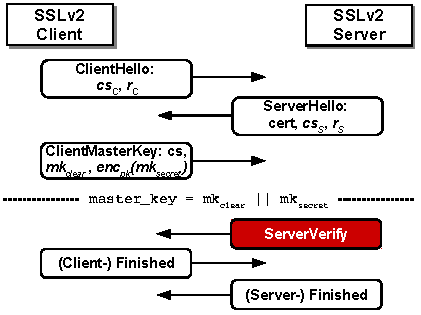
\includegraphics[width=\linewidth]{\DrownFigures/ssl-handshake} 
	\caption{\textbf{\ssltwo handshake.} The server responds with a \texttt{ServerVerify} message directly after receiving an RSA-\PKCS ciphertext contained in \texttt{ClientMasterKey}. This protocol feature enables our attack.\looseness=-1}
	\label{fig:ssl-handshake}
\end{figure}
%\fi
%
A client initiates an \ssltwo handshake by sending a
\texttt{ClientHello} message, which includes a list of cipher
suites $cs_c$ supported by the client and a client nonce $r_c$,
termed \texttt{challenge}.
The server responds with a \texttt{ServerHello} message, which
contains a list of cipher suites $cs_s$ supported by the server,
the server certificate, and a server nonce $r_s$, termed
$\texttt{connection\_ID}$.

The client responds with a \texttt{ClientMasterKey} message, which
specifies a cipher suite supported by both peers and key data
used for constructing a \texttt{master\_key}. In order to support
\textit{export} cipher suites with 40-bit security (e.g.,
\texttt{SSL\_RC2\_128\_CBC\_EXPORT40\_WITH\_MD5}), the key data is
divided into two parts:
\begin{itemize}
	\item $mk_{clear}$: A portion of the \texttt{master\_key} sent in the \texttt{ClientMasterKey} message as plaintext (termed \texttt{clear\_key\_data} in the \ssltwo standard).
	\item $mk_{secret}$: A secret portion of the
          \texttt{master\_key}, encrypted with RSA \PKCS (termed \texttt{secret\_key\_data}). 
\end{itemize}
The resulting \texttt{master\_key} $mk$ is constructed by
concatenating these two keys: $mk = mk_{clear} || mk_{secret}$. For
40-bit export cipher suites, $mk_{secret}$ is five bytes in length.
For non-export cipher suites, the whole \texttt{master\_key} is
encrypted, and the length of $mk_{clear}$ is zero.

The client and server can then compute session keys from the reconstructed \texttt{master\_key} $mk$:

\vspace{-6pt}
\begin{center}
\begin{math}
	\texttt{server\_write\_key} = MD5(mk || ``0" || r_c || r_s) \linebreak	
	\texttt{client\_write\_key} = MD5(mk || ``1" || r_c || r_s)
\end{math}
\end{center}
\vspace{-6pt}

The server responds with a \texttt{ServerVerify} message
consisting of the \texttt{challenge} $r_c$ encrypted with the
\texttt{server\_write\_key}.  Both peers then exchange
\texttt{Finished} messages in order to authenticate to each other.

Our attack exploits the fact that the server always decrypts an RSA-\PKCS
ciphertext, computes the \texttt{server\_write\_key}, and \textit{immediately}
responds with a \texttt{ServerVerify} message.  The \ssltwo standard
implies this message ordering, but does not make it explicit.
However, we observed this behavior in every implementation we
examined.  Our attack also takes advantage of the fact that the
encrypted $mk_{secret}$ portion of the \texttt{master\_key} can vary
in length, and is only five bytes for export ciphers.

% I Merged SSLv2 description and key derivation, ther were some redundancies ...

%\subsubsection{The SSLv2 key derivation mechanism}
%
%Recall that the RSA decryption code on the server decrypts the received RSA ciphertext, and checks the validity of the resulting plaintext as per the PKCS \#1 format. If the plaintext is valid, the server extracts from it the unpadded data, and uses that data, along with other information exchanged thus far during the protocol run, as the key for the chosen symmetric cipher. More formally:
%
%\begin{itemize}
%	\item Let the data from the decrypted RSA plaintext, after padding is removed, be termed \texttt{secret\_key\_data}.
%	\item Recall that the client and server have already exchanged a client nonce, termed \texttt{challenge} in the protocol standard, and a server nonce, termed $\texttt{connection\_ID}$.
%	\item Assume, as is the case throughout this work, that the chosen symmetric cipher is either export RC4 with a 128-bit key, of which 40 bits are secret, or export RC2 with the same key sizes\footnote{details vary slightly, but are very similar for other ciphers}. Then the client should send, along with the RSA ciphertext, a portion of the symmetric key in cleartext, termed \texttt{clear\_key\_data}, where \texttt{clear\_key\_data} is 11 bytes long. The sent \texttt{secret\_key\_data} should be exactly 5 bytes long. Let $\texttt{master\_key} = \texttt{clear\_key\_data} | \texttt{secret\_key\_data}$, where in this context $|$ refers to the concatenation operator.
%	\item Now let
%
%$\texttt{server\_write\_key} = MD5(\texttt{master\_key} | "0" | \texttt{challenge} | \texttt{connection\_ID})$
%
%$\texttt{client\_write\_key} = MD5(\texttt{master\_key} | "1" | \texttt{challenge} | \texttt{connection\_ID})$
%
%where the $|$ operator again means concatenation, and "0" and "1" refer to the corresponding ascii characters.
%
%	\item The respective keys are then used by each party both as keys for the chosen symmetric cipher, and as MAC keys.
%\end{itemize}

%As was hinted in the previous subsection, once an RSA key exchange with PKCS \#1 is implemented, the question immediately arises of how to act given an invalid RSA plaintext - recall that any observable difference in the treatment of invalid messages exposes a Bleichenbacher oracle to the attacker.
%Most implementations, including openssl, employ a counter-mechanism that has become somewhat standard: If the RSA plaintext is invalid or is of a wrong length, generate a random sequence of bytes of the expected length, and treat that sequence of bytes as if that was the plaintext after padding removal.
%
%As an aside, we note this counter-mechanism entails the risk of a timing attack: If the random byte sequence generation takes a measurable amount of time, an attacker may be able to observe the difference in processing times, and deduce the validity of the plaintext. Therefore, this counter-mechanism should be carefully implemented so as to require constant processing time. This is usually done by generating the random byte sequence before the RSA decryption, and choosing between the random sequence and the RSA plaintext according to the validity of the PKCS \#1 formatting. In fact, openssl's implementation of this mechanism was originally not constant-time for SSLv2, but the implementation was appropriately changed after we drew the maintainers' attention to this problem.



\ifsubmit\relax\else
\begin{figure}
	%\centering 
	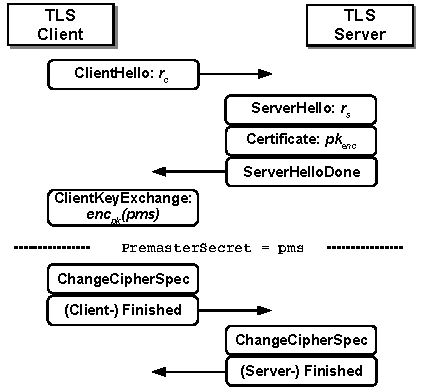
\includegraphics[width=\linewidth]{\DrownFigures/tls-handshake} 
	\caption{\textbf{TLS-RSA handshake.} After receiving an encrypted \pms, the server waits for an authenticated \texttt{ClientFinished} message.}
	\label{fig:tls-handshake}
\end{figure}
\fi

\paragraph{The TLS handshake protocol.}
In TLS~\cite{rfc5246} or \sslthree, the client initiates the handshake with a \texttt{ClientHello}, which contains a client random $r_c$ and a list of supported cipher suites. The server chooses one of the cipher suites and responds with three messages, \texttt{ServerHello}, \texttt{Certificate}, and \texttt{ServerHelloDone}. These messages include the server's choice of cipher suite, server nonce $r_s$, and a server certificate with an RSA public key. The client then uses the public key to encrypt a newly generated 48-byte \pms $pms$ and sends it to the server in a \texttt{ClientKeyExchange} message. The client and server then derive encryption and MAC keys from the \pms and the client and server random nonces. The details of this derivation are not important to our attack.  The client then sends \texttt{ChangeCipherSpec} and \texttt{Finished} messages. The \texttt{Finished} message authenticates all previous handshake messages using the derived keys. The server responds with its own \texttt{ChangeCipherSpec} and \texttt{Finished} messages.

The two main details relevant to our attacks are:
\begin{itemize}
	\item The \pms is always 48 bytes long, independent of the chosen cipher suite.  This is also true for export cipher suites.
	\item After receiving the \texttt{ClientKeyExchange} message, the server waits for the \texttt{ClientFinished} message, in order to authenticate the client.
\end{itemize}


\ifsubmit\relax\else
\subsubsection{Real-world protocol support}
TLSv1.0 is the most commonly supported protocol version, according to several surveys.  The SSL Labs SSL Pulse survey~\cite{ssllabs} reports that 98.6\% of about 140,000 popular TLS/SSL-enabled web sites supported TLSv1.0 in January 2016.  72.0\% supported TLSv1.2.  Support for \ssltwo was at 9.3\%, and \sslthree was at 29\%. Mayer et al.~\cite{DBLP:journals/corr/MayerZSH15} performed Internet-wide surveys of SMTP, IMAP, and POP3 between April and August 2015, and found that support for \ssltwo support was as high as 41.7\% of servers for SMTP on port 25 and as low as 3.7\% of IMAP servers on port 143.  Support for TLSv1.0 was nearly universal on these ports, varying from 91.6\% on port 25 to 98.9\% on port 143.

Bowen~\cite{bowencab} collected 213 million SSL/TLS client hellos and user agent strings from connections to popular sites, of which 183,000 (0.09\%) client hellos supported \ssltwo.  All of these client hellos also supported at least TLSv1.0.

Holz et al.~\cite{2016holz_analysis_tls-based_protocols_electronic_communication} performed passive monitoring to collect information about 16 million SSL/TLS connections during one week in July-August 2015.  They did not report any numbers for \ssltwo, and stated in personal communication that they did not observe any \ssltwo connections in their dataset.
\fi

%In response to our disclosure, OpenSSL has disabled \ssltwo by default in the 1.0.1r and 1.0.2f releases~\cite{opensslchangelog}.  

%This bug was also fixed in the aforementioned openssl releases.

\subsection{Bleichenbacher's attack}
\label{sec:bleichenbacher}
Bleichenbacher's attack is a padding oracle attack---it exploits the
fact that RSA ciphertexts should decrypt to \PKCS-compliant plaintexts.
If an implementation receives an RSA
ciphertext that decrypts to an invalid \PKCS plaintext, it might
naturally leak this information via an error message, by closing the
connection, or by taking longer to process the error condition.  This
behavior can leak information about the plaintext that can be modeled
as a cryptographic \textit{oracle} for the decryption
process. Bleichenbacher~\cite{Bleichenbacher} demonstrated how such an
oracle could be exploited to decrypt RSA ciphertexts.

%For example, the decrypting code may require different processing times for valid vs.\ invalid plaintexts - this is termed a "timing side-channel vulnerability". As another example, the decrypting code may send messages derived in some way from the plaintexts - this is termed a "direct message side channel vulnerability".
%The seminal work in this area \cite{Bleichenbacher} identified the general potential for such vulnerabilities, specifically using a direct message side channel vulnerability present in TLS implementations at the time, and demonstrated how such information could be gradually combined to eventually decrypt the RSA ciphertext in full.

\paragraph{Algorithm.}
In the simplest attack scenario, the attacker has a valid \PKCS
ciphertext $c_{0}$ that they wish to decrypt to discover the message
$m_{0}$.  They have no access to the private RSA key, but instead have
access to an oracle $\Oracle$ that will decrypt a ciphertext $c$ and
inform the attacker whether the most significant two bytes match
the required value for a correct \PKCS padding:
\begin{equation*} 
\Oracle(c) =  
\begin{cases} 
1 & \text{ if } m=c^d \bmod N \text{ starts with \hexb{00}{02}} \\ 
0 & \text{ otherwise.} 
\end{cases} 
\end{equation*} 

If the oracle answers with \texttt{1}, the attacker knows that $2B
\leq m \leq 3B-1$, where $B = 2^{8(\ell_m-2)}$.  The attacker can
take advantage of RSA malleability to generate new candidate ciphertexts
for any $s$:
\[
c = (c_{0} \cdot s^e) \bmod N = (m_{0} \cdot s)^e \bmod N 
\]
The attacker queries the oracle with $c$. If the oracle responds with
$0$, the attacker increments $s$ and repeats the previous
step. Otherwise, the attacker learns that for some~$r$, $2B \leq m_{0}s - rN  < 3B$. This allows the attacker to reduce the range of possible solutions to:  
\[ 
\frac{2B+rN}{s} \leq m_{0} < \frac{3B+rN}{s}  
\] 
The attacker proceeds by refining guesses for $s$ and $r$ values and
successively decreasing the size of the interval containing $m_{0}$.  At
some point the interval will contain a single valid value, $m_{0}$.
Bleichenbacher's original paper describes this process in further
detail~\cite{Bleichenbacher}.

\paragraph{Countermeasures.}
In order to protect against this attack, the decrypter must not leak
information about the \PKCS validity of the ciphertext.  The
ciphertext does not decrypt to a valid message, so the
decrypter generates a fake plaintext and continues the
protocol with this decoy.  The attacker should not be able to
distinguish the resulting computation from a correctly decrypted
ciphertext.

In the case of SSL/TLS, the server generates a random \pms to continue
the handshake if the decrypted ciphertext is
invalid.  The client will not possess the session key to send a valid
\texttt{ClientFinished} message and the connection will terminate.



\section{Breaking TLS with SSLv2}
In this section, we describe our cross-protocol DROWN attack that uses an
\ssltwo server as an oracle to efficiently decrypt TLS connections. The
attacker learns the session key for targeted TLS connections but does not
learn the server's private RSA key. We first describe our techniques using a
generic \ssltwo oracle. In Section~\ref{vulnerability}, we show how a
protocol flaw in \ssltwo can be used to construct such an oracle, and
describe our general DROWN attack. In Section~\ref{sec:special}, we show how
an implementation flaw in common versions of OpenSSL leads to a more powerful
oracle and describe our efficient special DROWN attack.

%\subsection{An efficient Bleichenbacher attack}

%\subsection{Attack scenario}
\label{sec:attack-scenario}

We consider a server accepting TLS connections from clients. The connections are established using a secure, state-of-the-art TLS version (1.0--1.2) and a \texttt{TLS\_RSA} cipher suite with a private key unknown to the attacker.

%\paragraph{Server RSA key exposed via \ssltwo.}
The same RSA public key as the TLS connections is also used for \ssltwo. For
simplicity, we will refer to the servers accepting TLS and \ssltwo
connections as the same entity.

%\paragraph{The attacker's position in the network.}
Our attacker is able to passively eavesdrop on traffic between the client and
server and record RSA-based TLS traffic.
The attacker may or may not be also required to perform active man-in-the-middle
interference, as explained below.

The attacker can expect to decrypt one out of 1,000 intercepted TLS
connections in our attack for typical parameters. This is a devastating
threat in many scenarios. For example, a decrypted TLS connection might
reveal a client's HTTP cookie or plaintext password, and an attacker would
only need to successfully decrypt a single ciphertext to compromise the
client's account. In order to collect 1,000 TLS connections, the attacker
might simply wait patiently until sufficiently many connections are recorded.
A less patient attacker might use man-in-the-middle interference, as in the
BEAST attack~\cite{beast-2011}.

\ifext
In order to collect 1,000 TLS connections, the attacker might simply wait patiently until sufficiently many connections are recorded.  If the attacker's intended victim is the \emph{server}, rather than a specific client, observing this many connections from many clients might take only a short time for an attacker who is located at a company firewall or who could perform a DNS spoofing or BGP hijacking attack to redirect traffic transparently through themselves.  If the attacker's intended victim is a \emph{particular client}, this is still feasible in many cases.  As an example, the Mozilla Thunderbird email client will check for new email messages every ten minutes by default.  A targeted user will make 1,000 connections after leaving the application running for a week.

A less patient attacker might have to resort to active man-in-the-middle techniques
in order to collect the required 1,000 TLS connections.
The attacker could embed or inject malicious JavaScript on an otherwise innocuous web site to cause the client to connect repeatedly to the victim server in a short time frame, as in the BEAST attack~\cite{beast-2011}.
The attacker may also need to trigger an error in each of the connections, in order
to prevent the handshakes from using TLS session resumption.
\fi


\subsection{A generic \ssltwo oracle}

Our attacks make use of an oracle that can be queried on a ciphertext and leaks information about the decrypted plaintext; this abstractly models the information gained from an \ssltwo server's behavior.  Our \ssltwo oracles reveal many bytes of plaintext, enabling an efficient attack.

Our cryptographic oracle $\Oracle$ has the following functionality: 
$\Oracle$ decrypts an RSA ciphertext $c$ and responds with ciphertext validity based on the decrypted message $m$.  
The ciphertext is valid only if $m$ starts with \hexb{00}{02} followed by non-null padding bytes, a delimiter byte \hex{00}, and a \texttt{master\_key} $mk_{secret}$ of correct byte length $\ell_k$.
We call such a ciphertext \textit{\sslconform}.

All of the \ssltwo padding oracles we instantiate give the attacker similar information about a \PKCSconform \ssltwo ciphertext:
\begin{equation*} 
\Oracle(c) =  
\begin{cases} 
mk_{secret} & \text{ if } c^d \bmod N = 00 || 02 || PS || 00 || mk_{secret}  \\ 
0 & \text{ otherwise.} 
\end{cases} 
\end{equation*}
That is, the oracle $\Oracle(c)$ will return the decrypted message $mk_{secret}$ if it is queried on a \PKCSconform \ssltwo ciphertext $c$ corresponding to a correctly \PKCS padded encryption of $mk_{secret}$.  The attacker then learns $\ell_k + 3$ bytes of $m = c^d \bmod N$: the first two bytes are $00 || 02$, and the last $\ell_k+1$ bytes are $00 || mk_{secret}$.  The length $\ell_k$ of $mk_{secret}$ varies based on the cipher suite used to instantiate the oracle.  For export-grade cipher suites such as \texttt{SSL\_RSA\_EXPORT\_WITH\_RC2\_CBC\_40\_MD5},
%or \texttt{SSL\_RSA\_EXPORT\_WITH\_RC4\_40\_MD5}\@,
$k$ will be 5 bytes, so the attacker learns 8 bytes of $m$.

\subsection{DROWN attack template}
\label{sec:adapted-bb-compact}
Our attacker will use an \ssltwo oracle $\Oracle$ to decrypt a TLS \texttt{ClientKeyExchange}.  
The behavior of $\Oracle$ poses two problems for the attacker. First, a TLS key exchange ciphertext decrypts to a 48-byte \pms. But since no \ssltwo cipher suites have 48-byte key strengths, this means that a valid TLS ciphertext is invalid to our oracle $\Oracle$. 
In order to apply Bleichenbacher's attack, the attacker must transform the TLS ciphertext into a valid \ssltwo key exchange message. Second, $\Oracle$ is very restrictive, since it strictly checks the length of the unpadded message. 
According to Bardou et al.~\cite{efficient-padding-oracle-2012}, Bleichenbacher's attack would require 12 million queries to such an oracle.\footnote{See Table~1 in~\cite{efficient-padding-oracle-2012}. The oracle is denoted with the term \texttt{FFF}.} 
%As each query would require an exhaustive search over $2^{40}$ values, this would make the attack significantly more costly.

Our attacker overcomes these problems by following this generic attack flow:
\begin{enumerate}
 \setcounter{enumi}{-1}
	\item The attacker collects many encrypted TLS RSA key exchange messages.
	\item The attacker converts one of the intercepted TLS ciphertexts containing a 48-byte \pms to an RSA \PKCS encoded ciphertext valid to the \ssltwo oracle $\Oracle$. \ifext We accomplish this by taking advantage of RSA ciphertext malleability and a technique of Bardou et al.~\cite{efficient-padding-oracle-2012}. \fi
	\item Once the attacker has obtained a valid \ssltwo RSA ciphertext, they can continue with a modified version of Bleichenbacher's attack, and decrypt the message after many more oracle queries.
	\item The attacker then transforms the decrypted plaintext back into the original plaintext, which is one of the collected TLS handshakes.
\end{enumerate}

We describe the algorithmic improvements we use to make each of these steps efficient below.

\subsubsection{Finding an \sslconform ciphertext}
\label{sec:trimmers}
The first step for the attacker is to transform the original TLS \texttt{ClientKeyExchange} message $c_0$ from a \tlsconform ciphertext into an \sslconform ciphertext. 
\ifext
A trivial approach would be to generate multipliers $s_i \in \{s_1,s_2,\ldots\}$, and compute ciphertexts $c_i = (c_0 {s_i}^e) \bmod N$, until one gets accepted by $\Oracle$.
However, the number of generated ciphertexts would be high, because $\Oracle$ is very restrictive; for 2048-bit RSA keys and an oracle expecting a 5-byte $mk_{secret}$ the probability that a random ciphertext becomes \sslconform is $P_{rnd} \approx (1/256)^3 * (255/256)^{249} \approx 2^{-25}$.
\fi

For this task, we rely on the concept of \emph{trimmers}, which were introduced by Bardou et al.~\cite{efficient-padding-oracle-2012}. 
Assume that the message $m_{0} = {c_0}^d \bmod N$ is divisible by a small number~$t$. In that case,  $m_{0} \cdot t^{-1} \bmod{N}$ simply equals the natural number $m_{0} / t$. 
If we choose $u \approx t$, and multiply the original message by $u \cdot t^{-1}$, the resulting number will lie near the original message: $m_0 \approx m_0 / t \cdot u$.  \ifext We shall refer to such fractions as ``small'' fractions. \fi

This method gives a good chance of generating a new \sslconform message. 
Let $c_0$ be an intercepted \tlsconform RSA ciphertext, and let $m_0 = c_0^d \bmod N$ be the \ifext corresponding \fi plaintext.  We select a multiplier $s = u/t \bmod N = u t^{-1} \bmod N$ where $u$ and $t$ are coprime, compute the value $c_1 = c_0 s^e \bmod N$, and query $\Oracle(c_1)$.  We will receive a response if $m_1 = m_0 \cdot u/t$ is \sslconform.  

As an example, let us assume a 2048-bit RSA ciphertext with $\ell_k = 5$, and consider the fraction $u = 7, t = 8$.  The probability that $c_0 \cdot u/t$ will be \sslconform is 1/7,774, so we expect to make 7,774 oracle queries before obtaining a positive response from $\Oracle$. Appendix~\ref{sec:fraction-probability} gives more details on computing these probabilities.

\subsubsection{Shifting known plaintext bytes}
\label{sec:rotations}
Once we have obtained an \sslconform ciphertext $c_1$, the oracle has also revealed the $\ell_k+1$ least significant bytes ($mk_{secret}$ together with the delimiter byte \hex{00}) and two most significant \hexb{00}{02} bytes of the \sslconform message $m_1$.  We would like to \emph{rotate} these known bytes around to the right, so that we have a large block of contiguous known most significant bytes of plaintext.
In this section, we show that this can be accomplished by multiplying by some shift $2^{-r} \bmod N$.  In other words, given an \sslconform ciphertext $c_1 = m_1^e \bmod N$, we can efficiently generate an \sslconform ciphertext $c_2 = m_2^e \bmod N$ where $m_2 = s \cdot m_1 \cdot 2^{-r} \bmod N$ and we know several most significant bytes of $m_2$. 

Let $R = 2^{8(k+1)}$ and $B = 2^{8(\ell_m-2)}$. Abusing notation slightly, let the integer $m_1 = 2 \cdot B + PS \cdot R + mk_{secret}$ be the plaintext satisfying $m_1^e = c_1 \bmod N$.  At this stage, the $\ell_k$-byte integer $mk_{secret}$ is known and the $\ell_m-\ell_k-3$-byte integer $PS$ is not.

Let $\tilde{m_1} = 2 \cdot B + mk_{secret}$ be the known components of $m_1$, so $m_1 = \tilde{m_1} + PS \cdot R$. We can use this to compute a new plaintext for which we know many most significant bytes.  Consider the value:
\[
m_1 \cdot R^{-1} \bmod N = \tilde{m_1} \cdot R^{-1} + PS \bmod N.
\]
The value of $PS$ is unknown and consists of $\ell_m-\ell_k-3$ bytes.  This means that the known value $\tilde{m_1} \cdot R^{-1}$ shares most of its $\ell_k+3$ most significant bytes with $m_1 \cdot R^{-1}$.

Furthermore, we can iterate this process by finding a new multiplier $s$ such that $m_2 = s \cdot m_1 \cdot R^{-1} \bmod N$ is also \sslconform.  A randomly chosen $s < 2^{30}$ will work with probability $2^{-25.4}$.  We can take use the bytes we have already learned about $m_1$ to efficiently compute such an $s$ with only 678 oracle queries in expectation for a 2048-bit RSA modulus.   Appendix~\ref{sec:rotation-details} gives more details.

\subsubsection{Adapted Bleichenbacher iteration}
\label{sec:bb-iteration}
It is feasible for all of our oracles to use the previous technique to entirely recover a plaintext message.  However, for our \ssltwo protocol oracle it is cheaper after a few iterations to continue using Bleichenbacher's original attack.  We can apply the original algorithm proposed by Bleichenbacher as described in Section~\ref{sec:bleichenbacher}\ifext, with minimal modifications\fi.

Each step obtains a message that starts with the required \hexb{00}{02} bytes after two queries in expectation.
Since we know the value of the $\ell_k+1$ least significant bytes after multiplying by any integer, we can query the oracle only on multipliers that cause the $(\ell_k+1)$st least significant byte to be zero.  However, we cannot ensure that the padding string is entirely nonzero; for a 2048-bit modulus this will hold with probability 0.37.

For a 2048-bit modulus, the total expected number of queries when using this technique to fully decrypt the plaintext is $2048 * 2 / 0.37 \approx 11,000$.


%\ifext
\begin{figure}[t]
	%\centering 
	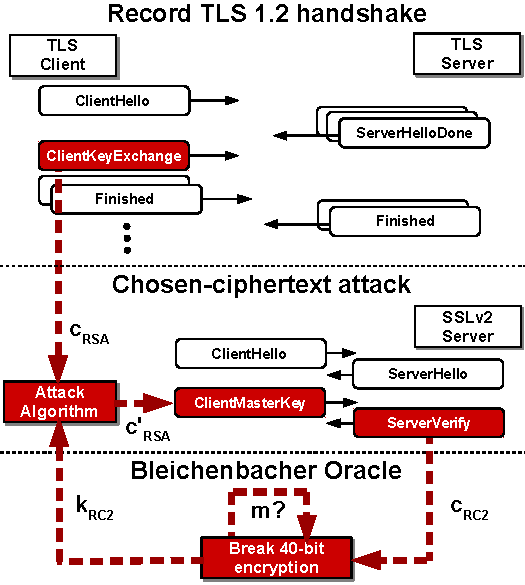
\includegraphics[width=\linewidth]{\DrownFigures/ssl-tls} 
	\caption{\textbf{\ssltwo-based Bleichenbacher attack on TLS}\,---\,%
	An attacker passively collects RSA ciphertexts from a TLS 1.2 handshake, and
    then performs oracle queries against a server that supports \ssltwo with the
	same public key to decrypt the TLS ciphertext.
	}
	\label{fig:ssl-tls}
\end{figure}
%\fi

\section{General DROWN} 
\label{vulnerability}

In this section, we describe how to use any correct \ssltwo implementation accepting export-grade cipher suites as a padding oracle.  We then show how to adapt the techniques described in Section~\ref{sec:adapted-bb-compact} to decrypt TLS RSA ciphertexts.

\subsection{The SSLv2 export padding oracle} 
\label{vulnerability}
\ssltwo is vulnerable to a direct message side channel vulnerability exposing a Bleichenbacher oracle to the attacker.
The vulnerability follows from three properties of \ssltwo.  First, the server immediately responds with a \texttt{ServerVerify} message after receiving the \texttt{ClientMasterKey} message, which includes the RSA ciphertext, without waiting for the \texttt{ClientFinished} message that proves the client knows the RSA plaintext.  Second, when choosing 40-bit export RC2 or RC4 as the symmetric cipher, only 5 bytes of the \texttt{master\_key} ($mk_{secret}$) are sent encrypted using RSA, and the remaining 11 bytes are sent in cleartext.  Third, a server
implementation that correctly implements the anti-Bleichenbacher countermeasure 
and receives an RSA key exchange message with invalid
padding will generate a random premaster secret and carry out the
rest of the TLS handshake using this randomly generated key material.

This allows an attacker to deduce the validity of RSA ciphertexts in the following manner:

\begin{enumerate}
	\item The attacker sends a \texttt{ClientMasterKey} message, which contains an RSA ciphertext $c_0$ and any choice of 11 clear key bytes for $mk_{clear}$. The server responds with a \texttt{ServerVerify} message, which contains the \texttt{challenge} encrypted using the \texttt{server\_write\_key}.
	\item The attacker performs an \textit{exhaustive search} over the possible values of the 5 bytes of the \texttt{master\_key} $mk_{secret}$, computes the corresponding \texttt{server\_write\_key}, and checks whether the \texttt{ServerVerify} message decrypts to \texttt{challenge}. One value should pass this check; call it $mk_0$. Recall that if the RSA plaintext was valid, $mk_0$ is the unpadded data in the RSA plaintext $c_0 ^d$. Otherwise, $mk_0$ is a randomly generated sequence of 5 bytes.
	\item The attacker re-connects to the server with the same RSA ciphertext $c_0$. The server responds with another \texttt{ServerVerify} message that contains the current \texttt{challenge} encrypted using the current \texttt{server\_write\_key}. If the decrypted RSA ciphertext was valid, the attacker can use $mk_0$ to decrypt a correct \texttt{challenge} value from the \texttt{ServerVerify} message. Otherwise, if the \texttt{ServerVerify} message does not decrypt to \texttt{challenge}, the RSA ciphertext was invalid, and $mk_0$ must have been random.
\end{enumerate}

Thus we can instantiate an oracle $\OracleSSLexp$ using the procedure above; each oracle query requires two server connections and $2^{40}$ decryption attempts in the simplest case.  For each oracle call $\OracleSSLexp(c)$, the attacker learns whether $c$ is valid, and if so, learns the two most significant bytes \hexb{00}{02}, the sixth least significant \hex{00} delimiter byte, and the value of the 5 least significant bytes of the plaintext $m$.

\ifext
If the server does not support 40-bit export ciphers, the attack can also be mounted in feasible computation time by choosing DES as the symmetric cipher.  Choosing DES means the exhaustive search is now done over a key space of 56 bits, thus increasing the cost of the attack by a factor of \begin{math} 2^{16} \end{math}, but does not fundamentally change anything except the increased cost.
\fi

\ifsubmit\relax\else
\subsection{OpenSSL special DROWN oracle}

We discovered a vulnerability present in OpenSSL versions prior to March 4, 2015 that allows a client to improperly provide cleartext key bytes for non-export ciphers.  Affected servers will substitute these bytes for bytes from the encrypted key.  This allows a client to successively learn a byte at a time of an encrypted key by brute forcing only 256 possibilities for each query. For a non-export 128-bit cipher suite such as \texttt{SSL\_RC4\_WITH\_MD5}, the attacker learns 19 bytes of the decrypted message.  We describe this vulnerability in more detail in Appendix~\ref{sec:clear-key-vuln}.  A client can then construct a Bleichenbacher oracle from this behavior by validating the \texttt{ServerVerify} message against the candidate key provided in the \texttt{clear\_key\_data}, resulting in no brute-force computation.
\fi

\subsection{TLS decryption attack}
\label{sec:bb-performance}

In this section, we describe how the oracle described in Section~\ref{vulnerability} can be used to carry out a feasible attack to decrypt passively collected TLS ciphertexts.

%\subsubsection{Attack scenario}
As described in Section~\ref{sec:attack-scenario}, we consider a server that accepts TLS connections from clients using an RSA public key that is exposed via \ssltwo, and an attacker who is able to passively observe these connections.

%\paragraph{Server supports export cipher suites for \ssltwo.}
We also assume the server supports export cipher suites for \ssltwo.
This can happen for two reasons.
First, the same server operators that fail to follow best practices in disabling \ssltwo~\cite{rfc6176} may also fail to follow best practices by supporting export cipher suites.
Alternatively, the server might be running a version of OpenSSL prior to January 2016, in which case it is vulnerable to the OpenSSL cipher suite selection bug described in Section~\ref{sec:openssl-selection}, and an attacker may negotiate a cipher suite of his choice independent of the server configuration.

% Nimrod: The previous subsection, introducing the generic SSLv2 oracle,
% already (implicitly) assumes this. Since we're short on space, I vote
% to remove this, at least for now.
\ifext
\paragraph{Correct Bleichenbacher countermeasure.}
We assume the server implements the recommended countermeasure against Bleichenbacher's attack in all protocol versions, including \ssltwo. If the decrypted RSA ciphertext has invalid padding, the server generates a random \pms or \texttt{master\_key} and continues the handshake with this random string. We assume this countermeasure is implemented correctly and the server is neither vulnerable to timing nor flush-and-reload side-channel attacks~\cite{Meyer14,Zhang:2014:CSA:2660267.2660356}.
\fi

%\paragraph{Computing power.}
The attacker needs access to computing power sufficient to perform a $2^{50}$ time attack, mostly brute forcing symmetric key encryption.  After our optimizations, this can be done with a one-time investment of a few thousand dollars of GPUs, or in a few hours for a few hundred dollars in the cloud.  Our cost estimates are described in~Section~\ref{sec:ec2_results}.

\if0
In our simplest attack scenario, an attacker is passively observing many connections between modern clients and server who negotiate a secure TLS version (1.0--1.2) with an RSA cipher suite and a well-generated, secure RSA public key.   The server is also configured to support \ssltwo with the same certificate as in TLS if a client requests it, although the modern victim clients will never negotiate \ssltwo.  The server implements the recommended countermeasures against Bleichenbacher attacks described in Section~\ref{sec:bleichenbacher}.



Our attacker will use our SSLv2 oracle $\OracleSSL$ to decrypt a TLS \texttt{ClientKeyExchange}.  We specialize the discussion below to our protocol-level oracle described in Section~\ref{vulnerability} and refer to this attack as the \emph{general} DROWN attack.  The adaptations to the OpenSSL clear-key oracle, which produces our faster \emph{special} DROWN attack are similar and are described in Section~\ref{sec:special}.
\fi

\subsubsection{Constructing the attack}

The attacker can exploit the \ssltwo vulnerability
\ifext as illustrated in Figure~\ref{fig:ssl-tls}, \fi
following the generic attack outline described in Section~\ref{sec:adapted-bb-compact},
consisting of several distinct phases:

\begin{enumerate}
 \setcounter{enumi}{-1}
	\item The attacker passively collects 1,000 TLS handshakes from
	connections using RSA key exchange.

	\item They then attempt to convert the intercepted TLS ciphertexts containing a 48-byte \pms to valid RSA \PKCS encoded ciphertexts containing five-byte messages using the fractional trimmers described in Section~\ref{sec:trimmers}, and querying $\OracleSSLexp$. The attacker sends the modified ciphertexts to the server using fresh \ssltwo connections with weak symmetric ciphers and uses the \texttt{ServerVerify} messages to deduce ciphertext validity as described in the previous section. For each queried RSA ciphertext, the attacker must perform a brute force attack on the weak symmetric cipher. The attacker expects to obtain a valid \ssltwo ciphertext after roughly 10,000 oracle queries, or 20,000 connections to the server.

	\item Once the attacker has obtained a valid \ssltwo RSA ciphertext
	$c_1 = m_1^e$, they use the shifting technique explained in
	Section~\ref{sec:rotations} to find an integer $s_1$ such that
	$m_2 = m_1 \cdot 2^{-40} \cdot s_1$ is also \sslconform.
	Appendix~\ref{sec:general-rotations} contains more details on this step.

	\item The attacker then applies the shifting technique again to find
	another integer $s_2$ such that $m_3 = m_2 \cdot 2^{-40} \cdot s_2$
	is also \sslconform.

	\item They then search for yet another integer $s_3$ such that
	$m_3 \cdot s_3$ is also \sslconform.

	\item Finally, the attacker can continue with our adapted Bleichenbacher
	iteration technique described in Section~\ref{sec:bb-iteration}, and
	decrypts the message after an expected 10,000 additional oracle queries,
	or 20,000 connections to the server.

	\item The attacker can then transform the decrypted plaintext back into
	the original plaintext, which is one of the 1,000 intercepted TLS 		handshakes.

\end{enumerate}

\paragraph{The rationale behind the different phases.}
Bleichenbacher's original algorithm requires a conformant message $m_0$, and a multiplier $s_1$ such that $m_1 = m_0 \cdot s_1$ is also conformant.
Na\"{\i}vely, it would appear we can apply the same algorithm here, after completing Phase 1.
However, the original algorithm expects $s_1$ to be of size about $2^{24}$. This is not the case when we use fractions for $s_1$, as the integer $s_1 = u t^{-1} \bmod N$ will be the same size as $N$.

Therefore, our approach is to find a conformant message for which we know the 5 most significant bytes; this will happen after multiple rotations and
this message will be $m_3$.
After finding such a message, finding $s_3$ such that $m_4 = m_3 \cdot s_3$ is also conformant becomes trivial.
From there, we can finally apply the adapted Bleichenbacher iteration technique as described in Appendix~\ref{sec:general-bleichenbacher}.

\begin{table}[t]
  \centering
	\begin{tabular}{rrrrrr}
	\toprule
	\textbf{Optimizing} & \textbf{Cipher-} & \textbf{$|F|$}     & \textbf{\ssltwo}  & \textbf{Offline} \\
        \textbf{for}        & \textbf{texts}   &           & \textbf{connections} & \textbf{work} \\
	\midrule
	offline work        &           12,743 &          1 &            50,421  & $2^{49.64}$ \\
        offline work        &            1,055 &         10 &              46,042  & $2^{50.63}$ \\
	% compromise is achieved by using fractions {8/7, 8/9}; numbers are now final
       	compromise          &            4,036 &          2 &              41,081  & $2^{49.98}$ \\
	online work         &            2,321 &          3 &              38,866  & $2^{51.99}$ \\
	online work         &              906 &          8 &              39,437  & $2^{52.25}$ \\
	\bottomrule
	\end{tabular}
		\caption{\textbf{2048-bit Bleichenbacher attack complexity}\,---\,%
		The cost to decrypt one ciphertext can be adjusted by choosing the set of
        fractions $F$ the attacker applies to each of the passively collected
		ciphertexts in the first step of the attack. This choice affects several
		parameters: the number of these collected ciphertexts, the number of
 		connections the attacker makes to the \ssltwo server, and the number of
		offline decryption operations.
		}
        \label{tab:reasonable_parameters}
\end{table}

\begin{table}[t]
\begin{tabular*}{\linewidth}{@{\extracolsep{\fill}\hskip\tabcolsep}rrrrr}
\toprule
\textbf{Key size}    & \textbf{Phase 1} & \textbf{Phases 2--5} & \textbf{Total}   & \textbf{Offline} \\
                     &                 &                 & \textbf{queries} & \textbf{work}    \\
\midrule
% This is all when using 4/5, which has a maximal "native probability" of 0.1.
% Offline work is always step1 * 2**38
%              1024 &  (0.1 * 0.62 * 1/256)**(-1)  & + 256 / 0.62 * 2 + 2/0.62 + 1024 * 2 / 0.62
               1024 &  4,129   &  4,132  &  8,261 & $2^{50.01}$ \\

%              2048 & (0.1 * 0.37 * 1/256)**(-1)   & + (2.72 * 2**8) * 2 + 2.72*2 + 2048 * 2 / 0.37 (number for phase 5 also matches runs)
               2048 &  6,919   &  12,468 & 19,387 & $2^{50.76}$ \\

%              4096 & (0.1 * 0.14 * 1/256)**(-1)   & + 2**8 / 0.14 * 2 + 2/0.14 + 4096 * 2 / 0.14
               4096 &  18,286  &  62,185 & 80,471 & $2^{52.16}$ \\
\bottomrule
\end{tabular*}
	\caption{\textbf{Oracle queries required by our attack}\,---\,%
	In Phase 1, the attacker queries the oracle until an \ssltwo conformant
	ciphertext is found. In Phases 2--5, the attacker decrypts this ciphertext
	using leaked plaintext. These numbers minimize total queries. In our attack,
	an oracle query represents two server connections.
	}
	\label{tab:optimal_queries}
\end{table}

\newcommand{\GPUTable}{
\begin{table*}[t]
 \centering
 \begin{tabular}{llrrrr}
        \toprule
        \textbf{Platform} & \textbf{Hardware} & \textbf{Cost} & \textbf{Full attack}  & \textbf{Cost to perform attack in 1 day} \\
        \midrule
        Na\"{\i}ve CPU & 4 Intel Xeon E7-4820 & $\$21,400$ & $114$ days  & \$$2,440,000$\\
        Na\"{\i}ve GPU & ZOTAC GeForce GTX TITAN & $\$2,400$  & $189$ days & \$$450,000$ \\
        Na\"{\i}ve FPGA & 64 Spartan-6 LX150 & $\$60,000$ & $51.5$ days  & \$$3,090,000$  \\
        \cmidrule{1-5}
        Optimized Hashcat & NVIDIA GTX / AMD R9 & \$18,040 & $0.75$ days & \$13,500 \\
        Optimized EC2 & NVIDIA & \$440 & $0.33$ days & \$147 \\
        \bottomrule
    \end{tabular}	
	\caption{\textbf{Time and cost efficiency of our attack on different hardware platforms.}\,---\,%
	The brute force attacks against symmetric export keys are the most expensive
	part of our attack. We compared the performance of a na\"{\i}ve
	implementation of our attack on different platforms, and decided that a GPU
	implementation held the most promise. We then heavily optimized our GPU
	implementation, obtaining several orders of magnitude in speedup.
	}
\label{perf_comparison}
\end{table*}
}

\subsubsection{Attack performance}
The attacker wishes to minimize three major costs in the attack: the number of recorded ciphertexts from the victim client, the number of connections to the victim server, and the number of symmetric keys to be brute forced.
The requirements for each of these elements are governed by the set of fractions to be multiplied with each RSA ciphertext in the first phase, as described in Section~\ref{sec:trimmers}.

Table~\ref{tab:reasonable_parameters} highlights a few choices for $F$ and the resulting performance metrics for 2048-bit RSA keys.
Appendix \ref{sec:adapted-bb} provides more details on the derivation of these numbers and other optimization choices.
Table \ref{tab:optimal_queries} gives the expected number of Bleichenbacher queries for different RSA key sizes, when minimizing total oracle queries.

%These are fractions of small coprime numbers, similar to the example $u/t = 8/7$, and ideally amenable to the additional optimization described above.





%The special DROWN attack requires similar numbers of ciphertexts and oracle queries, but the amount of computation is negligible.




\subsection{Implementing general DROWN with GPUs} 
%% In the following section, we experimentally evaluate the cost of brute forcing export \texttt{master\_key} values on CPU, GPU, FPGA, and cloud computing platforms. 
%% We then experimentally evaluate our general DROWN attack using the 
%% \texttt{SSL\_RC2\_128\_CBC\_EXPORT40\_WITH\_MD5}
%% cipher suite, which is the most suitable for this attack.

%% \subsubsection{Comparing hardware platforms}
\if0
The most computationally expensive part of our general DROWN attack is breaking the 40-bit symmetric key.  We wanted to find the platform that would have the best tradeoff of cost and speed for the attack, so we performed some preliminary experiments comparing performance of symmetric key breaking on CPUs, GPUs, and FPGAs.  These experiments used a na\"{\i}ve version of the attack using the OpenSSL implementation of MD5 and RC2.

The CPU machine contained four Intel Xeon E7-4820 CPUs with a total of 32 cores (64 concurrent threads). The GPU system was equipped with a ZOTAC GeForce GTX TITAN and an Intel Xeon E5-1620 host CPU\@. The FPGA setup consisted of 64 Spartan-6 LX150 FPGAs.

We benchmarked the performance of the CPU and GPU implementations over a large corpus of randomly generated keys, and then extrapolated to the full attack.
For the FPGAs, we tested the functionality in simulation and estimated the actual runtime by theoretically filling the FPGA up to 90\% with the design, including communication.
Table~\ref{perf_comparison} compares the three platforms.

While the FPGA implementation was the fastest in our test setup, the speed-to-cost ratio of GPUs was the most promising. Therefore, we decided to focus on optimizing the attack on the GPU platform.
\fi

\ifext
\subsubsection{Optimized GPU implementation}
\label{sec:gpu_brief}
We developed a highly optimized GPU implementation of our general DROWN brute force attack.  Our first na\"{\i}ve GPU implementation performed around 26MH/s, where MH measures the calculation of an MD5 hash and the RC2 decryption. The optimizations described below gave a final speed of 515MH/s, a speedup factor of 19.8.
\fi

\ifext
We obtained our improvements through a number of optimizations.  Our original implementation ran into a communication bottleneck in the PCI-E bus in transmitting candidate keys from CPU to GPU, so we removed this bottleneck by generating key candidates on the GPU itself.  We optimized memory management, including storing candidate keys and the RC2 permutation table in constant memory, which is almost as fast as a register, instead of slow global memory.  We optimized the cryptographic checks themselves by rewriting the RC2 implementation to use 32-bit instructions, removing unnecessary RC2 keysize checks, dropping unused ADD instructions during MD5, and manually shifting input bytes into the MD5 input registers to avoid loop branches.
\looseness=1
\fi

\ifext

\label{sec:ec2_results}
%In this section, we discuss attack performance and cost when a rented cloud compute cluster is used for the GPU breaking.
\fi

The most computationally expensive part of our general DROWN attack is breaking the 40-bit symmetric key, so we developed a highly optimized GPU implementation of this brute force attack.  Our first na\"{\i}ve GPU implementation performed around 26MH/s, where MH denotes the time required for testing one million possible values of $mk_{secret}$. Our optimized implementation runs at a final speed of 515MH/s, a speedup factor of 19.8.  
\label{sec:gpu_brief}

We obtained our improvements through a number of optimizations.  For example, our original implementation ran into a communication bottleneck in the PCI-E bus in transmitting candidate keys from CPU to GPU, so we removed this bottleneck by generating key candidates on the GPU itself.  We optimized memory management, including storing candidate keys and the RC2 permutation table in constant memory, which is almost as fast as a register, instead of slow global memory. 
\ifext  We optimized the cryptographic checks themselves by rewriting the RC2 implementation to use 32-bit instructions, removing unnecessary RC2 keysize checks, dropping unused ADD instructions during MD5, and manually shifting input bytes into the MD5 input registers to avoid loop branches.  We describe these optimizations in further detail in Appendix~\ref{sec:gpu}. \fi

We experimentally evaluated our optimized implementation on a local cluster and in the cloud.
We used it to execute a full attack of $2^{49.6}$ tested keys on each platform.
The required number of keys to test during the attack is a random variable, distributed geometrically, with an expectation that ranges between $2^{49.6}$ and $2^{52.5}$ depending on the choice of optimization parameters.
We treat a full attack as requiring $2^{49.6}$ tested keys overall.

\paragraph{Hashcat.}
Hashcat~\cite{hashcat} is an open source optimized password-recovery tool.
The Hashcat developers allowed us to use their GPU servers for our attack evaluation. 
The servers contain a total of 40 GPUs: 32 Nvidia GTX 980 cards, and 8 AMD R9 290X cards.
The value of this equipment is roughly \$18,040.
Our full attack took less than 18 hours to complete on the Hashcat servers, with the longest single instance taking 17h9m.

% Nimrod: Generally, we can't report times which are different from wallclock times without further explanation,
% like "retroactively assuming a perfecly balanced distribution..."
% The instance that took longest took 1029m41.176, which is 17.16 hours,
% so I think any number smaller than 18 hours would need to be discussed.

\paragraph{Amazon EC2.}
\label{sec:ec2_results}
% AH: Suggest trimming this as in the submitted version
\ifext
% !TEX root = ../../../proposal.tex
%\section{Brute Forcing Keys with Amazon EC2} 
\label{sec:ec2-details}

%Amazon Elastic Cloud Compute (EC2)~\cite{ec2} is a service that provides on-demand virtualized compute resources to customers. 
%This is an affordable alternative to provisioning one's own local cluster.

Amazon EC2 billing is based on the \textit{instance-hour}. An \textit{instance} represents a single virtualized machine and its associated cores, memory, and storage. For our experiments we used \texttt{g2} instances, which are equipped with high-performance NVIDIA GPUs, each with 1,536 CUDA cores. The two available models for this instance type are the \texttt{g2.2xlarge} and the \texttt{g2.8xlarge}, containing one and four GPUs, respectively.

It is possible to request instances at a fixed on-demand rate, or bid on instances at the discounted spot instance rate. Spot instances may be terminated depending on demand, but the savings in cost are significant compared to the on-demand rate. 
When we ran our experiments in January 2016, the on-demand rate for the \texttt{g2.2xlarge} model was \$0.65/hr and the rate for the \texttt{g2.8xlarge} model was \$2.65/hr, while the average spot rates we paid were \$0.09/hr and \$0.83/hr respectively.

We used a cluster composed of 200 spot instances: 150 \texttt{g2.2xlarge} which contain one GPU and 50 \texttt{g2.8xlarge}, each containing four GPUs, spread across multiple availability zones within the US-East region.
This distribution was determined by price: we were not able to launch more than 50 \texttt{g2.8xlarge} instances without a sharp spike in spot prices. We used the optimized Hashcat implementation on the same workload of key requests as the experiments run on the Hashcat servers.  We used Slurm~\cite{yoo2003slurm} to distribute jobs across compute nodes.

The GPU breaking experiment completed successfully, with two minor caveats. First, the 150 \texttt{g2.2xlarge} nodes completed their workloads at the 6h26m mark, while the other 50 \texttt{g2.8xlarge} nodes did not finish until the 7h41m mark. More careful job distribution would ensure that all nodes completed at approximately the same time, reducing the overall runtime. Second, in this particular run, $7.2\%$ of the jobs that we expected to complete were terminated early due to overheating GPUs.  The attack was successful despite the failed jobs, so we did not rerun them. In a more carefully engineered implementation, the unfinished jobs could have been reallocated to the unused GPU capacity without increasing the overall runtime.

The total cost of the experiment was \$440, and terminated in under 8 hours including startup and shutdown.


\else
We also ran our optimized GPU code on the Amazon Elastic Compute Cloud (EC2) service.  We used a cluster composed of 200 variable-price ``spot'' instances: 150 \texttt{g2.2xlarge} instances, each containing one high-performance NVIDIA GPU with 1,536 CUDA cores and 50 \texttt{g2.8xlarge} instances, each containing four of these GPUs.  
When we ran our experiments in January 2016, the average spot rates we paid were \$0.09/hr and \$0.83/hr respectively.  
%The 150 \texttt{g2.2xlarge} nodes finished after 6h26m, while the \texttt{g2.8xlarge} finished after 7h41m.  $7.2\%$ of the jobs that we expected to complete failed due to overheating GPUs.  The attack was successful despite the failed jobs, so we did not rerun them.  
Our full attack finished in under 8 hours including startup and shutdown for a cost of \$440.  
\ifext See Appendix~\ref{sec:ec2-details} for more details. \fi
\fi


\subsection{OpenSSL SSLv2 cipher suite selection bug}

General DROWN is a protocol flaw, but the population of vulnerable hosts is
increased due to a bug in OpenSSL that causes many servers to erroneously
support \ssltwo and export ciphers even when configured not to. The OpenSSL
team intended to disable \ssltwo by default in 2010, with a change that removed
all \ssltwo cipher suites from the default list of ciphers offered by the
server~\cite{openssl-changelog}.  However, the code for the protocol itself was
not removed in standard builds and \ssltwo itself remained enabled. We
discovered a bug in OpenSSL's \ssltwo cipher suite negotiation logic that
allows clients to select \ssltwo cipher suites even when they are not
explicitly offered by the server. We notified the OpenSSL team of this
vulnerability, which was assigned CVE-2015-3197.  The problem was fixed in
OpenSSL releases 1.0.2f and 1.0.1r~\cite{openssl-changelog}.
%\looseness=1


\section{Special DROWN}
\label{sec:special}

We discovered a vulnerability in recent
(but not current) versions of the OpenSSL SSLv2 handshake code that
creates a powerful Bleichenbacher oracle, and drastically reduces the amount
of computation required to implement our attack.  
The vulnerability, which has been designated CVE-2016-0703, was
present in the OpenSSL codebase from at least the start of the repository,
in 1998, until it was unknowingly fixed on March 4, 2015 by a
patch~\cite{openssl-clear-patch} designed to correct an unrelated
problem~\cite{CVE-2015-0293}.
By adapting DROWN to
exploit this special case, we can cut the number of connections
required by more than 50\% and reduce the computational work to a negligible amount.

%To distinguish the two, we call the attack developed so far
%\emph{general} DROWN and refer to the variant that
%exploits the OpenSSL bug as \emph{special} DROWN\@.  General DROWN is
%a protocol-level attack that makes few assumptions about the SSLv2
%server, other than that it allows export cipher handshakes.  Special
%DROWN exploits a specific implementation bug, but it is highly practical.
%It may be the first widespread Bleichenbacher vulnerability within reach of ``script-kiddies'' and other low-resource
%attackers.

%% This dramatic discovery came too late to fully incorporate into the
%% body of our submission, so for now we confine the bulk of the
%% discussion to this section.

% !TEX root = ../../../proposal.tex
\subsection{The OpenSSL ``extra clear'' oracle}

%\subsubsection{A key recovery attack on SSLv2 handshakes}

\label{sec:clear-key-vuln}

Prior to the fix, OpenSSL servers improperly allowed the \texttt{ClientMasterKey} message to contain
\texttt{clear\_key\_data} bytes for \emph{non-export} ciphers.  When such bytes are present,
the server substitutes them for bytes from the
encrypted key. For example, consider the case that the client chooses a 128-bit cipher and sends a 16-byte
encrypted key $k\pos{1}, k\pos{2}, \ldots, k\pos{16}$ but, contrary to the protocol specification, includes 4
null bytes of \texttt{clear\_key\_data}. Vulnerable OpenSSL versions will
construct the following \texttt{master\_key}:

\small $[00\ 00\ 00\ 00\ k\pos{1}\ k\pos{2}\ k\pos{3}\ k\pos{4}\ \dots\ k\pos{9}\ k\pos{10}\ k\pos{11}\ k\pos{12}]$\normalsize

This enables a straightforward key recovery attack against such versions.
An attacker that has intercepted an \ssltwo connection takes the RSA
ciphertext of the encrypted key and replays it in non-export handshakes to
the server with varying lengths of \texttt{clear\_key\_data}. For a 16-byte
encrypted key, the attacker starts with 15 bytes of clear key, causing the server to use the \texttt{master\_key}:

\small$[00\ 00\ 00\ 00\ 00\ 00\ 00\ 00\ 00\ 00\ 00\ 00\ 00\ 00\ 00\ k\pos{1}]$\normalsize

The attacker can brute force the first byte of the encrypted key by
finding the matching \texttt{ServerVerify} message among 256
possibilities. Knowing $k\pos{1}$, the attacker makes another
connection with the same RSA ciphertext but 14 bytes of clear key,
resulting in the \texttt{master\_key}:

\small $[00\ 00\ 00\ 00\ 00\ 00\ 00\ 00\ 00\ 00\ 00\ 00\ 00\ 00\ k\pos{1}\ k\pos{2}]$\normalsize

% Note: The number below is 15, since you the original intercepted connection
% servers as the case with 0 bytes of clear_key_data.
The attacker can now easily brute force $k\pos{2}$. With only 15 probe
connections and an expected $15 \cdot 128 = 1,920$
trial encryptions, the attacker learns the entire \texttt{master\_key} for the
recorded session.

%\subsubsection{An improved oracle for DROWN}

As this oracle is obtained by improperly sending unexpected clear-key bytes,
we call it the Extra Clear oracle.

This session key-recovery attack can be directly converted to a Bleichenbacher oracle. Given a candidate ciphertext and symmetric key length $\ell_k$, the attacker sends the ciphertext with $\ell_k$ known bytes of \texttt{clear\_key\_data}. The oracle decision is simple:
\begin{itemize}
\item If the ciphertext is valid, the \texttt{ServerVerify} message will reflect a \texttt{master\_key} consisting of those $\ell_k$ known bytes.
\item If the ciphertext is invalid, the \texttt{master\_key} will be replaced with $\ell_k$ random bytes (by following the countermeasure against the Bleichenbacher attack), resulting in a different \texttt{ServerVerify} message.
\end{itemize}

This oracle decision requires one connection to the server and one \texttt{ServerVerify} computation. After the attacker has found a valid ciphertext corresponding to a $\ell_k$-byte encrypted key, they recover the $\ell_k$ plaintext bytes by repeating the key recovery attack from above.  Thus our oracle $\OracleSSLclear(c)$ requires one connection to determine whether $c$ is valid.  After $\ell_k$ connections, the attacker additionally learns the $\ell_k$ least significant bytes of $m$.  We model this as a single oracle call, but the number of server connections will vary depending on the response.


\tabDrownAll

\subsection{TLS decryption with special DROWN}
\label{sec:clear_analysis}

Using our oracle $\OracleSSLclear$, we can construct an extremely efficient version of our TLS decryption attack.  The OpenSSL \tOracleSSLclear provides three significant advantages over our export oracle $\OracleSSLexp$: (1) It no longer requires an export cipher suite, and, in fact, we gain efficiency by exploiting regular SSLv2 ciphers; (2) It requires only one handshake per oracle query; and (3) Computation is reduced to one \texttt{ServerVerify} decryption per oracle query, versus $2^{40}$.

\subsubsection{Attack scenario}

As before, we consider a server that accepts TLS connections, and a client that negotiates a secure, state-of-the-art TLS version with a \texttt{TLS\_RSA} cipher suite.  The same RSA key pair used for TLS is also used on a server that is running a vulnerable version of OpenSSL.

\subsubsection{Constructing the attack}

The attacker can exploit the OpenSSL extra clear vulnerability to efficiently decrypt a TLS ciphertext as follows.  We will use the cipher suite \texttt{SSL\_DES\_192\_EDE3\_CBC\_WITH\_MD5} as the cipher suite, allowing the attacker to recover 24 bytes of key at a time from the oracle.
We first present a straightforward adaptation of the general DROWN attack to the \tOracleSSLclear,
before later applying a few additional optimizations made possible by this new oracle.

\begin{enumerate}
 \setcounter{enumi}{-1}
 \item The attacker intercepts several hundred TLS handshakes using RSA key exchange.
 \item The attacker uses the fractional trimmers as described in Section~\ref{sec:trimmers} to convert the TLS ciphertexts into an \sslconform ciphertext $c_0$.
 \item Once the attacker has obtained a valid \ssltwo ciphertext $c_1$, he repeatedly uses the shifting technique described in Section~\ref{sec:rotations} to rotate the message by 25 bytes each iteration, learning 27 bytes with each shift.  After several iterations, he has learned the entire plaintext.
 \item The attacker then transforms the decrypted \ssltwo plaintext into the decrypted TLS plaintext. 
 \end{enumerate}

\paragraph{Attack costs}
Using 40 fractional trimmers, this more efficient oracle attack allows
the attacker to recover one in 260 TLS session keys using only about
17,000 connections to the server.  The computation cost is so low that
we can complete the full attack on a single workstation in under one
minute. Appendix~\ref{sec:special-performance} gives more details.

Mounting the attack using the optimized version of Special DROWN
described in Appendix~\ref{sec:special-performance} allows the
attacker to target one of 100 connections, at the expense of
increasing the number of queries to 27,000.

\subsection{MITM attack against TLS}

Special DROWN is fast enough that it can decrypt a TLS premaster
secret \emph{online}, during a connection handshake.  A
man-in-the-middle attacker can use it to compromise connections
between modern browsers and TLS servers---even those configured to
prefer non-RSA cipher suites.

\paragraph{Attack scenario.}
The MITM attacker impersonates the server and sends a
\texttt{ServerHello} message that selects a cipher suite with RSA as
the key-exchange method.  Then, the attacker uses special DROWN to
decrypt the \pms.  The main difficulty is completing the decryption and producing a valid
\texttt{ServerFinished} message before the client's connection times
out.  Most browsers will allow the handshake to last up to one minute~\cite{LogJam}.

Using the fully optimized version of special DROWN, the attack still requires intercepting 
an average of 100 ciphertexts, only one of
which will be decrypted, probabilistically.  The simplest
way for the attacker to facilitate this is to use JavaScript to cause
the client to connect repeatedly to the victim server, as described in
Section~\ref{sec:attack-scenario}.  Each connection is tested
against the oracle with only small number of fractions, and the attacker can discern
immediately when he receives a positive response from the oracle.

Once the attacker has obtained a positive response, he
can proceed to the final phase of the special DROWN attack described above, 
which employs 200-bit rotation 10 times to fully decrypt the
plaintext.   Our current implementation requires under
30 seconds for this phase on a single PC.

% AH: The 34 microsecond number for 2048-bit RSA doesn't seem right.
% Here's a trial with openssl on a fairly modern server:
%
%% $ openssl speed rsa
%% Doing 512 bit private rsa's for 10s: 176064 512 bit private RSA's in 10.00s
%% Doing 512 bit public rsa's for 10s: 2092137 512 bit public RSA's in 10.00s
%% Doing 1024 bit private rsa's for 10s: 53091 1024 bit private RSA's in 10.00s
%% Doing 1024 bit public rsa's for 10s: 779785 1024 bit public RSA's in 10.00s
%% Doing 2048 bit private rsa's for 10s: 7199 2048 bit private RSA's in 10.00s
%% Doing 2048 bit public rsa's for 10s: 234671 2048 bit public RSA's in 10.00s
%% Doing 4096 bit private rsa's for 10s: 1005 4096 bit private RSA's in 10.01s
%% Doing 4096 bit public rsa's for 10s: 63173 4096 bit public RSA's in 10.01s

% Nimrod: Let's go with your number then.
% Just for the record, I got the number from the QUIC Crypto document:
% https://docs.google.com/document/d/1g5nIXAIkN_Y-7XJW5K45IblHd_L2f5LTaDUDwvZ5L6g/edit#heading=h.bzxklo2i5w6k

The ability of the victim server to perform 17,000 handshakes in less than a
minute is not an impediment for modern hardware.  An RSA
private key operation with a 2048-bit modulus requires on the order of
1~ms using OpenSSL on a recent-generation CPU, so the cryptographic
portion of the attacker's queries induces additional server load of
roughly 14~core-seconds.  In tests with a nearby server running Apache
2.4, we could easily complete 10,000 HTTPS requests in under 10
seconds.

% AH: Here's further data in support of this fact, tested against a local
% server.  10k TLS/RSA connections took about 7 seconds to complete.

%% $ ab -n 10000 -c 100 -Z AES128-SHA https://www.eecs.umich.edu/x
%% This is ApacheBench, Version 2.3 <$Revision: 1528965 $>
%% Copyright 1996 Adam Twiss, Zeus Technology Ltd, http://www.zeustech.net/
%% Licensed to The Apache Software Foundation, http://www.apache.org/

%% Benchmarking www.eecs.umich.edu (be patient)

%% Server Software:        Apache/2.2.15
%% Server Hostname:        www.eecs.umich.edu
%% Server Port:            443
%% SSL/TLS Protocol:       TLSv1.2,AES128-SHA,2048,128

%% Document Path:          /x
%% Document Length:        285 bytes

%% Concurrency Level:      100
%% Time taken for tests:   7.130 seconds
%% Complete requests:      10000
%% Failed requests:        0
%% Non-2xx responses:      10000
%% Total transferred:      4660000 bytes
%% HTML transferred:       2850000 bytes
%% Requests per second:    1402.45 [#/sec] (mean)
%% Time per request:       71.304 [ms] (mean)
%% Time per request:       0.713 [ms] (mean, across all concurrent requests)
%% Transfer rate:          638.22 [Kbytes/sec] received

%% Connection Times (ms)
%%               min  mean[+/-sd] median   max
%% Connect:       28   57  47.7     52    1069
%% Processing:     7   13   7.2     13     234
%% Waiting:        7   12   7.2     12     230
%% Total:         47   70  48.1     65    1082






% !TEX root = ../../../proposal.tex
%In addition to the \tOracleSSLclear $\OracleSSLclear$ described in Section~\ref{sec:special},
%the same set of OpenSSL versions allow a different oracle,
%which we term \tOracleSSLleaky $\OracleSSLleaky$.
%This additional oracle is powerful in a different way than
%\tOracleSSLclear --- it still requires roughly $2^{40}$ offline computations
%per query, but it is more permissive when checking for conformant messages.

\subsection{The OpenSSL ``leaky export'' oracle}
In addition to the extra clear implementation bug, the same set of OpenSSL versions
also contain a separate bug, where they do not follow the correct algorithm
for their implementation of the Bleichenbacher countermeasure.
We now describe this faulty implementation:
\begin{itemize}
	\item The \ssltwo \texttt{ClientKeyExchange} message contains the
	$mk_{clear}$ bytes immediately before the ciphertext $c$. Let $p$
	be the buffer starting at the first $mk_{clear}$ byte.

	\item Decrypt $c$ in place. If the decryption operation succeeds,
	and $c$ decrypted to a plaintext of a correct padded length,
	$p$ now contains the 11 $mk_{clear}$ bytes followed by the 5
	$mk_{secret}$ bytes.

	\item If $c$ decrypted to an unpadded plaintext $k$ of incorrect length,
	the decryption operation overwrites the first $j = min(|k|, 5)$ bytes
	of $c$ with the first $j$ bytes of $k$.

	\item If $c$ is not \sslconform and the decryption operation failed,
	randomize the first five bytes of $p$, which are the first
	five bytes of $mk_{clear}$.
\end{itemize}

This behavior allows the attacker to distinguish between these three cases.
Suppose the attacker sends 11 null bytes as $mk_{clear}$.
Then these are the possible cases:

\begin{enumerate}
\item $c$ decrypts to a correctly padded plaintext $k$ of the expected length, 5
	bytes. Then the following \texttt{master\_key} will be constructed:\smallskip\small\\
	$[00\ 00\ 00\ 00\ 00\ 00\ 00\ 00\ 00\ 00\ 00\ k\pos{1}\ k\pos{2}\ k\pos{3}\ k\pos{4}\ k\pos{5}]$
	\normalsize
\item $c$ decrypts to a correctly padded plaintext $k$ of a wrong length.
	Let $r$ be the five random bytes the server generated.
	The yielded \texttt{master\_key} will be:\smallskip\small\\
	\hspace*{-12pt}$[r\pos{1}\ r\pos{2}\ r\pos{3}\ r\pos{4}\ r\pos{5}\ 00\ 00\ 00\ 00\ 00\ 00\ k\pos{1}\ k\pos{2}\ k\pos{3}\ k\pos{4}\ k\pos{5}]$\medskip\\
	\normalsize
    when $|k| \ge 5$. If $|k| < 5$, the server substitutes the
	first $|k|$ bytes of $c$
	with the first $|k|$ bytes of $k$.
	Using $|k| = 3$ as an example, 
	the \texttt{master\_key} will be:\smallskip\small\\
	\hspace*{-12pt}$[r\pos{1}\ r\pos{2}\ r\pos{3}\ r\pos{4}\ r\pos{5}\ 00\ 00\ 00\ 00\ 00\ 00\ k\pos{1}\ k\pos{2}\ k\pos{3}\ c\pos{4}\ c\pos{5}]$\normalsize\vspace{-11pt}
%\ifext	where $c\pos{1}, \ldots, c\pos{5}$ denote the first five bytes of the RSA ciphertext $c$. \fi
\item $c$ is not \sslconform, and hence the decryption operation failed.
	The resulting \texttt{master\_key} will be:\medskip\small\\
	\hspace*{-12pt}$[r\pos{1}\ r\pos{2}\ r\pos{3}\ r\pos{4}\ r\pos{5}\ 00\ 00\ 00\ 00\ 00\ 00\ c\pos{1}\ c\pos{2}\ c\pos{3}\ c\pos{4}\ c\pos{5}]$
\end{enumerate}
The attacker detects case (3) by performing an exhaustive search over the
$2^{40}$ possibilities for $r$, and checking whether any of the resulting
values for the \texttt{master\_key} correctly decrypts the observed
\texttt{ServerVerify} message. If no $r$ value satisfies this property, then
$c^d$ starts with bytes \hexb{00}{02}. The attacker then distinguishes between
cases (1) and (2) by performing an exhaustive search over the five bytes of $k$,
and checking whether any of the resulting values for $mk$ correctly 
decrypts the observed \texttt{ServerVerify} message.

As this oracle leaks information when using export ciphers,
we have named it the Leaky Export oracle.

In conclusion, $\OracleSSLleaky$ allows an attacker to obtain a valid oracle response
for all ciphertexts which decrypt to a correctly-padded plaintext of \textit{any} length. This is in contrary to the previous oracles $\OracleSSLclear$ and $\OracleSSLexp$, which required the plaintext to be of a specific length.
Each oracle query to $\OracleSSLleaky$ requires one connection to the server
and $2^{41}$ offline work.


\paragraph{Combining the two oracles.}
\label{sec:special_drown_summary}

The attacker can use the Extra Clear and Leaky Export oracles
together in order to reduce the number of queries required for the TLS decryption attack.
They first test a \tlsconform ciphertext for divisors using the Leaky Export oracle, then use fractions dividing the plaintext with both oracles.
Once the attacker has obtained a valid \ssltwo ciphertext $c_1$, they repeatedly
use the shifting technique described in Section~\ref{sec:rotations} to rotate
the message by 25 bytes each iteration while choosing 3DES as the
symmetric cipher, learning 27 bytes with each shift.  After several iterations,
they have learned the entire plaintext, using 6,300 queries (again for a 2048-bit
modulus).
This brings the overall number of queries for this variant of the attack to
$ 900 + 16 * 4 + 6,300 = 7,264 $.
These parameter choices are not necessarily optimal.  We give more details in Appendix~\ref{sec:special-both}.

\label{sec:quic}
An attacker can also use a Bleichenbacher-type attack to compute valid RSA signatures on arbitrary messages.  Mathematically, RSA signing and decryption are identical.  Such an attack could theoretically be used to forge a signed Server Key Exchange message for Diffie-Hellman cipher suites, thus allowing an attacker to perform a man-in-the-middle attack against all TLS versions up to TLSv1.3.~\cite{Jager:2015:STQ:2810103.2813657}  Since the server key exchange message includes the client and server randoms, the attacker must forge the signature online before the handshake times out. We are not able to use all of our optimizations for signature forgery, so such an attack does not seem feasible without additional improvements, even for special DROWN. %This is feasible with special DROWN but not with general DROWN\@.
%Our \ssltwo attacks require too much computation for this to be feasible.

\subsection{Extending the attack to QUIC}

However, our attack can be extended to a feasible-time man-in-the-middle attack against QUIC~\cite{Jager:2015:STQ:2810103.2813657}.  QUIC~\cite{quic, langley2014quic} is a recent cryptographic protocol designed and implemented by Google that is intended to reduce the setup time to establish a secure connection while providing security guarantees analogous to TLS\@.  QUIC's security relies on a static ``server config'' message signed by the server's public key.  Jager et al.~\cite{Jager:2015:STQ:2810103.2813657} observe that an attacker who can forge a signature on a malicious QUIC server config once would be able to impersonate the server indefinitely.  In this section, we show an attacker with significant resources would be able to successfully mount such an attack against a server who exposed their RSA public keys via \ssltwo.

A QUIC client receives a ``server config'' message enumerating connection parameters, a static elliptic curve Diffie-Hellman public value, and a validity period that is signed by the server's public key.  An attacker could generate a Diffie-Hellman public value for which he knows the private key, and set the expiration date far in the future in order to mount a man-in-the-middle attack against any client.

\paragraph{Unauthenticated QUIC discovery.}
In order to mount the attack, the attacker needs to present a forged QUIC config to the client.  This is straightforward, since QUIC discovery may happen over non-encrypted HTTP~\cite{QUICDiscovery}.  The server does not even need to support QUIC at all: an attacker could impersonate the attacked server over an unencrypted connection and falsely indicate that the server supports QUIC\@. The next time the client connects to the server, it will attempt to connect using QUIC, allowing the attacker to present the forged ``server config'' message and execute the attack.~\cite{Jager:2015:STQ:2810103.2813657}

\paragraph{Signature forgery details.}
The attack proceeds much as in Section~\ref{sec:adapted-bb-compact}, except that we are not able to use some of the optimizations so it is more expensive.  

The first step is to discover a valid, PKCS conformant \ssltwo ciphertext.  In the case of TLS decryption, our input ciphertext was PKCS conformant to begin with; this is not the case for our QUIC message $c_0$.  
Thus for the first phase, we iterate through possible multiplier values $s$ until the attacker randomly encounters a valid \ssltwo message in $c_0 \cdot s$. 
For 2048-bit RSA keys, the probability of this random event is $P_{rnd} \approx 2^{-25}$; see Section~\ref{sec:adapted-bb-compact} for the computation.

Once the first \sslconform message is found, the attacker proceeds with the signature forgery as he would in Step 2 of the attack against TLS\@. The required number of oracle queries for this step is roughly 12,468 for 2048-bit RSA keys.

\paragraph{Attack cost.}
The overall oracle query cost is dominated by the $2^{25} = 34$ million expected queries in the first phase, above.  At a rate of 388 queries/second, an attacker would finish in one day; at a rate of 12 queries/second an attacker would finish in one month.

For the \ssltwo export padding oracle, the offline computation to break a 40-bit symmetric key for each query requires iterating over $2^{65}$ keys.
At our optimized GPU implementation rate of 515 million keys per second, this would require 829,142 GPU days.
Our experimental GPU hardware retails for \$400.  An investment of \$10 million to purchase 25,000 GPUs would reduce the wall clock time for the attack to 33 days.  Our implementation run on Amazon EC2 processed about 174 billion keys per \texttt{g2.2xlarge} instance-hour, so at a cost of \$0.09/instance-hour the full attack would cost \$9.5 million dollars and could be parallelized to Amazon's capacity.

For the \tOracleSSLclear, there is only negligible computation per oracle query, so the computational cost for the first phase is $2^{25}$.

\ifext
\paragraph{Attack detectability.}
\todo{A. Let's make it clear that Google and Wikipedia are not vulnerable.
B. Not all queries require re-handshakes, so there will be likely an increase in server load that is proportionally higher than just increase in traffic.
We'll address both points after the deadline.}

A victim server might be expected to notice the large number of queries required to execute the attack.  However, our query complexity is dwarfed by the amount of traffic that large sites such as Google and Wikipedia receive daily.  
Google is said to process 3.5 billion search queries a day.
$2^{26}$ server connections performed over four days corresponds to about 1\% of this amount.
Similarly, Wikipedia received 16 billion page views during January 2016~\cite{WikipediaStats}.
An attacker who made $2^{26}$ connections over a period of twelve days would result in a 1\% increase in traffic.
\fi

\paragraph{Future changes to QUIC\@.}
In addition to disabling QUIC support for non-whitelisted servers, Google have informed us that they plan to change the QUIC standard, so that the ``server config'' message will include a client nonce to prove freshness. They also plan to limit QUIC discovery to HTTPS.


\subsection{SSLv2 servers with CA certificates} 
Some web servers support \ssltwo while presenting a CA certificate,
which can be used to issue further leaf certificates. In that case, an attacker
could create his own certificate and use the vulnerable server to forge a CA
signature over his certificate by executing an attack similar to the above.
The number of queries is identical to the number of queries required for the
attack against QUIC. This attack would allow the attacker to impersonate any
website against any client trusting the CA certificate.

% Nimrod: I wouldn't mention Zyxel, they might get angry and sue us
We did not observe any trusted CA certificates used on vulnerable servers.
We did, however, observe a number of routers that supported \ssltwo
while presenting CA certificates that are untrusted by modern browsers.

\if0
\subsection{Attacking QUIC using the \tOracleSSLleaky}
The primary obstacle in this attack is the task of "blinding",
i.e. converting a non-\sslconform message $m$ into an \sslconform message $m'$.
This task is made significantly less costly using the following approach,
which the \tOracleSSLleaky enables.

First, the attacker wishes to convert a ciphertext $c$, for which he assumes no knowledge,
into a ciphertext $c'$ that decrypts to a correctly padded plaintext of any length.
Indeed, a ciphertext will decrypt to such a plaintext if:
\begin{equation*} 
	\begin{split} 
		m_1||m_2 \text{ } = &\text{ } \hex{00} || \hex{02}\\
		\hex{00} \text{ } \not \in &\text{ } \{m_3, \ldots,m_{10}\}\\ 
		\hex{00} \text{ } \in &\text{ } \{m_{11}, \ldots,m_{\ell}\}\\ 
	\end{split}
\end{equation*}

For a 2048-bit RSA modulo, the probability of these properties holding for a random message is
$P_{rnd} \approx (1/256)^2 * (255/256)^{8} * (1 - (255/256)^{246}) \approx 2^{-17}$.

Therefore, in order to compute $c^d$, when $c$ is not \sslconform,
the attacker randomly generates values for $s$ and tests
$c \cdot s^{e}$ against the \tOracleSSLleaky.
After roughly $2^{17} \approx 131,000$ queries, he obtains a positive response,
and can deduce that $c^d \cdot s$ starts with bytes \hex{00}{02}.

Na\"{\i}vely, it would seem the attacker can then apply one of the techniques
presented in this work, but $\OracleSSLleaky$ does not provide knowledge of
any least significant plaintext bytes when the plaintext is not of
a length which is at most the correct one.
Instead, he can then proceed directly according to the algorithm presented by
Bardou \etal~\cite{bardou2012efficient}.
Refering to Table 1 in~\cite{bardou2012efficient},
this oracle is denoted with the term \texttt{FFT},
as it returns a positive response for a correctly padded plaintext of any length,
and the median number of required queries for this oracle is 14,501.
This number of queries is dominated by the 131,000 queries the attacker has already executed.

As for the cost of the attack, executing roughly 131,000 queries would require
only three hours at a rate of 12 queries/second.
The more costly requirement appears to be the offline work, which requires
$ 2^{17} * 2^{40} = 2^{57}$ offline decryption operations.
At our optimized GPU implementation rate of 515 million keys per second,
this would require 3238 GPU days.
Using 40 GPUs, as we did for the implementation run described in Section~\ref{sec:ec2_results}, would reduce the wall clock time for the attack to 81 days.
This version of the attack against QUIC appears to bring the cost of the attack
to within the means of even attackers with a modest budget.
\fi


\section{Measurements}
\label{sec:scans}

We performed Internet-wide scans to analyze the number of systems vulnerable to
DROWN\@. A host is directly vulnerable to general DROWN if it supports \ssltwo.
Similarly, a host is directly vulnerable to special DROWN if it supports
\ssltwo and has the extra clear bug (which also implies the leaky export bug).
These directly vulnerable hosts can be
used as oracles to attack any other host with the same key. Hosts that do not
support \ssltwo are still vulnerable to general or special DROWN if their RSA
key pair is exposed by any general or special DROWN oracle, respectively. The
oracles may be on an entirely different host or port.  Additionally, any host
serving a browser-trusted certificate is vulnerable to a special DROWN
man-in-the-middle if any name on the certificate appears on any other
certificate containing a key that is exposed by a special DROWN oracle.

We used ZMap~\cite{zmap-2013} to perform full IPv4 scans on eight different ports
during late January and February 2016.  We examined port 443 (HTTPS), and
common email ports 25 (SMTP with STARTTLS), 110 (POP3 with STARTTLS), 143 (IMAP
with STARTTLS), 465 (SMTPS), 587 (SMTP with STARTTLS), 993 (IMAPS), and 995
(POP3S).  For each open port, we attempted three complete handshakes: one
normal handshake with the highest available SSL/TLS version; one \ssltwo
handshake requesting an export RC2 cipher suite; and one \ssltwo handshake with
a non-export cipher and sixteen bytes of plaintext key material sent during key
exchange, which we used to detect if a host has the extra clear bug.

We summarize our general DROWN results in Table~\ref{table:general}. The
fraction of SSL/TLS hosts that directly supported \ssltwo varied substantially
across ports. 28\% of SMTP servers on port 25 supported \ssltwo, likely due to
the opportunistic encryption model for email transit. Since SMTP fails-open to
plaintext, many servers are configured with support for the largest possible
set of protocol versions and cipher suites, under the assumption that even bad
or obsolete encryption is better than plaintext~\cite{better-crypto}. The other
email ports ranged from 8\% for SMTPS to 20\% for POP3S and IMAPS. We found
17\% of all HTTPS servers, and 10\% of those with a browser-trusted
certificate, are directly vulnerable to general DROWN\@.

\tabSpecialAll


\paragraph{OpenSSL SSLv2 cipher suite selection bug.}
\label{sec:openssl-selection}

We discovered that OpenSSL servers do not respect the cipher suites advertised
in the \ssltwo \texttt{ServerHello} message. That is, a malicious client can
select an \textit{arbitrary} cipher suite in the \texttt{ClientMasterKey}
message, regardless of the contents of the \texttt{ServerHello}, and force the
use of export cipher suites even if they are explicitly disabled in the server
configuration.  To fully detect \ssltwo oracles, we configured our scanner to
ignore the \texttt{ServerHello} cipher list. The cipher selection bug helps
explain the wide support for \ssltwo---the protocol appeared disabled, but 
non-standard clients could still complete handshakes.

%(this was not necessarily the case when OpenSSL was used as a plugin in Apache or other webservers).
%In addition to verifying this vulnerability in our lab, we have encountered several SSLv2 servers on the Internet which have apparently disabled export cipher suites (as judged by their \texttt{ServerHello} message), where we could indeed force the use of these cipher suites on those servers.

%In addition, these versions by default disabled \ssltwo support.

%\todo{Mention POP3 is likely vulnerable without any active attacks involving the client, since we expect to have a handshake every few minutes anyway}


\paragraph{Widespread public key reuse.}
Reuse of RSA key material across hosts and certificates is
widespread~\cite{mail-tls-holz-2016,weak-keys-2012}. Often this is benign:
organizations may issue multiple TLS certificates for distinct domains with
the same public key in order to simplify use of TLS acceleration hardware and
load balancing. However, there is also evidence that system administrators
may not entirely understand the role of the public key in certificates. For
example, in the wake of the Heartbleed vulnerability, a substantial fraction
of compromised certificates were reissued with the same public
key~\cite{heartbleed-2014}.

There are many reasons why the same public key or certificate would be reused
across different ports and services within an organization. For example a
mail server that serves SMTP, POP3, and IMAP from the same daemon would
likely share the same TLS configuration. Additionally, an organization might
choose to purchase a single wildcard TLS certificate, and use it on both web
servers and mail servers. Public keys have also been observed to be widely
shared across independent organizations due to default certificates and
public keys that are shipped with networked devices and software, improperly
configured virtual machine images, and random number generation flaws.

The number of hosts vulnerable to DROWN rises significantly when we take RSA
key reuse into account. For HTTPS, 17\% of hosts are vulnerable to general
DROWN because they support both TLS and \ssltwo on the HTTPS port, but 33\%
are vulnerable when considering RSA keys used by another service.

\paragraph{Special DROWN\@.}
As shown in Table~\ref{table:special},
9.1\,M HTTPS servers (26\%) are
vulnerable to special DROWN, as are 2.5\,M HTTPS servers with browser-trusted
certificates~(14\%). 66\% as many HTTPS hosts are vulnerable to special DROWN
as to general DROWN\@ (70\% for browser-trusted servers). While 2.7\,M public
keys are vulnerable to general DROWN, only 1.1\,M are vulnerable to special DROWN
(41\% as many). Vulnerability among Alexa Top Million domains is also lower, with
only 9\% of domains vulnerable (7\% for browser-trusted domains).

Since special DROWN enables active man-in-the-middle attacks, any host serving
a browser-trusted certificate with at least one name that appears on any
certificate with an RSA key exposed by a special DROWN oracle is vulnerable to an
impersonation attack. Extending our search to account for certificates with
shared names, we find that 3.8\,M~(22\%) hosts with browser-trusted certificates
are vulnerable to man-in-the-middle attacks, as well as 19\% of the
browser-trusted domains in the Alexa Top Million.


\section{Related work}
TLS has had a long history of implementation flaws and protocol attacks~\cite{POODLE,CRIME,RC4biases,Lucky13,BEAST,SLOTH,Durumeric:2014:MH:2663716.2663755}. We discuss relevant Bleichenbacher and cross-protocol attacks below.

\paragraph{Bleichenbacher's attack.}
Bleichenbacher's adaptive chosen ciphertext attack against SSL was first published in 1998~\cite{Bleichenbacher}. Several works have adapted his attack to different scenarios~\cite{klima2003attacking,bardou2012efficient,Jager2012}.
The TLS standard explicitly introduces countermeasures against the attack~\cite{rfc5246}, but several modern implementations have been discovered to be vulnerable to timing-attack variants in recent years~\cite{Meyer14,Zhang:2014:CSA:2660267.2660356}. These side-channel attacks are implementation failures and only apply when the attacker is co-located with the victim.

\ifext
Klima \etal~\cite{klima2003attacking} extended the attack to take advantage of leaked protocol version numbers present in the decrypted plaintext, rather than the validity of the padding format.  Bardou \etal~\cite{bardou2012efficient} applied the attack to several cryptographic hardware implementations, and developed the concept of ``trimmers" to aid the mathematical algorithm behind the attack, which we also use in this work.
\fi

\if0
Meyer \etal~\cite{Meyer14} inspected various software and hardware implementations and discovered timing side-channels that enabled the attack. Zhang  \etal~applied Bleichenbacher's attack to develop a cache flush-and-reload timing attack against OpenSSL in cross-tenant environments~\cite{Zhang:2014:CSA:2660267.2660356}. These side-channel attacks, however, are applicable only in scenarios where the attacker is physically close to or co-located with the victim and are based on implementation failures.

Jager et al.\@ described a similar Bleichenbacher oracle, as we use in our paper, to attack XML Encryption in Web Services~\cite{Jager2012}. To this end, they exploited the fact that RSA~PKCS\#1~v1.5 was used in combination with symmetric algorithms in CBC mode of operation.
\fi

%Very recently, it was practically shown that it is still possible to construct \PKCS oracles based on different side-channels in well-used TLS libraries. At USENIX Security 2014, Meyer et al. showed that tiny timing differences can be used to decrypt TLS connections~\cite{Meyer14}. At CCS 2014, Zhang et al. evaluated application of flush-and-reload attacks to decrypt RSA \PKCS ciphertexts~\cite{Zhang:2014:CSA:2660267.2660356}. However, these two techniques are only possible if the analyzed TLS library \textit{implements the countermeasure incorrectly}, and if the attacker can execute the attacks \textit{from a near server distance}: either from a LAN~\cite{Meyer14} or even from the same physical machine~\cite{Zhang:2014:CSA:2660267.2660356}. In addition, these two side-channels can lead to wrong oracle responses, which could break the attack execution~\cite{Meyer14}.

\paragraph{Cross-protocol attacks.}
Jager et al.\@ \cite{Jager:2015:STQ:2810103.2813657} showed that a cross-protocol
Bleichenbacher RSA padding oracle attack is possible against the proposed TLS
1.3 standard, in spite of the fact that TLS 1.3 does not include RSA key
exchange, if server implementations use the same certificate
for previous versions of TLS and TLS 1.3.
Wagner and Schneier~\cite{WagnerSchneier:SSLAnalysis:96} developed a cross-cipher suite attack for
SSLv3, in which an attacker could reuse a signed server
key exchange message in a later exchange with a different
cipher suite.
Mavrogiannopoulos et al.\@ \cite{CCS:MVVP12}
developed a cross-cipher suite attack allowing an attacker to use
elliptic curve Diffie-Hellman as prime field Diffie-Hellman.

\paragraph{Attacks on export-grade cryptography.}
Recently, the FREAK~\cite{SMACKTLS} and Logjam~\cite{LogJam} attacks allowed an
active attacker to downgrade a connection to export-grade RSA and
Diffie-Hellman, respectively.  DROWN exploits export-grade symmetric ciphers,
completing the export-grade cryptography attack trifecta.

\if0
\paragraph{Further attacks on SSL/TLS\@.}
Other attacks on SSL and TLS include:
POODLE~\cite{POODLE}, which exploits SSLv3's lack of a requirement for the contents of padding bytes, and its MAC-then-encrypt construction;
CRIME~\cite{CRIME}, which exploits support for compression and observes ciphertexts' lengths in order to decrypt traffic;
The RC4 Biases attack~\cite{RC4biases}, which utilizes biases in the RC4 keystream;
Lucky13~\cite{Lucky13}, which exploits small timing differences and MAC-then-encrypt;
and BEAST~\cite{BEAST}, which exploits predictable IVs in TLS\@.
 Bhargavan and Leurent presented SLOTH attacks and broke TLS and other protocols using MD5 for computing transcript hashes~\cite{SLOTH}.
\fi



\section{Discussion}
% !TEX root = ../../../proposal.tex
\ifext
\subsection{Lessons for protocol design}
A natural question is to ask whether SSLv3 or later versions of TLS could also be vulnerable.
Our attack exploits two properties of the \ssltwo protocol:

\paragraph{Server authenticates first.} 
First, the fact that in \ssltwo the server responds to the \texttt{ClientMasterKey} message before the client proves it has knowledge of the RSA plaintext, provides a direct message side channel. In SSLv3 and later, the client must demonstrate knowledge of the RSA plaintext first via a valid \texttt{ClientFinished} message before the server sends a message derived from the RSA plaintext.  In order to perform a similar attack in this case, the client would need to perform an online brute-force attack\ifext, significantly increasing the workload\fi.

We characterize this behavior of \ssltwo as a protocol vulnerability and not an implementation vulnerability, although this behavior is not rigorously determined by the standard itself.  The standard's presentation of message ordering is contradictory: the prose states that the \texttt{ServerVerify} message is sent immediately after the server receives the \texttt{ClientMasterKey} message, while the diagrams in Section 5.2, "Typical Protocol Message Flow", depict the server waiting for \texttt{ClientFinished} message before sending its own \texttt{ServerVerify}.  The three widely-used implementations of the protocol that we examined, OpenSSL, Microsoft IIS, and NSS, all took the former interpretation, and responded immediately with a \texttt{ServerVerify} message after the \texttt{ClientMasterKey}, rendering them vulnerable in this respect.

\paragraph{Short secrets.} Second, \ssltwo allows RSA plaintexts that are short enough to be vulnerable to a feasible-time brute force search.  For export ciphers, the unpadded RSA plaintext is five bytes long.  In SSLv3 and later versions of TLS, the RSA plaintexts and \pms length is 48 bytes, even for export ciphers with 40-bit strength.  For later protocol versions, an attacker can perform a brute-force search over the derived 40-bit key if a client negotiates an export cipher suite, but the 48-byte \pms length appears to prevent an attacker from escalating the weakness of the export cipher strength into a similar protocol vulnerability.
\fi

\subsection{Implications for modern protocols}
Although the protocol flaws in SSLv2 enabling DROWN are not present in recent TLS versions, many modern protocols meet a subset of the requirements to be vulnerable to a DROWN-style attack. For example:
\begin{enumerate}
	\item RSA key exchange. TLS 1.2~\cite{rfc5246} allows this.
	\item Reuse of server-side nonce by the client. QUIC~\cite{quic-langley-2014} allows this.
	\item Server sends a message encrypted with the derived key before the client. QUIC, TLS 1.3~\cite{rfc8446}, and TLS False Start~\cite{rfc7918} do this.
	\item Deterministic cipher parameters are generated from the \pms and nonces. This is the case for all TLS stream ciphers and TLS 1.0 block ciphers.
\end{enumerate}

\if0
When all three properties are combined, a natural adaptation of our attack presents itself.
The attacker obtains a Bleichenbacher oracle by connecting to the server twice with the same RSA ciphertext and the same server-side nonce, and comparing the messages sent by the server.
If the RSA ciphertext is PKCS conformant, the two messages will be identical.
Otherwise, they will differ.
Note that we also assumed that all symmetric cipher parameters, including IVs for block ciphers, are deterministically generated from the \pms and nonces; this is the case for TLS 1.0.
If that is not the case, the attacker can choose a stream cipher.
\fi

DROWN has a natural adaptation when all three properties are present. The attacker exposes a Bleichenbacher oracle by connecting to the server twice with the identical RSA ciphertexts and server-side nonces. If the RSA ciphertext is PKCS conformant, the server will respond with identical messages across both connections; otherwise they will differ.

\looseness=-1

\ifext
% NA: I'm pretty sure the following argument is wrong, after discussing this with Juraj.
% Basically, even if the attacker correctly guesses the encryption and MAC keys,
% he needs to also guess the *contents* of the ClientFinished message.
% The length of this content is independent of the chosen MAC and cipher, and is usually unfeasibly long to guess.
%
% Even if the third property above does not hold, an attacker may reduce the session strength to the weakest symmetric cipher plus the weakest MAC supported by the server.
% The attacker proceeds as follows:
% \begin{itemize}
%	\item Choose arbitrary server and client nonces, $r_s$ and $r_c$\ifext, which will be used throughout the attack\fi.
	%\item Connect to the server with $c$ as the RSA ciphertext, $r_s$ and $r_c$ as the nonces, and choose the symmetric cipher and MAC with the smallest key size out of those supported. Denote these key sizes $L_1$ and $L_2$ respectively.
%	\item Generate random symmetric encryption and MAC keys of these sizes, denoted by $k_1$ and $k_2$ respectively, and hope they are identical to the correct keys computed by the server.  The probability that both $k_1$ and $k_2$ are identical to the correct keys is $2^{-(L_1 + L_2)}$.
%	\item Send a \texttt{Finished} message encrypted and MACed using $k_1$ and $k_2$.
%	If the RSA ciphertext was valid, the same keys $k_1$ and $k_2$ will produce two identical \texttt{ServerFinished} messages in two TLS handshakes. Otherwise, the two \texttt{ServerFinished} message will be invalid.
%\end{itemize}
\fi

\if0
% Really not sure what this has to do with anything...
An attacker can use False Start to cause a victim client to perform TLS handshakes using RSA for key exchange\ifext, and send secret application layer data after these handshakes\fi, even if the server supports other key exchange methods which provide Perfect Forward Secrecy. The attacker masquerades as the server and indicates support for RSA key exchange only. The client will then handshake using RSA, and send application layer data, before the server authenticates by sending the \texttt{Finished} message. The False Start standard indeed discourages the use of RSA for key exchange, but does not explicitly forbid it, leaving the security of the protocol dependent on correct choices in the client configuration. Our attacks show that relying on such assumptions is extremely brittle protocol design.
% nothing in DROWN is a client flaw...
\fi

\subsection{Lessons for key reuse}

DROWN illustrates the cryptographic principle that keys should be single use.
Often, this principle is primarily applied to keys that are used to both sign
and decrypt, but DROWN illustrates that using keys \emph{for different protocol
versions} can also be a serious security risk.
Unfortunately, there is no widely supported way to pin X.509 certificates to specific
protocols. While using per-protocol certificates may help defend against
passive attacks, an active attacker could still leverage any certificate with a
matching name.

\subsection{Harms from obsolete cryptography}

Recent years have seen a significant number of serious attacks exploiting
outdated and obsolete cryptography. Many protocols and cryptographic primitives
that were demonstrated to be weak decades ago are surprisingly common in
real-world systems.

% BEAST Lucky13 TLS truncation

DROWN exploits a modification of an 18-year-old attack against a combination of protocols and ciphers that have long been superseded by better options: the \ssltwo protocol, export cipher suites, and PKCS \#1 v1.5 RSA padding. In fact, support for RSA as a key exchange method, including the use of PKCS \#1 v1.5, is mandatory even for TLS 1.2. The attack is made more severe by implementation flaws in rarely used code.

Our work serves as yet another reminder of the importance of removing
deprecated technologies before they become exploitable vulnerabilities. In
response to many of the vulnerabilities listed above, browser vendors have
been aggressively warning end users when TLS connections are negotiated with
unsafe cryptographic parameters, including SHA-1 certificates, small RSA and
Diffie-Hellman parameters, and SSLv3 connections. This process is currently
happening in a piecemeal fashion, primitive by primitive. Vendors and
developers rightly prioritize usability and backward compatibility in
standards, and are willing to sacrifice these only for practical attacks.
This approach works less well for cryptographic vulnerabilities, where the
first sign of a weakness, while far from being practically exploitable, can
signal trouble in the future. Communication issues between academic
researchers and vendors and developers have been voiced by many in the
community, including Green~\cite{green-2015} and Jager
et~al.\@~\cite{jager-2013}.

The long-term solution is to proactively remove these obsolete technologies.
There is movement towards this already: TLS 1.3 has entirely removed RSA key
exchange and has restricted Diffie-Hellman key exchange to a few groups large
enough to withstand cryptanalytic attacks long in the future. The CA/Browser
forum will remove support for SHA-1 certificates this year. Resources such as
the SSL Labs SSL Reports have gathered information about best practices and
vulnerabilities in one place, in order to encourage administrators to make
the best choices.

\subsection{Harms from weakening cryptography}

Export-grade cipher suites for TLS deliberately weakened three primitives to
the point that they are now broken even to enthusiastic amateurs: 512-bit RSA
key exchange, 512-bit Diffie-Hellman key exchange, and 40-bit symmetric
encryption. All three deliberately weakened primitives have been cornerstones
of high-profile attacks: FREAK exploits export RSA, Logjam exploits export
Diffie-Hellman, and now DROWN exploits export symmetric encryption.

Like FREAK and Logjam, our results illustrate the continued harm that a
legacy of deliberately weakened export-grade cryptography inflicts on the
security of modern systems, even decades after the regulations influencing
the original design were lifted. The attacks described in this paper are
fully feasible against export cipher suites today. The technical debt induced
by cryptographic ``front doors'' has left implementations vulnerable for
decades. With the slow rate at which obsolete protocols and primitives fade
away, we can expect some fraction of hosts to remain vulnerable for years to
come.



%\ifblind
%\else
%\section*{Acknowledgements}
%
%The authors thank team Hashcat for making their GPUs available for the execution of the attack,
%Ralph Holz for providing early scan data, Adam Langley for insights about QUIC, Graham Steel for insights about TLS False Start, the OpenSSL team for their help with disclosure, Ivan Ristic for comments on session resumption in a BEAST-styled attack, and Tibor Jager and Christian Mainka for further helpful comments. %The authors also would like to thank Sarah Madden for DROWN logo and web site design and Christian Dresen for additional website development.
%We thank the exceptional sysadmins at the University of Michigan for their help
%and support throughout this project, including Chris Brenner, Kevin Cheek,
%Laura Fink, Dan Maletta, Jeff Richardson, Donald Welch, Don Winsor, and others
%from ITS, CAEN, and DCO.
%
%This material is based upon work supported by the U.S. National Science Foundation under Grants No.\@ CNS-1345254, CNS-1408734, CNS-1409505, CNS-1505799, CNS-1513671, and CNS-1518888, an AWS Research Education grant, a scholarship from the Israeli Ministry of Science, Technology and Space, a grant from the Blavatnik Interdisciplinary Cyber Research Center (ICRC) at Tel Aviv University, a gift from Cisco, and an Alfred P. Sloan Foundation research fellowship.
%%Any opinions, findings, and conclusions or recommendations expressed in this material are those of the authors and do not necessarily reflect the views of the U.S. National Science Foundation. % Removed, since not required after peer review
%\fi

\appendix

\ifext
\section{Public key reuse}
\label{sec:pub_key_reuse}

Reuse of RSA keys among different services was identified as a huge amplification to the number of services vulnerable to DROWN\@. Table~\ref{amount_shared_keys} describes the number of reused RSA keys among different protocols. The two clusters 110-143 and 993-995 stick out as they share the majority of public keys. This is expected, as most of these ports are served by the same IMAP/POP3 daemon. 
The rest of the ports also share a substantial fraction of public keys, usually between 21\% and 87\%. The numbers for HTTPS (port 443) differ as there are four times as many public keys in HTTPS as in the second largest protocol.
\begin{table*}[th]
\centering\footnotesize
 \begin{tabular}{rrrrrrrrr} 
\toprule

\textbf{Port} & \textbf{25 (SMTP)} & \textbf{110 (POP3)} & \textbf{143 (IMAP)} & \textbf{443 (HTTPS)} & \textbf{465 (SMTPS)} & \textbf{587 (SMTP)} & \textbf{993 (IMAPS)} & \textbf{995 (POP3S)}\smallskip\\
\textbf{ 25} &  1,115 (100\%) &           331 (32\%) &       318 (32\%) &       196 (4\%) &        403 (47\%) &       307 (48\%) &       369 (33\%) &       321 (32\%) \\
\textbf{110} &    331 (30\%) &         1,044 (100\%) &      795 (79\%) &       152 (3\%) &        337 (39\%) &       222 (35\%) &       819 (72\%) &       877 (87\%) \\
\textbf{143} &    318 (29\%) &           795 (76\%) &     1,003 (100\%) &      149 (3\%) &        321 (38\%) &       220 (35\%) &       878 (78\%) &       755 (75\%) \\
\textbf{443} &    196 (18\%) &           152 (15\%) &       149 (15\%) &     4,579 (100\%) &      129 (15\%) &        94 (15\%) &       175 (16\%) &       151 (15\%) \\
\textbf{465} &    403 (36\%) &           337 (32\%) &       321 (32\%) &       129 (3\%) &        857 (100\%) &      463 (73\%) &       396 (35\%) &       364 (36\%) \\
\textbf{587} &    307 (28\%) &           222 (21\%) &       220 (22\%) &        94 (2\%) &        463 (54\%) &       637 (100\%) &      259 (23\%) &       229 (23\%) \\
\textbf{993} &    369 (33\%) &           819 (78\%) &       878 (88\%) &       175 (4\%) &        396 (46\%) &       259 (41\%) &     1,131 (100\%) &      859 (85\%) \\
\textbf{995} &    321 (29\%) &           877 (84\%) &       755 (75\%) &       151 (3\%) &        364 (42\%) &       229 (36\%) &       859 (76\%) &     1,010 (100\%) \\

\bottomrule
 \end{tabular}
 \caption{\textbf{Impact of key reuse across ports.} Number of shared public keys among two ports, in thousands.
          Each column states what number and percentage of keys from the port in the header row are used on other ports.
          For example, 18\% of keys used on port 25 are also used on port 443, but only 4\% of keys used on port 443 are also used on port 25. }
 \label{amount_shared_keys}
\end{table*}

% \begin{figure*}[th]
% \small
%  \begin{tabular}{r|rr|rr} 
% \toprule
% \textbf{Port} & \textbf{DROWN}      & \textbf{\dots with Trusted} & \textbf{CVE-2015-3197} & \textbf{\dots with Trusted} \\
%               & \textbf{Handshakes} & \textbf{Certificate}        &                        & \textbf{Certificate}\\
% \midrule
%    25 &    910,585  &   178,726 (20\%) &   256,436 (28\%) &  69,131 (8\%)\\ 
%   110 &    399,105  &   229,727 (58\%) &   308,724 (77\%) & 190,631 (48\%)\\
%   143 &    469,029  &   222,431 (47\%) &   400,646 (85\%) & 199,877 (43\%)\\
%   443 &  5,652,105  & 1,726,373 (31\%) & 1,356,030 (24\%) & 364,134 (6\%)\\
% Alexa &  tba (xx\%) & tba (xx\%)      &   tba     (xx\%) & tba (xx\%)\\
%   465 &    287,431  &    38,831 (14\%) &   176,419 (61\%) &  22,117 (8\%)\\
%   587 &    407,591  &   122,628 (30\%) &   179,048 (44\%) &  59,703 (15\%)\\
%   993 &    846,005  &   258,192 (31\%) &   652,485 (77\%) & 235,895 (28\%)\\
%   995 &    878,553  &   302,775 (35\%) &   664,364 (76\%) & 258,710 (30\%)\\
% \bottomrule
%  \end{tabular}
%  \label{amount_cve_2015_3197}
%  \caption{\textbf{Hosts vulnerable to OpenSSL's cipher suite selection bug (CVE 2015-3197)}}
% \end{figure*}
\fi

\section{Adaptations to Bleichenbacher's attack}
% !TEX root = ../../../proposal.tex
\label{sec:adapted-bb}

\subsection{Success probability of fractions}
\label{sec:fraction-probability}

For a given fraction $u/t$, the success probability with a randomly chosen
\tlsconform ciphertext can be computed as follows.  Let $m_0$ be a random
\tlsconform message, $m_1 = m_0 \cdot u/t$, and let $\ell_k$ be the expected
length of the unpadded message.  For $s = u/t \bmod N$ where $u$ and $t$ are coprime, $m_1$ will be \sslconform if the following conditions all hold:

\begin{enumerate}
	\item $m_0$ is divisible by $t$. For a randomly generated $m_0$, this
	condition holds with probability $1/t$.

	\item $m_1[1] = 0$ and $m_1[2] = 2$, or the integer
	$m \cdot u/t \in [2B, 3B)$.
	For a randomly generated $m_0$ divisible by $t$, this condition holds
	with probability
\begin{equation*}
P = 
\begin{cases}
3 - 2 \cdot t/u & \text{for }   2/3 < u/t < 1 \\
3 \cdot t/u - 2 & \text{for }   1 < u/t < 3/2 \\
0 & \text{otherwise}
\end{cases}
\label{eq:oracle}
\end{equation*} 

	\item $\forall i \in [3, \ell_m-(\ell_k+1)], m_1[i] \neq 0$, or all bytes
	between the first two bytes and the $(k+1)$ least significant bytes are
	non-zero.  This condition holds with probability
	$(1 - 1/256)^{\ell_m-(\ell_k+3)}$.

	\item $m_1[\ell_m-\ell_k] = 0$: the $(\ell_k+1)$st least significant
	byte is 0. This condition holds with probability $1/256$.
\end{enumerate}

\ifext
As an example, let us assume a 2048-bit RSA ciphertext with $\ell_k = 5$, and consider the fraction $u = 7, t = 8$.  We have
\begin{align*}
P(t|m_0)= 1/t &= 1/8 \\
P( m_1[1,2] = 00||02 \, \big\vert \, t|m_0) &= 0.71\\
P(\forall i \in [3, \ell_m-6] \, m_1[i] \neq 0) = (1 - 1/256)^{248} &= 0.37\\
P(m_1[\ell_m-5] = 0) &= 1/256
\end{align*}
\fi

Using the above formulas for $u/t = 7/8$,
the overall probability of success is $P = 1/8 \cdot 0.71 \cdot 0.37 \cdot 1/256 = 1 / 7,774$; thus the attacker expects to find an \sslconform ciphertext after testing 7,774 randomly chosen \tlsconform ciphertexts.  The attacker can decrease the number of \tlsconform ciphertexts needed by multiplying each candidate ciphertext by several fractions.

Note that testing random $s$ values until $c_1 = c_0 \cdot s^e \bmod N$ is \sslconform yields a success probability of
$P_{rnd} \approx (1/256)^3 * (255/256)^{249} \approx 2^{-25}$.

\subsection{Optimizing the chosen set of fractions}
\label{sec:fraction-optimization}
%Section~\ref{sec:adapted-bb-compact} already introduced the optimization that allows us to narrow the key space for a single query by observing that, for example, using the fraction $u/t=8/7$ results in the new candidate message $m_1 = m_0 / t \cdot u$ is divisible by $u=8$, and the last three bits of $m_1$ (and thus \texttt{master\_key}) are zero.

In order to deduce the validity of a single ciphertext, the attacker would have to perform a non-trivial brute-force search over all 5 byte \texttt{master\_key} values. This translates into $2^{40}$ encryption operations.

The search space can be reduced by an additional optimization, relying on the fractional multipliers used in the first step.
If the attacker uses $u/t=8/7$ to compute a new \sslconform candidate, and $m_0$ is indeed divisible by $t=7$,
then the new candidate message $m_1 = m_0 / t \cdot u$ is divisible by $u=8$, and the last three bits of $m_1$ (and thus \texttt{$mk_{secret}$}) are zero. 
This allows reducing the searched \texttt{master\_key} space by selecting specific fractions.

More generally, for an integer $u$, the largest power of 2 by which $u$ is
divisible is denoted by $v_2(u)$, and multiplying by a fraction $u/t$ reduces
the search space by a factor of $v_2(u)$.
With this observation, the trade-off between the 3 metrics: the required number of intercepted ciphertexts, the required number of queries, and the required number of encryption attempts, becomes non-trivial to analyze.

Therefore, we have resorted to using simulations when evaluating the performance metrics for sets of fractions.
The probability that multiplying a ciphertext by any fraction out of a given set of fractions results in an \sslconform message is difficult to compute, since the events are in fact inter-dependent: If $m \cdot 16/15$ is conforming, then $m$ is divisible by $5$, greatly increasing the probability that $m \cdot 4/5$ is also conforming.
However, it is easy to perform a Monte Carlo simulation, where we randomly generate ciphertexts, and measure the probability that any fraction out of a given set produces a conforming message.
The expected required number of intercepted ciphertexts is the inverse of that probability.

Formally, if we denote the set of fractions as $F$, and the event that a message $m$ is conforming as $C(m)$, we perform a Monte Carlo estimation of the probability
$ P_F = P(\exists f \in F: C(m \cdot f)) $, and the expected number of required intercepted ciphertexts equals $1/{P_F}$.
The required number of oracle queries is simply $ 1/P_F \cdot |F| $.
Accordingly, the required number of server connections is $ 2 \cdot 1/P_F \cdot |F| $, since each oracle query requires two server connections.
And as for the required number of encryption attempts, if we denote this number when querying with a given fraction $f = u/t$ as $E_f$, then
$E_f = E_{u/t} = 2^{40-v_2(u)}$.
We further define the required encryption attempts when testing a ciphertext
with a given set of fraction $F$ as
$E_F = \sum_{f \in F} E_f$.
Then the required number of encryption attempts in Phase 1 for a given set of fractions is $(1/{P_F}) \cdot E_F$.

We can now give precise figures for the expected number of required intercepted ciphertexts, connections to the targeted server, and encryption attempts.
The results presented in Table~\ref{tab:reasonable_parameters} were obtained using the above approach with one billion random ciphertexts per fraction set $F$.

\subsection{Rotation and multiplier speedups}
\label{sec:rotation-details}

For a randomly chosen $s$, the probability that the two most significant bytes are $\hexb{00}{02}$ is $2^{-16}$; for a 2028-bit modulus $N$ the probability that the next $\ell_m - \ell_k - 3$ bytes of $m_2$ are all nonzero is about 0.37 as in the previous section, and the probability that the $\ell_k+1$ least significant delimiter byte is $\hex{00}$ is 1/256.  Thus a randomly chosen $s$ will work with probability $2^{-25.4}$ and the attacker expects to try $2^{25.4}$ values for $s$ before succeeding.

However, since the attacker has already learned $\ell_k+3$ most significant bytes of $m_1 \cdot R^{-1} \bmod N$,
for $\ell_k \ge 4$ and $s < 2^{30}$ they do not need to query the oracle to learn if the two most significant bytes are \sslconform; they can compute this themselves from their knowledge of $\tilde{m_1} \cdot R^{-1}$.  They iterate through values of $s$, test that the top two bytes of $\tilde{m_1} \cdot R^{-1} \bmod N$ are \hexb{00}{02}, and only query the oracle for $s$ values that satisfy this test. Therefore, for a 2048-bit modulus they expect to test $2^{16}$ values offline per oracle query.  The probability that a query is conformant is then $P = (1/256) * (255/256)^{249} \approx 1/678$, so they expect to perform 678 oracle queries before finding a fully \sslconform ciphertext $c_2 = (s \cdot R^{-1})^e c_1 \bmod N$.

We can speed up the brute force testing of $2^{16}$ values of $s$ using algebraic lattices.  We are searching for values of $s$ satisfying $\tilde{m_1} R^{-1} s < 3 B \bmod N$, or given an offset $s_0$ we would like to find solutions $x$ and $z$ to the equation $\tilde{m_1} R^{-1} (s_0 + x) = 2 B + z \bmod N$ where $|x| < 2^{16}$ and $|z| < B$.  Let $X =  2^{15}$.  We can construct the lattice basis
\[
L = 
\begin{bmatrix}
-B & X\tilde{m_1} R^{-1} & \tilde{m_1} R^{-1} s_0 + B \\
0 & XN & 0 \\
0 & 0 & N
\end{bmatrix}
\]
We then run the LLL algorithm~\cite{lll} on $L$ to obtain a reduced lattice basis $V$ containing vectors $v_1, v_2, v_3$.  We then construct the linear equations $f_1(x,z) = v_{1,1}/B \cdot z +v_{1,2}/X \cdot x + v_{1,3} = 0$ and $f_2(x,z) = v_{2,1}/B \cdot z +v_{2,2}/X \cdot x + v_{2,3} = 0$ and solve the system of equations to find a candidate integer solution $x = \tilde{s}$.  We then test $s = \tilde{s} + s_0$ as our candidate solution in this range.

$\det L = XZN^2$ and $\dim L = 3$, thus we expect the vectors $v_i$ in $V$ to have length approximately $|v_i| \approx (XZN^2)^{1/3}$.  We will succeed if $|v_i| < N$, or in other words $XZ < N$.  $N \approx 2^{8\ell_m}$, so we expect to find short enough vectors. This approach works well in practice and is significantly faster than iterating through $2^{16}$ possible values of $\tilde{s}$ for each query.

In summary, given an \sslconform ciphertext $c_1 = m_1^e \bmod N$, we can efficiently generate an \sslconform ciphertext $c_2 = m_2^e \bmod N$ where $m_2 = s \cdot m_1 \cdot R^{-1} \bmod N$ and we know several most significant bytes of $m_2$, using only a few hundred oracle queries in expectation.  We can iterate this process as many times as we like to continue generating \sslconform ciphertexts $c_i$ for which we know increasing numbers of most significant bytes, and which have a known multiplicative relationship to our original message $c_0$. 

\subsection{Rotations in the general DROWN attack}
\label{sec:general-rotations}
After the first phase, we have learned an \sslconform ciphertext $c_1$, and we wish to shift known plaintext bytes from least to most significant bits.
Since we learn the least significant 6 bytes of plaintext of $m_1$ from a successful oracle $\OracleSSLexp$ query, we could use a shift of $2^{-48}$ to transfer 48 bits of known plaintext to the most significant bits of a new ciphertext.  However, we perform a slight optimization here, to reduce the number of encryption attempts.  We instead use a shift of $2^{-40}$, so that the least significant byte of $m_1 \cdot 2^{-40}$ and $\tilde{m_1} \cdot 2^{-40}$ will be known.  This means that we can compute the least significant byte of $m_1 \cdot 2^{-40} \cdot s \bmod N$, so oracle queries now only require $2^{32}$ encryption attempts each. This brings the total expected number of encryption attempts for each shift to $2^{32} * 678 \approx 2^{41}$.

We perform two such plaintext shifts in order to obtain an \sslconform message, $m_3$ that resides in a narrow interval of length at most $2^{8\ell-66}$. We can then obtain a multiplier $s_3$ such that $m_3 \cdot s_3$ is also \sslconform.
Since $m_3$ lies in an interval of length at most $2^{8\ell-66}$, with high probability for any $s_3 < 2^{30}$, $m_3 \cdot s_3$ lies in an interval of length  at most $2^{8\ell_m-36} < B$, so we know the two most significant bytes of $m_3 \cdot s_3$.
Furthermore, we know the value of the 6 least significant bytes after multiplication.
We therefore test possible values of $s_3$, and for values such that
$m_3 \cdot s_3 \in [2B, 3B)$, and $(m_3 \cdot s_3) [\ell_m - 5] = 0$,
we query the oracle with $c_3 \cdot s_3^e \bmod N$.
The only condition for PKCS conformance which we haven't verified before querying the oracle is the requirement of non-zero padding, which holds with probability 0.37.

In summary, after roughly $1 / 0.37 = 2.72$ queries we expect a positive response from the oracle.
Since we know the value of the 6 least significant bytes after multiplication,
this phase does not require performing an exhaustive search. If the message is \sslconform after multiplication, we know the symmetric key, and can test whether it correctly decrypts the \texttt{ServerVerify} message.

\subsection{Adapted Bleichenbacher iteration}
\label{sec:general-bleichenbacher}
After we have bootstrapped the attack using rotations, the original algorithm proposed by Bleichenbacher can be applied with minimal modifications.

The original step obtains a message that starts with the required \hexb{00}{02} bytes once in roughly every two queries on average, and requires the number of queries to be roughly $16 \ell_m$.
Since we know the value of the 6 least significant bytes after multiplying by any integer, we can only query the oracle for multipliers that result in a zero 6th least significant byte, and again an exhaustive search over keys is not required.
However, we cannot ensure that the padding is non-zero when querying, which again holds with probability 0.37.
Therefore, for a 2048-bit modulus, the overall expected number of queries for this phase is roughly $2048 * 2 / 0.37 = 11,070$.

\ifext
\subsection{General DROWN attack performance}
\label{sec:general-performance}

For a given set of fractions, $F$,
the required number of recorded client connections $A$ is a random variable distributed geometrically with a success probability $P = P_F$.
For typical fraction sets, $1/13,000 < P_F < 1/600$.
The required number of Bleichenbacher queries against the target server during the first step of the attack is a random variable, $B$, such that $B = |F| \cdot A$.
As each query consists of two separate connections to the target server, the required number of connections is always  twice the number of queries.
And last, the required keys to be tested overall is another random variable $C = k_F \cdot B; k_F \approx 2^{40}$.

Summing the figures from the different phases for a 2048-bit RSA modulus, the attack requires in expectation $13,838 + 1,393 + 1,393 + 6 + 22,140 = 38,770$ connections to the target server, when optimizing for the number of queries in phase 1.  Each oracle query requires two connections to the server.

Re-calculating the numbers for a 1024 bit modulus, the primary element that needs to change is $P_1 = P(\forall i \in [3, \ell_m-6]: m_i \neq 0) = (1 - 1/256)^{120} = 0.62$, which appears in phases 1, 2, 3 and 5. For phase 5, the number of queries is now in expectation $1024 * 2 / 0.62 = 3,303$. The total expected number of server connections is therefore $8,258 + 826 + 826 + 6 + 6,606 = 16,522$, again when optimizing for the number of queries in phase 1.

Similarly, re-calculating the numbers for a 4096 bit modulus, $P_1 = (1 - 1/256)^{504} = 0.14$, and the number of queries in phase 5 is now roughly $4096 * 2 / 0.14 = 58,514$. The algorithm for phase 5 can be further optimized if that is the case of interest; we omit these optimizations for space reasons. Again, summing up yields $36,571 + 3,657 + 3,657 + 29 + 117,028 = 160,942$ required connections to the server.
\fi

\balance

\subsection{Special DROWN MITM performance}
\label{sec:special-performance}

For the first step, the probability that the three padding bytes are correct remains unchanged. The probability that all the intermediate padding bytes are non-zero is now slightly higher, $P_1 = (1 - 1/256)^{229} = 0.41$, yielding an overall maximal success probability $P = 0.1 \cdot 0.41 \cdot \frac{1}{256} = 1/6,244$ per oracle query. Since the attacker now only needs to connect to the server once per oracle query, the expected number of connections in this step is the same, $6,243$. Phase~1 now yields a message with 3 known padding bytes and 24 known plaintext bytes.

For the remaining rotation steps, each rotation requires an expected 630 oracle queries.  The attacker could now complete the original Bleichenbacher attack by performing 11,000 sequential queries in the final phase.  However, with this more powerful oracle it is more efficient to apply a rotation 10 more times to recover the remaining plaintext bits. The number of queries required in this phase is now $10\cdot 256/0.41\approx 6,300$, and the queries for each of the 10 steps can be executed in parallel.

\paragraph{Using multiple queries per fraction.}
For the $\OracleSSLclear$ oracle, the attacker can increase their chances of
success by querying the server multiple times per
ciphertext and fraction, using different cipher suites with different key lengths. They can negotiate DES and hope
the 9th least significant byte is zero, then negotiate 128-bit RC4
and hope the 17th least significant byte is zero, then negotiate
3DES and hope the 25th least significant is zero. All three queries also require
the intermediate padding bytes to be non-zero. This technique
triples the success probability for a given pair of (ciphertext, fraction),
at a cost of triple the queries. Its primary benefit is that fractions with smaller
denominators (and thus higher probabilities of success) are now even more likely
to succeed.

For a random ciphertext, when choosing 70 fractions, the probability of the
first zero delimiter byte being in one of these three positions is 0.01.
% Nimrod: literally 0.01004702047755441
Hence, the attacker can use only 100 recorded ciphertexts, and expect to use
$100 * 70 * 3 = 21,000$ oracle queries. For the \tOracleSSLclear, each
query requires one SSLv2 connection to the server.
After obtaining the first positive response from the oracle, the attacker
proceeds to phase~2 using 3DES.

\subsection{Special DROWN with combined oracles}
\label{sec:special-both}

Using the Leaky Export oracle, the probability that a fraction $u/t$ will result
in a positive response is $P = P_0 * P_3$, where the formula for
computing $P_0 = P((m \cdot u/t)[1,2] = 00||02)$ is provided in \S\ref{sec:fraction-probability},
and $P_3$ is, for a 2048-bit modulus:
\begin{equation}
\begin{aligned}
P_3 = P(
\hex{00} \text{ } \not \in \text{ } \{m_3, \ldots,m_{10}\} \wedge \\
\hex{00} \text{ } \in \text{ } \{m_{11}, \ldots,m_{\ell}\}) \\
 = (1 - 1/256)^{8} * (1 - (1 - 1/256)^{246}) = 0.60
\end{aligned}
\end{equation}

%Since $P_0$ is also non-negligible for small fractions, the overall probability of
%obtaining a positive response is now also non-negligible.

\paragraph{Phase 1.}
Our goal for this phase is to obtain a divisor $t$ as large as possible,
such that $t|m$. We generate a list of
fractions, sorted in descending order of the probability of
resulting in a positive response from $\OracleSSLleaky$. For a given ciphertext $c$, we then query with
the 50 fractions in the list with the highest probability,
until we obtain a first positive response for a fraction $u_0/t_0$.
We can now deduce that $t_0|m$.
We then generate a list of fractions $u/t$ where $t$ is a multiple of $t_0$, sort them again
by success probability, and again query with the 50 most probable fractions, until a positive answer is obtained,
or the list is exhausted.
If a positive answer is obtained, we iteratively re-apply this process,
until the list is exhausted, resulting in a final fraction $u^*/t^*$.

\paragraph{Phase 2.}
We then query with all fractions
denominated by $t^*$, and hope the ciphertext decrypts to a plaintext of
one of seven possible lengths: $\{2, 3, 4, 5, 8, 16, 24\}$.
Assuming that this is the case, we learn at least three least significant bytes,
which allows us to use the shifting technique in order to continue the attack.
Detecting plaintext lengths 8, 16 and 24 can be accomplished using three Extra Clear oracle
queries, employing DES, 128-bit RC4 and 3DES, respectively, as the chosen cipher suite.
Detecting plaintext lengths 2, 3, 4 and 5 can be accomplishing by using a single
Leaky Export oracle query, which requires at most $2^{41}$ offline computation.
In fact, the optimization over the key search space described in
Section~\ref{sec:trimmers} is applicable here and can slightly reduce the required computation.
Therefore, by initiating four SSLv2 connections and performing at most $2^{41}$ offline
work, the attacker can test for ciphertexts which decrypt to one of these seven lengths.
%\looseness=-1

In practice, choosing 50 fractions per iteration as described above
results in a success probability of 0.066 for a single ciphertext.
Hence, the expected number of required ciphertexts is merely $1/0.066 = 15$.
The expected number of fractions per ciphertext for phase 1 is 60, as in most cases phase 1
consists of just a few successful iterations.
Since each fraction requires a single query to $\OracleSSLleaky$,
the overall number of queries for this stage is
$15 * 60 = 900$, and the required offline computation is at most
$900 * 2^{41} \approx 2^{51}$, which is similar to general DROWN\@.
For a 2048-bit RSA modulus, the expected number of queries for phase 2 is 16.
Each query consists of three queries to $\OracleSSLclear$ and one query
to $\OracleSSLleaky$, which requires at most $2^{41}$ computation.
Therefore in expectancy the attacker has to perform $2^{45}$ offline computation for phase 2.


%\balance

\ifext
\section{Highly optimized GPU implementation}
\label{sec:gpu}

\GPUTable

The most computationally expensive part of our general DROWN attack is breaking the 40-bit symmetric key.  We wanted to find the platform that would have the best tradeoff of cost and speed for the attack, so we performed some preliminary experiments comparing performance of symmetric key breaking on CPUs, GPUs, and FPGAs.  These experiments used a na\"{\i}ve version of the attack using the OpenSSL implementation of MD5 and RC2.

The CPU machine contained four Intel Xeon E7-4820 CPUs with a total of 32 cores (64 concurrent threads). The GPU system was equipped with a ZOTAC GeForce GTX TITAN and an Intel Xeon E5-1620 host CPU\@. The FPGA setup consisted of 64 Spartan-6 LX150 FPGAs.

We benchmarked the performance of the CPU and GPU implementations over a large corpus of randomly generated keys, and then extrapolated to the full attack.
For the FPGAs, we tested the functionality in simulation and estimated the actual runtime by theoretically filling the FPGA up to 90\% with the design, including communication.
Table~\ref{perf_comparison} compares the three platforms.

While the FPGA implementation was the fastest in our test setup, the speed-to-cost ratio of GPUs was the most promising. Therefore, we decided to focus on optimizing the attack on the GPU platform.
We developed several optimizations:

\paragraph{Generating key candidates on GPUs.} Our na\"{\i}ve implementation generated key candidates on the CPUs. For each \hashcomputation, a key candidate was transmitted to the GPU, and the GPU responded with the key validity. The bottleneck in this approach was the PCI-E Bus. Even newer boards with PCI-E 3.0 or even PCI-E 4.0 are too slow to handle the large amount of data required to keep the GPUs busy. We solved this problem by generating the key candidates directly on the GPUs.
	
\paragraph{Generating memory blocks of keys.}
Our hash computation kernel had to access different candidate keys from the GPU memory. Accessing global memory is typically a slow operation and we needed to keep memory access as minimal as possible. Ideally we would be able to access the candidate keys on a register level or from a constant memory block, which is almost as fast as a register. However, there are not enough registers or constant memory available to store all the key values. 

We decided to divide each key value into two parts $k_H$ and $k_L$, where $|k_H|=1$ byte and $|k_L|=4$ bytes. We stored all possible $2^8$ $k_H$ values in the constant read-only memory, and all possible $2^{32}$  $k_L$ values in the global memory. 
Next we used an in-kernel loop. We loaded the latter 4 bytes from the slow global memory and stored it in registers. Inside the inner loop we iterated through our first byte $k_H$ by accessing the fast constant memory. The resulting key candidate was computed as $k=k_H||k_L$. 
	
\paragraph{Using 32-bit data types.}
Although modern GPUs support several data types ranging in size from 8 to 64 bits, many instructions are designed for 32-bit data types. This fits the design of MD5 perfectly, because it uses 32-bit data types. RC2, however, uses both 8-bit and 16-bit data types, which are not suitable for 32-bit instruction sets. This forced us to rewrite the original RC2 algorithm to use 32-bit instructions.
% to prevent casting from different datatypes which would typically involve a additional bitfield extraction call.
	
\paragraph{Avoiding loop branches.} Our kernel has to concatenate several inputs to generate the \texttt{server\_write\_key} needed for the encryption as described in Section~\ref{sec:ssl2}. Using loops to move this data generates branches because there is always an if() inside a for() loop. To avoid these branches, which always slow down a GPU implementation, we manually shifted the input bytes into the 32-bit registers for MD5. This was possible since the \hashcomputation inputs,
$(mk_{clear} || mk_{secret} || ``0" || r_c || r_s)$,
have constant length.

\paragraph{Optimizing MD5 computation.} Our MD5 inputs have known input length and block structure, allowing us to use the so-called zero-based optimizations.  Given the known input length (49 bytes) and the fact that MD5 uses zero padding, in our case the MD5 input block included four 0x00 bytes. These \hex{00} bytes are read four times per MD5 computation which allowed us to drop in total 16 ADD operations per MD5 computation. In addition, we applied the Initial-step optimizations used in the Hashcat implementation~\cite{hashcat-talk}.

\paragraph{Skipping the second encryption block.} The input of the brute-force computation is a 16-byte client challenge $r_c$ and the resulting ciphertext from the \texttt{ServerVerify} message which is computed with an RC2 cipher. As RC2 is an 8-byte block cipher the RC2 input is split into two blocks and two RC2 encryptions are performed. In our verification algorithm, we skipped the second decryption step as soon as we saw the key candidate does not decrypt the first plaintext block correctly. This resulted in a speedup of about a factor of 1.5.

\paragraph{RC2 permutation table in constant memory.}
The RC2 algorithm uses a 256-byte permutation table which is constant for all RC2 computations. Hence, this table is a good candidate to be put into the constant memory, which is nearly as fast as registers and makes it easy to address the table elements. When finally using the values, we copied them into the even faster shared memory. Although this copy operation has to be repeated, it still led to a speed up of approximately a factor of 2.

\paragraph{RC2 key setup without keysize checks.}
The key used for RC2 encryption is generated using MD5, thus the key size is always 128 bits. Therefore, we do not have to check for the input key size, and can simply skip the size verification branch completely.


\fi

\ifext
\section{Amazon EC2 evaluation}
% !TEX root = ../../../proposal.tex
%\section{Brute Forcing Keys with Amazon EC2} 
\label{sec:ec2-details}

%Amazon Elastic Cloud Compute (EC2)~\cite{ec2} is a service that provides on-demand virtualized compute resources to customers. 
%This is an affordable alternative to provisioning one's own local cluster.

Amazon EC2 billing is based on the \textit{instance-hour}. An \textit{instance} represents a single virtualized machine and its associated cores, memory, and storage. For our experiments we used \texttt{g2} instances, which are equipped with high-performance NVIDIA GPUs, each with 1,536 CUDA cores. The two available models for this instance type are the \texttt{g2.2xlarge} and the \texttt{g2.8xlarge}, containing one and four GPUs, respectively.

It is possible to request instances at a fixed on-demand rate, or bid on instances at the discounted spot instance rate. Spot instances may be terminated depending on demand, but the savings in cost are significant compared to the on-demand rate. 
When we ran our experiments in January 2016, the on-demand rate for the \texttt{g2.2xlarge} model was \$0.65/hr and the rate for the \texttt{g2.8xlarge} model was \$2.65/hr, while the average spot rates we paid were \$0.09/hr and \$0.83/hr respectively.

We used a cluster composed of 200 spot instances: 150 \texttt{g2.2xlarge} which contain one GPU and 50 \texttt{g2.8xlarge}, each containing four GPUs, spread across multiple availability zones within the US-East region.
This distribution was determined by price: we were not able to launch more than 50 \texttt{g2.8xlarge} instances without a sharp spike in spot prices. We used the optimized Hashcat implementation on the same workload of key requests as the experiments run on the Hashcat servers.  We used Slurm~\cite{yoo2003slurm} to distribute jobs across compute nodes.

The GPU breaking experiment completed successfully, with two minor caveats. First, the 150 \texttt{g2.2xlarge} nodes completed their workloads at the 6h26m mark, while the other 50 \texttt{g2.8xlarge} nodes did not finish until the 7h41m mark. More careful job distribution would ensure that all nodes completed at approximately the same time, reducing the overall runtime. Second, in this particular run, $7.2\%$ of the jobs that we expected to complete were terminated early due to overheating GPUs.  The attack was successful despite the failed jobs, so we did not rerun them. In a more carefully engineered implementation, the unfinished jobs could have been reallocated to the unused GPU capacity without increasing the overall runtime.

The total cost of the experiment was \$440, and terminated in under 8 hours including startup and shutdown.


\fi

\ifext
\section{A brief history of obsolete cryptography}
A flaw was first observed in the MD5 hash function in 1996; the first collision was discovered in 2004~\cite{Wang:2005:BMO:2154598.2154601}, but MD5 was still in use by certificate authorities in 2009 when Stevens et al.~\cite{Stevens2009} used a chosen-prefix MD5 attack to construct a malicious TLS certificate with a valid CA signature. 
The RC4 stream cipher was observed to be biased as early as 1995 and shown to be catastrophically broken in the context of WEP in 2001~\cite{Fluhrer2001}; it was used by about 50\% of TLS connections in 2013 when AlFardan et~al.\ demonstrated near-practical attacks against RC4 in TLS~\cite{RC4biases}.
TLSv1.0 was standardized in 1998 to replace SSLv3; before the POODLE attack~\cite{POODLE} was shown to render all SSLv3 block cipher suites insecure in 2014, support for SSLv3 was near 100\% for popular HTTPS sites, and most clients were vulnerable to a downgrade attack from TLS to SSLv3~\cite{ssllabs}.  Export-grade cipher suites for TLS have been obsolete since 2000, when the United States relaxed restrictions on commercial and open source software; before the FREAK attack~\cite{SMACKTLS} demonstrated widespread implementation flaws allowing a catastrophic downgrade attack exploiting export RSA, 37\% of HTTPS sites with browser-trusted certificates supported export-grade RSA\@.  Three months later the Logjam attack~\cite{LogJam} demonstrated a TLS protocol flaw downgrade attack exploiting export Diffie-Hellman; 8.4\% of the Alexa top million sites were vulnerable at the time.


\fi


\chapter{Conclusion and Future Work}
\label{chapter:conclusion}
This disseration shows that it is both possible, useful, and interesting to
study cryptography empirically. In this section, I draw from each of the case
studies presented, and discuss how cryptography should and has moved
forward. I also discuss how measuring cryptography fits into the larger theme
of data-driven, empirical security.

\section{TLS 1.3}

Empirical cryptography informed future protocol design in addition to
improving the current security of the Internet. TLS 1.3~\cite{rfc8446} was
standardized in August, 2018 and has been informed by the failings of TLS
1.2~\cite{tls-ietf-inria-bug,tls-ietf-smacktls,tls-ietf-rsa-pss} over the
past ten years. Many of the recommendations from prior chapters are followed
in TLS 1.3.

\paragraph{Named Groups.}
TLS 1.3 unifies parameters selection between elliptic curve and finite field
Diffie-Hellman. It removes support for custome \dhe{} groups, and instead
provides a method to select from a preset list of groups. Each of the
predefined groups has a minimum length of 2048 bits, and uses a safe
prime~\cite{rfc7919}.

\paragraph{Limiting RSA.}
RSA key exchange was removed entirely. For signatures, RSA \PKCS was removed
in favor of RSA PSS, which limits Bleichenbacher-style
attacks~\cite{exact-security-rsa}. Removing support for malleable \PKCS
signatures prevents DROWN-like oracles.

\paragraph{Explicit Verification.}
TLS 1.3 introduces the \textsf{CertificateVerify} message. Similar to key
exchange in SSH~\cite{rfc4253}, the \textsf{CertificateVerify} contains a
signature over the protocol transcript from the long-term private key of the
remote peer extracted from the X.509 certificate for that peer. This
explicitly binds the state of the connection to key. Had a similar mechanism
been present in TLS 1.2 and earlier, the FREAK and Logjam attacks would not
have been possible.

\paragraph{New Dangers.}
DROWN oracles were only possible in \ssltwo because, unlike TLS, the server
sends secret-dervied data to the client, before verifying the client actually
poesses the secret. In TLS 1.2, the client sends its \textsf{Finished}
message first. This changes in TLS 1.3, where the server sends encrypted
\textsf{Certificate} messages prior to verifying the client poesses its key
exchange secret. Furthermore, TLS 1.3 introduces 0-RTT mode in which the
client sends application data in the first flight, and the server sends
application data before receiving the \textsf{ClientFinished} message. As
noted in the RFC, this is not forward secret and provides no anti-replay
guarantees~\cite{rfc8446}. While this clearly has application layer concerns,
if an application is vulnerable to replay attacks, it is also one of several
necessary conditions for DROWN. This will likely be a source of vulnerability
in the future, however the extent of the vulnerability remains to be seen.

\if0
Recommendations from earlier sections:

% logjam
- don't weaken crypto
- elliptic curves
- Avoid fixed-prime 1024-bit groups
- 2048-bit or longer DHE

% subgroup
- safe primes, 2048-bit, with exponents of at least 224 bits
- named curves

% drown
- rsa kex is bad
- reuse of server-side nonce by the client
- server does computation and sends response using secret without verifying client has the secret
- deterministic parameters from premaster secret and nonce
- remove deprecated technologies before they become vulnerabilites

% TLS1.3
- uses named diffie hellman groups with safe primes and minimum length 2048-bits (RFC 7919)
- only other thing to avoid small subgroup attacks is check 1 < Y < p - 1 and select a good exponent
- same DH as ECDH selection method
- no RSA key exchange
- certificate verify (poession of long term key)
- sends encrypted message with derived key before client (Bad!-ish!)

\fi

%\section{Engineering Challenges}
%
%For not being a ``systems'' field, there is still an absurd amount of
%engineering that largely goes unacknowledged, in order to write good
%measurement papers. Discuss some of these examples.
%
%Is this a fundamental state of being of the methodology, or are we doing something wrong?

\section{Weaknesses from Export Cryptography}

In this section, we distill our experiences from measuring export
cryptography into concrete recommendations for technologists and
policymakers. We also examine open questions raised while investigating the
impact of export cryptography.

\paragraph{Limit Complexity.}
Each of FREAK, Logjam, and DROWN were fundamentally caused by the complexity
of supporting multiple paths from the initiation of a connection through the
completion of the handshake. Complexity in a protocol is not a result of
having many rules that define the protocol, but instead stems from having
many exceptions to the rules, or by having inconsistent rules. Protocol
designers should strive to simplify the handshake process in future
protocols, such that it can be more easily examined and implemented. This
also lowers the barrier to formal verification of the protocol, which
provides an extra level of reassurance that the protocol lacks fundamental
issues.

Cryptographic standards are often vague, or leave many knobs to be tuned by
the developer, for the sake of being performant and extensible. These options
are often confusing, and leave a large onus on the developer to understand
the cryptographic details of RSA or algebraic groups. This phenomenon is not
solely limited to cryptographic APIs, Georgiev et al.\ discovered that SSL
certificate validation was broken in a large number of non-browser TLS
applications due to developers misunderstanding and misusing library
calls~\cite{most-dangerous-code-2012}.

Writers of cryptographic standards should work to limit complexity, and
design protocols with the developer in mind. Protocols should be designed to
limit the number of ways the implementation can make a mistake. Mistakes
should be easy to identify, and result in a failure to complete a handshake
or communicate, rather than create subtle differences that fundamentally flaw
security, but are hard to detect. Furthermore, any cryptographic action
performed in a protocol should have enough contextual information that it
cannot be repurposed to be used in another protocol.

\paragraph{Weakened Cryptography.}
Every form of cryptography that was weakened to comply with the legacy export
regulations has now been exploited to attack modern cryptography. Both types
of weakened key exchange were exploited in 2015: export RSA public-key
cryptography was exploited by FREAK, and export Diffie-Hellman was exploited
by Logjam. The remaining form of weakened cryptography, export symmetric
ciphers, was exploited by DROWN. Any protocol implementing both export and
non-export cryptography has an imbalance: there must exist some mechanism to
select between these two types of cryptography, and this mechanism must
require the use of strong cryptography to prevent attackers from downgrading
the connection to use the weakened form of cryptography.

The security of TLS and export cryptography have been fundamentally linked.
Export cryptography is a unique constraint with a dangerous goal: weaken
cryptography, without weakening cryptography. Internet measurement techniques
show us that the export regulations weakened protocol design to the point
where the regulations are directly harmful to the security of the Internet
today. These empirical techniques show that these attacks are not
theoretical, leveraging protocols that have long-since disappeared, but
instead are a dark side of backwards compatibility, harming real users today.
Although the regulations went out of effect by 1999, the cryptography
remains. At their respective times of disclosure, 36.7\% of IPv4 HTTPS hosts
were vulnerable to FREAK, 4.9\% were vulnerable to Logjam, and 26\% were
vulnerable to DROWN. In all cases, empirical research enabled the full
understanding of the effects and impacts of these issues.

FREAK, Logjam, and DROWN provide comprehensive evidence that the legacy
regulations of the 1990s harmed the security of users on the Internet today.
The technical results show that purposefully weakened cryptogra- phy should
be avoided, as support legacy protocols is often maintained in order to
provide backwards compatibility. Beyond that, historical evidence suggests
that we simply do not know how to weaken some portion of cryptography, with
weakening all other cryptography. While export cryptography is not the same
as a backdoor, nor as a “secure golden key”, current empirical technological
evidence suggests that cryptography is fragile enough as is, and that any
form of deliberate change to enable more parties to have access to plaintext
ultimately weakens cryptography for everyone.

Segregating international and domestic cryptography does not make sense in
context of the Internet. Users are mobile, and traffic often travels through
multiple countries en route to any given website. With the advent of CDNs,
websites that may traditionally have been hosted in the United States are now
cached and accessible in a distributed fashion across the entire world.
Assigning different encryption to users based on nationality is not feasible
on an open Internet.

\section{Generalizing DROWN}

The DROWN attack further exploited export-grade cryptography with an
additional novel insight: Bleichenbacher oracles need not be present in the
target protocol under attack, so long as the key is shared between the two
protocols. Modern TLS servers were at risk if they shared a key with an
\ssltwo server. While DROWN was caused by export cryptography, and uses a
cryptographic vulnerability in one protocol to attack another protocol, the
cross-protocol methodology can be extended to other TLS attacks, and to
simple key compromise.

Reusing TLS keys across multiple protocols, such as HTTPS, SMTP, and IMAP,
leads to an increased attack surface. Beyond DROWN, the TLS protocol has a
fundamentally cross-protocol attack surface. X.509 certificates are not bound
to any particular protocol or port. A key compromised on a single protocol
can be utilized to attack other protocols. The compromise need not be due to
a TLS protocol vulnerability, and could simply be due to a remote code
execution exploit. 

Beyond key compromise, specific vulnerabilities in the TLS protocol and older
implementations can be utilized in a cross-protocol context to attack users
of a web service without explicitly compromising the private key. This is
best shown by the DROWN vulnerability, in which the mere existence of an
\ssltwo host that shared a key with a TLS host enabled decryption of
otherwise secure TLS connections using modern cryptography.

Even if distinct services, such as mail and web servers, use
different keys, so long as they share any name on the certificate, the
transport-layer security of all connections to that name are limited to the
security of the weakest TLS implementation or configuration. Even traditionally
web-based padding oracle attacks, such as POODLE, or the AES-NI padding-oracle
in OpenSSL, non-web servers can be exploited by active attackers targeting web
users. The attacker can rewrite the TCP connection to an alternative port, and
fill-in any pre-handshake protocol dialogue (e.g. by sending an EHLO or
STARTTLS command in SMTP).

Examing vulnerabilites in a cross-protocol context increases attack surface.
Using Internet-wide scanning to measure the prevalence of key and name reuse
between HTTPS and non-web TLS protocols on different ports would allow us to
empircally bound this risk. Wildcard certificates slightly complicate this
process; an exploitable wildcard certificate could be used to attack multiple
names.

\section{Applicability of Empirical Methods}

Empirical methods provide a way to answer questions and work towards
solutions of problems that were previously left unsolvable under the guise of
``backwards compatability''. Beyond this disseration, measurements from
Chrome influenced the design of version negotiation for TLS
1.3~\cite{why-tls-13-browsers-cloudflare}, measurements of \starttls support
lead to new techniques for mail transport
security~\cite{google-email-transparency-report,mail-2015,rfc8461}, and
studying browser HTTPS errors led to increased proportions of successful
connections~\cite{wild-warnings-2017}.

However, empirical cryptography, and more broadly, empirical security, is
often out of reach of non-researchers. Security analysts and system
administrators can leverage Internet-wide scanning data and certificate
transparency logs (the same data used for empirical cryptography) to identify
their own assets, track bad actors, and monitor for phishing sites. However,
collecting this data is often out of reach, due to the quantity and velocity
of the data. Access to a full Internet-wide perspective if often limited to
large organizations with large security teams.

As empirical techniques such as Internet-wide scanning and passive network
monitoring improve, can we extend measurement from aggregations and
ecosystems to understanding the behavior of individual hosts at global scale?
Can we track individual hosts appearing and disappearing, and map changes to
configuration in real-time?

As we approch being able to index devices in the same way we can index web
pages, the barrier to entry for utilizing a global perspective to empirically
study cryptography will decrease, and this decrease will come with improved
access to network security data. For cryptography, this means future
protocols can be designed to solve problems experienced by current protocols,
with a turnaround time of less than the decade it took to design TLS 1.3. For
security, it means an increase in the use of data to show that an
organizations security posture is improving or degrading, and the ability for
all defenders to have the same network perspective and data as a targeted
attacker. Fully understanding an organizations exposure requires strong
empirical techniques. An attacker only needs to leverage an Internet-wide
perspective once to find a vulnerable asset, but defenders need to constantly
understand their exposure. You cannot improve cryptography that you do not
know is in use. You cannot defend what you do not know you own.

Empirical techniques inform defenders about the existence and scale of
problems, but they are no substitute for preventing problems before they
happen in the first place. Leveraging secure development practices,
secure-by-default APIs, and systems with isolation as first-class concepts 
will push the envelope towards more secure systems, and we should work towards
improving security in all ways, not just in ways we know how to measure.

% Some word of warning about how measurement doesn't solve all our problems,
% and how measuring the wrong things makes things worse, \eg Robert McNamera's
% use of body count as a metric during the Vietnam War.

% What the fuck does anything have to do with Vietnam?




\bibliographystyle{plain}
\bibliography{refs}

\end{document}
